\documentclass{unina_doc_class}
\pgfplotsset{compat=1.18}
\gdef\documentname{Algoritmi e Strutture Dati}
\gdef\documentyear{A.A\ 2023-2024}
\gdef\documentlsttitle{Lista degli Algoritmi}
\gdef\documentlstlabel{Algoritmo}
\pagestyle{plain}
\gdef\xauthors{\href{https://github.com/Franwik}{\hi{\iuser Francesco Donnarumma}}, \href{https://github.com/Giordi9902}{\hi{\iuser Giorgio Di Fusco}}}
\gdef\yauthors{Riccardo Elena, Valentino Bocchetti, Davide Di Pierro}
\gdef\zauthors{Giuseppe Di Martino, Luigi Dota, Gianluca Fiorentino, Salvatore Carleo}

\begin{document}
\coverpage{26}{\documentyear}{30}{\documentname}

\chapter{Introduzione}
\introduction{M. Benerecetti}{}

\newpage

\section{Sulle versioni del documento}

\warning{Attento}{
	\textbf{Esistono diverse versioni di questo documento in circolazione}. È fondamentale assicurarsi di \textbf{consultare sempre la versione più recente} disponibile su Github, in quanto potrebbe contenere informazioni aggiornate o correzioni rispetto alle versioni precedenti. Per evitare di studiare da fonti non esatte si raccomanda vivamente di verificare la data di pubblicazione e il numero di revisione riportati alla fine di questa pagina.
}

\begin{minipage}{.45\textwidth}
	\begin{center}
		\begin{tblr}{
			colspec = {c|c},
			hlines,
			vlines,
			row{1} = {font=\bfseries, primary!80},
			width = \linewidth
		}
		Revisione & Data \\
		\SetRow{green9} a8635aa & 22/01/2024 \\
	\end{tblr}
	\captionof{table}{Cronologia revisioni del documento}
	\end{center}
\end{minipage}
\hfil
\begin{minipage}{.45\textwidth}
	\begin{center}
		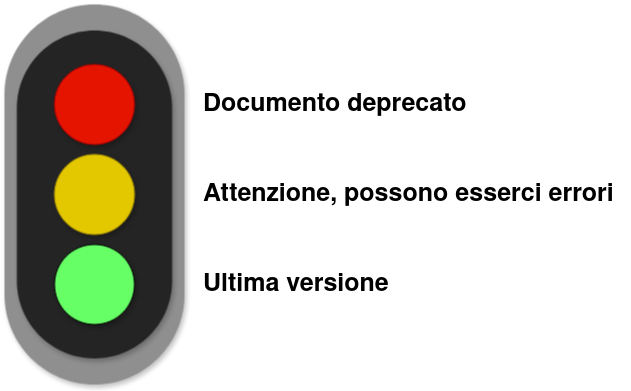
\includegraphics[scale=.35]{sources/Semaforo.drawio}
	\end{center}
\end{minipage}


\section{Repository del progetto}
Tutte le versioni del documento, insieme al codice sorgente e ai materiali aggiuntivi, sono disponibili nella \href{https://github.com/Giordi9902/unina_asd_notes}{repository} ufficiale su GitHub.

Ti invitiamo a consultare la repository per eventuali aggiornamenti, contributi o per segnalare problemi direttamente tramite issue.

\subsection{In caso di errori}
È sempre ben gradito ricevere feedback.

\textbf{Feedback generali:} se hai domande rispetto qualsiasi aspetto del libro non esitare a contattarmi:
\begin{itemize}
	\item Email: \texttt{giorgio99difusco@gmail.com}
\end{itemize}


\tableofcontents

\lstlistoflistings

% Chapter 1: Primo sguardo all'analisi algoritmica
\chapter{Primo sguardo all'analisi algoritmica}

\section{Definizione e proprietà degli algoritmi}

Prima d'iniziare ad analizzare un algoritmo dobbiamo prima capire cos'è un algoritmo.

\dfn{Algoritmo}{
    Un \textbf{algoritmo} è una procedura ben definita che prende un certo valore, o un insieme di valori, come \textbf{input} e genera un valore, o un insieme di valori, come \textbf{output}.
}

Quindi un algoritmo lo possiamo interpretare come \textit{una sequenza finita di passi} che,
se eseguiti da un \textbf{esecutore}, portano alla soluzione di un \textbf{problema computazionale} ben definito.

In generale un algoritmo gode delle seguenti proprietà:
\begin{itemize}
   \item \textbf{Non ambiguità:} tutti i passi che definiscono l'algoritmo devono essere non ambigui e chiaramente comprensibili dall'esecutore;
	\item \textbf{Generalità:} la sequenza di passi da eseguire dipende esclusivamente dal problema generale da risolvere, non dai dati che ne definiscono un'istanza specifica;
	\item \textbf{Correttezza:} un algoritmo è \textbf{corretto} se produce il risultato corretto a fronte di qualsiasi istanza del problema ricevuta in ingresso. Può essere stabilita, ad esempio, tramite:
	\begin{itemize}
		\item dimostrazione formale (matematica);
		\item ispezione informale;
	\end{itemize}
	\item \textbf{Efficienza:} misura delle risorse computazionali che esso impiega per risolvere un problema. Alcuni esempi sono:
	\begin{itemize}
		\item tempo di esecuzione;
		\item memoria impiegata;
		\item altre risorse: banda di comunicazione.
	\end{itemize}
\end{itemize}

\subsection{Il tempo di esecuzione di un algoritmo}

Spesso, quando si analizzano le proprietà di un algoritmo si parla di \textbf{complessità computazionale}. Questa può essere definita come segue:

\dfn{Complessità computazionale}{
    La \textbf{complessità computazionale} è il costo, in termini di tempo e memoria, necessari per eseguire un algoritmo, quindi per risolvere un problema.
}

Per determinare la complessità computazionale di un algoritmo bisognerà quindi definire al meglio il concetto di \textit{tempo di esecuzione}.

\dfn{Tempo di esecuzione}{
Il \textbf{tempo di esecuzione} di un programma per un particolare input è il numero di operazioni primitive che vengono eseguite o ``passi''.
}

Il tempo di esecuzione può dipendere da vari fattori:
\begin{itemize}
	\item Hardware su cui viene eseguito;
	\item Compilatore/Interprete utilizzato;
	\item Tipo e dimensione dell'input;
	\item Altri fattori: casualità
\end{itemize}

Una misura del costo computazionale soddisfacente deve:
\begin{enumerate}
    \item Basarsi su un \textbf{modello computazionale} in modo tale da poter definire il concetto di \textbf{passo algoritmico} nel modo più indipendente possibile dal tipo di esecutore;
    \item Svincolarsi dalla configurazione dei dati in ingresso, ad esempio basandosi sulle configurazioni più sfavorevoli (caso peggiore), così da garantire che le prestazioni nei casi reali saranno al più costose quanto il caso analizzato;
    \item Essere una funzione della dimensione dell'input;
    \item Essere asintotica, cioè fornire un'idea dell'andamento del costo all'aumentare della dimensione dell'input\footnote{Senza essere troppo precisi nell'analisi della grandezza di tale input. Nel nostro caso di studio infatti non stiamo considerando la macchina effettiva che esegue il calcolo.}.
\end{enumerate}

Una misura del costo computazione di un algoritmo deve quindi fornire una descrizione del costo asintotico nel caso peggiore, ovvero l'insieme degli input per i quali l'algoritmo richiede il massimo tempo di esecuzione.


\subsubsection{La macchina di Turing}\label{sez:Turing}
Alla base di un modello computazionale sta l'idea che ogni istruzione atomica abbia un \textbf{costo unitario}. Un noto modello computazionale è il modello della \textbf{macchina di Turing (MdT)}. Si tratta di una macchina astratta che manipola i dati contenuti su un nastro di lunghezza potenzialmente infinita, secondo un insieme prefissato di regole ben definite. Questo modello è largamente utilizzato nella teoria della calcolabilità e nello studio della complessità degli algoritmi, in quanto è di notevole aiuto agli studiosi nel comprendere i limiti del calcolo meccanico; la sua importanza è tale che oggi, per definire in modo formalmente preciso la nozione di algoritmo, si tende a ricondurlo alle elaborazioni effettuabili con macchine di Turing.

Una MdT, come mostrato in Figura \ref{fig:mdt}, è composta da:
\begin{itemize}
    \item Un \textbf{nastro di lunghezza infinita} costituito da celle le quali possono contenere una quantità d'informazione finita.
    \item Una \textbf{testina}, un \textbf{processore}, un \textbf{programma}
\end{itemize}

Le operazioni che può compiere in una \textbf{singola unità di tempo} sono:
\begin{itemize}
    \item Leggere o scrivere nella cella puntata attualmente dalla testina;
    \item Muoversi di una cella a destra, a sinistra oppure restare ferma.
\end{itemize}

\begin{center}
    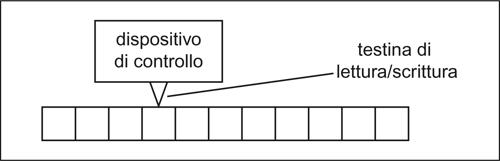
\includegraphics[scale = 0.4, origin = c]{res/Macchina_di_Turing.jpg}
    \captionof{figure}{Macchina di Turing}\label{fig:mdt}
\end{center}

\section{Algoritmo conta coppie}
Proviamo a studiare un algoritmo che fa quanto segue:
\begin{itemize}
    \item \textbf{Input:}  $n\in\mathbb{N}^*$, dove per $\mathbb{N}^*$ si intende $\mathbb{N}\setminus\{0\}$.
    \item \textbf{Output:} numero di coppie $(i,j)$ con $1\leq i\leq j\leq n$
\end{itemize}
Ad esempio, per $n=4$ abbiamo $10$ casi: $(1,1),(1,2),(1,3),(1,4),(2,2),(2,3),(2,4),(3,3),(4,4)$.

\subsection{Un metodo di risoluzione na\"if}
Il primo step per risolvere un problema difficile è quello di \textbf{decomporlo in problemi più semplici} seguendo l'approccio \emph{divide et impera}. L'idea quindi sarebbe quella di generare tutte le coppie e successivamente contare quelle che soddisfano la condizione posta. Si ottiene così:


\begin{lstlisting}[label=lst:Conta1, language=asd, caption={Conta1(n)}]
RIS = 0
for i = 1 to n do
    for j = 1 to n do
        if i <= j then
            RIS = RIS + 1
return RIS
\end{lstlisting}

Bisogna adesso porsi il problema di come associare un tempo di esecuzione all'Algoritmo \ref{lst:Conta1}. Nel farlo assumiamo che il valore dell'input sia \textbf{misura della complessità dell'algoritmo}\footnote{In generale non sarà così ma assumiamo che nel nostro modello computazionale i dati vengano rappresentati attraverso un sistema unario.}. Analizziamo la complessità di \textit{ogni linea} contandone le operazioni elementari e valutando il numero di volte in cui queste vengono eseguite:
\begin{enumerate}
  \item L'istruzione contiene una singola operazione elementare che viene eseguita a tempo costante.
  \item Il ciclo \texttt{for} viene eseguito $n+1$ volte. Infatti, oltre alle $n$ iterazioni date dall'estremo superiore, viene effettuata un'iterata in più per il controllo che permette all'esecutore di uscire dal ciclo una volta che la condizione risulta falsa. Il contributo della riga sarà quindi:
	\begin{displaymath}
		2 \cdot \sum_{i=1}^{n+1}=2 \cdot (n+1)
	\end{displaymath}
  \item Questo ciclo si trova annidato al primo ciclo \texttt{for}. Quindi ciascuna delle sue $n+1$ iterazioni sarà ripetuta $n$ volte. In totale:
	\begin{displaymath}
		2 \cdot \sum_{i=1}^{n} (\sum_{j=1}^{n+1} 1 )= 2 \cdot \sum_{i=1}^{n}(n+1)=2 \cdot n \cdot (n+1)
	\end{displaymath}
  \item L'istruzione \texttt{if} si trova all'interno dei due cicli for, sarà quindi ripetuta:
	\begin{displaymath}
		3 \cdot \sum_{i=1}^{n}(\sum_{j=1}^{n} 1) = 3 \cdot n^{2}
	\end{displaymath}
	volte.
  \item È impossibile determinare a priori il numero di volte in cui l'istruzione all'interno dell'istruzione \texttt{if}, essendo questo dipendente dal soddisfacimento o meno della condizione imposta alla coppia $(i,j)$. Nel caso in questione possiamo osservare che, se $i=1$, il corpo dell'\texttt{if} viene eseguito $n$ volte; con $i=2$ viene eseguito $n-1$ volte, $\ldots$ con $i=k$ viene eseguito $n-(k-1)$, dove $k$ è il valore corrente di $i$. In generale:
  \begin{displaymath}
  \sum_{i=1}^{n} (n-i+1)
  \end{displaymath}
\end{enumerate}

Per calcolare l'ultima sommatoria basta spezzarla in tre sommatorie:
\begin{equation}
    \sum_{i=1}^{n} (n-i+1) = \sum_{i=1}^{n} n - \sum_{i=1}^{n} i + \sum_{i=1}^{n} 1 = n^2 - \frac{n(n+1)}{2} + n = n(n+1) - \frac{n(n+1)}{2} = \frac{n(n+1)}{2}
\end{equation}

Ora per calcolare il tempo di esecuzione, basta sommare:
\begin{eqnarray*}
    T_1(n) &=& 1+ 2\cdot(n+1) + 2\cdot(n^{2}+n)+3n^{2} + \frac{n(n+1)}{2} \\
    &=& 1 + 2n + 2 + 2n^2 + 2n + 3n^2 + \frac{n^2}{2} + \frac{n}{2} \\
    &=& \frac{11}{2}n^2 + \frac{9}{2}n + 4
\end{eqnarray*}

Il nostro algoritmo ha tempo \textbf{quadratico}. È facile convincersi del fatto che l'algoritmo\ref{lst:Conta1} è molto laborioso in quanto deve generare ben $n^{2}$ coppie quando potrebbe sicuramente generarne di meno.

\subsection{Migliorare l'algoritmo tramite l'analisi}
L'analisi del tempo di esecuzione dell'Algoritmo \ref{lst:Conta1} ci ha permesso di prevedere all'$i$-esima iterazione del \texttt{for} a linea 2 quante volte veniva eseguita il corpo dell'\texttt{if}. Proviamo a usare questa conoscenza a nostro vantaggio per migliorare l'algoritmo.

Ciò che si era notato era che, fissato $i$, non c'è bisogno di effettuare alcun controllo in quanto il numero di coppie $(i,j)$ che soddisfano alla nostra condizione è pari a $\displaystyle\sum_{i=1}^{n} (n-i+1)$, ovvero:
\begin{equation}
    \frac{n(n+1)}{2}
\end{equation}

A questo punto proviamo a scrivere il nuovo codice utilizzando questo concetto.

\begin{lstlisting}[label = lst:Conta2, language=asd, caption={Conta2(n)}]
RIS = 0
for i = 1 to n do
    RIS = RIS + (n-i+1)
return RIS
\end{lstlisting}

Analizzando nuovamente, istruzione per istruzione, il costo computazionale dell'algoritmo si evince che $T_2(n) = 9n+4$. Infatti:
\begin{enumerate}
  \item Tempo costante;
  \item $2\ \displaystyle\sum_{i = 1}^{n+1} 1 = 2n+2$;
  \item $(3+3+1) n = 7n$;
  \item Tempo costante.
\end{enumerate}

Il nostro algoritmo è migliorato in quanto adesso il tempo di esecuzione è lineare. Da quadratico a lineare è un grande miglioramento, ma possiamo fare di meglio. Infatti, adesso l'algoritmo non fa nient'altro che calcolare $\displaystyle\sum_{i=1}^{n} i$ di cui, come abbiamo già osservato, esiste una diretta correlazione con la somma dei primi $n$ numeri. I due problemi sono infatti isomorfi. Dunque abbiamo:

\begin{lstlisting}[label = lst:Conta3, language=asd, caption={Conta3(n)}]
RIS = (n(n+1))/2
return RIS
\end{lstlisting}

\textbf{Tempo di esecuzione per ogni istruzione:}
\begin{enumerate}
  \item 2 + 3 = 5
  \item 1
\end{enumerate}

Dall'analisi si evince che $T_3(n) = costante$.


\section{Somma della massima sottosequenza}\label{sottosequenzecontigue}
Proviamo a studiare un algoritmo che fa quanto segue:
\begin{itemize}
    \item \textbf{Input:}  $n\in\mathbb{N}^*, A$. Dova A è un array di dimensione N
    \item \textbf{Output:} La somma della massima sotto-sequenza di A
\end{itemize}

\begin{example}
		Sia $n=7$, e consideriamo l'array: \{1, -3, 8, 2, -10, 1, 7\}. In questo caso, la massima sottosequenza ha somma 10, infatti: $MaxSum = 8+2$.
\end{example}

\subsection{Introduzione e prima risoluzione del problema}
Una prima idea, potrebbe essere quella di applicare un algoritmo \textit{\textbf{brute force}}.
Quindi dobbiamo applicare i seguenti passi:
\begin{enumerate}
    \item Generare tutte le possibili sotto-sequenze.
    \item Calcolarne la somma.
    \item Aggiornare il max.
\end{enumerate}

Per generare tutte le possibili sotto-sequenze possiamo scegliere di rappresentarla con una coppia $(i, j)$, dove $i$ è l'indice del primo elemento, e $j$ quello dell'ultimo, tale che $i\leq j$.


\begin{lstlisting}[label = MaxSum1, language=asd, caption={MaxSum1(A,n)}]
MAX = 0
    for i=1 to n do
        for j=i to n do
            SUM = 0
            for k=i to j do
                SUM = SUM + A[k]
            if SUM > MAX then
                MAX = SUM
return MAX
\end{lstlisting}

Effettuando un'analisi non approfondita ci rendiamo conto dai tre cicli \texttt{for} innestati che l'algoritmo in questione ha un costo cubico $(T_1 = O(n^3))$ rispetto all'input. Notare che nell'algoritmo \ref{MaxSum1} vengono effettuate diverse volte le stesse operazioni, questo perché andiamo a calcolare ogni volta da capo la somma, infatti:
\begin{equation}
    \sum_{k=i}^{j+1} A[k] = \sum_{k=i}^{j} A[k] + A[k+1]
\end{equation}

Dove $\displaystyle\sum_{k=i}^{j} A[k]$ è l'operazione ripetuta più volte. Per migliorare questo aspetto, possiamo conservare la somma e aggiungere solo il successivo per ogni sequenza. Vediamo come evolve il codice dopo questa modifica.

\begin{lstlisting}[label = MaxSum2, language=asd, caption={MaxSum2(A,n)}]
MAX = 0
for i=1 to n do
    SUM = 0
    for j=i to n do
        SUM = SUM + A[j]
        if SUM > MAX then
            MAX = SUM
return MAX
\end{lstlisting}

Questa modifica ci consente di ridurre il costo del nostro algoritmo da cubico a quadratico. $T_2 = (O(n^2))$.

\subsection{Algoritmo \textsc{MaxSum} lineare}

Prima di procedere a scrivere l'algoritmo, fermiamoci a ragionare sul come possiamo ``scartare'' parti di array, in modo da non doverlo controllare tutto per cercare la massima sotto-sequenza. Per semplicità consideriamo di avere solo tre valori: $a$, $b$, $c$. Di questi, ipotizziamo siano vere:
\begin{enumerate}
    \item $a<b$;
    \item $b<c$.
\end{enumerate}
Quindi per transitività sappiamo che $a<c$. Potrà sembrare una banalità, ma così facendo risparmiamo un confronto, ed è proprio la chiave per ottimizzare l'algoritmo. Ipotizziamo sia vero quanto segue:

\begin{equation}
    \sum_{z=i}^{j} A[z] \geq 0 \text{ , con } i \leq j \leq r-1
\end{equation}

Si hanno allora due possibili casi:

\begin{enumerate}
    \item $\displaystyle\sum_{z=i}^{r} A[z] \geq 0$, allora:
    \begin{displaymath}
        \sum_{z=i}^{k} A[z] = \sum_{z=i}^{j} A[z] + \displaystyle\sum_{z=j+1}^{k} A[z] \geq \displaystyle\sum_{z=j+1}^{k} A[z]
    \end{displaymath}
    Se $a$ un numero sommo una quantità positiva, ottengo un numero più grande, banalmente. Di conseguenza
    è inutile calcolare le sottosequenze interne ad $i$ ed $r$.

    \item $\displaystyle \sum_{z=i}^{r} A[z] < 0$, allora:

    \begin{displaymath}
        \sum_{z=j}^{k} A[z] = \sum_{z=i}^{r} A[z] + \sum_{z=r+1}^{k} A[z] < \sum_{z=r+1}^{k} A[z]
    \end{displaymath}

    Sappiamo che la prima sommatoria è negativa semplicemente perché per ipotesi $\displaystyle\sum_{z=i}^{j-1} A[z] + \sum_{z=j}^{r} A[z] < 0$.

    Ricapitolando, $\displaystyle\sum_{z=j}^{k} A[z] \leq \sum_{z=r+1}^{k} A[z]$, cioè è inutile calcolare ogni sottosequenza che inizia tra $i$ ed $r$ e termina oltre $r$.
\end{enumerate}

Facendo questa analisi siamo riusciti a eliminare un gran numero di calcoli e confronti superflui. Andiamo a vedere come evolve l'algoritmo.


\begin{lstlisting}[label = lst:MaxSum3, language=asd, caption={MaxSum3(A, n)}]
MAX = 0
SUM = 0
for i=1 to n do
    SUM = SUM + A[i]
    if SUM < 0 then
        SUM = 0
    else
        MAX = MAX(SUM, MAX)
return MAX
\end{lstlisting}

Andando a fare un'analisi del codice vediamo che abbiamo un solo \texttt{for} che va da $1$ a $n$, ovvero, andiamo a eseguire tante istruzioni quanto $n$.

In conclusione, andando a eliminare confronti e calcoli superflui, siamo riusciti nell'intento di rendere il nostro algoritmo lineare. $T_3 = O(n)$.

% Chapter 2: Strutture dati elementari
\chapter{Strutture dati elementari}

\section{Che cos'è una struttura dati}
Gli insiemi rappresentano un concetto fondamentale per l'informatica e la matematica. Mentre gli insiemi matematici sono immutabili, gli insiemi manipolati dagli algoritmi possono crescere, ridursi o cambiare nel tempo. Per questo motivo questi insiemi sono detti \textit{\textbf{dinamici}}.

\dfn{Insieme Dinamico}{
    Sia n $\geq$ 0 e sia S = $\{e_1, e_2,..., e_n\}$  un \textit{\textbf{insieme}}, cioè una collezione di oggetti distinguibili, che si denotano come elementi (o attributi). Un insieme è detto \textit{\textbf{dinamico}} se e soltanto se la sua cardinalità può variare nel tempo, cioè può variare il numero dei suoi elementi.
}
 Gli algoritmi per la risoluzione di un problema possono richiedere vari tipi di operazioni da svolgere sugli insiemi.

\dfn{Struttura dati astratta}{
    Si dice \textbf{struttura dati astratta} un insieme dinamico definita da un punto di vista logico, descrivendo cioè soltanto le associazioni logiche tra i dati e le operazioni mediante le quali utilizzare la struttura.
}

Le \textbf{caratteristiche} principali che differenziano le strutture dati astratte sono:
\begin{itemize}
	\item La possibilità di cambiare o meno dimensione durante l'esecuzione (\textbf{dinamica} o \textbf{statica});
	\item Il fatto che i dati siano tutti dello stesso tipo oppure no (\textbf{omogenea} o \textbf{eterogenea});
	\item Il fatto che sia possibile accedere direttamente a un elemento, o che sia invece necessario scorrere tutti gli elementi precedenti (\textbf{accesso diretto} o \textbf{sequenziale});
\end{itemize}

\dfn{Struttura dati concreta}{
    Una struttura dati \textbf{concreta} è la rappresentazione nella memoria del computer di una struttura dati astratta.
}

\begin{example}
Un esempio di struttura dati astratta potrebbe essere una sequenza di numeri, una sua possibile struttura concreta può essere un vettore.
\end{example}

La caratteristica principale che differenzia le strutture di dati concrete è il fatto che i dati siano memorizzati in memoria in locazioni di memoria contigue oppure no. Le strutture dati vengono memorizzate in memoria ed esistono soltanto all'interno del programma che le utilizza; quando il programma termina, i dati inseriti nella struttura non sono più utilizzabili; non è possibile conservare dati in queste strutture, né usarle per comunicare dati tra un programma e un altro.

\subsection{Gli elementi di un insieme dinamico}
In una tipica implementazione di un insieme dinamico, ogni elemento è rappresentato da un oggetto i cui attributi possono essere esaminati e manipolati se c'è un puntatore all'oggetto. Per alcuni tipi di insiemi dinamici si suppone inoltre che uno degli attributi dell'oggetto sia una \textbf{chiave} di identificazione. Se le chiavi sono tutte diverse, possiamo pensare all'insieme dinamico come a un insieme di valori chiave. L'oggetto può contenere \textbf{dati satelliti}, che vengono trasportati in altri attributi dell'oggetto oppure includere ulteriori attributi che possono essere manipolati dalle operazioni svolte sull'insieme; questi attributi possono contenere dati o puntatori ad altri oggetti dell'insieme.

\subsection{Operazioni sulle strutture dati}
Le operazioni su un insieme dinamico possono essere raggruppate in due categorie: le \textbf{interrogazioni} che restituiscono semplicemente informazioni sull'insieme; le \textbf{operazioni di modifica} che cambiano l'insieme.

Consideriamo un insieme con una relazione d'ordine $\leq$ e assumiamo che l'elemento \textsc{NIL} non sia mai presente all'insieme $(S, \leq)$. Per tale insieme possiamo definire le seguenti operazioni:

\begin{itemize}
	\item \textsc{Ricerca}(S,k): restituisce un elemento di S oppure \textsc{nil} se $k \notin S$.
	\item \textsc{Inserimento}(S,k): restituisce un nuovo insieme $S' = S \cup \{k\}$.
	\item \textsc{Cancellazione}(S,k): restituisce un nuovo insieme $S' = S \setminus \{k\}$.
\end{itemize}

Gli algoritmi per le operazioni sugli insiemi sfruttano le caratteristiche della rappresentazione dell’insieme e questo significa che le operazioni di modifica (inserimento e cancellazione) \textbf{dovranno mantenere intatte quelle caratteristiche} (ad esempio se devo aggiungere un elemento in una sequenza ordinata, devo aggiungerlo nella giusta posizione in modo da lasciare ordinata la sequenza). Chiaramente la ricerca è un operazione che non modifica la struttura dati e quindi preserva naturalmente le proprietà della struttura, mentre per le altre due, più vincoli avremo e più complesso sarà definire delle operazioni.

L'operazione di ricerca non si limita solo alla ricerca dell'elemento $k$ nell'insieme $S$, posso infatti ampliare tale operazione con altre operazioni di ricerca:
\begin{itemize}
	\item \textsc{Successore}(S,k): restituisce l'elemento con la più piccola chiave $a > k$.
	\item \textsc{Predecessore}(S,k): restituisce l'elemento con la più grande chiave $a < k$.
	\item \textsc{Minimo}(S,k): restituisce un puntatore all'elemento di S con la chiave più piccola.
	\item \textsc{Massimo}(S,k): restituisce un puntatore all'elemento di S con la chiave più grande.
\end{itemize}

\section{Array}
L'\textbf{array} è un potente strumento ampiamente usato in programmazione. Gli array servono ad immagazzinare ed organizzare i dati nella memoria di un calcolatore: la loro potenza deriva soprattutto dal fatto che forniscono un modo molto semplice ed efficace di eseguire e fare riferimento a computazioni su collezioni di dati che condividono attributi comuni.

\dfn{Array}{
    Un \textit{\textbf{array}} è un insieme \textit{\textbf{statico}}, in cui la \textit{dimensione} dello stesso è dunque \textit{prefissata}.
}

È possibile vedere gli array come un'applicazione fatta in questo modo:
\begin{equation}
\forall n \in \mathbb{N}, I_{n} = \{0,1,2,...,n-1\} \mapsto d \in A
\end{equation}
La quale ha come dominio l'insieme dei primi $n$ numeri e come codominio gli elementi contenuti nell'array. Per denotare quindi l'$i$-esimo elemento di $A$ si è soliti utilizzare la seguente notazione: $A[i] = d$.
Un modo alternativo per vedere l'array è considerarlo come l'unione di ciascuno dei suoi singoli elementi, ovvero:
\begin{equation}
A = \bigcup_{i=0}^{n-1} \{A[i]\}
\end{equation}

\subsection{Il problema dell'inserimento}
Affrontiamo ora il problema dell'inserimento in un array. Consideriamo quindi la nostra struttura dati fatta in questo modo:
\begin{center}
    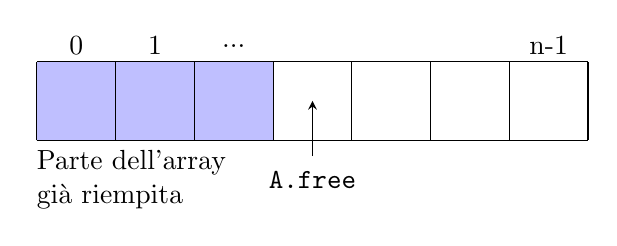
\begin{tikzpicture}
        \fill[blue, nearly transparent] (0,0) rectangle (3,-1);
        \draw (0,0) grid (7,-1);
        \node at (0.5,0.2) {0};
        \node at (1.5,0.2) {1};
        \node at (2.5,0.2) {...};
        \node at (6.5,0.2) {n-1};
        \node at (3.5,-1.5) {\texttt{A.free}};
        \draw [-stealth](3.5,-1.2) -- (3.5,-0.5);
        \node[align=left] at (1.2,-1.5) {Parte dell'array\\già riempita};
    \end{tikzpicture}
\end{center}

In questa struttura abbiamo un puntatore chiamato \texttt{A.free} che mira alla prima cella vuota dell'array. Se volessimo inserire un nuovo elemento, ammesso che l'array non sia pieno, si tratterebbe semplicemente di eseguire una operazione a \textit{tempo costante}. Questo perché l'array è una struttura che gode di \textbf{accesso diretto} alla memoria, grazie al fatto che le celle dell'array sono \textit{contigue}. Per i vari casi di studio che seguiranno, si faranno le seguenti assunzioni:

\begin{itemize}
    \item S è un insieme di dati dinamico contenuto in un intervallo contiguo di A (la cui lunghezza è predeterminata);
    \item S non ammette duplicati;
\end{itemize}

Per inserire un nuovo elemento all'interno del vettore, la prima operazione da effettuare è quella di assicurarsi che l'elemento non sia già presente nella struttura dati. Essendo l'array non ordinato, il problema della ricerca si riduce nell'esecuzione lineare di una lettura ed un confronto, a partire dall'inizio o dalla fine della struttura, fino all'esaurimento dell'array. Tale operazione ci tornerà parecchio utile sia per l'inserimento che per la cancellazione di un elemento in un vettore.

\begin{lstlisting}[label = lst:SearchInArray, language=asd, caption={Search(A,k)}]
pos = A.free - 1
while (A[pos] != k && pos >= 0) do
	pos = pos - 1
return pos
\end{lstlisting}

L'algoritmo \ref{lst:SearchInArray} restituisce la posizione dell'elemento nell'array se l'ha trovato, altrimenti restituisce -1. Andando a fare un'analisi approssimativa del codice è facilmente osservabile che l'algoritmo ha un \textit{tempo di esecuzione lineare} dato dal controllo sequenziale di ogni singola cella del vettore. Di conseguenza il caso peggiore, nel caso della ricerca di un elemento in un vettore non ordinato, è ottenuto nel caso in cui l'array sia pieno, ovvero quando \texttt{A.free = n-1}.

Grazie all'algoritmo di ricerca è possibile implementare gli algoritmi di inserimento e rimozione di un elemento. Infatti, prima di eseguire tali operazioni bisogna innanzitutto verificare la presenza dell'elemento nell'insieme. Nel caso dell'inserimento di un nuovo elemento, qualora il vettore dovesse essere già pieno, è possibile adoperare una funzione usiliaria \texttt{Resize} che effettui il ridimensionamento del vettore\footnote{Allocando una porzione di memoria maggiore ed eseguendo la copia degli elementi dell'array originale  nel nuovo vettore così ottenuto.}. Nel caso della cancellazione di un elemento, invece, non è necessario effettuare alcun ridimensionamento ma semplicemente sostituire all'interno della cella in cui si trova l'elemento da cancellare con il valore dell'ultimo elemento dell'array ed infine decrementare \texttt{A.free} di 1.

\begin{center}
	\begin{minipage}{0.4\textwidth}
	\begin{lstlisting}[label = lst:InsertInArray, language=asd, caption={Insert(A,k)}]
pos = Search(A, k)
if (pos == -1) then
	if (A.free == length(A)) then
		A = Resize(A)
	A[A.free] = k
	A.free = A.free + 1
\end{lstlisting}
\end{minipage}
\begin{minipage}{0.4\textwidth}
	\begin{lstlisting}[label = lst:DeleteInArray, language=asd, caption={Delete(A,k)}]
pos = Search(A, k)
if (pos >= 0) then
    A[pos] = A[A.free-1]
    A.free = A.free - 1
\end{lstlisting}
\end{minipage}

\end{center}

Consideriamo il caso in cui l'insieme dinamico memorizzato nell'array sia un insieme all'interno del quale è stata definita una relazione d'ordine $\leq$. In questa situazione ogni elemento dell'array deve soddisfare alla seguente condizione:
\begin{displaymath}
	\forall i \bigl(\ 1 \leq i \leq n \Rightarrow S[i]\leq S[i+1]\bigr)
\end{displaymath}
Grazie a questo vincolo aggiuntivo possiamo osservare che è possibile migliorare notevolmente le operazioni di ricerca. Infatti, nel caso dei vettori non ordinati, la ricerca dell'elemento massimo o minimo richiede sempre tempo lineare dovendo scorrere l'array nella sua interezza mentre, in un vettore ordinato, l'operazione richiede una singola operazione di lettura del primo elemento (nel caso della ricerca del minimo) o dell'ultimo elemento del vettore (nel caso della ricerca del massimo).

Nonostante i vantaggi ottenuti, nel caso della ricerca di un elemento, notiamo un peggioramento dal punto di vista computazionale nel caso delle operazioni di inserimento e cancellazione. Infatti, se volessimo inserire un nuovo elemento nell'array si può constatare facilmente che questo genere di operazione sia più complicata nel caso degli array ordinati in quanto prima di inserire un qualsiasi elemento sarà necessario cercare il suo precedente, far slittare gli elementi successivi e infine mettere l'elemento nella casella appena liberata.

Per un array non ordinato, al contrario, l'operazione si esegue facilmente a tempo costante in quanto basterebbe inserire il nuovo elemento alla fine del vettore. Scegliere i \textbf{vincoli della struttura dati} ha un impatto rilevante sulla complessità delle operazioni. Il punto di equilibrio dipenderà da fattori quali la dinamicità dell'insieme sul quale si sta operando, il numero di operazioni che si vogliono eseguire e la frequenza delle stesse. Da questo breve esempio si deduce che non esiste una struttura dati ``perfetta'': tutto dipende dalle operazioni che si vogliono eseguire su di esse.

\subsection{La ricerca binaria}
Come già detto in precedenza, mentre negli array non ordinati il problema della ricerca richiede sempre un tempo lineare, negli array ordinati il problema può essere risolto in \textit{tempo logaritmico}. Sfruttando infatti la proprietà dell'ordinamento è possibile definire un algoritmo ricorsivo chiamato \textsc{Ricerca-Binaria} oppure \textsc{Ricerca-Dicotomica} il quale confronta la chiave $key$ ricercata con quella dell'elemento centrale dell'array: se questa è uguale, la ricerca termina con successo, se è maggiore, la ricerca procede richiamando lo stesso metodo sulla prima metà dell'array mentre, se è minore, nella seconda metà dell'array. In sintesi \textsc{Ricerca-Binaria} opera nel seguente modo:
\begin{enumerate}
	\item Divide la sequenza che prende in ingresso determinando il valore $q= \lfloor n/2 \rfloor$;
	\item Effettua il controllo $S[q]=key$, dove $key$ è il valore da ricercare; se la condizione è falsa allora:
	\begin{enumerate}
		\item Se $S[q]<key$ allora richiama se stesso nella sottosequenza di destra;
		\item Se $S[q]>key$ allora richiama se stesso nella sottosequenza di sinistra.
	\end{enumerate}
\end{enumerate}

\begin{lstlisting}[label = lst:BinSearchRec, language=asd, caption={BinSearchRec(A,k,i,j)}]
if (i <= j) then
    q = @$\lfloor$@(i+j)/2@$\rfloor$@
    if (A[q] < k) then
        ret = BinSearchRec(A, k, q+1, j)
    else if (A[q] > k) then
        ret = BinSearchRec(A, k, i, q-1)
    else
        ret = q
else
    ret = -1
return ret
\end{lstlisting}

Ora andiamo a fare un'analisi di questo algoritmo per vedere se abbiamo effettivamente migliorato il tempo di esecuzione. Localmente ogni chiamata della funzione ha tempo costante $c$, quindi per calcolare il tempo di esecuzione dell'algoritmo basta fare \[T_{Bs}(n) = \sum_{l=0}^{h+1} c\] dove $l$ rappresenta il livello della chiamata che stiamo eseguendo ed $h+1$ è il livello che corrisponde o al caso $A[q] = k$ oppure al caso $i<j$ dove l'elemento non è presente. A questo punto bisogna capire chi è $h$. Per fare ciò ci basta osservare che ad ogni chiamata ricorsiva andiamo sempre a considerare la metà dell'array mentre nell'ultima chiamata si considera una sola cella. Quindi:

\begin{equation}
\frac{n}{2^h} = 1 \iff n = 2^h \iff \log_2(n) = \log_2(2^h) \iff \log_2(n) = h
\end{equation}

Sostituendo nella sommatoria, otteniamo:

\begin{equation}\label{eq:ricbin1}
    \sum_{l=0}^{h+1} c = \sum_{l=0}^{\log_2(n)+1} c = c \sum_{l=0}^{\log_2(n)+1} 1 = c\log_2(n) + c
\end{equation}

Dall'equazione \ref{eq:ricbin1} osserviamo che il tempo di esecuzione della ricerca binaria $T_{Bs}(n)$ è logaritmica rispetto alla dimensione dell'array il che rappresenta un notevole miglioramento rispetto all'algoritmo \textsc{Search(A,k)} il quale abbiamo visto avere un costo computazionale lineare rispetto alla grandezza del vettore. Tuttavia, nonostante il risparmio di tempo dato dalla ricerca binaria, non si può dire altrettanto per gli altri algoritmi di inserimento e cancellazione (\textsc{Insert} e \textsc{Delete}) i quali richiedono un tempo lineare rispetto alla dimensione del vettore. Infatti, inserire un singolo elemento all'interno di un vettore non ordinato prevede innanzitutto la ricerca della posizione corretta dove inserire l'elemento che ha un costo logaritmico, lo slittamento di una posizione degli elementi del vettore il quale può avere alla peggio un costo lineare se l'elemento viene inserito nella prima cella più il costo dato dall'assegnazione che viene eseguito a tempo costante:
\[T_{insert} = \log_{2}(n)+n+C\]

Invece, nel caso di un inserimento che necessita anche il ridimensionamento del vettore mediante la funzione \textsc{Resize} si ha un overhead lineare aggiuntivo dato dalla copia di tutti gli elementi.

Al fine di ridurre il tempo di esecuzione dato dall'operazione di ridimensionamento, si può pensare di allocare nuova memoria per una grandezza doppia rispetto alla lunghezza del vettore originale, anziché limitarsi ad aggiungere una sola cella. In questo modo infatti si riduce in maniera logaritmica la necessità di dover ridimensionare il vettore a fronte di un nuovo inserimento.

\section{Liste concatenate}

\dfn{Lista concatenata}{
    Una \textit{\textbf{lista concatenata}} è un insieme dinamico in cui ogni elemento ha una chiave (\textit{key}) ed un riferimento all'elemento successivo
    (\textit{next}) dell'insieme. È una struttura ad accesso \textit{\textbf{sequenziale}}. Il singolo elemento di una lista è chiamato \textit{\textbf{nodo}}.
}

Per capire meglio come poter definire una lista, proviamo a considerare la sommatoria dei primi $n$ numeri:

\begin{displaymath}
    \sum_{i=0}^{n} i = \left \lbrace \begin{array}{ll}
                            0 & \mbox{se } n = 0 \\
                            n + \displaystyle\sum_{i=0}^{n-1} & \mbox{se }n \geq 1
                        \end{array} \right.
\end{displaymath}

Con questa definizione possiamo calcolare la sommatoria dei primi $n$ numeri, la quale è pari a 0 se $n=0$ ed è pari a $n$ più la sommatoria dei primi $n-1$ numeri quando $n\geq 1$. Allo stesso modo, possiamo definire una lista $L$ nel seguente modo:
	\begin{equation}\label{definizione:listaconcatenata}
		L=\left\lbrace
		\begin{array}{lc}
			\varnothing & \mbox{se vuota}\\
			\mbox{Un nodo con un puntatore ad una lista L'} & \mbox{altrimenti}
		\end{array}
		\right.
	\end{equation}

Una lista può avere varie forme: può essere singolarmente o doppiamente concatenata, ordinata oppure no, circolare oppure no. In una lista \textbf{semplicemente concatenata} è presente, oltre all'attributo chiave, un secondo attributo chiamato \textit{\textbf{next}} contenente l'indirizzo di memoria del nodo successivo. Nelle \textbf{liste doppiamente concatenate} è presente anche l'attributo \textit{\textbf{prev}} contenente un puntatore al nodo precedente. Dato un nodo $x$, se $x.prev=NIL$, l'elemento $x$ non ha un predecessore e quindi è il primo elemento della lista, chiamato \textbf{testa} o \textbf{head} della lista. Se $x.next=NIL$, l'elemento $x$ non ha successore e quindi è l'ultimo elemento della lista, che è detto anche \textbf{coda} o \textbf{tail}. Un attributo $L.head$ punta al primo elemento della lista. Se $L.head=NIL$, la lista è vuota.

Se una lista è \textbf{ordinata} l'ordine lineare della lista corrisponde all'ordine lineare delle chiavi memorizzate negli elementi della lista; l'elemento minimo è la testa della lista e l'elemento massimo è la coda della lista. Una lista può essere \textbf{non ordinata}; gli elementi di questa lista possono presentarsi in qualsiasi ordine. In una \textbf{lista circolare}, il puntatore \textit{prev} della testa della lista punta alla coda e il puntatore \textit{next} della coda della lista punta alla testa.

Una struttura del genere ha i suoi vantaggi dal punto di vista computazionale, come l'inserimento e la cancellazione (se sono sull'elemento da cancellare) a tempo costante, ma anche i suoi svantaggi, ovvero proprio il fatto che si ha un accesso \textit{sequenziale} alla memoria. Ciò significa che, per raggiungere un elemento della lista, bisognerà necessariamente scorrere tutta la struttura fino al nodo richiesto.

\subsection{Ricerca in una lista concatenata}
Data la struttura particolare delle liste concatenate non è possibile accedere direttamente ad un qualsiasi elemento come accade negli array bensì è necessario scorrere ogni nodo a partire dalla testa fino a quando non si trova l'elemento desiderato. Questo significa che per accedere ad un nodo di una lista $L$ è necessario effettuare una semplice ricerca lineare che restituisce un puntatore al nodo ricercato. Anche supponendo di avere una lista ordinata doppiamente concatenata e voler implementare la ricerca binaria, per raggiungere l'elemento della sottosequenza di grandezza $n/2^{i}$ bisogna partire dall'indice mediano della sequenza precedente; quindi il costo complessivo sarà:
\begin{displaymath}
	\sum_{i=1}^{\log n} \bigl(\frac{n}{2^{i}}\bigl)=n\sum_{i=1}^{\log n} \bigl(\frac{1}{2}\bigl)^{i}=n-1
\end{displaymath}
\begin{center}
	\begin{minipage}{0.4\textwidth}
	\begin{lstlisting}[label = lst:SearchRec, language=asd, caption={SearchRec(L, k)}]
ris = NULL
if (L != NULL) then
    if (L->key = k) then
        ris = L
    else
        ris = Search(L->next, k)
return ris
\end{lstlisting}
\end{minipage}
\begin{minipage}{0.4\textwidth}
	\begin{lstlisting}[label = lst:SearchIter, language=asd, caption={SearchIter(L, k)}]
ris = NULL
tmp = L
while (tmp != NULL && ris = NULL) then
    if (L->key = k) then
        ris = tmp
    else
        tmp = tmp->next
return ris
\end{lstlisting}
\end{minipage}
\end{center}

\subsection{Inserimento in una lista non ordinata}

Dato un nodo $x$, l'algoritmo \textsc{List-Insert}(Algoritmo \ref{lst:InsertList}) inserisce un nodo con chiave \texttt{x} nella testa della lista concatenata sfruttando il fatto che ogni elemento della lista è indipendente dagli altri e non sono disposti in maniera contigua. Questa operazione prende il nome di \textbf{inserimento in testa}. Prima di eseguire l'inserimento bisogna invocare una funzione \textsc{NewNode} per la creazione di un nuovo nodo.
\begin{center}
\begin{minipage}{0.4\textwidth}
\begin{lstlisting}[label=lst:NewNode, language=asd, caption={NewNode(k)}]
tmp = AllocaNodo()
tmp->key = k
return tmp
\end{lstlisting}
\end{minipage}
\begin{minipage}{0.4\textwidth}
\begin{lstlisting}[label=lst:InsertList, language=asd, caption={Insert(L, k)}]
ret = Search(L, k)
if (ret == NULL) then
	tmp = NewNode(k)
	tmp->next = L
	L = tmp
return L
\end{lstlisting}
\end{minipage}
\end{center}
\subsection{Inserimento in una lista ordinata}
Inserire un nodo all'interno di una lista ordinata non ha lo stesso costo dell'inserimento in testa. Infatti prima di poter inserire il nodo bisogna garantire il vincolo dell'ordinamento andando a fare una ricerca della posizione esatta in cui andare ad inserire il nuovo nodo, più precisamente andando a cercare all'interno della lista il nodo \textbf{predecessore}. L'algoritmo che si ottiene avrà quindi un costo lineare dato dall'operazione di ricerca. Si ha così l'algoritmo \textsc{InsertInOrderedList(L,k)}.

\begin{lstlisting}[label=lst:InsertInOrderedList, language=asd, caption={InsertInOrderedList(L, k)}]
tmp = L
p = NULL
while (tmp != NIL && tmp->key < k) do	// Ricerca del predecessore
    p = tmp
    tmp = tmp->next
if (tmp == NIL || tmp->key > key) then // Inserimento di un nuovo nodo
    new = NewNode(tmp, k)
    if (p != NIL) then	// Se esiste il predecessore si aggiorna il successivo
        p->next = new
    else	// Altrimenti si inserisce in testa
        L = new
return L
\end{lstlisting}

\begin{lstlisting}[label = lst:InsertInOrderRec, language=asd, caption={InsertInOrder-Rec(L,k)}]
if (L == NIL || L->key > k) then
    L = NewNode(L, k)
else (if L->key < k) then
    L->next = InsertInOrderRec(L->next, k)
return L
\end{lstlisting}

\subsection{Cancellazione di un nodo in una lista}
La cancellazione di un nodo da una lista non può essere fatto con un costo minore del lineare, che sia ordinata o meno la lista. Infatti la cancellazione comprende due passi: la ricerca del nodo con la chiave $k$ e la cancellazione del nodo e l'aggiornamento dei puntatori del nodo precedente e di quello successivo. Si ottiene così l'algoritmo \textsc{Cancella}$(L,k)$. Si supponga che la lista non contenga duplicati.

\begin{center}
	\begin{minipage}{0.4\textwidth}
	\begin{lstlisting}[label=lst:DeleteIter,language=asd,caption={\textsc{DeleteIter}(L,k)}]
tmp = L
p = NULL
while (tmp != NULL && tmp->key != k) do
    p = tmp
    tmp = tmp->next
if (tmp != NULL) then
    if (p != NULL) then
        p->next = tmp->next
    else
        L = L->next
deallocate(tmp)
return L
\end{lstlisting}
\end{minipage}
\begin{minipage}{0.4\textwidth}
	\begin{lstlisting}[label=lst:DeleteRec, language=asd, caption={\textsc{DeleteRec}(L, k)}]
if (L != NULL) then
    if (L->key == k) then
        tmp = L
        L = L->next
        deallocate(tmp)
    else
        L->next = DeleteRec(L->next, k)
return L
\end{lstlisting}
\end{minipage}
\end{center}

\section{Stack e Code}
Gli stack e le code sono un primo esempio di struttura dati astratta che possono essere implementate sia con un array che con una lista concatenata.
\subsection{Stack}
\dfn{Stack}{
    Uno \textit{\textbf{stack}} è struttura dati avente politica di inserimento e cancellazione di tipo \textbf{LIFO}: Last In, First Out.
}
In una struttura di tipo stack gli inserimenti e le cancellazioni avvengono sempre e solo in testa alla lista ed è per questo motivo che il l'ultimo elemento ad essere stato inserito sarà sempre il primo ad essere estratto. Alcune operazioni in uno stack S sono:
\begin{itemize}
    \item \textsc{Push}(S, k), aggiunge l'elemento $k$ \textbf{in cima} alla lista;
    \item \textsc{Pop}(S), rimuove il primo elemento \textbf{dalla cima} della lista.
\end{itemize}

Sono possibili altre funzioni, come \textsc{VisualizzaInTesta}, \textsc{StackVuoto} o \textsc{StackPieno}, che rispettivamente mostrano qual è l'elemento in testa, controlla se lo stack è vuoto oppure se è pieno.
\subsection{Code}
\dfn{Coda}{
    Una \textit{\textbf{coda}} è una struttura dati avente politica di accesso e rimozione di tipo \textbf{FIFO}: First In, First Out.
}

Al contrario di uno stack, quindi, in una coda gli inserimenti avvengono in coda alla lista, mentre le cancellazioni avvengono in testa alla lista. Alcune operazioni possibili\footnote{Anche per le code è possibile definire altre funzioni come per gli stack.}in una coda Q sono:
\begin{itemize}
    \item \textsc{Queue}(S, k), aggiunge l'elemento $k$ in coda;
    \item \textsc{Dequeue}(S), estrae l'elemento in testa.
\end{itemize}

\begin{center}
\begin{minipage}{.45\textwidth}
	\centering
		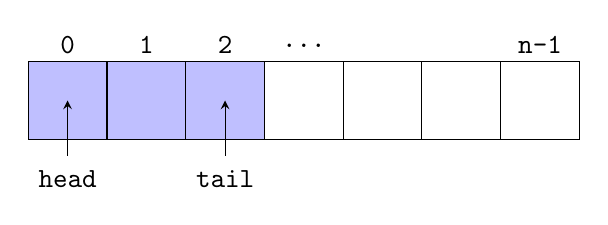
\begin{tikzpicture}
			[font=\ttfamily]
			\fill[blue, nearly transparent] (0,0) rectangle (3,-1);
			\draw (0,0) grid (7,-1);
			\node at (0.5,0.2) {0};
			\node at (1.5,0.2) {1};
			\node at (2.5,0.2) {2};
			\node at (3.5,0.2) {...};
			\node at (6.5,0.2) {n-1};
			\node at (2.5,-1.5) {tail};
			\node at (0.5,-1.5) {head};
			\draw [-stealth](0.5,-1.2) -- (0.5,-0.5);
			\draw [-stealth](2.5,-1.2) -- (2.5,-0.5);
		\end{tikzpicture}
	\captionof{figure}{Implementazione di una coda mediante array}
\end{minipage}\\
\begin{minipage}{.65\textwidth}
\centering
  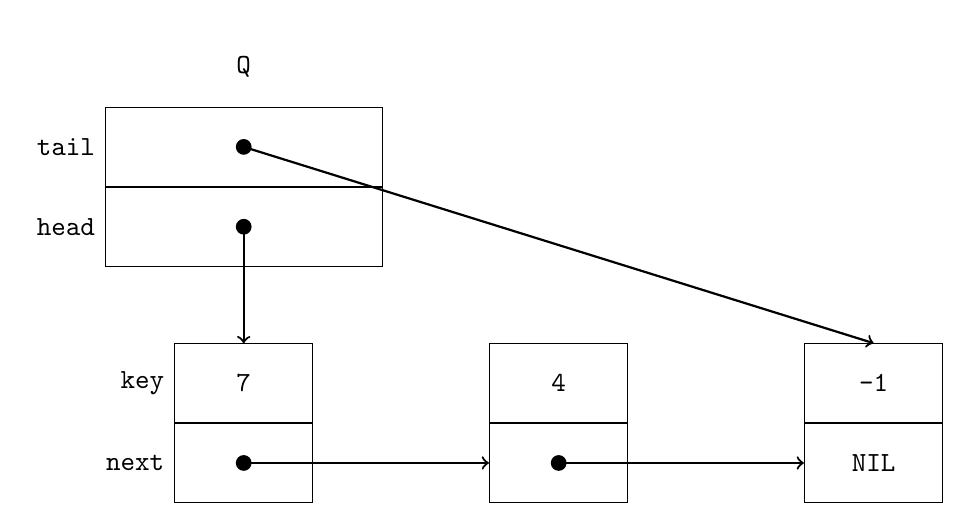
\begin{tikzpicture}[font=\ttfamily,minimum height=1cm,pointer/.style={fill, circle, minimum size=2mm, inner sep=0pt}]
	\node (tail) [rectangle,draw,minimum width=10em] {};
	\node (head) [rectangle,draw,anchor=north,minimum width=10em] at (tail.south) {};
	\node [anchor=south] at (tail.north) {Q};
	\node [anchor=east] at (tail.west) {tail};
	\node [anchor=east] at (head.west) {head};

	\node (a)[rectangle,draw,minimum width=5em] at (0,-3){7};
	\node (b)[rectangle,draw,anchor=north,minimum width=5em] at(a.south){};
	\node [anchor=east] at (a.west) {key};
	\node [anchor=east] at (b.west) {next};

	\node (c)[rectangle,draw,minimum width=5em] at (4,-3){4};
	\node (d)[rectangle,draw,anchor=north,minimum width=5em] at(c.south){};

	\node (e)[rectangle,draw,minimum width=5em] at (8,-3){-1};
	\node (f)[rectangle,draw,anchor=north,minimum width=5em] at(e.south){NIL};

	\draw[->,thick](tail.center) coordinate[pointer] -- (e.north);
	\draw[->,thick](head.center) coordinate[pointer] -- (a.north);
	\draw[->,thick](b.center) coordinate[pointer] -- (d.west);
	\draw[->,thick](d.center) coordinate[pointer] -- (f.west);
\end{tikzpicture}
\captionof{figure}{Implementazione di una coda mediante liste concatenate}
\end{minipage}
\end{center}

% Chapter 3: Strutture dati ramificate
\chapter{Strutture dati ramificate: gli alberi}
\section{Gli alberi}
\dfn{Albero radicato}{
Un albero è un insieme di elementi chiamati \textbf{nodi}, sui quali vengono definite relazioni di discendenza. Tra questi si distinguono gli \textbf{alberi radicati} nei quali uno dei vertici si distingue da tutti gli altri; questo vertice si chiama \textbf{radice} dell'albero.
}

Consideriamo un \textbf{nodo} $x$ in un albero radicato $T$ con radice $r$. Un nodo qualsiasi $y$ in un cammino semplice unico da $r$ a $x$ è detto \textbf{antenato} di $x$. Se $y$ è un antenato di $x$, allora $x$ è \textbf{discendente} di $y$. Se $y$ è un antenato di $x$ e $x\neq y$, allora $y$ è un \textbf{antenato proprio} di $x$ e $x$ è un \textbf{discendente proprio} di $y$. Il \textbf{sottoalbero con radice in $x$} è l'albero indotto dai discendenti di $x$, con radice in $x$.

Se l'ultimo arco nel cammino semplice dalla radice \textit{r} di un albero $T$ a un nodo \textit{x} è $(y,x)$, allora $y$ è il \textbf{padre} di \textit{x} e \textit{x} è un \textbf{figlio} di $y$. La radice è l'unico nodo in $T$ che non ha un padre. Se due nodi hanno lo stesso padre, sono \textbf{fratelli}. Un nodo senza figli è un \textbf{nodo esterno} o \textbf{foglia}. Un nodo non foglia è un \textbf{nodo interno}.

Il \textit{numero massimo di figli} che può avere un nodo $x$ in un albero radicato T è detto \textbf{grado} di $x$. La \textit{lunghezza} del cammino semplice dalla radice $r$ a un nodo $x$ è la \textbf{profondità} di $x$ in T. Un \textbf{livello} in un albero è costituito da tutti i nodi che stanno alla stessa profondità. Un livello si dice \textbf{saturo} se ogni suo nodo ha il massimo numero possibile di figli.

L'\textbf{altezza} di un nodo in un albero è il \textit{numero di archi nel più lungo cammino semplice che scende dal nodo a una foglia}; l'altezza di un albero è uguale alla profondità massima di un nodo qualsiasi dell'albero.
\begin{center}
\begin{forest}
for tree={
circle,
draw,
minimum size=.5cm,
fill=blue!25!white,
}
[R, name=root
[A
  [B]
  [C]
  [D]
]
[E
  [F]
  [G]
]
]
\end{forest}
\captionof{figure}{Un albero radicato con radice R e altezza 2}
\end{center}

\dfn{Albero ordinato}{
Un \textbf{albero ordinato} è un albero radicato in cui i figli di ogni nodo sono ordinati. Ovvero, se un nodo ha $k$ figli, allora c'è un primo figlio, un secondo figlio,$\ldots$, e un $k$-esimo figlio.
}
\subsection{Gli alberi binari}
\dfn{Albero binario}{
Un \textbf{albero binario} T è particolare tipo di albero in cui ogni nodo ha grado al più due. Ricorsivamente, un albero binario può essere costruito come segue:
\begin{enumerate}
\item un nodo \textbf{radice};
\item un albero binario detto \textbf{sottoalbero sinistro} della radice;
\item un albero binario detto \textbf{sottoalbero destro} della radice.
\end{enumerate}
}

\begin{center}
\begin{minipage}{.45\textwidth}
	\centering
		\begin{forest}
		for tree={
			circle,
			draw,
			minimum size=0.5cm,
			fill=blue!25!white,
		}
		[54, name=root
		[21
		[23
		[45]
		[67]
		]
		[34
		[12]
		[78]
		]
		]
		[45
		[67
		[89]
		[90]
		]
		[12
			[34]
			[45]
		]
		]
		]
	\end{forest}
	\captionof{figure}{Un albero binario pieno di altezza 3}
\end{minipage}
\begin{minipage}{.45\textwidth}
	\centering
	\begin{forest}
for tree={
circle,
draw,
minimum size=0.5cm,
fill=blue!25!white,
}
[54, name=root
[21
  [23
    [45]
    [67]
  ]
  [34
    [12]
    [78]
  ]
]
[45
  [67
    [89]
    [90]
  ]
  [12]
]
]
\end{forest}
\captionof{figure}{Un albero binario completo di altezza 3}\label{fig:binary_tree}
\end{minipage}
\end{center}

\subsubsection{Tipologie di alberi binari}
Tra le varie tipologie di alberi binari troviamo:
\begin{enumerate}
\item Alberi binari \textbf{pieni};
\item Alberi binari \textbf{completi}.
\end{enumerate}

\dfn{Albero binario pieno}{
Un albero binario si dice \textbf{pieno} se l'ultimo livello dell'albero è saturo.
}

\begin{osservation}
Per $n$ nodi un albero binario pieno ha l'altezza minima possibile.
\end{osservation}

\dfn{Albero binario completo}{
Un albero binario si dice \textbf{completo} se tutti i suoi nodi interni, tranne al più uno, hanno due figli e tutte le foglie sono a profondità $h$ o $h-1$, dove $h$ è l'altezza dell'albero.
}

\info{Osservazione}{
Un albero binario pieno è un albero completo ma non viceversa. L'albero mostrato in Figura~\ref{fig:binary_tree} è completo ma non pieno.
}

\subsubsection{Proprietà degli alberi binari}\label{alberi_binari_prop}
Gli alberi binari sono particolarmente interessanti perché godono delle seguenti proprietà che andremo a dimostrare:


\begin{propbox}
Un albero binario pieno di altezza $h$ ha $2^{h+1}-1$ nodi.
\end{propbox}
\begin{proof}
La prova è per induzione sull'altezza $h$.
\begin{enumerate}
	\item \textbf{Caso base} ($h=0$): un albero binario di altezza $h=0$ ha un solo nodo, la radice, e vale quindi:
	\begin{displaymath}
		2^{0+1}-1 = 1
	\end{displaymath}
Quindi il caso base è dimostrato.
\item \textbf{Passo induttivo} ($h > 1$): assumiamo per ipotesi induttiva che un albero binario completo di altezza $h$ abbia $2^{h+1}-1$ nodi, e dimostriamo che un albero binario $T$ completo di altezza $h+1$ ha $2^{(h+1)+1}-1=2^{h+2}-1$ nodi.

Come è fatto $T$? Ha la radice, più un sottoalbero sinistro $T_{s}$ e un sottoalbero destro $T_{d}$ entrambi completi e di altezza $h$. Per ipotesi induttiva quindi entrambi gli alberi $T_{s}$ e $T_{d}$ hanno rispettivamente $2^{h+1}-1$ nodi. Quindi il numero di nodi di $T$ sarà dato dalla somma dei nodi dei sottoalberi sinistro e destro e della sua radice. Detto $m$ il numero di nodi di $T$ abbiamo quindi:
\begin{displaymath}
	m = 1 + (2^{h+1}-1) + (2^{h+1}-1) = (2 \cdot 2^{h+1}) -1 = 2^{h+2}-1
\end{displaymath}
\end{enumerate}
\end{proof}


\begin{corolbox}
Un albero binario pieno di altezza $h$ ha esattamente $2^{h}$ foglie.
\end{corolbox}


\begin{propbox}
Sia $T$ un albero binario completo di altezza $h$. Allora il numero di nodi di $T$ è compreso tra $2^{h}$ e $2^{h+1}-1$.
\end{propbox}

\begin{proof}
Per dimostrare questo risultato abbiamo bisogno di determinare il numero massimo e minimo di nodi di un albero binario quasi completo di altezza $h$. Il numero massimo di nodi che un albero binario quasi completo di altezza $h$ può avere è pari al numero di nodi di albero binario completo di altezza $h$, ossia $max = 2^{h+1}-1$. Ora osserviamo che l’ albero binario quasi completo di altezza $h$ con numero minimo di nodi è illustrato in Figura \ref{fig:alberoquasicompleto} (dove $T_{s}$ e $T_{d}$ sono degli alberi binari completi di altezza $h-2$):
\begin{figure}[ht!]
\centering
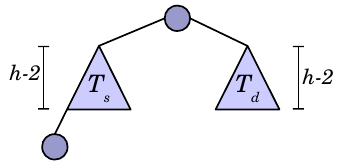
\includegraphics[scale=0.8]{res/Alberobinarioquasicompleto}
\caption{}\label{fig:alberoquasicompleto}
\end{figure}

Allora:
\begin{align*}
	\#_{nodi}(T) = 1+1+\#_{nodi}(T_{s})+\#_{nodi}(T_{d})
\end{align*}
dove:
\begin{align*}
\#_{nodi}(T_{s}) = \#_{nodi}(T_{d})=2^{h-1}-1
\end{align*}
Quindi:
\begin{align*}
\#_{nodi}(T) &= 2+(2^{h-1}-1)+(2^{h-1}-1)\\
&=2 \cdot 2^{h-1} \\
&= 2^{h}
\end{align*}

\end{proof}

\begin{propbox}
L'altezza di un albero binario completo $T$ con $n$ nodi è $h = \lfloor \log n \rfloor$.
\end{propbox}

\begin{proof}
Per la proposizione precedente abbiamo che $2^{h}\leq n \leq 2^{h+1}-1 < 2^{h+1}$, cioè, applicando i logaritmi, $h \leq \log n < h+1$ e quindi, applicando la funzione pavimento, $h \leq \lfloor \log n \rfloor<h+1$.Possiamo concludere che $h=\lfloor \log n \rfloor$.
\end{proof}

\subsection{Operazioni di visita in un albero binario}

\textbf{Visitare} un albero significa esaminare sequenzialmente tutti i suoi nodi. Le tipologie di visita si suddividono in due categorie: le \textbf{visite in profondità} e le \textbf{visite in ampiezza}.

\subsubsection{Visite in profondità}
Esistono tre tipi principali di visite in profondità:
\begin{enumerate}
	\item Nella \textbf{visita in ordine} si visita il sottoalbero sinistro, quindi si esamina la radice e infine si visita il sottoalbero destro;
	\begin{lstlisting}[language=asd,caption={Visita-InOrder(T)}]
	if T != nil then
		Visita-InOrder(T@\rightarrow@left)
		Visita(T)
		Visita-InOrder(T@\rightarrow@right)
	\end{lstlisting}
	\item Nella \textbf{visita in pre-ordine} si visita ricorsivamente prima la radice e quindi si visitano il sottoalbero sinistro e quello destro;
	\begin{lstlisting}[language=asd,caption={Visita-PreOrder(T)}]
	if T != nil then
		Visita(T)
		Visita-PreOrder(T@\rightarrow@left)
		Visita-PreOrder(T@\rightarrow@right)
	\end{lstlisting}

	\item Nella \textbf{visita in post-ordine} si visita ricorsivamente prima il sottoalbero sinistro, poi quello destro ed infine il nodo in radice.
	\begin{lstlisting}[language=asd,caption={Visita-PostOrder(T)}]
	if T != nil then
		Visita-PostOrder(T@\rightarrow@left)
		Visita-PostOrder(T@\rightarrow@right)
		Visita(T)
	\end{lstlisting}
\end{enumerate}

\begin{example}
	Dato l'albero binario:
	\begin{center}
		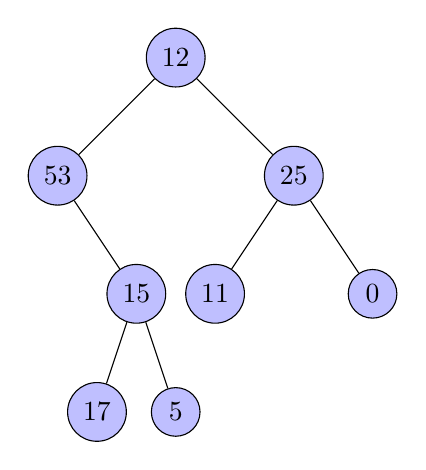
\begin{tikzpicture}
			[level 1/.style={sibling distance=3cm},
			level 2/.style={sibling distance=2cm},
			level 3/.style={sibling distance=1cm},
			every node/.style = {shape=circle, draw, align=center, fill=blue!25!white}]
			\node{12}
			child{
				node{53}
				child[missing]
				child{
					node{15}
					child{
						node{17}
					}
					child{
						node{5}
					}
				}
			}
			child{
				node{25}
				child{
					node{11}
				}
				child{
					node{0}
				}
			};
		\end{tikzpicture}
	\end{center}
	Supponiamo di avere un'operazione di visita che si occuperà di stampare la chiave conservata nel nodo correntemente visitato. Si avrà allora, per ciascuna tipologia di visita, il seguente output:
	\begin{enumerate}
		\item \textbf{Visita in PreOrder:} \texttt{12 53 15 17 5 25 11 0}
		\item \textbf{Visita in InOrder:} \texttt{53 17 15 5 12 11 25 0}
		\item \textbf{Visita in PostOrder:} \texttt{17 5 15 53 11 0 25 12}
	\end{enumerate}
\end{example}

\subsubsection{Visita in ampiezza}
Vediamo ora un altro tipo di visita chiamata \textbf{visita in ampiezza} (o \textbf{per livelli}).

L'idea della visita in ampiezza è quella di visitare dapprima la radice dell'albero, poi i figli della radice, poi i figli dei figli della radice e così via fino alle foglie.

In questo modo i nodi al livello $i$ saranno visitati solo dopo che tutti i nodi del livello $i-1$ sono stati visitati. La difficoltà che si incontra in questo tipo di visita è dato dal fatto che non esiste alcun collegamento tra i nodi di uno stesso livello.

Per questo motivo sarà necessario avvalersi di una \textit{struttura dati ausiliaria} dove inserire le informazioni sull'ordine dei nodi da visitare.

La struttura dati più adatta a questo scopo è la \textbf{coda}. Infatti, ogni volta che si visita un nodo, i suoi figli vengono inseriti in coda. In questo modo, quando si visita un nodo, si è sicuri che tutti i nodi di livello inferiore sono già stati visitati. L'algoritmo~\ref{lst:bfs_tree} mostra come implementare la visita in ampiezza.


\begin{example}
	Si consideri l'albero binario mostrato in Figura~\ref{fig:binary_Tree}. L'algoritmo di visita in ampiezza inizia visitando il nodo in radice che viene inserito in coda:

	\smallskip
	\begin{tblr}{hlines,vlines}
		1 \\
	\end{tblr}
	\smallskip

	La lettura avviene rimuovendo dalla coda l'elemento in testa, quindi il nodo in radice viene rimosso dalla coda e i suoi figli vengono inseriti in coda:
	\smallskip

	\begin{tblr}{hlines,vlines}
		3 & 2 \\
	\end{tblr}
	\smallskip

	Successivamente, il nodo 2 viene rimosso e si inseriscono in coda i suoi nodi figli:
	\smallskip

	\begin{tblr}{hlines,vlines}
		5 & 4 & 3 \\
	\end{tblr}
	\smallskip

	Una volta aver estratto il nodo 3 ed aver inserito i nodi figli, bisogna solo estrarre gli elementi in coda:
	\smallskip

	\begin{tblr}{hlines,vlines}
		7 & 6 & 5 & 4 \\
	\end{tblr}
	\smallskip

	In questo modo la lettura dell'albero in ampiezza produce il seguente output: \texttt{1 2 3 4 5 6 7}
	\begin{center}
		\begin{forest}
			for tree={
				circle,
				draw,
				minimum size=0.7cm,
				fill=blue!25!white,
			}
			[1
			[2
			[4]
			[5]
			]
			[3
			[6]
			[7]
			]
			]
		\end{forest}
		\captionof{figure}{}\label{fig:binary_Tree}
	\end{center}

\end{example}


\begin{lstlisting}[language=asd,label=lst:bfs_tree,caption={BFS(T)}]
// Accodiamo la testa dell'albero
Q = {T}
while Q @\neq@ {} do
	// Leggo la testa della coda
	x = Head(Q)
	Visita(x)
	// Accodo i figli sinistro e destro
	Q = Enqueue(Q, x@\rightarrow@ left)
	Q = Enqueue(Q, x@\rightarrow@ right)
	// Decodo
	Q = Dequeue(Q)
\end{lstlisting}

\section{Alberi binari di ricerca}
Finora abbiamo esplorato le proprietà algebriche delle strutture dati, ma ora ci concentreremo su un tipo particolare di struttura: gli Alberi Binari di Ricerca (ABR). Prima di addentrarci in questo argomento, vale la pena fare un confronto con le strutture dati lineari che abbiamo precedentemente studiato.

Le strutture dati lineari, come le liste, gli array e le code, organizzano i dati in una sequenza unidimensionale, simile a una fila di oggetti allineati in una vetrina. Queste strutture sono efficaci per molte applicazioni, ma possono avere limitazioni quando si tratta di ricerche efficienti o di mantenere un ordine specifico dei dati.

Gli \textbf{alberi binari di ricerca}, al contrario, sfruttando la proprietà \ref{prop:abr} offre vantaggi distinti, in particolare nella ricerca rapida e nell'ordinamento automatico dei dati come si vedrà nei paragrafi successivi.


\begin{axiombox}{Proprietà di ordinamento degli alberi binari di ricerca}\label{prop:abr}
Sia $x$ un nodo in un albero \textsc{ABR}. Se $y$ è un nodo nel sottoalbero sinistro di $x$, allora $y.key \leq x.key$. Se $y$ è un nodo nel sottoalbero destro di $x$, allora $y.key \geq x.key$. In altre parole, i valori più piccoli sono sempre a sinistra e i valori più grandi sono sempre a destra.
\end{axiombox}


\begin{example}
	Si osservi l'albero binario di ricerca in Figura~\ref{fig:binary_search_tree}. In questo albero, per ogni nodo $x$, le chiavi di tutti i nodi nel sottoalbero sinistro di $x$ sono minori o uguali a $x.key$, e le chiavi di tutti i nodi nel sottoalbero destro di $x$ sono maggiori o uguali a $x.key$.

\begin{center}
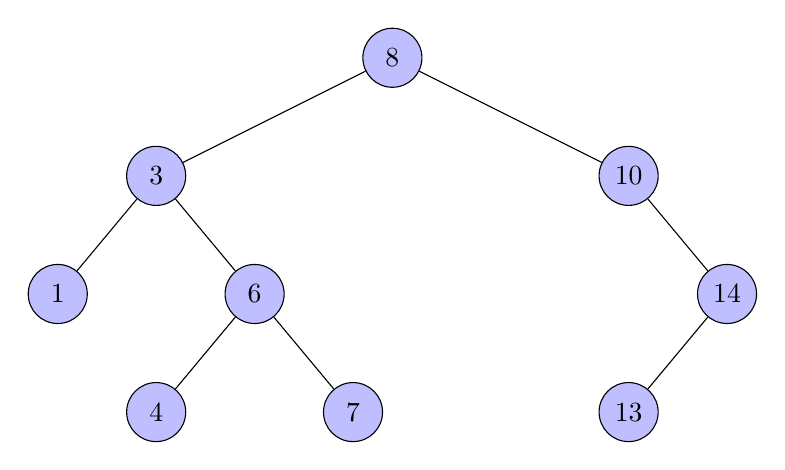
\begin{tikzpicture}
[every node/.style={draw,circle,minimum size=.75cm,fill=blue!25!white},
level 1/.style={sibling distance=6cm},
level 2/.style={sibling distance=2.5cm},
level 3/.style={sibling distance=2.5cm}]
\node{8}
child{
node{3}
child{
  node{1}
}
child{
  node{6}
  child{
    node{4}
  }
  child{
    node{7}
  }
}
}
child{
node{10}
child[missing]
child{
  node{14}
  child{
    node{13}
  }
  child[missing]
}
};
\end{tikzpicture}
\captionof{figure}{Esempio di albero binario di ricerca}\label{fig:binary_search_tree}
\end{center}
\end{example}

Dalla proprietà degli alberi \textsc{ABR} si può dedurre che per ogni albero di ricerca T, sia il sottoalbero sinistro che quello destro sono alberi binari di ricerca. È possibile quindi definire induttivamente un albero binario di ricerca:
\begin{displaymath}
T=
\begin{cases}
\varnothing & \mbox{se vuoto}\\
\begin{cases}
  \text{un sottoalbero \textsc{abr} sinistro }T_{1} \land \ \forall y \in T_{1}(y.key \leq root.key)  \\
  \text{un sottoalbero \textsc{abr} destro }T_{2} \land \ \forall y \in T_{2} (y.key \geq root.key)
\end{cases}
& \mbox{altrimenti}
\end{cases}
\end{displaymath}

\subsection{Operazioni di ricerca}

\subsubsection{Ricerca di un elemento}
Supponiamo di avere un albero binario di ricerca $T$ e si voglia implementare un algoritmo \textsc{Search} che verifichi se un elemento $k$ appartiene all'albero. Sfruttando la proprietà dell'albero \textsc{abr} basterà effettuare un controllo tra $k$ e la chiave memorizzata nel nodo in radice.
\begin{itemize}
\item Se $x.key=k$ abbiamo trovato l'elemento;
\item Se $k < x.key$ allora bisogna cercare
$k$ nel sottoalbero sinistro;
\item Se $k > x.key$ allora bisogna cercare $k$ nel sottoalbero destro.
\end{itemize}
Si ottiene quindi l'algoritmo~\ref{lst:search} molto simile alla ricerca binaria all'interno di un array ordinato. La differenza è che, mentre la ricerca binaria divide l'array in due parti uguali, la ricerca in un albero binario di ricerca divide l'albero in due sottoalberi che possono avere dimensioni molto diverse. Il numero massimo di confronti nel caso peggiore sarà infatti pari alla lunghezza del percorso più lungo, quindi il tempo di esecuzione sarà pari all'altezza dell'albero.

\begin{lstlisting}[language=asd,caption={Search(T,k)},label=lst:search]
if T @\neq@ NIL then
	if T@\rightarrow@key < k then
  		return Search(T@\rightarrow@right, k)
	else if T@\rightarrow@key > k then
  		return Search(T@\rightarrow@left, k)
	else
  		return T
\end{lstlisting}

\subsubsection{Ricerca del minimo e del massimo}
La ricerca del minimo e del massimo sono operazioni banali in un albero binario di ricerca grazie al vincolo di ordinamento globale che questi offrono. Infatti il minimo e il massimo si troveranno sempre nel \textit{nodo più a sinistra e nel nodo più a destra}, rispettivamente.

Ne consegue che il costo della ricerca sarà \textbf{lineare sull'altezza dell'albero} dato che sarà necessario seguire un percorso dalla radice fino a una foglia.

Più precisamente, il minimo si troverà sempre lungo il ramo più a sinistra dell'albero e sarà caratterizzato dal fatto di non avere un figlio sinistro. Dualmente, il massimo sarà il primo nodo del percorso estremo destro che non ha un figlio destro.

\begin{center}
\begin{minipage}{.45\textwidth}

\begin{lstlisting}[language=asd,caption={Search-Min(T)},label=lst:search_min]
	ret = T
	if T @\neq@ NIL then
		x = Search-Min(T@\rightarrow@left)
	if x @\neq@ NIL then
		ret = x
	return ret
\end{lstlisting}
\end{minipage}
\begin{minipage}{.45\textwidth}
	\begin{lstlisting}[language=asd,caption={Search-Max(T)},label=lst:search_max]
	ret = T
	if T @\neq@ NIL then
		x = Search-Max(T@\rightarrow@right)
	if x @\neq@ NIL then
		ret = x
	return ret
\end{lstlisting}
\end{minipage}
\end{center}

\subsubsection{Ricerca del successore e del predecessore}
Dato un nodo in un albero binario di ricerca, a volte è importante trovare il suo successore nell'ordine stabilito da un attraversamento simmetrico. Se tutte le chiavi sono distinte, il successore di un nodo $x$ è il nodo con la chiave più piccola che è maggiore di $x.key$.

La struttura di un albero binario di ricerca consente di determinare il successore di un nodo senza mai dover confrontare le chiavi.

L'algoritmo \textsc{Search-Succ}$(T,k)$ verifica se l'albero $T$ è vuoto, altrimenti si aprono tre strade:
\begin{itemize}
	\item $x.key < k$: la radice contiene un valore minore della chiave, quindi se il successore esiste sarà a destra del nodo $x$, ovvero proprio il risultato che darà la chiamata \textsc{Search-Succ}$(T \rightarrow right, k)$;
	\item $x.key > k$: il successore sarà il risultato della chiamata \textsc{Search-Succ}$(T \rightarrow left,k)$, se $T\rightarrow left = \varnothing$ allora il successore sarà proprio il nodo $x$ (a destra avrò solo valori maggiori di $x$ quindi già so che il miglior candidato è $x$ stesso).
	\item $x.key = k$: è evidente che collassa al caso $x.key<k$, poiché se il successore esiste sarà nel sottoalbero destro.
\end{itemize}

\begin{lstlisting}[language=asd,caption={Search-Succ(T,k)},label=lst:search_succ]
	if T @\neq@ NIL then
		if T@\rightarrow@key @\leq@ k then
			return Search-Succ(T@\rightarrow@right, k)
		else
			x = Search-Succ(T@\rightarrow@left, k)
		if x = NIL then
			return T
		else
			return x
\end{lstlisting}

\subsection{Operazioni di modifica}

\subsubsection{Inserimento di un elemento}
Supponiamo di voler inserire un nodo $x$ di chiave $k$ in un albero $T$. L'operazione di inserimento consiste nell'ottenere un nuovo albero, detto $T'$, posto in questo modo:
\begin{displaymath}
T'= T \cup \{x\}
\end{displaymath}
Supposto che non debbano esserci chiavi duplicate, esistono due casi possibili:
\begin{enumerate}
\item \textbf{L'albero iniziale è vuoto}, quindi basta effettuare un inserimento in testa
\item \textbf{L'albero iniziale non è vuoto}, quindi $x$ deve essere inserito nel sottoalbero vuoto corretto. Infatti, se $x \notin T$, allora inserirlo in $T$ significa cercare un sottoalbero vuoto (o alla peggio una foglia) che soddisfa la proprietà dell'ordinamento.
\end{enumerate}

\begin{lstlisting}[language=asd,caption={Insert(T,k)},label=lst:insert_bst]
if T = NIL then
	x = Alloca()
	x@\rightarrow@key = k
	x@\rightarrow@left = x@\rightarrow@right = NIL
	T = x
else if T@\rightarrow@key < k then
	Insert(T@\rightarrow@right, k)
else
	Insert(T@\rightarrow@left, k)
\end{lstlisting}

\begin{example}
Consideriamo l'albero \ref{fig:binary_search_tree} e supponiamo di voler inserire il nodo 5. L'algoritmo \ref{lst:insert_bst} controlla innanzitutto che l'albero non sia vuoto, successivamente confronta il dato 5 con le varie radici per capire in quale sottoalbero deve richiamarsi. Una volta arrivato al nodo 4, l'algoritmo arriva al caso base ed effettua l'inserimento di un nuovo nodo.
\begin{center}
		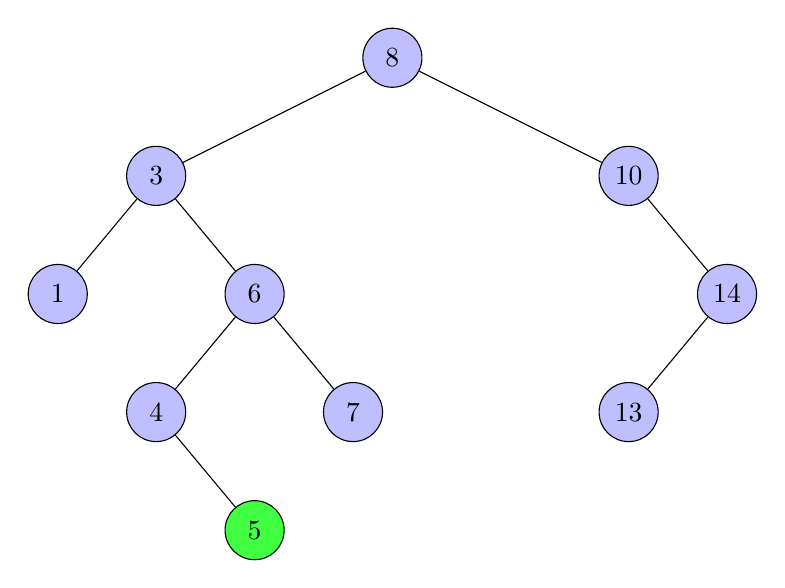
\begin{tikzpicture}
			[every node/.style={draw,circle,minimum size=.75cm,fill=blue!25!white},
			level 1/.style={sibling distance=6cm},
			level 2/.style={sibling distance=2.5cm},
			level 3/.style={sibling distance=2.5cm}]
			\node{8}
			child{
				node{3}
				child{
					node{1}
				}
				child{
					node{6}
					child{
						node{4}
						child[missing]
						child{
							node[fill=green!75!white]{5}
						}
					}
					child{
						node{7}
					}
				}
			}
			child{
				node{10}
				child[missing]
				child{
					node{14}
					child{
						node{13}
					}
					child[missing]
				}
			};
		\end{tikzpicture}
	\captionof{figure}{Esempio di inserimento in un albero binario di ricerca}
\end{center}
\end{example}

\subsubsection{Cancellazione di un nodo}\label{sez:abr_delete}
\paragraph{Eliminiazione di una foglia}
Consideriamo l'albero binario di ricerca mostrato in Figura~\ref{fig:delete-abr-1}. Supponiamo di voler cancellare il nodo con chiave 5. In questo caso il nodo da eliminare non ha figli e possiamo cancellarlo semplicemente impostando il puntatore \texttt{right} del padre a \textsc{nil}. Questo è il caso più semplice di \hypertarget{abr:delete}{cancellazione}.

\begin{center}
\begin{minipage}{.45\textwidth}
\centering
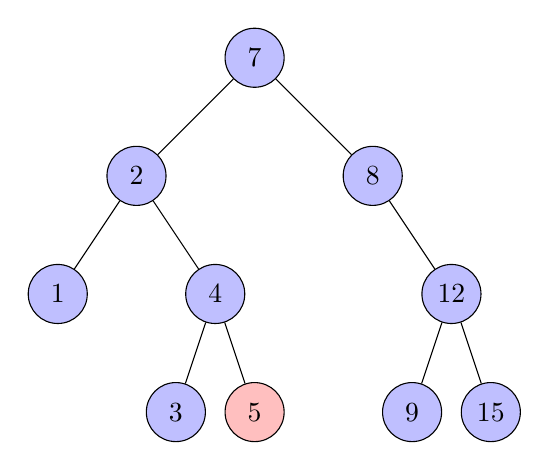
\begin{tikzpicture}
[every node/.style={draw,circle,minimum size=.75cm,fill=blue!25!white},
level 1/.style={sibling distance=3cm},
level 2/.style={sibling distance=2cm},
level 3/.style={sibling distance=1cm}]
\node{7}
child{
node{2}
child{
node{1}
}
child{
node{4}
child{
  node{3}
}
child{
  node[fill=red!25!white]{5}
}
}
}
child{
node{8}
child[missing]
child{
  node{12}
  child{
    node{9}
  }
  child{
    node{15}
  }
}
};
\end{tikzpicture}
\captionof{figure}{Cancellazione in un albero binario di ricerca: caso 1}\label{fig:delete-abr-1}
\end{minipage}
\hfil
\begin{minipage}{.45\textwidth}
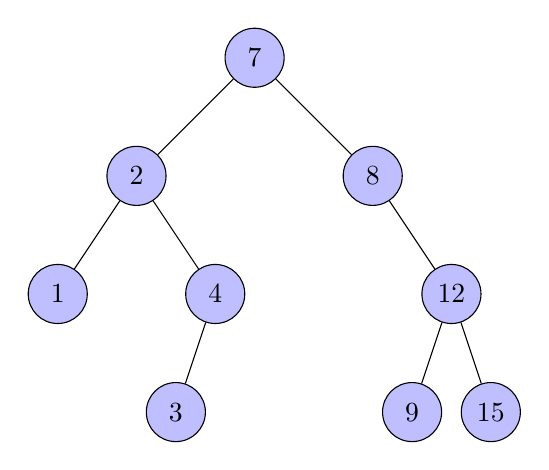
\begin{tikzpicture}
[every node/.style={draw,circle,minimum size=.75cm,fill=blue!25!white},
level 1/.style={sibling distance=3cm},
level 2/.style={sibling distance=2cm},
level 3/.style={sibling distance=1cm}]
\node{7}
child{
node{2}
child{
node{1}
}
child{
node{4}
child{
  node{3}
}
child[missing]
}
}
child{
node{8}
child[missing]
child{
  node{12}
  child{
    node{9}
  }
  child{
    node{15}
  }
}
};
\end{tikzpicture}
\captionof{figure}{Albero risultante dalla cancellazione}\label{fig:delete-abr-1-result}
\end{minipage}
\end{center}
\paragraph{Eliminazione di un nodo con un solo figlio}
Consideriamo ora il caso in cui il nodo da eliminare abbia un solo figlio come nel caso del nodo con chiave 4 mostrato in Figura~\ref{fig:delete-abr-2}. In questa situazione si procede eliminando il nodo e collegando il padre del nodo da eliminare con il figlio del nodo da eliminare. Nel caso in cui il nodo da eliminare sia la radice, allora il figlio del nodo da eliminare diventa la nuova radice dell'albero. (Figura~\ref{fig:delete-abr-2-result})

\begin{center}
\begin{minipage}{.45\textwidth}
\centering

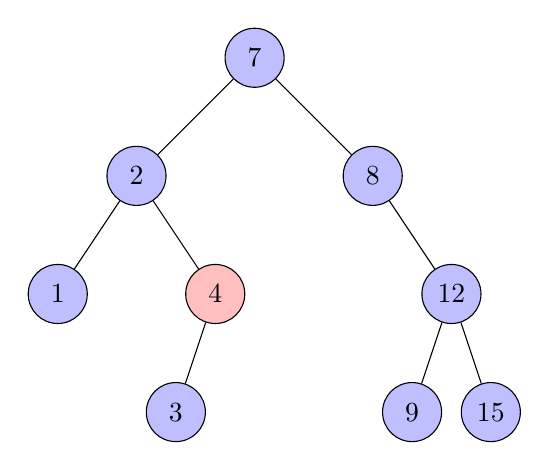
\begin{tikzpicture}
[every node/.style={draw,circle,minimum size=.75cm,fill=blue!25!white},
level 1/.style={sibling distance=3cm},
level 2/.style={sibling distance=2cm},
level 3/.style={sibling distance=1cm}]
\node{7}
child{
node{2}
child{
node{1}
}
child{
node[fill=red!25!white]{4}
child{
  node{3}
}
child[missing]
}
}
child{
node{8}
child[missing]
child{
  node{12}
  child{
    node{9}
  }
  child{
    node{15}
  }
}
};
\end{tikzpicture}
\captionof{figure}{Cancellazione in un albero binario di ricerca: caso 2}\label{fig:delete-abr-2}
\end{minipage}
\begin{minipage}{.45\textwidth}
\centering
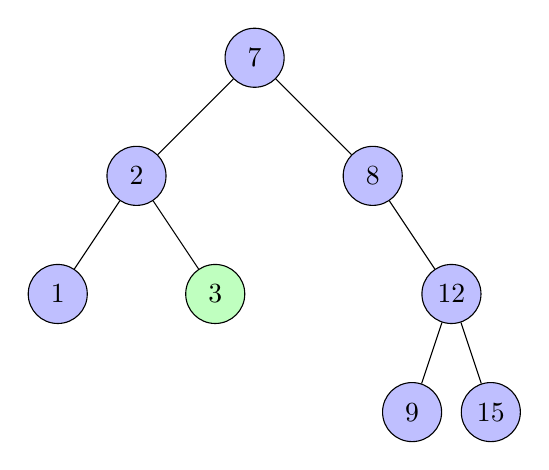
\begin{tikzpicture}
[every node/.style={draw,circle,minimum size=.75cm,fill=blue!25!white},
level 1/.style={sibling distance=3cm},
level 2/.style={sibling distance=2cm},
level 3/.style={sibling distance=1cm}]
	\node{7}
	child{
		node{2}
		child{
			node{1}
		}
		child{
			node[fill=green!25!white]{3}
		}
	}
	child{
		node{8}
		child[missing]
		child{
			node{12}
			child{
				node{9}
			}
			child{
				node{15}
			}
		}
	};
\end{tikzpicture}
\captionof{figure}{Albero risultante dalla cancellazione}\label{fig:delete-abr-2-result}
\end{minipage}
\end{center}
\paragraph{Eliminazione di un nodo con due figli}
Il caso più complesso è quello in cui il nodo da eliminare ha due figli. Per esempio, consideriamo la cancellazione del nodo con chiave 2 all'interno del albero binario di ricerca mostrato in Figura~\ref{fig:delete-abr-3}. In questo caso è necessario trovare il \textbf{successore del nodo da eliminare}, ovvero il nodo con la chiave più piccola nel sottoalbero destro del nodo da eliminare che nel nostro caso è rappresentato dal nodo di chiave 3 (Figura~\ref{fig:delete-abr-3-min}).

Il successore è garantito essere privo di figlio sinistro\footnote{Se così non fosse allora esisterebbe un nodo con chiave minore}, quindi può essere eliminato usando uno dei due casi precedenti. La ricerca del successore si ricondurrà quindi alla ricerca del nodo minimo all'interno del sottoalbero destro del nodo da eliminare. Una volta trovato questo minimo sarà sufficiente \textbf{staccarlo} (Figura \ref{fig:delete-abr-3-min-detach}) dalla sua posizione attuale e sostituirlo al nodo da eliminare. Gli eventuali figli destri del successore verranno poi attaccati al padre. (Figura~\ref{fig:delete-abr-3-result})

Per questo motivo sarà necessario definire tre algoritmi: \textsc{Cancella}$(T,k)$, \textsc{Cancella-Radice}$(T)$ e \textsc{Stacca-Minimo}$(T)$. L'algoritmo \textsc{Cancella}$(T,k)$ è l'algoritmo principale che si occupa di cancellare un nodo $k$ dall'albero $T$. Sulla base dei confronti si determina il percorso da seguire fino a quando non si arriva al nodo da eliminare, sarà poi compito dell'algoritmo \textsc{Delete-Root}$(T)$ di discriminare i casi appena descritti.

\begin{lstlisting}[language=asd,caption={\textsc{Cancella}(T,k)},label=lst:delete]
if T @\neq@ NIL then
	if T@\rightarrow@key < k then
		T@\rightarrow@left = Cancella(T@\rightarrow@left, k)					//Cancellazione nel sottoalbero sx
	else if T@\rightarrow@key > k then
		T@\rightarrow@right = Cancella(T@\rightarrow@right, k)			//Cancellazione nel sottoalbero dx
	else
		T = Delete-Root(T)				    //Cancellazione in radice
return T
\end{lstlisting}

Nel caso in cui $T$ abbia un solo figlio basterà aggiornare $T$ con l'indirizzo del figlio e deallocare la vecchia radice.  Qualora invece il nodo in radice avesse due figli sarà l'algoritmo \textsc{Stacca-Minimo}$(T,P)$ ad occuparsi di staccare il minimo del sottoalbero destro del nodo da eliminare. Il parametro $P$ serve per ricordarsi il padre di $T$ durante la discesa.

\begin{lstlisting}[language=asd,caption={\textsc{Delete-Root}(T)},label=lst:delete-root]
if T @\neq@NIL then
// Caso 1: T ha due figli
if T@$\rightarrow$@ left  @$\neq$@ NIL && T@$\rightarrow$@ right  @$\neq$@ NIL then
 	tmp = Stacca-Minimo(T@$\rightarrow$@ right,T)
 	T @$\rightarrow$@ key = tmp
else
// Caso 2: T ha un solo figlio
 	tmp = T
 	if T@$\rightarrow$@ right @$\neq$@ NIL then
 		T = T @$\rightarrow$@  right
 	else
 		T = T@$\rightarrow$@ left
 	Dealloca(tmp)
return T
\end{lstlisting}

\marker{yellow!50}{yellow!20!black}{\textsc{Stacca-Minimo} non fa altro che restituire la chiave del nodo minimo presente nel sottoalbero sinistro in modo tale da eseguire una sovrascrittura delle chiavi. Dopo di che, aggiorna i puntatori del nodo padre in modo tale che questo venga allacciato ai nodi restanti del sottoalbero destro.}

\begin{lstlisting}[language=asd,caption={\textsc{Stacca-Minimo}(T,P)},label=lst:delete-min]
if T@\neq@NIL then
	//Caso base: T ha un figlio sinistro
	if T@\rightarrow@left @\neq@ NIL then
		return Stacca-Minimo(T@\rightarrow@left, T)
	else
		tmp = T@$\rightarrow$@ key
		// Aggiorno i puntatori del padre
		// Caso 1: T era figlio sinistro del padre
		if P @\rightarrow@left = T then
		  P@\rightarrow@left = T@\rightarrow@right
		// Caso 2: T era figlio destro del padre
		else
		  P@\rightarrow@right = T@\rightarrow@right
		return tmp
\end{lstlisting}

\begin{center}
\begin{minipage}{.45\textwidth}
\centering
	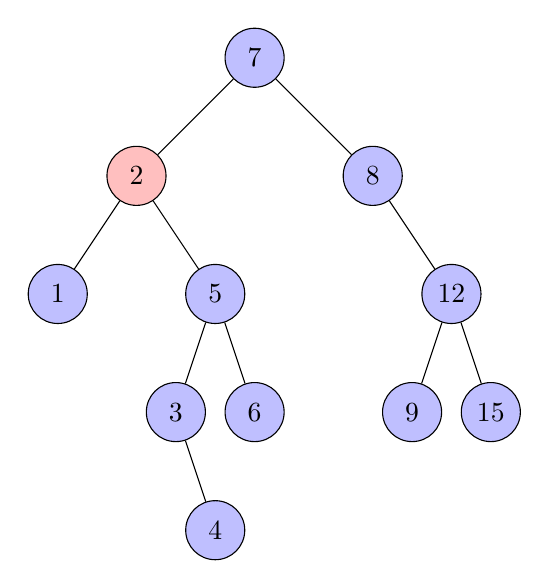
\begin{tikzpicture}
		[every node/.style={draw,circle,minimum size=.75cm,fill=blue!25!white},
		level 1/.style={sibling distance=3cm},
		level 2/.style={sibling distance=2cm},
		level 3/.style={sibling distance=1cm}]
		\node{7}
		child{
			node[fill=red!25!white]{2}
			child{
				node{1}
			}
			child{
				node{5}
				child{
					node{3}
					child[missing]
					child{
						node{4}
					}
				}
				child{
					node{6}
				}
			}
		}
		child{
			node{8}
			child[missing]
			child{
				node{12}
				child{
					node{9}
				}
				child{
					node{15}
				}
			}
		};
	\end{tikzpicture}
	\captionof{figure}{Cancellazione in un albero binario di ricerca: caso 3}\label{fig:delete-abr-3}
\end{minipage}
\begin{minipage}{.45\textwidth}
	\centering
	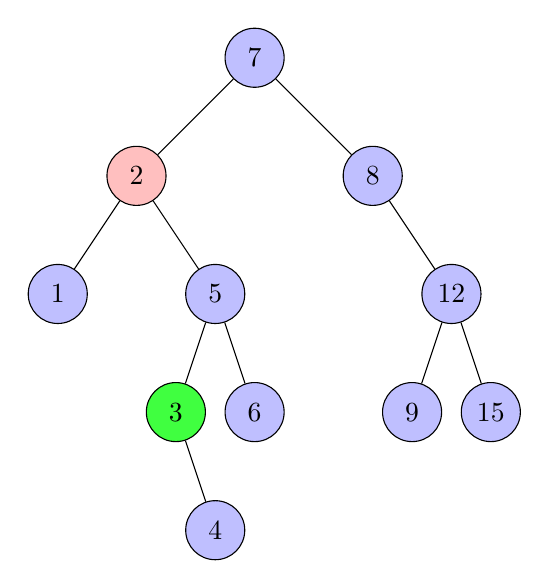
\begin{tikzpicture}
		[every node/.style={draw,circle,minimum size=.75cm,fill=blue!25!white},
		level 1/.style={sibling distance=3cm},
		level 2/.style={sibling distance=2cm},
		level 3/.style={sibling distance=1cm}]
		\node{7}
		child{
			node[fill=red!25!white]{2}
			child{
				node{1}
			}
			child{
				node{5}
				child{
					node[fill=green!75!white]{3}
					child[missing]
					child{
						node{4}
					}
				}
				child{
					node{6}
				}
			}
		}
		child{
			node{8}
			child[missing]
			child{
				node{12}
				child{
					node{9}
				}
				child{
					node{15}
				}
			}
		};
	\end{tikzpicture}
	\captionof{figure}{Individuazione del successore del nodo da eliminare}\label{fig:delete-abr-3-min}
\end{minipage}
\begin{minipage}{.45\textwidth}
\centering
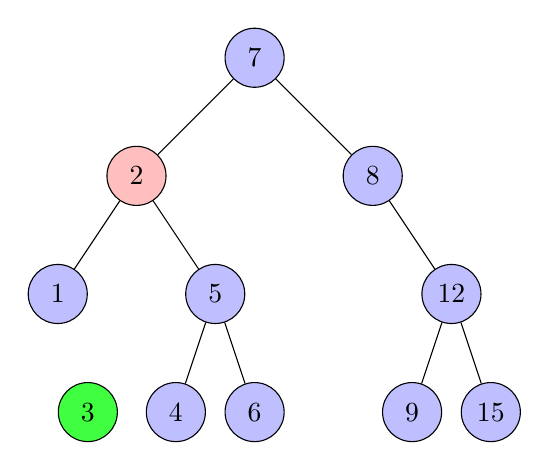
\begin{tikzpicture}
	[every node/.style={draw,circle,minimum size=.75cm,fill=blue!25!white},
	level 1/.style={sibling distance=3cm},
	level 2/.style={sibling distance=2cm},
	level 3/.style={sibling distance=1cm}]
	\node{7}
	child{
		node[fill=red!25!white]{2}
		child{
			node{1}
		}
		child{
			node{5}
			child{
				node[name=4]{4}
			}
			child{
				node{6}
			}
		}
	}
	child{
		node{8}
		child[missing]
		child{
			node{12}
			child{
				node{9}
			}
			child{
				node{15}
			}
		}
	};
	\node[shape=circle, draw, align=center, fill=green!75!white] at ([xshift=-1.5cm]4.east) {3};
\end{tikzpicture}
\captionof{figure}{Staccaggio del successore}\label{fig:delete-abr-3-min-detach}
\end{minipage}
\begin{minipage}{.45\textwidth}
\centering
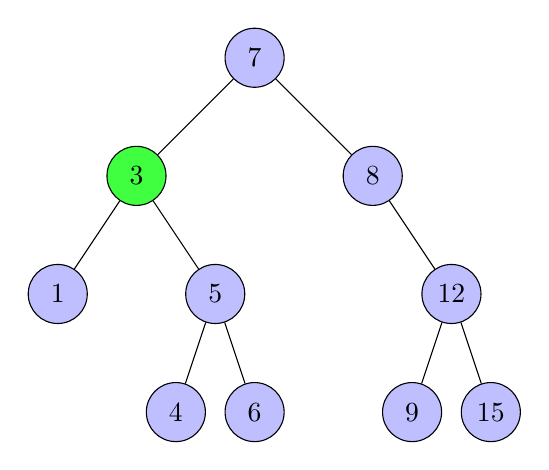
\begin{tikzpicture}
	[every node/.style={draw,circle,minimum size=.75cm,fill=blue!25!white},
	level 1/.style={sibling distance=3cm},
	level 2/.style={sibling distance=2cm},
	level 3/.style={sibling distance=1cm}]
	\node{7}
	child{
		node[fill=green!75!white]{3}
		child{
			node{1}
		}
		child{
			node{5}
			child{
				node{4}
			}
			child{
				node{6}
			}
		}
	}
	child{
		node{8}
		child[missing]
		child{
			node{12}
			child{
				node{9}
			}
			child{
				node{15}
			}
		}
	};
\end{tikzpicture}
\captionof{figure}{Albero risultante dalla cancellazione}\label{fig:delete-abr-3-result}
\end{minipage}
\end{center}

\section{Alberi AVL}
\subsection{Alberi bilanciati}
Gli alberi bilanciati di ricerca sorgono come una soluzione ai problemi di inefficienza che possono emergere negli alberi binari di ricerca. Infatti, la creazione di un albero binario di ricerca non bilanciato, in cui un sottoalbero ha molte più profondità rispetto all'altro, può portare a un'operazione di ricerca con una complessità temporale peggiorativa, che può diventare lineare rispetto al numero di elementi nell'albero. Questo è chiaramente inaccettabile in applicazioni in cui è necessaria una risposta rapida.

Gli \textbf{alberi bilanciati di ricerca} affrontano questo problema stabilendo rigorosi vincoli sulla loro struttura capaci di garantire un buon bilanciamento tra le altezze dei sottoalberi sinistro e destro di ciascun nodo. Questo bilanciamento delle altezze è ottenuto mediante regole di inserimento e rimozione particolari, e il risultato è un albero in cui le operazioni di ricerca, inserimento e cancellazione hanno una complessità temporale tipicamente logaritmica, garantendo prestazioni prevedibili e ottimali in qualsiasi scenario. Nelle prossime sezioni esploreremo le specifiche regole e le varianti di alberi bilanciati di ricerca, come gli alberi AVL e gli alberi rosso-neri per comprendere appieno come questi vincoli migliorino notevolmente l'efficienza delle operazioni sugli alberi binari di ricerca.

\dfn{Alberi bilanciati di ricerca}{
Una classe di alberi binari di ricerca si dice \textbf{bilanciata} se
\begin{displaymath}
	h(T) = \Theta(\log_{2}n) \qquad \mbox{dove } n = |T| \ \mbox{è la cardinalità di T}
\end{displaymath}
}


\begin{osservation}
Gli alberi binari completi appartengono alla classe degli alberi bilanciati.
\end{osservation}

Un'altra classe di alberi binari che soddisfa alle nostre esigenze è quella degli \textbf{alberi perfettamente bilanciati}.

\dfn{Alberi perfettamente bilanciati}{
Un albero binario di ricerca T si dice \textbf{perfettamente bilanciato} (\textbf{APB}) se:
\begin{equation}
	\forall x \in T \qquad ||x \rightarrow left| - |x\rightarrow right||\leq 1
\end{equation}
ovvero la differenza, per ogni nodo di $T$, in valore assoluto tra la cardinalità del sottoalbero sinistro e quello destro è al più uno.
}
\begin{example}
L'albero binario di ricerca in Figura~\ref{fig:perfectly_balanced_tree} è perfettamente bilanciato, infatti per ogni nodo la differenza tra il numero di nodi nel sottoalbero sinistro e destro è al più uno. Preso ad esempio il nodo in radice, la differenza tra i suoi due sottoalberi è:
\begin{displaymath}
| |root \rightarrow left| - |root \rightarrow right||=|2 - 3 | = |-1|=1 \leq 1
\end{displaymath}

Gli alberi perfettamente bilanciati riescono a garantire un tempo di esecuzione logaritmico per le operazioni di ricerca, inserimento e cancellazione. Tuttavia, questa classe di alberi è molto restrittiva, poiché richiede numerosi controlli a fronte di ogni inserimento o cancellazione. Per questo motivo, gli alberi perfettamente bilanciati non sono molto utilizzati in pratica.
\end{example}

\begin{center}
\begin{minipage}{.45\textwidth}
	\centering
	\begin{forest}
	for tree={
		circle,
		draw,
		minimum size=0.5cm,
		fill=blue!25!white,
	}
	[
	[
	[ ]
	[ ]
	]
	[
	[
	[,phantom]
	[]
	]
	[]
	]
	]
\end{forest}
\captionof{figure}{Esempio di albero perfettamente bilanciato}\label{fig:perfectly_balanced_tree}
\end{minipage}
\begin{minipage}{.45\textwidth}
	\centering
	\begin{forest}
		for tree={
			circle,
			draw,
			minimum size=0.5cm,
			fill=blue!25!white,
		}
		[
			[
				[]
				[]
			]
			[]
		]
	\end{forest}
	\captionof{figure}{Esempio di albero non perfettamente bilanciato}\label{fig:not_perfectly_balanced_tree}
\end{minipage}
\end{center}

\subsection{Gli alberi AVL}
La classe di alberi \textbf{AVL (Adelson-Velskii e Landis)} rappresenta una classe di alberi bilanciati con buone prestazioni e gestione relativamente semplice. È praticamente una versione più permissiva di \textsc{APB}.

\dfn{Alberi AVL}{
Un albero $T$ è \textsc{avl} se e solo se:
\begin{equation}\label{avl_prop}
	\forall x \in T \qquad |h(x \rightarrow left) -h(x \rightarrow right)|\leq 1
\end{equation}
ovvero se, per ogni nodo dell'albero, la differenza in modulo dell'altezza del sottoalbero sinistro e il sottoalbero destro è al più uno.
}

Analogamente a quanto visto per le strutture dati precedenti, è possibile definire un albero AVL in modo ricorsivo: un albero binario di ricerca $T$ appartiene alla classe \textsc{AVL} se e soltanto se la differenza tra l'altezza del suo sottoalbero destro e il suo sottoalbero sinistro è minore o uguale di uno e i due sottoalberi appartengono alla classe \textsc{AVL}.

La variabilità negli alberi \textsc{avl} è abbastanza ampia, infatti con lo stesso numero di nodi è possibile generare molti alberi \textsc{avl}. Ma la cosa interessante è che \textbf{ogni albero perfettamente bilanciato è \textsc{avl}} poiché è di fatto un albero completo, il quale rispetta la proprietà di AVL per definizione.

Nel caso degli AVL però non possiamo immediatamente definire una relazione tra l’altezza e il numero dei nodi (con $n$ nodi possiamo infatti generare diversi \textsc{avl} con altezza differente). Per raggiungere il nostro obiettivo dobbiamo restringere la classe \textsc{avl} in una particolare sottoclasse così da far valere la proprietà per tutti gli \textsc{avl}.

Generalmente, una proprietà valida per una sottoclasse non si estende alla superclasse, ma noi andremo a prendere degli alberi AVL con altezza peggiore possibile ed è intuitivo pensare che se per gli alberi peggiori vale $O(\log n)$ allora anche per tutti gli altri la relazione sarà verificata.


\subsection{Alberi \textsc{avl} minimi}
Gli alberi \textsc{avl} minimi sono una sottoclasse degli alberi \textsc{avl} che ci permette di definire una relazione tra l’altezza e il numero dei nodi. Questa classe di alberi è definita come segue:
\dfn{Alberi AVL minimi}{
Fissato $h$, l'\textbf{albero \textsc{avl} minimo} di altezza $h$ è l'albero \textsc{avl} col \textit{minor numero di nodi possibile} sotto il quale l'albero perde la proprietà di essere \textsc{AVL}.
}

\begin{center}
\begin{minipage}{.2\textwidth}
\centering
 \begin{forest}
  for tree={
    circle,
    draw,
    minimum size=0.3cm,
    fill=blue!25!white,
  }
  []
\end{forest}
\end{minipage}
\hfil
\begin{minipage}{.2\textwidth}
\centering
 \begin{forest}
  for tree={
    circle,
    draw,
    minimum size=0.3cm,
    fill=blue!25!white,
  }
  [
    []
    [,phantom]
  ]
\end{forest}
\end{minipage}
\hfil
\begin{minipage}{.3\textwidth}
\centering
 \begin{forest}
  for tree={
    circle,
    draw,
    minimum size=0.3cm,
    fill=blue!25!white,
  }
  [
    [
      []
      [,phantom]
    ]
    []
  ]
\end{forest}
\end{minipage}
\hfil
\begin{minipage}{.3\textwidth}
\centering
 \begin{forest}
  for tree={
    circle,
    draw,
    minimum size=0.3cm,
    fill=blue!25!white,
  }
  [
    [
      [
        []
        [,phantom]
      ]
      []
    ]
    [
    []
    [,phantom]
  ]
  ]
\end{forest}
\end{minipage}
\hfil
\begin{minipage}{.3\textwidth}
\centering
 \begin{forest}
  for tree={
    circle,
    draw,
    minimum size=0.3cm,
    fill=blue!25!white,
  }
  [
    [
    [
      [
        []
        [,phantom]
      ]
      []
    ]
    [
    []
    [,phantom]
  ]
  ]
  [
    [
      []
      [,phantom]
    ]
    []
  ]
  ]
\end{forest}
\end{minipage}
\hfil
\begin{minipage}{.3\textwidth}
\centering
\begin{forest}
    for tree={
      circle,
      draw,
      minimum size=0.3cm,
      fill=blue!25!white,
    }
    [
      [
    [
    [
      [
        []
        [,phantom]
      ]
      []
    ]
    [
    []
    [,phantom]
  ]
  ]
  [
    [
      []
      [,phantom]
    ]
    []
  ]
  ]
  [
    [
      [
        []
        [,phantom]
      ]
      []
    ]
    [
    []
    [,phantom]
  ]
  ]
    ]
  \end{forest}
\end{minipage}
\captionof{figure}{Alberi AVL minimi di altezza 0, 1, 2, 3, 4 e 5}\label{fig:avl_min}
\end{center}

Osservando la Figura~\ref{fig:avl_min} notiamo una certa regolarità: infatti un albero \textsc{AVL} minimo di altezza $h$ sarà sempre composto da due alberi \textsc{AVL} minimi di altezza $h-1$ e $h-2$. Vale infatti la seguente proposizione.


\begin{propbox}
Sia T un albero \textsc{AVL} minimo di altezza $h$, vale quindi la seguente proprietà:
\begin{equation}\label{eq:nodi_avl_minimo}
	N(h) = \left \lbrace \begin{array}{ll}
		h & \mbox{se } h=0,1 \\
		1+ N(h-1) + N(h-2) & \mbox{se } h > 1
	\end{array}
	\right.
\end{equation}
dove $N(h)$ rappresenta il numero di nodi di $T$.

\end{propbox}
\begin{proof}
Procediamo per induzione. Per $h=0$ e $h=1$ è immediato vedere che $N(0)=0$ ed $N(1)=1$, in quanto l'albero vuoto e l'albero con la sola radice sono entrambi alberi \textsc{AVL}.

Per $h>1$, indichiamo con $T_{h}$ l'\textsc{AVL} minimo di altezza $h$. Per definizione, $T_{h}$ avrà almeno un sottoalbero \textsc{AVL} di altezza $h-1$, sia questo il sottoalbero $T_{sx}$. Per assurdo, assumiamo che $T_{sx}$ non sia minimo. Questo vorrà dire che esisterà un albero \textsc{AVL}, detto $T'_{sx}$ di altezza $h-1$ che conterrà il minor numero di nodi per tale altezza. Se consideriamo quindi un albero chiamato $T'_{h}$ costituito dalla radice $r$ e con uno dei sottoalberi proprio l'albero $T'_{sx}$, questo conterrà ovviamente meno nodi dell'albero $T_{h}$.

Questo, però, contraddirebbe l'ipotesi iniziale secondo la quale $T_{h}$ fosse l'\textsc{AVL} minimo di altezza $h$. $T_{h}$ sarà quindi necessariamente costituito da una radice $r$ con sottoalberi gli alberi \textsc{AVL} con numero minimo di nodi $T_{h-1}$ e $T_{h-2}$. Da ciò segue l'equazione~\ref{eq:nodi_avl_minimo}.
\end{proof}


\begin{osservation}
Un albero \textsc{avl} minimo di altezza $h$ con numero di nodi pari ad $n$ è l'albero \textsc{avl} di \textbf{altezza massima} tra tutti gli alberi \textsc{avl} con $n$ nodi. Ciò nonostante questi riescono a mantenere un rapporto logaritmico tra l'altezza e il numero di nodi come si vedrà più avanti.
\end{osservation}


\begin{propbox}
Se $T$ è un albero binario di ricerca appartenente alla classe \textsc{avl} con $n$ nodi e $T'$ è un albero binario di ricerca \textsc{avl} minimo con $n$ nodi allora vale:
\begin{displaymath}
	h(T') \geq h(T)
\end{displaymath}
A parità di nodi, quindi, gli \textsc{avl} minimi sono quelli che hanno l'altezza peggiore.
\end{propbox}
\begin{proof}
Sia $T'$ un \textsc{avl} minimo di altezza $h$ con n nodi. Ciò che vogliamo dimostrare è che, preso un secondo albero \textsc{avl} $T$ con lo stesso numero di nodi di $T'$, si abbia:
\begin{displaymath}
h \leq h'
\end{displaymath}
Per assurdo, supponiamo che $h>h'$. Se esistesse un albero \textsc{avl} T con altezza maggiore di $T'$, si potrebbe ottenere un albero \textsc{avl} minimo $T''$ di altezza $h(T'')=h'$ e con meno nodi di $T'$ contraddicendo così la definizione di \textsc{avl} minimo di $T'$.

Sappiamo, per ipotesi, che l'albero $T$ è più alto di $T'$. È possibile quindi effettuare un taglio da $T$ dei nodi che si trovano ad altezza maggiore di $h'$ ottenendo così un albero $T''$ di altezza $h'$ e con meno nodi di $T'$. Bisogna dimostrare che $T''$ è un albero \textsc{avl}. Per farlo, è sufficiente dimostrare che $T''$ è un albero binario di ricerca e che la differenza tra l'altezza del sottoalbero sinistro e destro di ogni nodo è al più 1.

Supponendo per assurdo che $T''$ non sia \textsc{avl} allora violerebbe la condizione di essere \textsc{avl}: per ogni nodo, cioè, la differenza dei due sottoalberi è al più uno. Supponendo che esista un nodo $x$ che viola la proprietà \textsc{avl} allora i suoi sottoalberi hanno delle altezze maggiori di 1 la cui differenza è maggiore di 1. Se esistesse questo nodo, però, una struttura del genere sarebbe esistita anche nell'albero $T$ in quanto appartenenti all'insieme dei nodi non tagliati. Quindi o $T$ non era un albero \textsc{avl} o $T''$ è sicuramente un albero \textsc{avl}. Quindi $T''$ è un albero \textsc{avl} con la stessa altezza di $T'$ ma con meno nodi. Quindi si ottiene così la contraddizione ricercata.
\end{proof}

\subsection{Relazione tra altezza e numero di nodi}
Sia $n$ il \textbf{numero minimo di nodi} di un albero \textsc{avl} di altezza $h$. È possibile definire una funzione $N(h)$ che restituisce il numero di nodi per un albero \textsc{avl} di altezza $h$.

\begin{table}[h!]
\centering
\begin{tblr}{vlines,hlines,column{1}={primary!80!white}}
	\textbf{h} & 0 & 1 & 2 & 3 & 4 & 5 & 6 & 7 & 8 & 9 & 10 \\
	\textbf{N(h)} & 1 & 2 & 4 & 7 & 12 & 20 & 33 & 54 & 88 & 143 & 232\\
\end{tblr}
\caption{Relazione tra altezza e numero di nodi in un albero \textsc{avl} minimo}
\end{table}

Per qualsiasi albero \textsc{avl} minimo si ha
\begin{displaymath}
N(h) = \left\lbrace
\begin{array}{lc}
	1 & \mbox{se } h=0\\
	2 & \mbox{se } h=1\\
	1 + N(h-1)+N(h-2) & \mbox{se } h \geq 2
\end{array}
\right.
\end{displaymath}
che è molto simile alla funzione di Fibonacci:
\begin{displaymath}
Fib(x) = \left\lbrace
\begin{array}{lc}
	0 & \mbox{se } x=0\\
	1 & \mbox{se } x=1\\
	Fib(x-1)+Fib(x-2) & \mbox{se } x \geq 2
\end{array}
\right.
\end{displaymath}
\begin{table}[h!]
\centering
\begin{tblr}{vlines,hlines,column{1}={primary!80!white}}
	\textbf{h} & 0 & 1 & 2 & 3 & 4 & 5 & 6 & 7 & 8 & 9 & 10 \\
	\textbf{Fib(h)} & 0 & 1 & 1 & 2 & 3 & 5 & 8 & 13 & 21 & 34 & 55 \\
\end{tblr}
\caption{Funzione di Fibonacci}
\end{table}


\begin{propbox}
Si ha:
\begin{equation}\label{nodifib}
	N(h) = Fib(h+3)-1
\end{equation}
\end{propbox}
\begin{proof}
Si dimostra per induzione:
\begin{itemize}
	\item \textbf{Caso base:} Si ha $N(0)=Fib(3)-1=1$ e $N(1)=Fib(4)-1=2$
	\item \textbf{Ipotesi induttiva:} Supponiamo la relazione vera per $h-1$ e $h-2$, ovvero le relazioni:
	\begin{eqnarray*}
		N(h-1) = Fib(h-1+3) = Fib(h+2) \\
		N(h-2) = Fib(h-2+3) = Fib(h+1)
	\end{eqnarray*}
\end{itemize}
Allora:
\begin{eqnarray*}
	N(h) &=& 1+N(h-1)+N(h-2) \\
	&=& 1+ Fib(h+2) -1 + Fib(h+1)-1 \\
	&=& Fib(h+2)+ Fib(h+1)-1 \\
	&=& Fib(h+3)-1
\end{eqnarray*}
\end{proof}

La forma chiusa del numero di Fibonacci è:
\begin{displaymath}
Fib(k) = \frac{1}{\sqrt{5}} \Biggl [ \Bigl(\frac{1+\sqrt{5}}{2}\Bigl)^{h} - \Bigl(\frac{1-\sqrt{5}}{2}\Bigl)^{h} \Biggl]
\end{displaymath}
che, per n sufficientemente grande, può essere approssimato a:
\begin{displaymath}
Fib(h) \cong \frac{1}{\sqrt{5}} \Bigl (\frac{1+\sqrt{5}}{2}\Bigl)^{h}
\end{displaymath}
Quindi:
\begin{displaymath}
\sqrt{5}Fib(h) = \Bigl(\frac{1+\sqrt{5}}{2} \Bigl)^{h} \Longrightarrow h = \log_{\frac{1+\sqrt{5}}{2}}\Bigl(\sqrt{5}Fib(h)\Bigl)
\end{displaymath}
Dunque, applicando l'equazione~\ref{nodifib}:
\begin{displaymath}
N(h)= \frac{1}{\sqrt{5}} \Bigl( \frac{1+ \sqrt{5}}{2}\Bigl)^{h+3} -1
\end{displaymath}

Di conseguenza l'altezza $h$ sarà logaritmica rispetto al numero di nodi. Infatti, indicato con $n$ il numero di nodi di un albero \textsc{AVL} minimo di altezza $h$ si ottiene:
\begin{eqnarray*}
n &=& \frac{1}{\sqrt{5}} \Bigl( \frac{1+ \sqrt{5}}{2}\Bigl)^{h+3} -1 \\
\sqrt{5}(n+1) &=& \Bigl(\frac{1+\sqrt{5}}{2}\Bigl)^{h+3} \\
\Rightarrow  h+3 &=& \log_{\frac{1+\sqrt{5}}{2}} (\sqrt{5}(n+1)) \\
\Rightarrow  h &=& \log_{\frac{1+\sqrt{5}}{2}}(\sqrt{5}(n+1))-3 \\
&=& \frac{\log_{2}(\sqrt{5}(n+1))}{\log_{2}\bigl(\frac{1+\sqrt{5}}{2}\bigl)}-3 \\
&=& \Theta(\log n)
\end{eqnarray*}

\subsection{Implementazione di un albero AVL}

Poiché la definizione di albero \textsc{avl} è legata all'altezza, bisogna trovare un modo per reperire tale informazione per ciascun nodo dell'albero. Per calcolare l'altezza si potrebbe applicare un algoritmo ricorsivo. Infatti, un albero binario o risulta vuoto e la sua altezza sarà $-1$ oppure è composto da una radice dalla quale si radicano eventualmente due alberi binari:
\begin{equation}
h = 1 + max(T\rightarrow left, \; T\rightarrow right)
\end{equation}

Si ottiene in questo modo l'algoritmo~\ref{alg:height} per il calcolo dell'altezza di un albero binario.

\begin{lstlisting}[language=asd,caption={Altezza(T)},label=alg:height]
if T = NIL then
return -1
else
return 1 + max(Altezza(T@\rightarrow@left), Altezza(T@\rightarrow@right))
\end{lstlisting}

L'algoritmo~\ref{alg:height} risulta troppo pesante da utilizzare ogni qualvolta si voglia effettuare un controllo del corretto bilanciamento in un albero \textsc{AVL} in quanto questo risulta lineare sul numero dei nodi dell'albero del quale calcola l'altezza. Per questo motivo può risultare più pratico inserire un nuovo campo, denominato $h$, all'interno di ciascun nodo, in modo tale da ridurre il tempo di ``calcolo'' dell'altezza. Si ottiene quindi un nodo come mostrato in Figura~\ref{fig:nodo_avl}. Il calcolo dell'altezza diventa quindi un semplice accesso in lettura del campo $h$ del nodo. Si ottiene quindi una versione migliore dell'algoritmo \textsc{Altezza}:

\begin{lstlisting}[language=asd,caption={Altezza(T)},label={alg:height_avl}]
if T = NIL then
return -1
else
return T@\rightarrow@h
\end{lstlisting}

\begin{figure}[ht!]
\centering
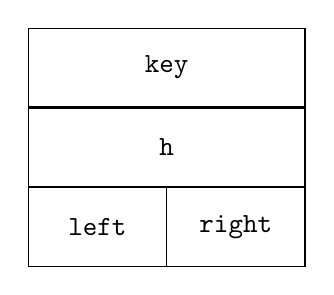
\begin{tikzpicture}[font=\ttfamily,minimum height=1cm]
\node (Key) [rectangle,draw,minimum width=10em] {\texttt{key}};
\node (Height) [rectangle,draw,anchor=north,minimum width=10em] at (Key.south) {\texttt{h}};
\node (LeftChild) [rectangle,draw,anchor=north west,minimum width=5em] at (Height.south west) {\texttt{left}};
\node (RightChild) [rectangle,draw,anchor=north east,minimum width=5em] at (Height.south east) {\texttt{right}};
\end{tikzpicture}
\caption{Nodo di un albero AVL}\label{fig:nodo_avl}
\end{figure}

\subsection{Inserimento in un albero AVL}
Consideriamo un generico albero \textsc{avl} $T$, che sappiamo essere anche binario di ricerca oltre che completo. Applicare l'algoritmo~\ref{lst:insert} per effettuare l'\textbf{inserimento di un nodo} all'interno di $T$ non è sufficiente di per sè per costruire un albero binario di ricerca che soddisfi la proprietà~\ref{avl_prop}. Sarà necessario quindi modificare l'algoritmo introducendo un'algoritmo che effettui un controllo sul bilanciamento e, nel caso si verifichi uno sbilanciamento dell'albero, lo rimetta ``a posto''.

\begin{lstlisting}[language=asd,caption={\textsc{Insert-AVL(T,k)}},label=lst:insert-avl]
if T @\neq@ NIL then
	if T@\rightarrow@ key < k then
		T@\rightarrow@ right = Insert-AVL(T@\rightarrow@ right, k)
		T = Bilancia-Destra(T)
	else if T@\rightarrow@ key > k then
		T@\rightarrow@ left = Insert-AVL(T@\rightarrow@ left, k)
		T = Bilancia-Sinistra(T)
	else
		T = Alloca-Nodo-AVL()
		T@\rightarrow@ key = k
		T@\rightarrow@ left = T@\rightarrow@ right = NIL
		T@\rightarrow@ h = 0
return T
\end{lstlisting}

Per non aggravare il costo computazionale dell'algoritmo \textsc{Insert} (Algoritmo~\ref{lst:insert-avl}) ci aspettiamo che le operazioni all'interno degli algoritmi di bilanciamento abbiano un costo costante $\Theta(1)$. Lo sbilanciamento in un albero \textsc{avl} può essere risolto con una \textbf{sequenza di operazioni di bilanciamento}, anche dette \textbf{rotazioni}, che staranno alla base degli algoritmi \textsc{Bilancia-Sinistra} (Algoritmo~\ref{lst:bilancia-sx}) e \textsc{Bilancia-Destra}.

\subsection{Le rotazioni}
Le rotazioni sono delle operazioni che permettono di ripristinare le proprietà di un albero bilanciato a fronte di operazioni che ne modificano la struttura. Queste sono di due tipi: \textbf{sinistra} e \textbf{destra}\footnote{Per destra e sinistra si intende il sottoalbero che scatena lo sbilanciamento in un nodo e non il senso della rotazione.}. Oltre alle rotazioni singole a sinistra e a destra, è possibile effettuare anche delle \textbf{rotazioni doppie} come la rotazione doppia a sinistra, ovvero una rotazione a sinistra seguita da una rotazione a destra\footnote{La rotazione doppia a destra è duale}.

\subsubsection{La rotazione sinistra}
Consideriamo l'albero mostrato in Figura~\ref{Avl_insert1.png}. Ciascun sottoalbero che si dirama dai nodi $x$ e $y$ hanno altezza $h$ in modo tale che il vertice $x$ non vede alcuno sbilanciamento, vale infatti:
\begin{displaymath}
||x\rightarrow left| - |x \rightarrow right|| = |(h+1) - h| = 1 \leq 1
\end{displaymath}
Effettuando un inserimento di un nodo nel sottoalbero $A$ si ottiene una violazione in radice della proprietà~\ref{avl_prop} (Figura~\ref{Avl_insert2.png}). Infatti, aggiungendo un nodo in $A$, si modifica la sua altezza che, da $h$, diventa $h+1$. Questo inserimento fa scendere l'albero radicato nel nodo $y$ ad una altezza $h+2$. Si ha così la violazione:
\begin{displaymath}
| |x \rightarrow left| - |x \rightarrow right||=|(h+2 )- h |=2 \nleq 1
\end{displaymath}

\begin{center}
\begin{minipage}{.45\textwidth}
\centering
\begin{tikzpicture}
\tikzset{
level 1/.style={sibling distance=2cm},
level 2/.style={sibling distance=1.5cm},
level 3/.style={sibling distance=0.5cm},
itria/.style={isosceles triangle,draw, dashed,shape border rotate=90,isosceles triangle stretches=true, minimum height=10mm,minimum width=12mm,inner sep=0,yshift={-20mm},fill=blue!25!white},
btria/.style={isosceles triangle,draw,dashed,shape border rotate=90,isosceles triangle stretches=true, minimum height=20mm,minimum width=12mm,inner sep=0,yshift={-20mm},fill=red!25!white},
mynode/.style={
  circle,
  draw,
  minimum size=0.5cm,
  fill=blue!25!white
}
}
\node[mynode,name=root]{x}
[child anchor=north]
child
{
  node[mynode,name=root_sx]{y}
    child
    {
     node[itria,name=A_tree]{A}
    }
    child
    {
      node[itria,name=B_tree]{B}
    }
}
child
{
  node[itria,name=C_tree]{C}
};
\node[anchor=east]at(root.west){$+1$};
\node[anchor=east]at(root_sx.west){$+0$};
\end{tikzpicture}
\captionof{figure}{Albero \textsc{AVL} bilanciato: accanto a ciascun vertice è presente la differenza, in valore assoluto, tra le altezze dei sottoalberi.\label{Avl_insert1.png}}
\end{minipage}
\hfil
\begin{minipage}{.45\textwidth}
\centering
\begin{tikzpicture}
\tikzset{
level 1/.style={sibling distance=3cm},
level 2/.style={sibling distance=1.5cm},
level 3/.style={sibling distance=0.75cm},
itria/.style={isosceles triangle,draw, dashed,shape border rotate=90,isosceles triangle stretches=true, minimum height=10mm,minimum width=12mm,inner sep=0,yshift={-20mm},fill=blue!25!white},
btria/.style={isosceles triangle,draw,dashed,shape border rotate=90,isosceles triangle stretches=true, minimum height=20mm,minimum width=12mm,inner sep=0,yshift={-20mm},fill=red!25!white},
mynode/.style={
  circle,
  draw,
  minimum size=0.5cm,
  fill=blue!25!white
}
}
\node[mynode,name=root]{x}
[child anchor=north]
child
{
  node[mynode,name=root_sx]{y}
    child
    {
      node[btria,name=A_tree]{A}
    }
    child
    {
      node[itria,name=B_tree]{B}
    }
}
child
{
 node[itria,name=root_dx]{C}
};
\node[anchor=east]at(root.west){$+2$};
\node[anchor=east]at(root_sx.west){$+1$};
\end{tikzpicture}
\captionof{figure}{Albero \textsc{AVL} sbilanciato: il nodo $x$ vede aumentata la sua altezza\label{Avl_insert2.png}}
\end{minipage}
\end{center}

Come è possibile sistemare la violazione in questa situazione? Essendo stato il sottoalbero sinistro $A$ ad aver generato la violazione nel nodo $x$ si adotterà un'operazione di \textbf{rotazione singola sinistra} che avrà l'effetto di ruotare il nodo $x$ con il suo nodo figlio sinistro, ovvero il nodo $y$. L'operazione è molto semplice e consta dei seguenti passaggi:
\begin{enumerate}
\item Il nodo $y$, ovvero il figlio sinistro del nodo in cui si riscontra la violazione della proprietà~\ref{avl_prop}, \textbf{sale in radice};
\item Il nodo $x$ diventa \textbf{figlio destro} del nodo $y$;
\item Nel momento in cui $y$ ha come figlio destro il nodo $x$ e come figlio sinistro il vecchio albero $A$, si sposta l'albero $B$ come \textbf{figlio sinistro} del nodo $x$. È corretto fare questo spostamento in quanto tutti i nodi di $B$ continuano a stare a destra del nodo $y$ e a sinistra del nodo $x$.
\end{enumerate}

\begin{center}
\begin{minipage}{.45\textwidth}
\centering
\begin{tikzpicture}
\tikzset{
level 1/.style={sibling distance=3cm},
level 2/.style={sibling distance=1.5cm},
level 3/.style={sibling distance=0.75cm},
itria/.style={isosceles triangle,draw, dashed,shape border rotate=90,isosceles triangle stretches=true, minimum height=10mm,minimum width=12mm,inner sep=0,yshift={-20mm},fill=blue!25!white},
btria/.style={isosceles triangle,draw,dashed,shape border rotate=90,isosceles triangle stretches=true, minimum height=20mm,minimum width=12mm,inner sep=0,yshift={-20mm},fill=red!25!white},
mynode/.style={
  circle,
  draw,
  minimum size=0.5cm,
  fill=blue!25!white
}
}
\node[mynode,name=root]{x}
[child anchor=north]
child
{
  node[mynode,name=root_sx]{y}
    child
    {
      node[btria,name=A_tree]{A}
    }
    child[dashed]
    {
      node[itria,name=B_tree]{B}
    }
}
child
{
  node[itria,name=C_tree]{C}
};
\draw[->,red,thick](root_sx.north)to[bend left=35](root.west);
\draw[-,dashed,red,opacity=.8](B_tree)--(root);
\node[anchor=west]at(root.east){$+2$};
\node[anchor=east]at(root_sx.west){$+1$};
\end{tikzpicture}
\captionof{figure}{Rotazione singola sinistra}
\end{minipage}
\hfil
\begin{minipage}{.45\textwidth}
\centering
\begin{tikzpicture}
\tikzset{
level 1/.style={sibling distance=2cm},
level 2/.style={sibling distance=1.5cm},
level 3/.style={sibling distance=0.75cm},
itria/.style={isosceles triangle,draw, dashed,shape border rotate=90,isosceles triangle stretches=true, minimum height=10mm,minimum width=12mm,inner sep=0,yshift={-10mm},fill=blue!25!white},
btria/.style={isosceles triangle,draw,dashed,shape border rotate=90,isosceles triangle stretches=true, minimum height=20mm,minimum width=12mm,inner sep=0,yshift={-20mm},fill=red!25!white},
mynode/.style={
  circle,
  draw,
  minimum size=0.5cm,
  fill=blue!25!white
}
}
\node[mynode,name=root]{y}
[child anchor =north]
child
{
  node[btria,name=A_tree]{A}
}
child{
  node[mynode,name=root_dx]{x}
    child{
      node[itria,name=B_tree]{B}
    }
    child{
    node[itria,name=C_tree]{C}
    }
};
\node[anchor=west]at(root.east){$+0$};
\node[anchor=west]at(root_dx.east){$+0$};
\end{tikzpicture}
\captionof{figure}{Albero risultante dopo la rotazione singola sinistra\label{RotazioneSS_avl.png}}
\end{minipage}
\end{center}

In questo modo l'albero $A$ è salito di un livello mentre l'albero $C$ è sceso di un livello. Si osserva inoltre che, a fronte di un inserimento (che determina una rotazione), \textbf{l'operazione di ribilanciamento ripristina l'altezza dell'albero}. Infatti prima e dopo la rotazione si avrà: \[T \rightarrow h = h+2\] Si ottiene così l'albero in Figura~\ref{RotazioneSS_avl.png} che è ancora un albero \textsc{avl}. Infatti:
\begin{displaymath}
| |x \rightarrow left| - |x \rightarrow right||=|(h+1) - (h+1) |= 0 \leq 1
\end{displaymath}

L'algoritmo \textsc{Rotazione-Sx}(Algoritmo~\ref{lst:rotazione-sx}) prende in ingresso l'indirizzo della testa dell'albero e deve lavorare su due nodi: la radice che viene data in ingresso e la radice del sottoalbero sinistro che genera lo sbilanciamento. È facile vedere che l'algoritmo~\ref{lst:rotazione-sx} è eseguibile a tempo costante.

\begin{lstlisting}[language=asd,caption={Rotazione-Sx(T)},label=lst:rotazione-sx]
newT = T@\rightarrow@left
T@\rightarrow@left = newT@\rightarrow@right
newT@\rightarrow@right = T
T@\rightarrow@h = max(Altezza(T@\rightarrow@left), Altezza(T@\rightarrow@right))+1
newT@\rightarrow@h = max(Altezza(newT@\rightarrow@left), Altezza(newT@\rightarrow@right))+1
return newT
\end{lstlisting}

L'operazione di rotazione singola sinistra non fa altro che sollevare di un livello il sottoalbero $A$ e far scendere $C$. Il sottoalbero $B$ resta allo stesso livello dopo l'operazione di rotazione. Quindi se l'inserimento venisse fatto in $B$ determinando un'incremento dell'altezza di $B$ (sbilanciando di conseguenza il nodo $x$), l'operazione di rotazione singola sinistra lascerebbe immutato lo sbilanciamento.

Per questo motivo sarà necessario utilizzare una doppia operazione di bilanciamento che consiste di una prima rotazione a destra per portarci nel caso di uno sbilanciamento a sinistra e successivamente ripristinare l'albero con una rotazione a sinistra.

\subsubsection{La rotazione destra}
La rotazione destra è duale alla rotazione sinistra. Si consideri l'albero \textsc{avl} mostrato in Figura~\ref{fig:avl-rotazionedx}. In questo caso l'inserimento di un nodo nel sottoalbero $B$ del figlio destro della radice genera una violazione della proprietà~\ref{avl_prop} come si vede in Figura~\ref{fig:avl-sbilanciatodx}. Infatti:
\begin{displaymath}
| |x \rightarrow left| - |x \rightarrow right||=|(h) - (h+2) |=2 \nleq 1
\end{displaymath}

\begin{center}
\begin{minipage}{.45\textwidth}
\centering
\begin{tikzpicture}
\tikzset{
    level 1/.style={sibling distance=2cm},
    level 2/.style={sibling distance=1.5cm},
    level 3/.style={sibling distance=0.5cm},
    itria/.style={isosceles triangle,draw, dashed,shape border rotate=90,isosceles triangle stretches=true, minimum height=10mm,minimum width=12mm,inner sep=0,yshift={-10mm},fill=blue!25!white},
    btria/.style={isosceles triangle,draw,dashed,shape border rotate=90,isosceles triangle stretches=true, minimum height=20mm,minimum width=12mm,inner sep=0,yshift={-20mm},fill=red!25!white},
     mynode/.style={
       	circle,
       	draw,
       	minimum size=0.5cm,
       	fill=blue!25!white
    }
  }
  \node[mynode, name=root]{x}
  [child anchor=north]
  child
  {
      node[itria, name=C_tree]{C}
  }
  child
  {
    node[mynode, name=root_dx]{y}
    child
    {
        node[itria, name=A_tree]{A}
    }
    child
    {
        node[itria, name=B_tree]{B}
    }
  };
\node[anchor=west]at(root.east){$+1$};
\node[anchor=west]at(root_dx.east){$+0$};
\end{tikzpicture}
\captionof{figure}{Albero \textsc{avl} ben bilanciato\label{fig:avl-rotazionedx}}
\end{minipage}
\hfil
\begin{minipage}{.45\textwidth}
\centering
\begin{tikzpicture}
  \tikzset{
    level 1/.style={sibling distance=2cm},
    level 2/.style={sibling distance=1.5cm},
    level 3/.style={sibling distance=0.5cm},
    itria/.style={isosceles triangle,draw, dashed,shape border rotate=90,isosceles triangle stretches=true, minimum height=10mm,minimum width=12mm,inner sep=0,yshift={-10mm},fill=blue!25!white},
    btria/.style={isosceles triangle,draw,dashed,shape border rotate=90,isosceles triangle stretches=true, minimum height=20mm,minimum width=12mm,inner sep=0,yshift={-20mm},fill=red!25!white},
    mynode/.style={
      circle,
      draw,
      minimum size=0.5cm,
      fill=blue!25!white
    }
  }
  \node[mynode, name=root]{x}
  [child anchor= north]
  child
  {
    node[itria, name=C_tree]{C}
  }
  child
  {
    node[mynode, name=root_dx]{y}
    child
    {
        node[itria, name=A_tree]{A}
    }
    child
    {
        node[btria, name=B_tree]{B}
    }
  };
\node[anchor=west]at(root.east){$+2$};
\node[anchor=west]at(root_dx.east){$+1$};
\end{tikzpicture}
\captionof{figure}{Albero \textsc{AVL} sbilanciato\label{fig:avl-sbilanciatodx}}
\end{minipage}
\end{center}

In questo caso si applica una rotazione singola destra che ha l'effetto di far scendere il sottoalbero $C$ e far salire il sottoalbero $B$. L'altezza del sottoalbero $A$ rimane invariata come mostrato in Figura\ref{fig:rotazionedx}.

\begin{center}
\begin{minipage}{.45\textwidth}
\centering
\begin{tikzpicture}
  \tikzset{
    level 1/.style={sibling distance=2cm},
    level 2/.style={sibling distance=1.5cm},
    level 3/.style={sibling distance=0.5cm},
    itria/.style={isosceles triangle,draw, dashed,shape border rotate=90,isosceles triangle stretches=true, minimum height=10mm,minimum width=12mm,inner sep=0,yshift={-10mm},fill=blue!25!white},
    btria/.style={isosceles triangle,draw,dashed,shape border rotate=90,isosceles triangle stretches=true, minimum height=20mm,minimum width=12mm,inner sep=0,yshift={-20mm},fill=red!25!white},
    mynode/.style={ circle,draw, minimum size=0.5cm,fill=blue!25!white}
  }
  \node[mynode, name=root]{x}
  [child anchor = north]
  child
  {
    node[itria, name=C_tree]{C}
  }
  child
  {
    node[mynode, name=root_dx]{y}
    child [dashed]
    {
        node[itria, name=A_tree]{A}
    }
    child
    {
        node[btria, name=B_tree]{B}
    }
};
 \draw[->,red,thick](root_dx)to[bend right=35](root.east);
   \node[anchor=east]at(root.west){$+2$};
 \node[anchor=west]at(root_dx.east){$+1$};
 \draw[dashed,red](A_tree)--(root);
\end{tikzpicture}
\captionof{figure}{Rotazione singola destra\label{fig:rotazionedx}}
\end{minipage}
\hfil
\begin{minipage}{.45\textwidth}
\centering
\begin{tikzpicture}
\tikzset{
    level 1/.style={sibling distance=2cm},
    level 2/.style={sibling distance=1.5cm},
    level 3/.style={sibling distance=0.5cm},
    itria/.style={isosceles triangle,draw, dashed,shape border rotate=90,isosceles triangle stretches=true, minimum height=10mm,minimum width=12mm,inner sep=0,yshift={-10mm},fill=blue!25!white},
    btria/.style={isosceles triangle,draw,dashed,shape border rotate=90,isosceles triangle stretches=true, minimum height=20mm,minimum width=12mm,inner sep=0,yshift={-20mm},fill=red!25!white},
    mynode/.style={
      circle,
      draw,
      minimum size=0.5cm,
      fill=blue!25!white
    },
  }
  \node[mynode, name=root]{y}
  [child anchor = north]
  child
  {
      	node[mynode, name=root_sx]{x}
       child
       {
          	node[itria, name=C_tree]{C}
       }
       child
       {
          	node[itria, name=A_tree]{A}
       }
}
child
{
      	node[btria, name=B_tree]{B}
  };
\node[anchor=east]at(root.west){$+1$};
\node[anchor=west]at(root_sx.east){$+0$};
\end{tikzpicture}
\captionof{figure}{Albero risultante dopo la rotazione singola destra\label{fig:rotazionedx2}}
\end{minipage}
\end{center}

L'algoritmo \textsc{Rotazione-Dx} (Algoritmo~\ref{lst:rotazione-dx}) è duale all'algoritmo \textsc{Rotazione-Sx} (Algoritmo~\ref{lst:rotazione-sx}).

\begin{lstlisting}[language=asd,caption={Rotazione-Dx(T)},label=lst:rotazione-dx]
newT = T@\rightarrow@right
T@\rightarrow@right = newT@\rightarrow@left
newT@\rightarrow@left = T
T@\rightarrow@h = max(Altezza(T@\rightarrow@left), Altezza(T@\rightarrow@right))+1
newT@\rightarrow@h = max(Altezza(newT@\rightarrow@left), Altezza(newT@\rightarrow@right))+1
return newT
\end{lstlisting}
\subsubsection{La doppia rotazione sinistra}
Si consideri l'albero $T$ come mostrato in Figura~\ref{fig:albero-avl-case2}. I sottoalberi $A$ e $D$ hanno altezza $h-2$ mentre i sottoalberi $B$ e $C$ hanno altezza $h-3$. L'albero radicato in $x$ risulta così ben bilanciato, infatti vale:
\begin{displaymath}
||x \rightarrow left| - |x \rightarrow right|| = |(h+1)-(h)| = +1 \leq 1
\end{displaymath}

\begin{center}
\begin{minipage}{.45\textwidth}
\centering
\begin{tikzpicture}
  \tikzset{
    level 1/.style={sibling distance=3cm},
    level 2/.style={sibling distance=2cm},
    level 3/.style={sibling distance=1.5cm},
    itria/.style={isosceles triangle,draw, dashed,shape border rotate=90,isosceles triangle stretches=true, minimum height=10mm,minimum width=12mm,inner sep=0,yshift={-10mm},fill=blue!25!white},
     btria/.style={isosceles triangle,draw,dashed,shape border rotate=90,isosceles triangle stretches=true, minimum height=20mm,minimum width=12mm,inner sep=0,yshift={-20mm},fill=red!25!white},
    ctria/.style={isosceles triangle,draw, dashed,shape border rotate=90,isosceles triangle stretches=true, minimum height=20mm,minimum width=12mm,inner sep=0,yshift={-20mm},fill=blue!25!white},
    mynode/.style={
       	circle,
       	draw,
       	minimum size=0.5cm,
       	fill=blue!25!white
    },
  }
  \node[mynode, name=root]{x}
  [child anchor = north]
  child
  {
    node[mynode,name=root_sx]{y}
    child
    {
      node[ctria, name=A_tree]{A}
    }
    child
    {
      node[mynode,name=y_dx]{z}
      child
      {
        node[itria, name=B_tree]{B}
      }
      child
      {
        node[itria, name=C_tree]{C}
      }
    }
  }
  child
  {
  node[ctria, name=D_tree]{D}
  };
\node[anchor=west]at(y_dx.east){$+0$};
\node[anchor=west]at(root_sx.east){$+0$};
\node[anchor=west]at(root.east){$+1$};
\end{tikzpicture}
\captionof{figure}{Albero \textsc{avl} ben bilanciato\label{fig:albero-avl-case2}}
\end{minipage}
\hfil
\begin{minipage}{.45\textwidth}
\centering
\begin{tikzpicture}
\tikzset{
    level 1/.style={sibling distance=3cm},
    level 2/.style={sibling distance=2cm},
    level 3/.style={sibling distance=1.5cm},
    itria/.style={isosceles triangle,draw, dashed,shape border rotate=90,isosceles triangle stretches=true, minimum height=10mm,minimum width=12mm,inner sep=0,yshift={-10mm},fill=blue!25!white},
     btria/.style={isosceles triangle,draw,dashed,shape border rotate=90,isosceles triangle stretches=true, minimum height=20mm,minimum width=12mm,inner sep=0,yshift={-20mm},fill=red!25!white},
    ctria/.style={isosceles triangle,draw, dashed,shape border rotate=90,isosceles triangle stretches=true, minimum height=20mm,minimum width=12mm,inner sep=0,yshift={-20mm},fill=blue!25!white},
    mynode/.style={
       	circle,
       	draw,
       	minimum size=0.5cm,
       	fill=blue!25!white
    },
  }
  \node[mynode, name=root]{x}
  [child anchor = north]
  child {
    node[mynode,name=root_sx]{y}
    child{
      node[ctria, name=A_tree]{A}
    }
    child{
      node[mynode,name=y_dx]{z}
      child
      {
        node[btria, name=B_tree]{B}
      }
      child
      {
        node[itria, name=C_tree]{C}
      }
    }
  }
  child {
    node[ctria, name=D_tree]{D}
  };
\node[anchor=west]at(y_dx.east){$+1$};
\node[anchor=west]at(root_sx.east){$+1$};
\node[anchor=west,red]at(root.east){$+2$};
\end{tikzpicture}
\captionof{figure}{Inserimento nel sottoalbero $B$\label{fig:sbilanciamento-case2}}
\end{minipage}
\end{center}

Supponiamo di inserire un nodo nel sottoalbero $B$ radicato in $z$. Ovviamente, a seguito dell'inserimento l'altezza di tale sottoalbero risulterà incrementata causando uno sbilanciamento sul nodo $x$ dato dal suo sottoalbero sinistro come mostrato in Figura \ref{fig:sbilanciamento-case2}:
\begin{displaymath}
||x \rightarrow left| - |x \rightarrow right|| = |(h)-(h-2)| = +2 \nleq 1
\end{displaymath}
L'idea alla base della \textbf{doppia rotazione} è quella di \textit{spostare il peso aggiuntivo} che si trova nel sottoalbero destro del nodo $y$ verso il suo sottoalbero sinistro in modo tale da ricondurci al caso di uno sbilanciamento a sinistra, risolvibile con una rotazione sinistra semplice. È necessario quindi effettuare una prima rotazione semplice destra che sposti tale peso verso il sottoalbero sinistro (vedi Figura~\ref{fig:rotazione-ds1}) e successivamente una rotazione semplice sinistra che risolva il problema (Figura~\ref{fig:rotazione-ds3}).

\begin{center}
\begin{minipage}{.45\textwidth}
\centering
\begin{tikzpicture}
  \tikzset{
    level 1/.style={sibling distance=3cm},
    level 2/.style={sibling distance=2cm},
    level 3/.style={sibling distance=1.5cm},
    itria/.style={isosceles triangle,draw, dashed,shape border rotate=90,isosceles triangle stretches=true, minimum height=10mm,minimum width=12mm,inner sep=0,yshift={-10mm},fill=blue!25!white},
    btria/.style={isosceles triangle,draw,dashed,shape border rotate=90,isosceles triangle stretches=true, minimum height=20mm,minimum width=12mm,inner sep=0,yshift={-20mm},fill=red!25!white},
    ctria/.style={isosceles triangle,draw, dashed,shape border rotate=90,isosceles triangle stretches=true, minimum height=20mm,minimum width=12mm,inner sep=0,yshift={-20mm},fill=blue!25!white},
    mynode/.style={
      circle,
      draw,
      minimum size=0.5cm,
      fill=blue!25!white
    }
  }
  \node[mynode, name=root]{x}
  [child anchor = north]
  child {
    node[mynode,name=root_sx]{y}
    child{
      node[ctria, name=A_tree]{A}
    }
    child{
      node[mynode,name=y_dx]{z}
      child[dashed]
      {
      node[btria, name=B_tree]{B}
      }
      child
      {
        node[itria, name=C_tree]{C}
      }
    }
  }
  child {
    node[ctria, name=D_tree]{D}
  };
\node[anchor=west]at(y_dx.east){$+1$};
\node[anchor=west]at(root_sx.east){$+1$};
\node[anchor=west,red]at(root.east){$+2$};
\draw[->,red,thick](y_dx.north)to[bend right=30](root_sx.east);
\draw[-,red,dashed](B_tree)--(root_sx);
\end{tikzpicture}
\captionof{figure}{Prima rotazione semplice destra\label{fig:rotazione-ds1}}
\end{minipage}
\hfil
\begin{minipage}{.45\textwidth}
\centering
\begin{tikzpicture}
  \tikzset{
    level 1/.style={sibling distance=3cm},
    level 2/.style={sibling distance=2cm},
    level 3/.style={sibling distance=1.5cm},
    itria/.style={isosceles triangle,draw, dashed,shape border rotate=90,isosceles triangle stretches=true, minimum height=10mm,minimum width=12mm,inner sep=0,yshift={-10mm},fill=blue!25!white},
    btria/.style={isosceles triangle,draw,dashed,shape border rotate=90,isosceles triangle stretches=true, minimum height=20mm,minimum width=12mm,inner sep=0,yshift={-20mm},fill=red!25!white},
    ctria/.style={isosceles triangle,draw, dashed,shape border rotate=90,isosceles triangle stretches=true, minimum height=20mm,minimum width=12mm,inner sep=0,yshift={-20mm},fill=blue!25!white},
    mynode/.style={
      circle,
      draw,
      minimum size=0.5cm,
      fill=blue!25!white
    }
  }
  \node[mynode, name=root]{x}
  [child anchor = north]
  child
  {
    node[mynode,name=root_sx]{z}
    child
    {
      node[mynode,name=y]{y}
      child
      {
        node[ctria, name=A_tree]{A}
      }
      child
      {
        node[btria, name=B_tree]{B}
      }
    }
    child
    {
      node[itria, name=C_tree]{C}
    }
  }
  child
  {
    node[ctria, name=D_tree]{D}
  };
\node[anchor=west]at(y.east){$+0$};
\node[anchor=west,red]at(root_sx.east){$+2$};
\node[anchor=west,red]at(root.east){$+2$};
\end{tikzpicture}
\captionof{figure}{Situazione a seguito della rotazione singola destra\label{fig:rotazione-ds2}}
\end{minipage}
\\
\begin{minipage}{.45\textwidth}
 	\centering
\begin{tikzpicture}
  \tikzset{
    level 1/.style={sibling distance=3cm},
    level 2/.style={sibling distance=2cm},
    level 3/.style={sibling distance=1.5cm},
    itria/.style={isosceles triangle,draw, dashed,shape border rotate=90,isosceles triangle stretches=true, minimum height=10mm,minimum width=12mm,inner sep=0,yshift={-10mm},fill=blue!25!white},
     btria/.style={isosceles triangle,draw,dashed,shape border rotate=90,isosceles triangle stretches=true, minimum height=20mm,minimum width=12mm,inner sep=0,yshift={-20mm},fill=red!25!white},
    ctria/.style={isosceles triangle,draw, dashed,shape border rotate=90,isosceles triangle stretches=true, minimum height=20mm,minimum width=12mm,inner sep=0,yshift={-20mm},fill=blue!25!white},
    mynode/.style={
      circle,
      draw,
      minimum size=0.5cm,
      fill=blue!25!white
    }
  }
  \node[mynode, name=root]{x}
  [child anchor = north]
  child {
    node[mynode,name=root_sx]{z}
    child{
      node[mynode,name=y]{y}
      child{
        node[ctria, name=A_tree]{A}
      }
      child{
        node[btria, name=B_tree]{B}
      }
    }
    child[dashed]{
      node[itria, name=C_tree]{C}
    }
  }
  child {
    node[ctria, name=D_tree]{D}
  };
  \node[anchor=west]at(y.east){$+0$};
\node[anchor=west,red]at(root_sx.east){$+2$};
\node[anchor=west,red]at(root.east){$+2$};
\draw[->,red,thick](root_sx.north)to[bend left=35](root);
\draw[-,dashed,red](C_tree.north)--(root.south);
\end{tikzpicture}
\captionof{figure}{Rotazione singola sinistra\label{fig:rotazione-ds3}}
\end{minipage}
\hfil
\begin{minipage}{.45\textwidth}
 	\centering
  \begin{tikzpicture}
  \tikzset{
    level 1/.style={sibling distance=3.5cm},
    level 2/.style={sibling distance=2.5cm},
    level 3/.style={sibling distance=1.5cm},
    itria/.style={isosceles triangle,draw, dashed,shape border rotate=90,isosceles triangle stretches=true, minimum height=10mm,minimum width=12mm,inner sep=0,yshift={-10mm},fill=blue!25!white},
    btria/.style={isosceles triangle,draw,dashed,shape border rotate=90,isosceles triangle stretches=true, minimum height=20mm,minimum width=12mm,inner sep=0,yshift={-20mm},fill=red!25!white},
    ctria/.style={isosceles triangle,draw, dashed,shape border rotate=90,isosceles triangle stretches=true, minimum height=20mm,minimum width=12mm,inner sep=0,yshift={-20mm},fill=blue!25!white},
    mynode/.style={
      circle,
      draw,
      minimum size=0.5cm,
      fill=blue!25!white
    }
  }
  \node[mynode, name=root]{z}
  [child anchor = north]
  child
  {
    node[mynode,name=root_sx]{y}
    child
    {
        node[ctria, name=A_tree]{A}
      }
      child
      {
        node[btria, name=B_tree]{B}
      }
    }
  child
  {
      node[mynode,name=root_dx]{x}
      child
      {
        node[itria, name=C_tree]{C}
      }
      child
      {
        node[ctria, name=D_tree]{D}
    }
  };
\node[anchor=west]at(root.east){$+0$};
\node[anchor=west]at(root_sx.east){$+0$};
\node[anchor=west]at(root_dx.east){$+1$};
\end{tikzpicture}
\captionof{figure}{Albero risultante\label{fig:rotazione-ds4}}
\end{minipage}
\end{center}

Si ottiene così l'albero in Figura~\ref{fig:rotazione-ds4} che è ancora un albero \textsc{avl}. Infatti:
\begin{displaymath}
| |x \rightarrow left| - |x \rightarrow right||=|(h-1) - (h-1) |=1 \leq 1
\end{displaymath}

\begin{lstlisting}[language=asd,caption={\textsc{Rotazione-Doppia-Sx}},label=lst:rotazione-doppia-sx]
T@\rightarrow@left = Rotazione-Destra(T@\rightarrow@left)
T = Rotazione-Sinistra(T)
return T
\end{lstlisting}

Date queste operazioni di rotazione possiamo scrivere dunque l'algoritmo \textsc{Bilancia-Sx}$(T)$ (Algoritmo~\ref{lst:bilancia-sx}). L'algoritmo \textsc{Bilancia-Dx} sarà duale.

\begin{lstlisting}[label=lst:bilancia-sx,caption={Bilancia-Sx(T)},language=asd]
if T@\neq@ NIL then
if Altezza(T @\rightarrow@ left) - Altezza(T@\rightarrow@ right) > 1 then
  Sx = T@\rightarrow@ left
  if Altezza(Sx @\rightarrow@ left) >= Altezza(Sx @\rightarrow@ right) then
    T = Rotazione-Sinistra(T)
  else
    T = Rotazione-Doppia-Sinistra(T)
else
  T@\rightarrow@ h = max(Altezza(T@\rightarrow@ left), Altezza(T@\rightarrow@ right))+1
return T
\end{lstlisting}


\begin{osservation}
A fronte di un inserimento in un albero \textsc{avl} possiamo osservare che \textbf{possono avvenire al più due rotazioni}. Infatti, se un inserimento causa uno sbilanciamento, questo può essere risolto con una rotazione semplice o con una rotazione doppia. In entrambi i casi, l'altezza dell'albero viene incrementata di al più un livello. Se un inserimento non causa uno sbilanciamento, ciò significa che l'altezza dell'albero non è stata incrementata e non sarà necessaria alcuna rotazione.
\end{osservation}


\subsection{Cancellazione in un albero AVL}
Come per l'inserimento di un nodo all'interno di un albero \textsc{avl}, anche l'operazione di cancellazione richiede un'operazione di \textit{ribilanciamento} dell'albero in quanto, facendo diminuire l'altezza di un sottoalbero, non è garantito che sul padre, la differenza in altezza con il sottoalbero fratello rispetti la proprietà~\ref{avl_prop}.

Analogamente a quanto visto nel caso della cancellazione in un albero binario di ricerca, anche per gli alberi AVL si discriminano tre casi: cancellazione di un nodo foglia, cancellazione di un nodo con un solo figlio e cancellazione di un nodo con due figli.  In questo caso, però, non è detto che una singola operazione di ribilanciamento sia sufficiente a riportare l'albero in uno stato di bilanciamento. Infatti, la cancellazione di un nodo può causare uno sbilanciamento in un nodo diverso da quello cancellato. Per questo motivo, l'operazione di cancellazione prevede un'operazione di ribilanciamento dell'albero che potrebbe essere eseguita in modo ricorsivo fino a che non si raggiunge la radice dell'albero. Dovremo quindi effettuare delle modifiche degli algoritmi visti per la cancellazione in un albero binario di ricerca.

\begin{center}
\begin{minipage}{.45\textwidth}
\begin{lstlisting}[language=asd,caption={\textsc{Delete}(T,k)},label=lst:delete-avl]
if T @\neq@ NIL then
if T @\rightarrow@ key > k then
T @\rightarrow@ left = Delete(T @\rightarrow@ left, k)
T = Bilancia-Destra(T)
else if T @\rightarrow@ key < k then
T @\rightarrow@ right = Delete(T @\rightarrow@ right, k)
T = Bilancia-Sx(T)
else
T = Delete-Root(T)
return T
\end{lstlisting}
\end{minipage}
\hfil
\begin{minipage}{.45\textwidth}
\begin{lstlisting}[language=asd,caption={\textsc{Delete-Root}(T)},label=lst:delete-root-avl]
if T @\neq@ NIL then
tmp = T
if T@\rightarrow@ left = NIL then
T = T@\rightarrow@ right
else if T@\rightarrow@ right = NIL then
T = T@\rightarrow@ left
else
tmp = Stacca-Min(T@\rightarrow@ right)
T@\rightarrow@ key = tmp @\rightarrow@ key
T = Bilancia-Sx(T)
free(tmp)
return T
\end{lstlisting}
\end{minipage}
\end{center}

\begin{lstlisting}[language=asd,caption={Stacca-MinAVL(T,P)},label=lst:stacca-min-avl]
if T@\neq@ NIL && P@\neq@ NIL then
if T @\rightarrow@ left @\neq@ NIL then
ret = Stacca-MinAVL(T @\rightarrow@ left, T)
newT = Bilancia-Dx(T)
else
ret = T
newT = T @\rightarrow@ right
if T = P @\rightarrow@ left then
P @\rightarrow@ left = newT
else
P @\rightarrow@ right = newT
return ret
\end{lstlisting}

Osserviamo un particolare caso di cancellazione: la cancellazione della foglia di minor altezza. Consideriamo l'albero AVL di altezza cinque mostrato in Figura~\ref{fig:delete-avl-leaf}. Supponiamo di voler cancellare la foglia più a destra ad altezza $2$. La cancellazione di tale nodo causa uno sbilanciamento che si propaga fino alla radice. Si dimostra per induzione, che in un albero AVL, la foglia con altezza minore si trova sempre a metà altezza dell'albero. Ne segue che il numero di rotazioni necessarie per ri-bilanciare l'albero è lineare sull'altezza dell'albero, ovvero logaritmico sul numero dei nodi.

\begin{figure}[ht!]
\centering
\begin{forest}
important/.style={name=#1,fill=red!20!white},
for tree={
      circle,
      draw,
      minimum size=0.5cm,
      fill=blue!25!white,
    }
    [
      [
    [
    [
      [
        []
        [,phantom]
      ]
      []
    ]
    [
    []
    [,phantom]
  ]
  ]
  [
    [
      []
      [,phantom]
    ]
    []
  ]
  ]
  [
    [
      [
        []
        [,phantom]
      ]
      []
    ]
    [
    [,important] % nodo da cancellare
    [,phantom]
  ]
  ]
    ]
\end{forest}
\caption{Cancellazione di un nodo foglia in un albero AVL di altezza cinque}\label{fig:delete-avl-leaf}
\end{figure}


\section{Alberi rossi e neri}
Nelle sezioni precedenti si è visto che un albero binario di ricerca di altezza $h$ può implementare qualsiasi operazione sugli insiemi dinamici in un tempo lineare sull'altezza dell'albero. Queste operazioni sono, quindi, veloci  se l'altezza dell'albero resta contenuta. A fronte di una sequenza di operazioni di inserimento e cancellazione, l'altezza dell'albero può variare notevolmente inficiando le prestazioni delle operazioni stesse. Per questo motivo, si è cercato di definire una struttura dati che garantisca un'altezza contenuta dell'albero binario di ricerca. Così come gli alberi AVL, anche gli alberi rossi e neri rappresentano uno dei tanti modi\footnote{Splay Trees, B Alberi, ecc.} in cui gli alberi binari di ricerca vengono ``bilanciati'' per garantire che le operazioni elementari sugli insiemi dinamici richiedano un tempo logaritmico sul numero dei nodi.

\subsection{Proprietà degli alberi rosso-neri}
Un \textbf{albero rosso-nero} è un albero binario di ricerca con un campo aggiuntivo di memoria per ogni nodo: il \textbf{colore} del nodo, che può essere \textsc{RED} o \textsc{BLACK}. Assegnando dei vincoli al modo in cui i nodi possono essere colorati, si garantisce che l'altezza dell'albero sia logaritmica sul numero dei nodi.

Ciascun nodo dell'albero contiene i campi: \textit{color, key, left, right, h} (Figura~\ref{fig:rb-node}). Il colore di ciascun nodo può essere espresso mediante una funzione di tipo booleana che ad ogni nodo assegna un bit a 0 o 1 a seconda che il colore sia rosso o nero. In questo modo, il colore di un nodo può essere rappresentato con un singolo bit di memoria a differenza del campo altezza che è rappresentato da un valore intero.

\begin{figure}[ht!]
\centering
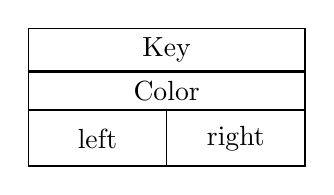
\begin{tikzpicture}
  \node (Key) [rectangle,draw,minimum width=10em] {Key};
  \node (Color) [rectangle,draw,anchor=north,minimum width=10em] at (Key.south) {Color};
  \node (LeftChild) [rectangle,draw,anchor=north west,minimum width=5em,,minimum height=0.7cm] at ( Color.south west) {left};
  \node (RightChild) [rectangle,draw,anchor=north east,minimum width=5em,,minimum height=0.7cm] at (Color.south east) {right};
\end{tikzpicture}
\caption{Implementazione di un nodo di un albero R\&B}\label{fig:rb-node}
\end{figure}

\dfn{Alberi R-B}{
Un albero rosso e nero è un albero binario di ricerca che rispetta i seguenti vincoli:
\begin{enumerate}
\item Ogni nodo è colorato di rosso o di nero;
\item Ogni foglia è colorata di nero e non contiene dati. Queste foglie sono dette \textbf{foglie esterne} o \textbf{NIL};
\item La radice è nera;
\item Ogni nodo rosso ha solo figli neri;
\item Per ogni nodo $x$, ogni percorso da $x$ a un nodo NIL contiene lo stesso numero di nodi neri. Questa quantità è detta \textbf{altezza nera} di $x$ e viene indicata con $bh(x)$.
\end{enumerate}
}

La Figura~\ref{fig:rb-tree} mostra un esempio di albero rosso-nero. In questo caso, il numero di nodi neri lungo ogni percorso da un nodo a una foglia esterna è sempre 3. È facile osservare che tutti gli alberi AVL possono essere alberi rossi e neri, secondo un'opportuna colorazione, ma non tutti gli alberi rossi e neri possono essere degli alberi AVL. Si consideri l'albero mostrato in Figura~\ref{fig:rb-not-avl}. Questo albero è un albero rosso nero in quanto rispetta ogni proprietà, ma non è un albero AVL in quanto la differenza di altezza tra il sottoalbero sinistro e quello destro del nodo $x$ è maggiore di 1. In Figura~\ref{fig:gerarchia-alberi} è mostrata la gerarchia degli alberi binari di ricerca perfettamente bilanciati, AVL e rossi e neri.

\begin{figure}[ht!]
\centering
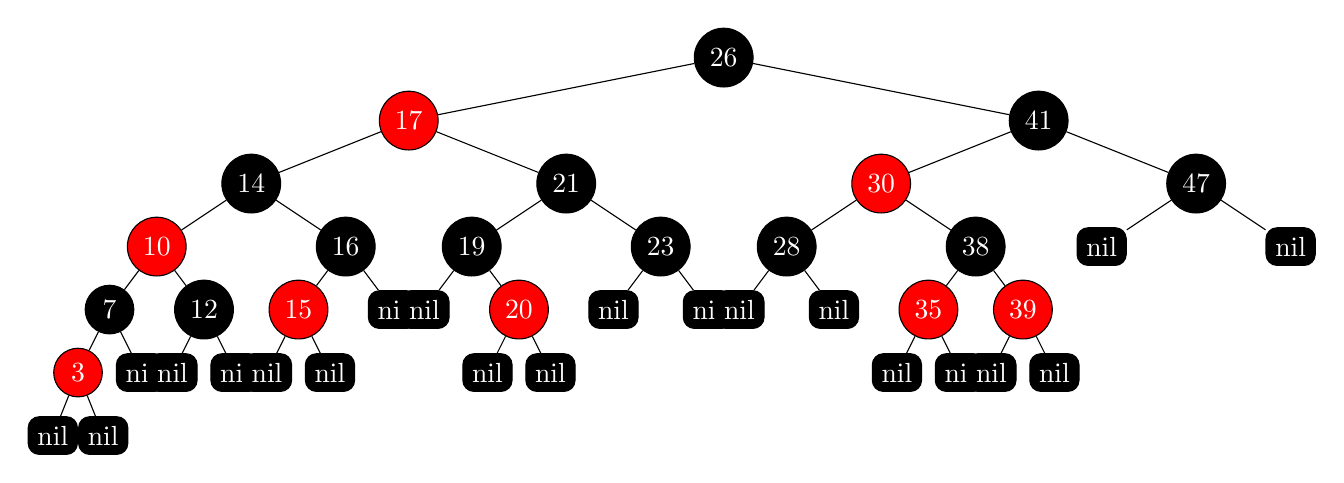
\begin{tikzpicture}
[level 1/.style={level distance=1cm, sibling distance=10cm},
level 2/.style={sibling distance=5cm},
level 3/.style={sibling distance=3cm},
level 4/.style={sibling distance=1.5cm},
level 5/.style={sibling distance=1cm},
level 6/.style={sibling distance=0.8cm},
root/.style={circle,draw,fill=black,text=white,minimum size=0.5cm},
rednode/.style={circle,draw,fill=red,text=white,minimum size=0.5cm},
blacknode/.style={circle,draw,fill=black,text=white,minimum size=0.5cm},
leaf/.style={rectangle,rounded corners,draw,fill=black,text=white,minimum height = 2mm, minimum width = 2mm},scale=0.8]
\node[root]{26}
child {
  node[rednode]{17}
    child{
      node[blacknode]{14}
      child{
        node[rednode]{10}
        child{
          node[blacknode]{7}
          child{
            node[rednode]{3}
            child{
              node[leaf]{nil}
            }
            child{
              node[leaf]{nil}
            }
          }
          child{
            node[leaf]{nil}
          }
        }
        child{
          node[blacknode]{12}
          child{
            node[leaf]{nil}
          }
          child{
            node[leaf]{nil}
          }
        }
      }
      child{
        node[blacknode]{16}
        child{
          node[rednode]{15}
          child{
            node[leaf]{nil}
          }
          child{
            node[leaf]{nil}
          }
        }
        child{
          node[leaf]{nil}
        }
      }
    }
    child{
      node[blacknode]{21}
      child{
        node[blacknode]{19}
        child{
          node[leaf]{nil}
        }
        child{
          node[rednode]{20}
          child{
            node[leaf]{nil}
          }
          child{
            node[leaf]{nil}
          }
        }
      }
      child{
        node[blacknode]{23}
        child{
          node[leaf]{nil}
        }
        child{
          node[leaf]{nil}
        }
      }
    }
}
child{
  node[blacknode]{41}
  child{
    node[rednode]{30}
    child{
      node[blacknode]{28}
      child{
        node[leaf]{nil}
      }
      child{
        node[leaf]{nil}
      }
    }
    child{
      node[blacknode]{38}
      child{
        node[rednode]{35}
        child{
          node[leaf]{nil}
        }
        child{
          node[leaf]{nil}
        }
      }
      child{
        node[rednode]{39}
        child{
          node[leaf]{nil}
        }
        child{
          node[leaf]{nil}
        }
      }
    }
  }
  child{
    node[blacknode]{47}
    child{
      node[leaf]{nil}
    }
    child{
      node[leaf]{nil}
    }
  }
};
\end{tikzpicture}
\caption{Albero rosso e nero}\label{fig:rb-tree}
\end{figure}

\begin{figure}[ht!]
\centering
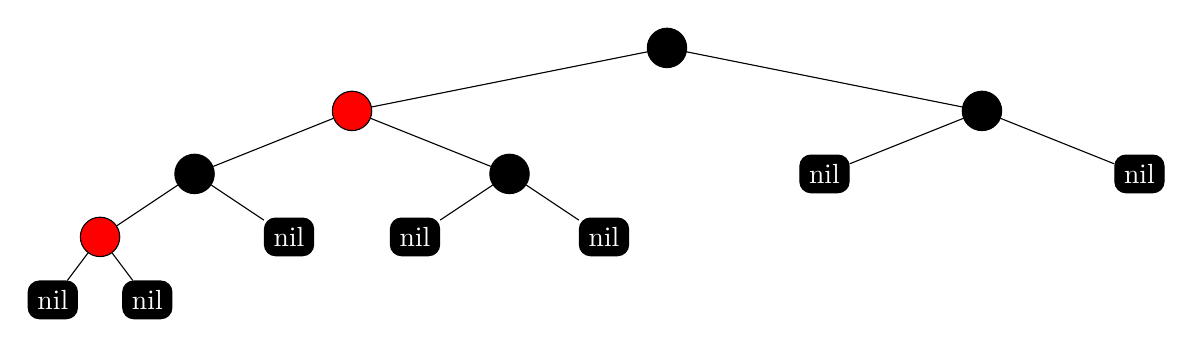
\begin{tikzpicture}
[level 1/.style={level distance=1cm, sibling distance=10cm},
level 2/.style={sibling distance=5cm},
level 3/.style={sibling distance=3cm},
level 4/.style={sibling distance=1.5cm},
level 5/.style={sibling distance=1cm},
level 6/.style={sibling distance=0.8cm},
root/.style={circle,draw,fill=black,text=white,minimum size=0.5cm},
rednode/.style={circle,draw,fill=red,text=white,minimum size=0.5cm},
blacknode/.style={circle,draw,fill=black,text=white,minimum size=0.5cm},
leaf/.style={rectangle,rounded corners,draw,fill=black,text=white,minimum height = 2mm, minimum width = 2mm},scale=.8]
\node[root]{}
child{
  node[rednode]{}
  child{
    node[blacknode]{}
    child{
      node[rednode]{}
      child{
        node[leaf]{nil}
      }
      child{
        node[leaf]{nil}
      }
    }
    child{
      node[leaf]{nil}
    }
  }
  child{
    node[blacknode]{}
    child{
      node[leaf]{nil}
    }
    child{
      node[leaf]{nil}
    }
  }
}
child{
  node[blacknode]{}
  child{
    node[leaf]{nil}
  }
  child{
    node[leaf]{nil}
  }
};
\end{tikzpicture}
\caption{Albero rosso e nero che non è un albero AVL}\label{fig:rb-not-avl}
\end{figure}


\begin{osservation}
Come si evince dal diagramma mostrato in Figura~\ref{fig:gerarchia-alberi} un albero pieno può essere colorabile come un albero rosso e nero. Un modo per colorarlo, infatti, è fare tutti i suoi nodi di nero. Questo perché gli alberi pieni hanno tutti i livelli saturi e di conseguenza tutti i percorsi da qualche nodo a una foglia avranno la stessa lunghezza. Un altro modo per colorarlo è alternando un livello rosso con un livello nero. Questo perché, essendo l'albero pieno, tutti i nodi di un livello hanno lo stesso numero di figli e, quindi, tutti i percorsi da qualche nodo a una foglia avranno la stessa lunghezza.
\end{osservation}


Non tutti gli alberi, però, sono colorabili. Sia ad esempio $T$ un albero binario come mostrato in Figura~\ref{fig:tree-not-colorable}. Da come si vede da questo esempio, nonostante i vincoli definiti per gli alberi rosso neri siano meno restrittivi di quanto visto per gli alberi AVL e APB, non tutti gli alberi binari di ricerca possono essere colorati come alberi rossi e neri. In particolare, un altro esempio di albero non colorabile è dato dalla classe degli alberi degeneri.

\begin{figure}[ht!]
\centering
\subfloat[\label{fig:tree-not-colorable}]{
	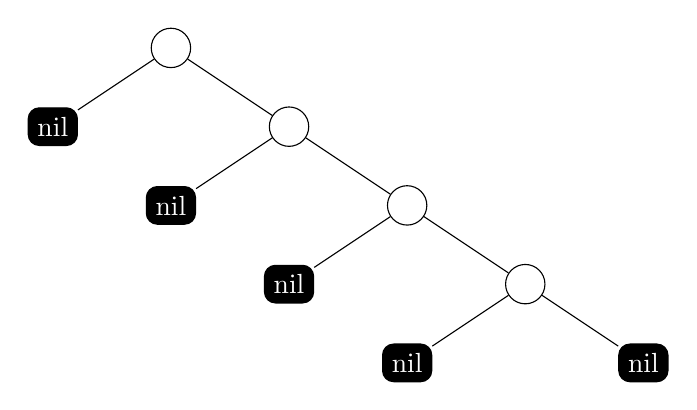
\begin{tikzpicture}
		[
		level 1/.style={level distance=1cm, sibling distance=3cm},
		level 2/.style={sibling distance=3cm},
		level 3/.style={sibling distance=3cm},
		level 4/.style={sibling distance=3cm},
		level 5/.style={sibling distance=3cm},
		level 6/.style={sibling distance=3cm},
		mynode/.style={
			circle,
			draw,
			minimum size=0.5cm
		},
		leaf/.style={rectangle,rounded corners,draw,fill=black,text=white,minimum height = 2mm, minimum width = 2mm}]
		\node[mynode]{}
		child{
			node[leaf]{nil}
		}
		child
		{
			node[mynode]{}
			child{
				node[leaf]{nil}
			}
			child{
				node[mynode]{}
				child{
					node[leaf]{nil}
				}
				child{
					node[mynode]{}
					child{
						node[leaf]{nil}
					}
					child{
						node[leaf]{nil}
					}
				}
			}
		};
\end{tikzpicture}} \qquad
\subfloat[Il colore della radice è ininfluente. Se è rossa, allora per il vincolo 3 il figlio dovrà essere nero. Così facendo notiamo però che il vincolo 4 non è rispettato. Il percorso che dalla radice arriva alla foglia ha un solo nodo nero, mentre il percorso che arriva alla foglia successiva ne ha due.]{
	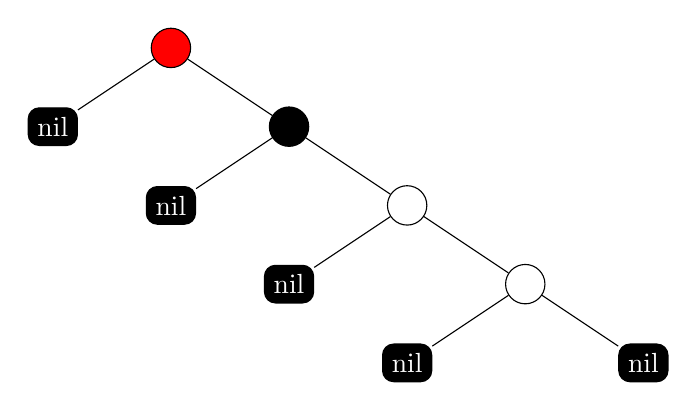
\begin{tikzpicture}
		[level 1/.style={level distance=1cm, sibling distance=3cm},
		level 2/.style={sibling distance=3cm},
		level 3/.style={sibling distance=3cm},
		level 4/.style={sibling distance=3cm},
		level 5/.style={sibling distance=3cm},
		level 6/.style={sibling distance=3cm},
		mynode/.style={
			circle,
			draw,
			minimum size=0.5cm
		},
		leaf/.style={rectangle,rounded corners,draw,fill=black,text=white,minimum height = 2mm, minimum width = 2mm}]
		\node[mynode,fill=red]{}
		child{
			node[leaf]{nil}
		}
		child
		{
			node[mynode,fill=black]{}
			child{
				node[leaf]{nil}
			}
			child{
				node[mynode]{}
				child{
					node[leaf]{nil}
				}
				child{
					node[mynode]{}
					child{
						node[leaf]{nil}
					}
					child{
						node[leaf]{nil}
					}
				}
			}
		};
	\end{tikzpicture}
} \\
\subfloat[Proviamo quindi a colorare la radice di nero. Il colore del figlio destro a questo punto non potrà essere che rosso se non si vuole squilibrare l'albero vioando il vincolo 5.]{
	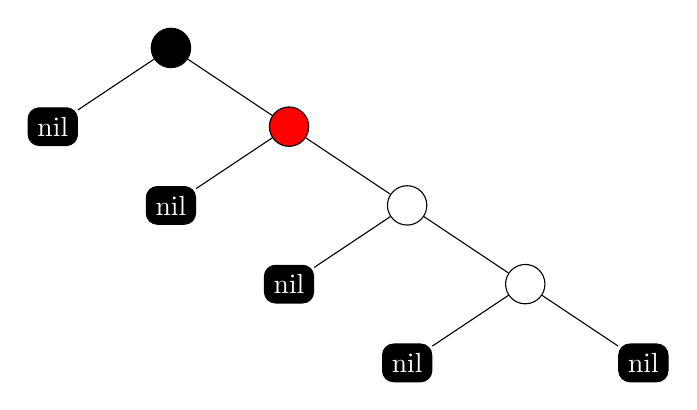
\begin{tikzpicture}
		[level 1/.style={level distance=1cm, sibling distance=3cm},
		level 2/.style={sibling distance=3cm},
		level 3/.style={sibling distance=3cm},
		level 4/.style={sibling distance=3cm},
		level 5/.style={sibling distance=3cm},
		level 6/.style={sibling distance=3cm},
		mynode/.style={
			circle,
			draw,
			minimum size=0.5cm
		},
		leaf/.style={rectangle,rounded corners,draw,fill=black,text=white,minimum height = 2mm, minimum width = 2mm}]
		\node[mynode,fill=black]{}
		child{
			node[leaf]{nil}
		}
		child
		{
			node[mynode,fill=red]{}
			child{
				node[leaf]{nil}
			}
			child{
				node[mynode]{}
				child{
					node[leaf]{nil}
				}
				child{
					node[mynode]{}
					child{
						node[leaf]{nil}
					}
					child{
						node[leaf]{nil}
					}
				}
			}
		};
\end{tikzpicture}} \qquad
\subfloat[Poiché si è colorato il secondo nodo di rosso, per il vincolo 4 il suo figlio dovrà essere nero. A questo punto però il vincolo 5 non è rispettato. Il percorso che dalla radice arriva alla foglia ha un solo nodo nero, mentre il percorso che arriva alla foglia successiva ne ha due.]{
	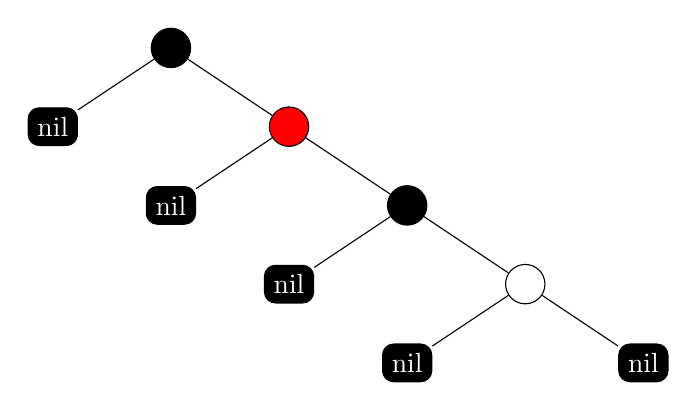
\begin{tikzpicture}
		[level 1/.style={level distance=1cm, sibling distance=3cm},
		level 2/.style={sibling distance=3cm},
		level 3/.style={sibling distance=3cm},
		level 4/.style={sibling distance=3cm},
		level 5/.style={sibling distance=3cm},
		level 6/.style={sibling distance=3cm},
		mynode/.style={
			circle,
			draw,
			minimum size=0.5cm
		},
		leaf/.style={rectangle,rounded corners,draw,fill=black,text=white,minimum height = 2mm, minimum width = 2mm}]
		\node[mynode,fill=black]{}
		child{
			node[leaf]{nil}
		}
		child
		{
			node[mynode,fill=red]{}
			child{
				node[leaf]{nil}
			}
			child{
				node[mynode,fill=black]{}
				child{
					node[leaf]{nil}
				}
				child{
					node[mynode]{}
					child{
						node[leaf]{nil}
					}
					child{
						node[leaf]{nil}
					}
				}
			}
		};
	\end{tikzpicture}
}
\caption{}
\end{figure}

\begin{center}
\begin{tikzpicture}[font=\tiny,scale=.7]
	\draw (0,0) [fill=primary!30]
	circle  (1cm)
	node {Alberi pieni}

	circle (2cm)
	node [align=center, anchor=north, yshift=1.2cm]{APB}

	circle (3cm)
	node [align=center, anchor=north, yshift=2cm]{Alberi AVL}

	circle (4cm)
	node [align=center, anchor=north, yshift=2.6cm]{Alberi R\&B}
	;
\end{tikzpicture}
\captionof{figure}{Relazione tra alberi perfettamente bilanciati, AVL e R\&B}\label{fig:gerarchia-alberi}
\end{center}

\subsection{Altezza di un albero rosso-nero}
I vincoli imposti sui nodi di un albero rosso-nero garantiscono che l'altezza dell'albero sia logaritmica sul numero dei nodi. In particolare, vincolare ogni nodo rosso ad avere solo figli neri e fissare l'altezza nera di ogni nodo a $bh(x)$, garantisce il contenimento dell'altezza dell'albero.


\begin{lemmabox}
Il numero di nodi interni di un sottoalbero radicato in $x$ è maggiore o uguale di $2^{bh(x)}-1$.
\end{lemmabox}
\begin{proof}
Si dimostra per induzione sull'altezza $h(x)$ dell'albero radicato in $x$:

\begin{itemize}
\item \textbf{Caso base:} $h(x)=0$. In questo caso, $x$ è una foglia esterna e, per definizione, non ha figli. Il numero di nodi interni è quindi $0$ e $2^{bh(x)}-1=2^0-1=0$.

\item \textbf{Passo induttivo:} $h(x)>0$. In questo caso, $x$ è un nodo interno e ha due figli: $s$ e $d$. Qual è la loro altezza nera? Distinguiamo due casi:
\begin{itemize}
\item $s$ è rosso. Allora $bh(s)=bh(x)\geq bh(x)-1$;
\item $s$ è nero. Allora $bh(s)=bh(x)-1\geq bh(x)-1$.
\end{itemize}
In maniera analoga abbiamo che $bh(d)\geq bh(x)-1$. Il numero dei nodi interni radicato in $x$ sarà pari a:
\begin{displaymath}
1 + \#_{int}(s) + \#_{int}(d)
\end{displaymath}
Poiché $h(s),h(d)<h(x)$ possiamo applicare l'ipotesi induttiva e ottenere:
\begin{displaymath}
\#_{int}(s)\geq 2^{bh(s)}-1 \geq 2^{bh(x)-1}-1
\end{displaymath}
e
\begin{displaymath}
\#_{int}(d)\geq 2^{bh(d)}-1 \geq 2^{bh(x)-1}-1
\end{displaymath}
Allora:
\begin{eqnarray*}
\#_{int}(x) &=& 1 + \#_{int}(s) + \#_{int}(d) \\
&\geq& 1 + 2 \cdot \bigl( 2^{bh(x)-1}-1\bigr) \\
&=& 2^{bh(x)}-1
\end{eqnarray*}
\end{itemize}
\end{proof}



\begin{teorbox}
L'altezza massima di un albero rosso-nero con $n$ nodi è al più $2\log(n+1)$.
\end{teorbox}
\begin{proof}
Sia $h$ l'altezza dell'albero. Per il vincolo 5, in ogni percorso da un nodo ad una foglia almeno la metà dei nodi sono neri. Allora, l'altezza nera dell'albero dovrà essere almeno $h/2$. Per il Lemma precedente, il numero di nodi interni dell'albero è almeno $2^{bh(T)}-1$. Allora:
\begin{center}
$\renewcommand\arraystretch{2}
\begin{array}{lll}
n & \geq 2^{bh(T)}-1 & \textcolor{gray}{\text{(per il Lemma precedente)}} \\
& \geq 2^{h/2}-1 & \textcolor{gray}{\text{(per il vincolo 5)}} \\
n+1 & \geq 2^{h/2} & \textcolor{gray}{\text{(spostando l'1 al primo membro)}} \\
\log(n+1) & \geq \frac{h}{2} & \textcolor{gray}{\text{(applicando il logaritmo)}} \\
2\log(n+1) & \geq h & \textcolor{gray}{\text{(moltiplicando per 2)}}
\end{array}$
\end{center}

In questo modo abbiamo trovato un limite superiore all'altezza dell'albero che dimostra il buon bilanciamento dell'albero.
\end{proof}

\begin{corolbox}
In un albero rosso nero le operazioni di ricerca, inserimento e cancellazione hanno un costo logaritmico sul numero dei nodi.
\end{corolbox}

\subsection{Inserimento in un albero rosso-nero}
L'inserimento in un albero rosso-nero è simile all'inserimento in un albero binario di ricerca. Esattamente come per gli alberi binari di ricerca, l'algoritmo di inserimento di un nodo $z$ in un albero rosso-nero cerca un cammino discendente dalla radice dell'albero fino al nodo $y$ che ne diventerà padre.

Una volta identificato il nodo $y$, il nodo $x$ viene inserito come figlio sinistro di $y$ se $z\rightarrow key \leq y \rightarrow key$, destro altrimenti. Tuttavia, nel caso di alberi rosso-neri bisognerà risolvere il problema di mantenere i vincoli imposti sui nodi dell'albero. In particolare, l'inserimento di un nodo potrebbe violare il vincolo 5, che impone che tutti i cammini da un qualsiasi nodo alle foglie sue discendenti abbiano lo stesso numero di nodi neri. Per questo motivo, l'inserimento di un nodo implicherebbe una sua colorazione di rosso. Tuttavia, questa colorazione potrebbe violare il vincolo 4, che impone che ogni nodo rosso abbia solo figli neri.

In generale, l'inserimento di un nodo potrebbe richiedere una serie di rotazioni e ricolorazioni dei nodi dell'albero. L'idea alla base per il ripristino della proprietà red-black, se necessario, al ritorno dalle chiamate ricorsive presenti nell'Algoritmo~\ref{lst:insert-rb} è la seguente: spostare le violazioni verso l'alto rispettando sempre il vincolo 5. Se la violazione arriva alla radice, la coloriamo di nero. Così facendo le operazioni di ripristino saranno necessarie solo quando due nodi consecutivi risultano rossi. In Figura~\ref{fig:rb-insertion} è mostrato un esempio di inserimento di un nodo in un albero rosso-nero.


\begin{lstlisting}[language=asd,caption={Insert-RB(T,k)},label=lst:insert-rb]
if not IS-NIL(T) then
if T@\rightarrow@ key < k then
T@\rightarrow@ right = Insert-RB(T@\rightarrow@ right,k)
T = Bilancia-Destra-RB(T)
else if T@\rightarrow@ key > k then
T@\rightarrow@ left = Insert-RB(T@\rightarrow@ left,k)
T = Bilancia-Sinistra-RB(T)
else
T = NewNodeRB(k)
T@\rightarrow@ color = RED
return T
\end{lstlisting}

\begin{center}
\begin{minipage}{.9\textwidth}
\centering
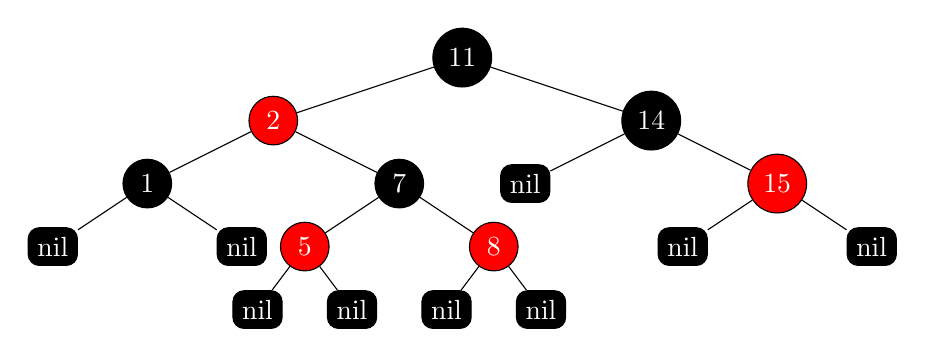
\begin{tikzpicture}
[scale=.8,
level 1/.style={level distance=1cm, sibling distance=6cm},
level 2/.style={sibling distance=4cm},
level 3/.style={sibling distance=3cm},
level 4/.style={sibling distance=1.5cm},
level 5/.style={sibling distance=1cm},
root/.style={circle,draw,fill=black,text=white,minimum size=0.5cm},
rednode/.style={circle,draw,fill=red,text=white,minimum size=0.5cm},
blacknode/.style={circle,draw,fill=black,text=white,minimum size=0.5cm},
leaf/.style={rectangle,rounded corners,draw,fill=black,text=white,minimum height = 2mm, minimum width = 2mm}]
\node[root]{11}
child{
  node[rednode]{2}
  child{
    node[blacknode]{1}
    child{
      node[leaf]{nil}
    }
    child{
      node[leaf]{nil}
    }
  }
  child{
    node[blacknode]{7}
    child{
      node[rednode]{5}
      child{
        node[leaf]{nil}
      }
      child{
        node[leaf]{nil}
      }
    }
    child{
      node[rednode]{8}
      child{
        node[leaf]{nil}
      }
      child{
        node[leaf]{nil}
      }
    }
  }
}
child{
  node[blacknode]{14}
  child{
    node[leaf]{nil}
  }
  child{
    node[rednode]{15}
    child{
      node[leaf]{nil}
    }
    child{
      node[leaf]{nil}
    }
  }
};
\end{tikzpicture}
\captionof{figure}{Albero dove inserire il nodo $z$\label{fig:rb-insertion}}
\end{minipage}
\\
\begin{minipage}{.9\textwidth}
\centering
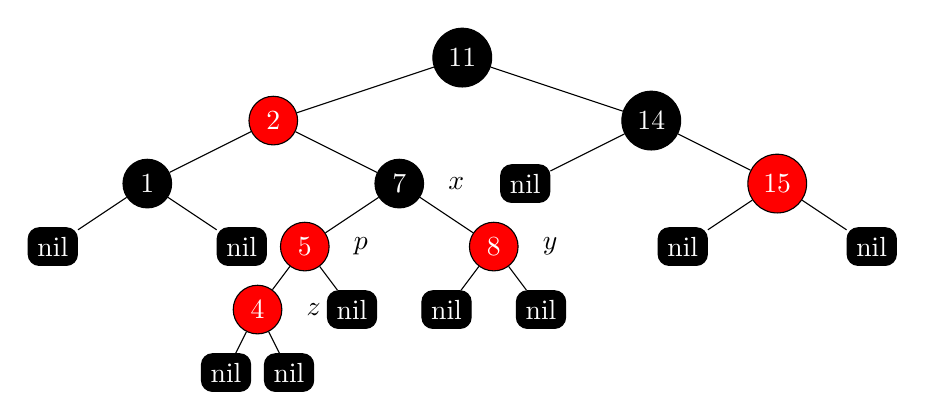
\begin{tikzpicture}
[scale=.8,
level 1/.style={level distance=1cm, sibling distance=6cm},
level 2/.style={sibling distance=4cm},
level 3/.style={sibling distance=3cm},
level 4/.style={sibling distance=1.5cm},
level 5/.style={sibling distance=1cm},
root/.style={circle,draw,fill=black,text=white,minimum size=0.5cm},
rednode/.style={circle,draw,fill=red,text=white,minimum size=0.5cm},
blacknode/.style={circle,draw,fill=black,text=white,minimum size=0.5cm},
leaf/.style={rectangle,rounded corners,draw,fill=black,text=white,minimum height = 2mm, minimum width = 2mm}]
\node[root]{11}
child{
  node[rednode]{2}
  child{
    node[blacknode]{1}
    child{
      node[leaf]{nil}
    }
    child{
      node[leaf]{nil}
    }
  }
  child{
    node[blacknode,name=x]{7}
    child{
      node[rednode,name=p]{5}
      child{
        node[rednode,name=z]{4}
        child{
          node[leaf]{nil}
        }
        child{
          node[leaf]{nil}
        }
      }
      child{
        node[leaf]{nil}
      }
    }
    child{
      node[rednode,name=y]{8}
      child{
        node[leaf]{nil}
      }
      child{
        node[leaf]{nil}
      }
    }
  }
}
child{
  node[blacknode]{14}
  child{
    node[leaf]{nil}
  }
  child{
    node[rednode]{15}
    child{
      node[leaf]{nil}
    }
    child{
      node[leaf]{nil}
    }
  }
};
\node[right,xshift=0.5cm] at (y) {$y$};
\node[right,xshift=0.5cm] at (x) {$x$};
\node[right,xshift=0.5cm] at (z) {$z$};
\node[right,xshift=0.5cm] at (p) {$p$};
\end{tikzpicture}
\captionof{figure}{L'inserimento del nodo $z$ causa una violazione del vincolo 4. Per risolvere il problema, il nodo $y$ viene ricolorato di nero e il suo genitore $x$ di rosso.}
\end{minipage}
\\
\begin{minipage}{.9\textwidth}
\centering
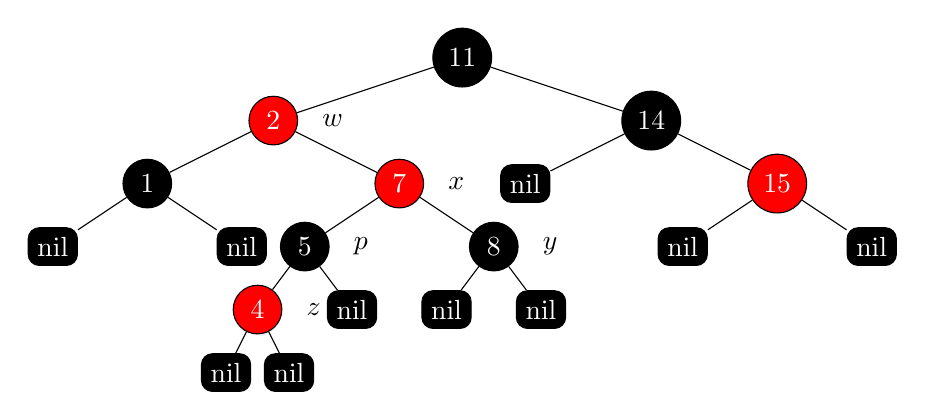
\begin{tikzpicture}
[scale=.8,
level 1/.style={level distance=1cm, sibling distance=6cm},
level 2/.style={sibling distance=4cm},
level 3/.style={sibling distance=3cm},
level 4/.style={sibling distance=1.5cm},
level 5/.style={sibling distance=1cm},
root/.style={circle,draw,fill=black,text=white,minimum size=0.5cm},
rednode/.style={circle,draw,fill=red,text=white,minimum size=0.5cm},
blacknode/.style={circle,draw,fill=black,text=white,minimum size=0.5cm},
leaf/.style={rectangle,rounded corners,draw,fill=black,text=white,minimum height = 2mm, minimum width = 2mm}]
\node[root]{11}
child{
  node[rednode,name=w]{2}
  child{
    node[blacknode]{1}
    child{
      node[leaf]{nil}
    }
    child{
      node[leaf]{nil}
    }
  }
  child{
    node[rednode,name=x]{7}
    child{
      node[blacknode,name=p]{5}
      child{
        node[rednode,name=z]{4}
        child{
          node[leaf]{nil}
        }
        child{
          node[leaf]{nil}
        }
      }
      child{
        node[leaf]{nil}
      }
    }
    child{
      node[blacknode,name=y]{8}
      child{
        node[leaf]{nil}
      }
      child{
        node[leaf]{nil}
      }
    }
  }
}
child{
  node[blacknode]{14}
  child{
    node[leaf]{nil}
  }
  child{
    node[rednode]{15}
    child{
      node[leaf]{nil}
    }
    child{
      node[leaf]{nil}
    }
  }
};
\node[right,xshift=0.5cm] at (y) {$y$};
\node[right,xshift=0.5cm] at (x) {$x$};
\node[right,xshift=0.5cm] at (z) {$z$};
\node[right,xshift=0.5cm] at (p) {$p$};
\node[right,xshift=0.5cm] at (w) {$w$};
\end{tikzpicture}
\captionof{figure}{In questo caso si procede con la ricolorazione del nodo $p$ e $y$ da rossi a neri mentre il nodo $x$ diventa nero per non alterare il numero di nodi neri. A  questo punto però si viola il vincolo 4 sul nodo $w$. Per risolvere lo sbilanciamento sarà quindi necessario cambiare il colore di $x$ e della radice violando così il vincolo 2 per evitare di violare il vincolo 5. Sarà quindi necessario procedere con una rotazione a destra per ripristinare il vincolo 2.}
\end{minipage}
\\
\begin{minipage}{.9\textwidth}
\centering
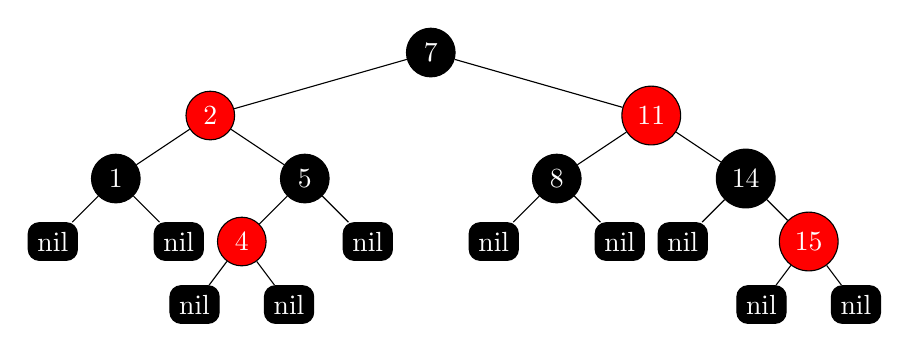
\begin{tikzpicture}
[scale=.8,
level 1/.style={level distance=1cm, sibling distance=7cm},
level 2/.style={sibling distance=3cm},
level 3/.style={sibling distance=2cm},
level 4/.style={sibling distance=1.5cm},
level 5/.style={sibling distance=1cm},
root/.style={circle,draw,fill=black,text=white,minimum size=0.5cm},
rednode/.style={circle,draw,fill=red,text=white,minimum size=0.5cm},
blacknode/.style={circle,draw,fill=black,text=white,minimum size=0.5cm},
leaf/.style={rectangle,rounded corners,draw,fill=black,text=white,minimum height = 2mm, minimum width = 2mm}
]
\node[root]{7}
child{
 node[rednode]{2}
 child{
  node[blacknode]{1}
  child{
   node[leaf]{nil}
  }
  child{
   node[leaf]{nil}
  }
 }
 child{
  node[blacknode]{5}
  child{
    node[rednode]{4}
    child{
      node[leaf]{nil}
    }
    child{
      node[leaf]{nil}
    }
  }
  child{
    node[leaf]{nil}
  }
 }
}
child{
  node[rednode]{11}
  child{
    node[blacknode]{8}
    child{
      node[leaf]{nil}
    }
    child{
      node[leaf]{nil}
    }
  }
  child{
    node[blacknode]{14}
    child{
      node[leaf]{nil}
    }
    child{
      node[rednode]{15}
      child{
        node[leaf]{nil}
      }
      child{
        node[leaf]{nil}
      }
    }
  }
};
\end{tikzpicture}
\captionof{figure}{Albero finale}
\end{minipage}
\end{center}

\subsubsection{Il bilanciamento del sottoalbero sinistro}
Come detto in precedenza, le operazioni di ripristino sono necessarie solo quando due nodi consecutivi sono rossi. Tra l'altro, se la radice dell'albero è sempre nera, non si presenterà mai la necessità di ribilanciare in un albero (o sottoalbero) di altezza minore di 3 in quanto non si possono verificare violazioni. A fronte di queste osservazioni possiamo distinguere tre casi possibili che possono scatenare una violazione del vincolo 4 a fronte dell'inserimento di un nuovo nodo $z$:
\begin{enumerate}
\item Lo zio $y$ di $z$ è rosso (Figura~\ref{fig:rb-insertion-case1});
\item Lo zio $y$ di $z$ è nero e $z$ è il figlio destro del figlio sinistro del padre $p$ (Figura~\ref{fig:rb-insertion-case2});
\item Lo zio $y$ di $z$ è nero e $z$ è il figlio sinistro del figlio sinistro del padre $p$ (Figura~\ref{fig:rb-insertion-case3}).
\end{enumerate}
L'Algoritmo \textsc{Bilancia-Sinistra-RB} (Algoritmo \ref{lst:bilancia-sx-rb}) sulla base di questi tre casi, provvede a ripristinare la proprietà red-black dell'albero. Con al massimo due rotazioni si riesce a risolvere il problema di bilanciamento. Questo però non deve stupire in quanto gli alberi rosso-neri sono più tolleranti degli alberi AVL e quindi è normale che ci siano meno rotazioni. Il vantaggio computazionale degli alberi rosso-neri rispetto agli alberi AVL sarà ben visibile nella fase di cancellazione. L'Algoritmo \textsc{Tipo-Violazione-Sinistra} (Algoritmo \ref{lst:tipo-violazione-sx}) calcola il tipo di violazione che si è verificata.

\begin{lstlisting}[language=asd,caption={Bilancia-Sinistra-RB(T)},label=lst:bilancia-sx-rb]
if ha_figlio(T@\rightarrow@left)
v = Tipo-Violazione_Sinistra(T@\rightarrow@left,T@\rightarrow@right)
case v of
1: T = Caso1(T)
2: T = Caso2(T)
3: T = Caso3(T)
return T
\end{lstlisting}


\begin{lstlisting}[language=asd,caption={Tipo-Violazione-Sinistra(S,D)},label=lst:tipo-violazione-sx]
v = 0
if S@\rightarrow@color = RED && D@\rightarrow@ color = RED then
if S@\rightarrow@left@\rightarrow@color = RED || S@\rightarrow@right@\rightarrow@color=R then
v = 1
else
if S@\rightarrow@color = RED && S@\rightarrow@right@\rightarrow@color = RED then
v = 2
else
if S@\rightarrow@left@\rightarrow@color = RED then
v = 3
return v
\end{lstlisting}

\begin{figure}[ht!]
\centering
\subfloat[Caso 1\label{fig:rb-insertion-case1}]
{
	\begin{tikzpicture}
		[
		level 1/.style={level distance=1cm, sibling distance=6cm},
		level 2/.style={sibling distance=4cm},
		level 3/.style={sibling distance=3cm},
		level 4/.style={sibling distance=1.5cm},
		level 5/.style={sibling distance=1cm},
		root/.style={circle,draw,fill=black,text=white,minimum size=0.5cm},
		rednode/.style={circle,draw,fill=red,text=white,minimum size=0.5cm},
		blacknode/.style={circle,draw,fill=black,text=white,minimum size=0.5cm},
		leaf/.style={rectangle,rounded corners,draw,fill=black,text=white,minimum height = 2mm, minimum width = 2mm},
		itria/.style={
			draw,
			shape border uses incircle,
			isosceles triangle,
			shape border rotate=90,
			yshift=-0.5cm
		},scale=.7]
		\node[blacknode]{C}
		child{
			node[rednode]{A}
			child{
				node[circle,fill=black]{}{node[itria]{}}
			}
			child{
				node[rednode,name=x]{B}
				child{
					node[circle,fill=black]{}{node[itria]{}}
				}
				child{
					node[circle,fill=black]{}{node[itria]{}}
				}
			}
		}
		child{
			node[rednode,name=y]{D}
			child{
				node[circle,fill=black]{}{node[itria]{}}
			}
			child{
				node[circle,fill=black]{}{node[itria]{}}
			}
		};
		\node[right,xshift=0.5cm] at (x) {$z$};
		\node[right,xshift=0.5cm] at (y) {$y$};
	\end{tikzpicture}
} \hfil
\subfloat[Caso 2\label{fig:rb-insertion-case2}]{
	\begin{tikzpicture}
		[
		level 1/.style={level distance=1cm, sibling distance=6cm},
		level 2/.style={sibling distance=4cm},
		level 3/.style={sibling distance=3cm},
		level 4/.style={sibling distance=1.5cm},
		level 5/.style={sibling distance=1cm},
		root/.style={circle,draw,fill=black,text=white,minimum size=0.5cm},
		rednode/.style={circle,draw,fill=red,text=white,minimum size=0.5cm},
		blacknode/.style={circle,draw,fill=black,text=white,minimum size=0.5cm},
		leaf/.style={rectangle,rounded corners,draw,fill=black,text=white,minimum height = 2mm, minimum width = 2mm},
		itria/.style={
			draw,
			shape border uses incircle,
			isosceles triangle,
			shape border rotate=90,
			yshift=-0.5cm
		},scale=.7]
		\node[blacknode]{C}
		child{
			node[rednode]{A}
			child{
				node[circle,fill=black]{}{node[itria]{}}
			}
			child{
				node[rednode,name=x]{B}
				child{
					node[circle,fill=black]{}{node[itria]{}}
				}
				child{
					node[circle,fill=black]{}{node[itria]{}}
				}
			}
		}
		child{
			node[circle,fill=black]{}{node[itria,fill=black,name=y]{}}
		};
		\node[right,xshift=0.5cm] at (x) {$z$};
		\node[right,xshift=0.5cm] at (y) {$y$};
	\end{tikzpicture}
}\\
\subfloat[Caso 3\label{fig:rb-insertion-case3}]{
	\begin{tikzpicture}
		[
		level 1/.style={level distance=1cm, sibling distance=6cm},
		level 2/.style={sibling distance=4cm},
		level 3/.style={sibling distance=3cm},
		level 4/.style={sibling distance=1.5cm},
		level 5/.style={sibling distance=1cm},
		root/.style={circle,draw,fill=black,text=white,minimum size=0.5cm},
		rednode/.style={circle,draw,fill=red,text=white,minimum size=0.5cm},
		blacknode/.style={circle,draw,fill=black,text=white,minimum size=0.5cm},
		leaf/.style={rectangle,rounded corners,draw,fill=black,text=white,minimum height = 2mm, minimum width = 2mm},
		itria/.style={
			draw,
			shape border uses incircle,
			isosceles triangle,
			shape border rotate=90,
			yshift=-0.5cm
		},scale=.7]
		\node[blacknode]{C}
		child{
			node[rednode]{B}
			child{
				node[rednode,name=x]{A}
				child{
					node[circle,fill=black]{}{node[itria]{}}
				}
				child{
					node[circle,fill=black]{}{node[itria]{}}
				}
			}
			child{
				node[circle,fill=black]{}{node[itria]{}}
			}
		}
		child{
			node[circle,fill=black]{}{node[itria,fill=black,name=y]{}}
		};
		\node[right,xshift=0.5cm] at (x) {$z$};
		\node[right,xshift=0.5cm] at (y) {$y$};
	\end{tikzpicture}
}
\caption{}
\end{figure}

\begin{minipage}{0.3\textwidth}
\begin{lstlisting}[language=asd,caption={Caso1(T)},label=lst:caso1-insert-rb]
T@\rightarrow@right@\rightarrow@color = BLACK
T@\rightarrow@left@\rightarrow@color = BLACK
T@\rightarrow@color = RED
return T
\end{lstlisting}
\end{minipage}\hfil
\begin{minipage}{0.35\textwidth}
\begin{lstlisting}[language=asd,caption={Caso2(T)},label=lst:caso2-insert-rb]
T@\rightarrow@left = Rotazione-Sx(T@\rightarrow@left)
T = Caso3(T)
return T
\end{lstlisting}
\end{minipage}\hfil
\begin{minipage}{0.3\textwidth}
\begin{lstlisting}[language=asd,caption={Caso3(T)},label=lst:caso3-insert-rb]
	T = Rotazione-Sx(T)
	T@\rightarrow@color = BLACK
	T@\rightarrow@right@\rightarrow@color = RED
	return T
\end{lstlisting}
\end{minipage}

\subsection{La cancellazione in un albero rosso-nero}
Analogamente ad altre operazioni elementari su un albero rosso-nero di $n$ nodi, la cancellazione di un nodo richiede un tempo logaritmico sul numero di nodi. A differenza però degli altri algoritmi di cancellazione, la cancellazione in un albero rosso-nero è più complessa in quanto richiede maggiori controlli per mantenere i vincoli imposti.



\begin{osservation}
Le operazioni di ripristino del bilanciamento sono necessarie solo quando il nodo cancellato è nero. Infatti, nel caso della cancellazione, non si può decidere a priori il colore del nodo da staccare. Qualora si dovesse eliminare un nodo nero siamo certi di aver modificato l'altezza nera dell'albero violando così il vincolo 5. Nel caso della cancellazione di un nodo rosso invece, si potrebbe al massimo aver avvicinato due nodi neri lungo un percorso ma la cosa non intacca alcun vincolo. Ripristinare questo vincolo però non è così complicato. L'idea alla base è quella di ignorare di aver violato il vincolo globale effettuando una \textbf{propagazione del colore nero} sul nodo che lo andrà a sostituire.
\end{osservation}


Se il nodo figlio era rosso allora è possibile colorarlo di nero, ma se questo fosse nero allora verrà colorato di un nuovo colore chiamato \textbf{doppio nero} (dal contributo che offre nel calcolo dell'altezza nera). In questo modo, il vincolo 5 verrà ripristinato. Tuttavia, questa introduzione di un terzo colore vìola il vincolo 1 che stabiliva che ogni nodo possa essere colorato o di rosso o di nero. Il problema per il ribilanciamento diventa quindi quello di eliminare i nodi doppio nero. L'algoritmo di cancellazione adotta una strategia simile a quella vista per la cancellazione negli alberi AVL.

\begin{minipage}{.45\textwidth}
\begin{lstlisting}[language=asd,caption={Delete-RB(T,k)},label=lst:delete-rb]
if !nil(T) then
if T@\rightarrow@ key < k then
T@\rightarrow@ right = Delete-RB(T@\rightarrow@ right,k)
T = Bilancia-Canc-Destra-RB(T)
else if T@\rightarrow@ key > k then
T@\rightarrow@ left = Delete-RB(T@\rightarrow@ left,k)
T = Bilancia-Canc-Sinistra-RB(T)
else
T = Delete-Root-RB(T)
return T
\end{lstlisting}

\begin{lstlisting}[language=asd,caption={Propagate-Black(T)},label=lst:propagate-black]
if T@\rightarrow@ color= RED then
T@\rightarrow@ color = BLACK
else
T@\rightarrow@ color = DOUBLE_BLACK
\end{lstlisting}
\end{minipage}
\hfil
\begin{minipage}{.4\textwidth}
\begin{lstlisting}[language=asd,caption={Delete-Root-RB(T)},label=lst:delete-root-rb]
if !nil(T) then
tmp = T
if nil(T@\rightarrow@ left) then
T = T @\rightarrow@ right
if tmp @\rightarrow@ color = BLACK then
  Propagate-Black(T)
else if nil(T@\rightarrow@ right) then
T = T@\rightarrow@ left
if tmp @\rightarrow@ color = BLACK then
  Propagate-Black(T)
else
tmp = Stacca-Min-RB(T@\rightarrow@ right,T)
T@\rightarrow@ key = tmp@\rightarrow@key
T = Bilancia-Canc-Destra-RB(T)
free(tmp)
return T
\end{lstlisting}
\end{minipage}

L'algoritmo \textsc{Stacca-Min-RB} è lo stesso visto per gli alberi AVL:
\begin{lstlisting}[language=asd,caption={Stacca-Min-RB(T,P)},label=lst:stacca-min-rb]
ret = nil
if !nil(P) && !nil(T) then
if !nil(T@\rightarrow@ left) then
ret = Stacca-Min-RB(T@\rightarrow@ left,T)
newT = Bilancia-Canc-Sinistra-RB(T)
else
ret = T
newT = T@\rightarrow@ right
if T @\rightarrow@ color = BLACK then
  Propagate-Black(newT)
if P @\rightarrow@ left = T then
  P @\rightarrow@ left = newT
else
  P @\rightarrow@ right = newT
return ret
\end{lstlisting}

\subsubsection{Il bilanciamento del sottoalbero sinistro}
Anche in questo caso, il bilanciamento del sottoalbero sinistro\footnote{Nel caso di sbilanciamento a destra si procede in modo simmetrico.} è simile a quello visto per gli alberi AVL. In particolare, l'algoritmo \textsc{Bilancia-Canc-Sinistra-RB} (Codice~\ref{lst:bilancia-sx-rb-del}) provvede a ripristinare la proprietà red-black dell'albero  eseguendo rotazioni e cambiamenti di colore. I vincoli che si possono violare a seguito della cancellazione di un nodo sono i seguenti:

\begin{itemize}
\item \textbf{Violazione del vincolo 3:} la radice può essere un nodo rosso;
\item \textbf{Violazione del vincolo 4:} se il padre e uno dei figli del nodo cancellato erano rossi;
\item \textbf{Violazione del vincolo 5:} altezza nera cambiata.
\end{itemize}

I casi che possono scatenare una violazione sono invece 4:
\begin{enumerate}
\item Il colore del fratello è rosso (Figura~\ref{fig:rb-deletion-case1});
\item I nipoti sono neri (Figura~\ref{fig:rb-deletion-case2});
\item Il nipote sinistro è rosso e il nipote destro è nero (Figura~\ref{fig:rb-deletion-case3});
\item Il nipote destro è rosso (Figura~\ref{fig:rb-deletion-case4}).
\end{enumerate}

\begin{lstlisting}[language=asd,caption={\textsc{Bilancia-Canc-Sinistra-RB}(T)},label=lst:bilancia-sx-rb-del]
if !nil(T@\rightarrow@ right) then
v = Violazione_Sx(T@\rightarrow@ left, T@\rightarrow@right)
case v of:
	1: T = Caso1(T)
 T = Bilancia-Canc-Sinistra(T@\rightarrow@left)
	2: T = Caso2(T)
	3: T = Caso3(T)
	4: T = Caso4(T)
return T
\end{lstlisting}

\begin{lstlisting}[language=asd,caption={\textsc{Violazione\_Sx}(X,W)},label=lst:violazione-sx]
	v = 0
	if X@\rightarrow@ color = DOUBLE-BLACK then
	if W@\rightarrow@ color = RED then
	v = 1
	else if W@\rightarrow@ right @\rightarrow@ color = BLACK && W @\rightarrow@ left @\rightarrow@ color = BLACK
	v = 2
	else if W@\rightarrow@ left @\rightarrow@ color = RED && W @\rightarrow@ right @\rightarrow@ color = BLACK
	v = 3
	else
	v = 4
	return v
\end{lstlisting}


Per comprendere il caso che effettua lo sbilanciamento si effettua un controllo sugli alberi del sottoalbero destro del padre del nodo doppio nero. Si ottiene così l'Algoritmo \textsc{Violazione-Sx} (Codice~\ref{lst:violazione-sx}). Analizziamo ora la gestione dei vari casi.

\paragraph{Caso 1:} il fratello è rosso. In questo caso, il fratello può essere colorato di nero e il padre può essere colorato di rosso. Successivamente si applica una rotazione destra sul fratello. A questo punto di determina una violazione sul nodo $E$ in quanto vede diminuita la sua altezza nera. Per risolvere la violazione del sottoalbero destro si ricolora la radice $D$ di nero ritrovandoci così nella situazione di una violazione del vincolo 5 nel sottoalbero sinistro. Quest'ultima violazione si risolve facilmente colorando il nodo $A$ di rosso. A questo punto ci si ritrova con un sottoalbero sbilanciato a sinistra di $A$ che è risolvibile riconducendosi al caso 2, 3 o 4.
\begin{lstlisting}[language=asd,caption={Caso1(T)},label=lst:caso1-rb-del]
T = Rotazione-Destra(T)
T@\rightarrow@ color = BLACK
T@\rightarrow@ right @\rightarrow@ color = RED
return T
\end{lstlisting}
\begin{figure}[ht!]
\centering
\subfloat[Configurazione iniziale\label{fig:rb-deletion-case1}]{
\begin{tikzpicture}
[
level 1/.style={level distance=1cm, sibling distance=6cm},
level 2/.style={sibling distance=4cm},
level 3/.style={sibling distance=3cm},
level 4/.style={sibling distance=1.5cm},
itria/.style={
draw,
dashed,
shape border uses incircle,
isosceles triangle,
shape border rotate=90,
yshift=-0.5cm,
fill=blue!25!white
},
root/.style={circle,draw,fill=black,text=white,minimum size=0.5cm},
rednode/.style={circle,draw,fill=red,text=white,minimum size=0.5cm},
blacknode/.style={circle,draw,fill=black,text=white,minimum size=0.5cm},
dbnode/.style={draw, circle, text centered, minimum size=0.5cm, fill=black, text=white, double,line width=2pt},
leaf/.style={rectangle,rounded corners,draw,fill=black,text=white,minimum height = 2mm, minimum width = 2mm},scale=.75
]
\node[root]{A}
child{
node[dbnode,name=b]{B}
child{
node[circle, fill=black]{} {node[itria]{}}
}
child{
node[circle, fill=black]{} {node[itria]{}}
}
}
child{
node[rednode,name=d]{D}
child{
node[blacknode]{C}
child{
  node[circle, fill=black]{} {node[itria]{}}
}
child{
  node[circle, fill=black]{} {node[itria]{}}
}
}
child{
node[blacknode]{E}
child{
  node[circle, fill=black]{} {node[itria]{}}
}
child{
  node[circle, fill=black]{} {node[itria]{}}
}
}
};
%draw arrow from d to b
\draw[->,red,>=stealth',shorten >=1pt,auto,thick] (d) to [bend right=45] (b);
\end{tikzpicture}
}\hfil
\subfloat[Configurazione dopo la rotazione\label{fig:rb-deletion-case12}]{
\begin{tikzpicture}
[
level 1/.style={level distance=1cm, sibling distance=6cm},
level 2/.style={sibling distance=4cm},
level 3/.style={sibling distance=3cm},
level 4/.style={sibling distance=1.5cm},
itria/.style={
draw,
dashed,
shape border uses incircle,
isosceles triangle,
shape border rotate=90,
yshift=-0.5cm,
fill=blue!25!white
},
root/.style={circle,draw,fill=black,text=white,minimum size=0.5cm},
rednode/.style={circle,draw,fill=red,text=white,minimum size=0.5cm},
blacknode/.style={circle,draw,fill=black,text=white,minimum size=0.5cm},
dbnode/.style={draw, circle, text centered, minimum size=0.5cm, fill=black, text=white, double,line width=2pt},
leaf/.style={rectangle,rounded corners,draw,fill=black,text=white,minimum height = 2mm, minimum width = 2mm},scale=.75
]
\node[rednode]{D}
child{
node[blacknode]{A}
child{
node[dbnode,name=b]{B}
child{
  node[circle, fill=black]{} {node[itria]{}}
}
child{
  node[circle, fill=black]{} {node[itria]{}}
}
}
child{
node[blacknode]{C}
child{
  node[circle, fill=black]{} {node[itria]{}}
}
child{
  node[circle, fill=black]{} {node[itria]{}}
}
}
}
child{
node[blacknode]{E}
child{
node[circle, fill=black]{} {node[itria]{}}
}
child{
node[circle, fill=black]{} {node[itria]{}}
}
};
\end{tikzpicture}
}\hfil
\subfloat[Configurazione dopo la ricolorazione\label{fig:rb-deletion-case13}]{
\begin{tikzpicture}
[
level 1/.style={level distance=1cm, sibling distance=6cm},
level 2/.style={sibling distance=4cm},
level 3/.style={sibling distance=3cm},
level 4/.style={sibling distance=1.5cm},
itria/.style={
draw,
dashed,
shape border uses incircle,
isosceles triangle,
shape border rotate=90,
yshift=-0.5cm,
fill=blue!25!white
},
root/.style={circle,draw,fill=black,text=white,minimum size=0.5cm},
rednode/.style={circle,draw,fill=red,text=white,minimum size=0.5cm},
blacknode/.style={circle,draw,fill=black,text=white,minimum size=0.5cm},
dbnode/.style={draw, circle, text centered, minimum size=0.5cm, fill=black, text=white, double,line width=2pt},
leaf/.style={rectangle,rounded corners,draw,fill=black,text=white,minimum height = 2mm, minimum width = 2mm},scale=.75]
\node[rednode]{D}
child{
node[rednode]{A}
child{
node[dbnode,name=b]{B}
child{
  node[circle, fill=black]{} {node[itria]{}}
}
child{
  node[circle, fill=black]{} {node[itria]{}}
}
}
child{
node[blacknode]{C}
child{
  node[circle, fill=black]{} {node[itria]{}}
}
child{
  node[circle, fill=black]{} {node[itria]{}}
}
}
}
child{
node[blacknode]{E}
child{
node[circle, fill=black]{} {node[itria]{}}
}
child{
node[circle, fill=black]{} {node[itria]{}}
}
};
\end{tikzpicture}
}
\caption{Caso 1}
\end{figure}

\paragraph{Caso 2:} il fratello è nero e i nipoti sono neri. In questo caso, il fratello può essere colorato di rosso e il doppio nero può essere propagato al padre. Ciò significa che il nodo $A$ diventerà doppio nero se prima già era nero, semplicemente nero altrimenti (vedi Figura~\ref{fig:rb-deletion-case22}). Questo caso è il più semplice in quanto non richiede alcuna rotazione. Nel caso in cui il nodo $A$ sia diventato doppio nero sarà necessario effettuare un nuovo ribilanciamento. L'Algoritmo \textsc{Caso2} (Codice~\ref{lst:caso2-rb-del}) si occupa di gestire questa situazione.
\begin{lstlisting}[language=asd,caption={Caso2(T)},label=lst:caso2-rb-del]
T @rightarrow@ right @\rightarrow@ color = RED
T @\rightarrow@ left @\rightarrow@ color = BLACK
Propagate-Black(T)
return T
\end{lstlisting}
\begin{figure}[ht!]
\centering
\subfloat[Configurazione iniziale\label{fig:rb-deletion-case2}]{
\begin{tikzpicture}
[
level 1/.style={level distance=1cm, sibling distance=6cm},
level 2/.style={sibling distance=4cm},
level 3/.style={sibling distance=3cm},
level 4/.style={sibling distance=1.5cm},
itria/.style={
draw,
dashed,
shape border uses incircle,
isosceles triangle,
shape border rotate=90,
yshift=-0.5cm,
fill=blue!25!white
},
root/.style={circle,draw,fill=black,text=white,minimum size=0.5cm},
rednode/.style={circle,draw,fill=red,text=white,minimum size=0.5cm},
blacknode/.style={circle,draw,fill=black,text=white,minimum size=0.5cm},
dbnode/.style={draw, circle, text centered, minimum size=0.5cm, fill=black, text=white, double,line width=2pt},
leaf/.style={rectangle,rounded corners,draw,fill=black,text=white,minimum height = 2mm, minimum width = 2mm},scale=.75
]
\node[draw,circle, text=black, fill=white]{A}
child{
node[dbnode]{B}
child{
node[circle, fill=black]{} {node[itria]{}}
}
child{
node[circle, fill=black]{} {node[itria]{}}
}
}
child{
node[blacknode]{D}
child{
node[blacknode]{C}
child{
  node[circle, fill=black]{} {node[itria]{}}
}
child{
  node[circle, fill=black]{} {node[itria]{}}
}
}
child{
node[blacknode]{E}
child{
  node[circle, fill=black]{} {node[itria]{}}
}
child{
  node[circle, fill=black]{} {node[itria]{}}
}
}
};
\end{tikzpicture}
}\hfil
\subfloat[Ribilanciamento caso 2\label{fig:rb-deletion-case22}]{
\begin{tikzpicture}
[
level 1/.style={level distance=1cm, sibling distance=6cm},
level 2/.style={sibling distance=4cm},
level 3/.style={sibling distance=3cm},
level 4/.style={sibling distance=1.5cm},
itria/.style={
draw,
dashed,
shape border uses incircle,
isosceles triangle,
shape border rotate=90,
yshift=-0.5cm,
fill=blue!25!white
},
root/.style={circle,draw,fill=black,text=white,minimum size=0.5cm},
rednode/.style={circle,draw,fill=red,text=white,minimum size=0.5cm},
blacknode/.style={circle,draw,fill=black,text=white,minimum size=0.5cm},
dbnode/.style={draw, circle, text centered, minimum size=0.5cm, fill=black, text=white, double,line width=2pt},
leaf/.style={rectangle,rounded corners,draw,fill=black,text=white,minimum height = 2mm, minimum width = 2mm},scale=.75
]
\node[draw,circle, text=black, fill=white]{A}
child{
node[blacknode]{B}
child{
node[circle, fill=black]{} {node[itria]{}}
}
child{
node[circle, fill=black]{} {node[itria]{}}
}
}
child{
node[rednode]{D}
child{
node[blacknode]{C}
child{
  node[circle, fill=black]{} {node[itria]{}}
}
child{
  node[circle, fill=black]{} {node[itria]{}}
}
}
child{
node[blacknode]{E}
child{
  node[circle, fill=black]{} {node[itria]{}}
}
child{
  node[circle, fill=black]{} {node[itria]{}}
}
}
};
\end{tikzpicture}
}
\caption{Caso 2}
\end{figure}

\paragraph{Caso 3:} il fratello è nero, il nipote sinistro è rosso e il nipote destro è nero. In questo caso, ruotiamo il fratello con il suo figlio sinistro, cambiamo il colore del padre e quello del figlio destro. L'Algoritmo \textsc{Caso3} (Codice~\ref{lst:caso3-rb-del}) si occupa di gestire questa situazione. Alla fine di questa procedura il sottoalbero sinistro del nodo $C$ introduce una violazione di tipo 5 che si risolve ricolorando i nodi. Alla fine della procedura ci si riconduce al caso 4.
\begin{lstlisting}[language=asd,caption={Caso3(T)},label=lst:caso3-rb-del]
T @rightarrow@ right =  Rotazione-Sinistra(T @\rightarrow@ right)
T @rightarrow@ right @\rightarrow@ color = BLACK
T @\rightarrow@ right @\rightarrow@ right @\rightarrow@ color = RED
T = Caso4(T)
return T
\end{lstlisting}
\begin{figure}[ht!]
\centering
\subfloat[Configurazione iniziale e senso della rotazione\label{fig:rb-deletion-case3}]{
\begin{tikzpicture}
	[
	level 1/.style={level distance=1cm, sibling distance=6cm},
	level 2/.style={sibling distance=4cm},
	level 3/.style={sibling distance=3cm},
	level 4/.style={sibling distance=1.5cm},
	itria/.style={
		draw,
		dashed,
		shape border uses incircle,
		isosceles triangle,
		shape border rotate=90,
		yshift=-0.5cm,
		fill=blue!25!white
	},
	root/.style={circle,draw,fill=black,text=white,minimum size=0.5cm},
	rednode/.style={circle,draw,fill=red,text=white,minimum size=0.5cm},
	blacknode/.style={circle,draw,fill=black,text=white,minimum size=0.5cm},
	dbnode/.style={draw, circle, text centered, minimum size=0.5cm, fill=black, text=white, double,line width=2pt},
	leaf/.style={rectangle,rounded corners,draw,fill=black,text=white,minimum height = 2mm, minimum width = 2mm},scale=.75
	]
	\node[draw,circle, text=black, fill=white]{A}
	child{
		node[dbnode]{B}
		child{
			node[circle, fill=black]{} {node[itria]{}}
		}
		child{
			node[circle, fill=black]{} {node[itria]{}}
		}
	}
	child{
		node[blacknode]{D}
		child{
			node[rednode,name=c]{C}
			child{
				node[circle, fill=black]{} {node[itria]{}}
			}
			child{
				node[circle, fill=black]{} {node[itria]{}}
			}
		}
		child{
			node[blacknode,name=e]{E}
			child{
				node[circle, fill=black]{} {node[itria]{}}
			}
			child{
				node[circle, fill=black]{} {node[itria]{}}
			}
		}
	};
%Draw arrow from c to e
\draw[->,red,>=stealth',shorten >=1pt,auto,thick] (c) to [bend left=45] (e);
\end{tikzpicture}
}\hfil
\subfloat[Configurazione dopo la prima rotazione\label{fig:rb-deletion-case32}]{
\begin{tikzpicture}
	[
	level 1/.style={level distance=1cm, sibling distance=6cm},
	level 2/.style={sibling distance=4cm},
	level 3/.style={sibling distance=3cm},
	level 4/.style={sibling distance=1.5cm},
	itria/.style={
		draw,
		dashed,
		shape border uses incircle,
		isosceles triangle,
		shape border rotate=90,
		yshift=-0.5cm,
		fill=blue!25!white
	},
	root/.style={circle,draw,fill=black,text=white,minimum size=0.5cm},
	rednode/.style={circle,draw,fill=red,text=white,minimum size=0.5cm},
	blacknode/.style={circle,draw,fill=black,text=white,minimum size=0.5cm},
	dbnode/.style={draw, circle, text centered, minimum size=0.5cm, fill=black, text=white, double,line width=2pt},
	leaf/.style={rectangle,rounded corners,draw,fill=black,text=white,minimum height = 2mm, minimum width = 2mm},scale=.75
	]
	\node[draw,circle, text=black, fill=white]{A}
	child{
		node[dbnode]{B}
		child{
			node[circle, fill=black]{} {node[itria]{}}
		}
		child{
			node[circle, fill=black]{} {node[itria]{}}
		}
	}
	child{
		node[rednode]{C}
  child{
    node[circle, fill=black]{} {node[itria]{}}
  }
  child{
    node[blacknode]{D}
    child{
      node[circle, fill=black]{} {node[itria]{}}
    }
    child{
      node[blacknode,name=e]{E}
      child{
        node[circle, fill=black]{} {node[itria]{}}
      }
      child{
        node[circle, fill=black]{} {node[itria]{}}
      }
    }
  }
	};
\end{tikzpicture}
} \\
\subfloat[Configurazione finale dopo la ricolorazione\label{fig:rb-deletion-case33}]{
\begin{tikzpicture}
	[
	level 1/.style={level distance=1cm, sibling distance=6cm},
	level 2/.style={sibling distance=4cm},
	level 3/.style={sibling distance=3cm},
	level 4/.style={sibling distance=1.5cm},
	itria/.style={
		draw,
		dashed,
		shape border uses incircle,
		isosceles triangle,
		shape border rotate=90,
		yshift=-0.5cm,
		fill=blue!25!white
	},
	root/.style={circle,draw,fill=black,text=white,minimum size=0.5cm},
	rednode/.style={circle,draw,fill=red,text=white,minimum size=0.5cm},
	blacknode/.style={circle,draw,fill=black,text=white,minimum size=0.5cm},
	dbnode/.style={draw, circle, text centered, minimum size=0.5cm, fill=black, text=white, double,line width=2pt},
	leaf/.style={rectangle,rounded corners,draw,fill=black,text=white,minimum height = 2mm, minimum width = 2mm},scale=.75
	]
	\node[draw,circle, text=black, fill=white]{A}
	child{
		node[dbnode]{B}
		child{
			node[circle, fill=black]{} {node[itria]{}}
		}
		child{
			node[circle, fill=black]{} {node[itria]{}}
		}
	}
	child{
		node[blacknode]{C}
  child{
    node[circle, fill=black]{} {node[itria]{}}
  }
  child{
    node[rednode]{D}
    child{
      node[circle, fill=black]{} {node[itria]{}}
    }
    child{
      node[blacknode,name=e]{E}
      child{
        node[circle, fill=black]{} {node[itria]{}}
      }
      child{
        node[circle, fill=black]{} {node[itria]{}}
      }
    }
  }
	};
\end{tikzpicture}
}
\caption{Caso 3}
\end{figure}

\paragraph{Caso 4:} il fratello è nero e il nipote destro è rosso. In questo caso eseguiamo una rotazione del padre del nodo doppio nero con il fratello. Dopo la rotazione il nodo $B$ continua a pesare come un doppio nero, di conseguenza procediamo cambiando i colori opportunamente ed eliminando il nero in più sul nodo. L'Algoritmo \textsc{Caso4} (Codice~\ref{lst:caso4-rb-del}) si occupa di gestire questa situazione.
\begin{lstlisting}[language=asd,caption={Caso4(T)},label=lst:caso4-rb-del]
T = Rotazione-Sinistra(T)
T @\rightarrow@ right @\rightarrow@ color = T @\rightarrow@ color
T @\rightarrow@ color = T @\rightarrow@ left @\rightarrow@ color
T @\rightarrow@ left @\rightarrow@ color = BLACK
T @\rightarrow@ left @\rightarrow@ left @\rightarrow@ color = BLACK
return T
\end{lstlisting}
\begin{figure}[ht!]
\centering
\subfloat[Configurazione iniziale\label{fig:rb-deletion-case4}]{
\begin{tikzpicture}
[
level 1/.style={level distance=1cm, sibling distance=6cm},
level 2/.style={sibling distance=4cm},
level 3/.style={sibling distance=3cm},
level 4/.style={sibling distance=1.5cm},
itria/.style={
	draw,
	dashed,
	shape border uses incircle,
	isosceles triangle,
	shape border rotate=90,
	yshift=-0.5cm,
	fill=blue!25!white
},
root/.style={circle,draw,fill=black,text=white,minimum size=0.5cm},
rednode/.style={circle,draw,fill=red,text=white,minimum size=0.5cm},
blacknode/.style={circle,draw,fill=black,text=white,minimum size=0.5cm},
dbnode/.style={draw, circle, text centered, minimum size=0.5cm, fill=black, text=white, double,line width=2pt},
leaf/.style={rectangle,rounded corners,draw,fill=black,text=white,minimum height = 2mm, minimum width = 2mm},scale=.75
]
\node[circle,draw,fill=white,text=black]{A}
child{
	node[dbnode,name=b]{B}
	child{
		node[circle, fill=black]{} {node[itria]{}}
	}
	child{
		node[circle, fill=black]{} {node[itria]{}}
	}
}
child{
	node[blacknode,name=d]{D}
	child{
		node[circle,draw,fill=white, text=black]{C}
		child{
			node[circle, fill=black]{} {node[itria]{}}
		}
		child{
			node[circle, fill=black]{} {node[itria]{}}
		}
	}
	child{
		node[rednode]{E}
		child{
			node[circle, fill=black]{} {node[itria]{}}
		}
		child{
			node[circle, draw,fill=black]{} {node[itria]{}}
		}
	}
};
\draw[->,red,>=stealth',shorten >=1pt,auto,thick] (d) to [bend right=45] (b);
\end{tikzpicture}
}\\
\subfloat[Configurazione dopo la rotazione\label{fig:rb-deletion-case42}]{
\begin{tikzpicture}
[
level 1/.style={level distance=1cm, sibling distance=6cm},
level 2/.style={sibling distance=4cm},
level 3/.style={sibling distance=3cm},
level 4/.style={sibling distance=1.5cm},
itria/.style={
	draw,
	dashed,
	shape border uses incircle,
	isosceles triangle,
	shape border rotate=90,
	yshift=-0.5cm,
	fill=blue!25!white
},
root/.style={circle,draw,fill=black,text=white,minimum size=0.5cm},
rednode/.style={circle,draw,fill=red,text=white,minimum size=0.5cm},
blacknode/.style={circle,draw,fill=black,text=white,minimum size=0.5cm},
dbnode/.style={draw, circle, text centered, minimum size=0.5cm, fill=black, text=white, double,line width=2pt},
leaf/.style={rectangle,rounded corners,draw,fill=black,text=white,minimum height = 2mm, minimum width = 2mm},scale=.75
]
\node[root]{D}
child{
	node[circle,draw,fill=white,text=black]{A}
	child{
		node[dbnode]{B}
  child{
    node[circle, fill=black]{} {node[itria]{}}
  }
  child{
    node[circle, fill=black]{} {node[itria]{}}
  }
	}
	child{
		node[circle,draw,fill=white,text=black]{C}
  child{
    node[circle, fill=black]{} {node[itria]{}}
  }
  child{
    node[circle, fill=black]{} {node[itria]{}}
  }
	}
}
child{
	node[rednode]{E}
	child{
  node[circle, fill=black]{} {node[itria]{}}
}
child{
  node[circle, draw,fill=black]{} {node[itria]{}}
}
};
\end{tikzpicture}
}
\\
\subfloat[Configurazione dopo la ricolorazione\label{fig:rb-deletion-case43}]{
\begin{tikzpicture}
[
level 1/.style={level distance=1cm, sibling distance=6cm},
level 2/.style={sibling distance=4cm},
level 3/.style={sibling distance=3cm},
level 4/.style={sibling distance=1.5cm},
itria/.style={
	draw,
	dashed,
	shape border uses incircle,
	isosceles triangle,
	shape border rotate=90,
	yshift=-0.5cm,
	fill=blue!25!white
},
root/.style={circle,draw,fill=black,text=white,minimum size=0.5cm},
rednode/.style={circle,draw,fill=red,text=white,minimum size=0.5cm},
blacknode/.style={circle,draw,fill=black,text=white,minimum size=0.5cm},
dbnode/.style={draw, circle, text centered, minimum size=0.5cm, fill=black, text=white, double,line width=2pt},
leaf/.style={rectangle,rounded corners,draw,fill=black,text=white,minimum height = 2mm, minimum width = 2mm},scale=.75
]
\node[circle,draw, fill=white,text=black]{D}
child{
	node[blacknode]{A}
	child{
		node[blacknode]{B}
  child{
    node[circle, fill=black]{} {node[itria]{}}
  }
  child{
    node[circle, fill=black]{} {node[itria]{}}
  }
	}
	child{
		node[circle,draw,fill=white,text=black]{C}
  child{
    node[circle, fill=black]{} {node[itria]{}}
  }
  child{
    node[circle, fill=black]{} {node[itria]{}}
  }
	}
}
child{
	node[blacknode]{E}
	child{
  node[circle, fill=black]{} {node[itria]{}}
}
child{
  node[circle, draw,fill=black]{} {node[itria]{}}
}
};
\end{tikzpicture}
}
\caption{Caso 4}
\end{figure}

\chapter{Ricorsione ed iterazione}\label{cap:ricorsione}
\section{La ricorsione}
In informatica il concetto di ricorsione è estremamente importante in quanto permette di ottenere spesso una descrizione chiara e concisa degli algoritmi. Diciamo che un algoritmo è \textit{ricorsivo} se figurano in esso delle procedure ricorsive, ovvero procedure che invocano, direttamente o indirettamente, sé stesse. Come abbiamo visto fino a questo momento, questa tipologia di algoritmi costituiscono il metodo più naturale di risoluzione di un problema in quanto sono facili da comprendere e analizzare. Infatti:
\begin{itemize}
	\item La correttezza di un programma ricorsivo si dimostra facilmente utilizzando il \textit{principio di induzione};
	\item Il calcolo della complessità temporale di un algoritmo ricorsivo si riduce alla soluzione delle equazioni di ricorrenza (come si vedrà nel Capitolo \ref{cap:ricorrenze}).
\end{itemize}
Affinché un algoritmo ricorsivo non continui a girare all'infinito deve avere le seguenti proprietà:
\begin{enumerate}
	\item Devono esistere dei criteri, detti \textbf{criteri di base} (o anche \textit{casi base}), per i quali la procedura non richiami sé stessa;
	\item Ogni volta che la procedura chiama sé stessa, essa deve essere più vicina ai criteri di base.
\end{enumerate}
Una procedura ricorsiva dotata di queste due proprietà si dice \textbf{ben definita}.

Il prodotto dei numeri interi positivi da $1$ a $n$ compresi prende il nome di ``fattoriale di $n$'' e si indica con il simbolo $n!$:
\begin{equation}
	n! = 1 \cdot 2 \cdot 3 \cdot \cdots (n-2) \cdot (n-1) \cdot n
\end{equation}
Per definizione si pone $0!=1$ quindi è possibile definire una funzione ben definita per tutti i numeri naturali. Si dimostra per induzione che:
\begin{equation}
	n! = \begin{cases}
		1 & \text{se } n=0\\
		n \cdot(n-1)!& \text{se } n>0
	\end{cases}
\end{equation}
Questa definizione di $n!$ è ricorsiva, infatti quando si usa $(n-1)!$ si sta eseguendo una ``chiamata'' alla funzione stessa. Questa definizione è ben definita in quanto il valore $n!$ è esplicitamente assegnato quando $n=0$ ed inoltre il valore $n!$ è definito in funzione di un valore più piccolo di $n$, più vicino quindi al valore di base $0$. Per calcolare, ad esempio, $4!$ saranno necessari nove passaggi. Infatti:
\begin{enumerate}
	\item $4!=4 \cdot 3!$
	\item \hspace{1cm} $3!=3 \cdot 2!$
	\item \hspace{2cm} $2!=2 \cdot 1!$
	\item \hspace{3cm} $1!=1 \cdot 0!$
	\item \hspace{4.5cm} $0!=1$
	\item \hspace{3cm} $1!=1 \cdot 1 = 1$
	\item \hspace{2cm} $2!=2 \cdot 1 = 2$
	\item \hspace{1cm} $3!=3 \cdot 2 = 6$
	\item $4!=4 \cdot 6 = 24$
\end{enumerate}


Vediamo ora una procedura che calcola il fattoriale:
	\begin{lstlisting}[language=asd,caption={\textsc{factorial\_rec}(N)},label=lst:factR]
		if N = 0 then
			fact = 1
		else
			x = factorial_rec(n-1)
			fact = N * x
		return fact;
	\end{lstlisting}

Non tutti i linguaggi di programmazione, però, supportano la ricorsione\footnote{Pascal e Cobol ad esempio non la permettono.}. La ricorsione, infatti, non è un meccanismo proprio del calcolatore il quale, come si è detto quando si è parlato di macchine astratte (vedi Sezione \ref{sez:Turing}), ha un insieme limitato di operazioni ed opera mediante assegnazioni e salti\footnote{Infatti in un calcolatore non è neanche definito il concetto di ciclo ed iterazione.}.

I linguaggi che permettono la ricorsione utilizzano in fase di esecuzione uno \textbf{stack} per tenere traccia della sequenza di chiamata delle varie procedure ricorsive. In testa a tale stack è sempre presente il \textit{record di attivazione} contenente il \textbf{contesto} della procedura correntemente attiva. Tale contesto comprende:
\begin{itemize}
	\item le variabili locali alla procedura;
	\item i parametri ad essa passati;
	\item l'indirizzo di ritorno, ovvero il contenuto del \textit{program counter} nel momento in cui la procedura è stata invocata.
\end{itemize}

Quando una procedura è invocata viene posto sulla pila un nuovo record di attivazione. Ciò indipendentemente dal fatto che siano già presenti nella pila altri record di attivazione relativi alla stessa procedura. Per questo motivo la ricorsione è molto dispendiosa in termini di memoria. Più in avanti vedremo alcuni esempi di algoritmi ricorsivi che non richiedono l'utilizzo di uno stack.

\section{La traduzione da ricorsivo ad iterativo}
\subsection{La memoria di lavoro}
Come abbiamo visto, la ricorsione è un meccanismo che non è proprio del calcolatore. Per questo motivo, quando si scrive un programma ricorsivo, il compilatore deve tradurlo in un programma iterativo. Alla base di questa traduzione c'è il concetto di \textbf{memoria di lavoro} che è una memoria ausiliaria che viene utilizzata per salvare i dati necessari al calcolo di una procedura ricorsiva. In particolare, la memoria di lavoro è costituita da uno \textbf{stack} che viene utilizzato per salvare i \textbf{parametri formali} delle varie chiamate ricorsive. Ogni volta che è necessario eseguire una sottochiamata ricorsiva ci si avvale della memoria di lavoro per salvare i parametri formali della procedura corrente per poterli poi recuperare al ritorno dalla chiamata ricorsiva. In questo modo, la memoria di lavoro permette di simulare la ricorsione mediante iterazione.

\subsection{Uno schema generale per la traduzione}
\subsubsection{Il ciclo while}
La traduzione di un algoritmo ricorsivo in un algoritmo iterativo richiede un approccio basato su un grande ciclo \texttt{while} il quale gestisce al suo interno le due fasi principali di una chiamata ricorsiva: l'\textbf{inizializzazione} di una nuova chiamata ricorsiva e il \textbf{ripristino} dei dati precedentemente utilizzati al \textit{ritorno} di una queste ultime.  Per capire quale fase bisogna gestire ci avvaliamo di una variabile booleana \texttt{start}\footnote{Negli esempi presenti nel capitolo capiterà di sostituire tale variabile con una vera e propria condizione sui parametri attuali.} che assume valore \texttt{true} quando siamo nella fase di \textit{inizializzazione} di una nuova chiamata ricorsiva e \texttt{false} quando siamo nella fase di \textit{ripresa} di una chiamata sospesa.

Oltre alla condizione sulla variabile \texttt{start}, è necessario controllare anche lo \textbf{stato dello stack}. Infatti, se lo stack è vuoto significa che \textit{non ci sono chiamate ricorsive sospese} e quindi non è necessario effettuare alcuna ripresa e si può procedere fino alla fine dell'algoritmo. In caso contrario sarà necessario \textit{ripristinare il contesto della chiamata ricorsiva sospesa} per eseguire le varie sottochiamate e proseguire con l'esecuzione dell'algoritmo.

\subsubsection{Il punto di ritorno: la variabile last}
Al ritorno da una chiamata ricorsiva bisogna cercare di capire il punto dal quale riprendere l'esecuzione della chiamata precedentemente sospesa. Per fare ciò è necessario individuare il cosiddetto \textbf{punto di ritorno}, ovvero l'istruzione che segue immediatamente la chiamata ricorsiva appena terminata. In generale, un modo per discriminare il punto di ritorno a fronte di più chiamate ricorsive è quello di utilizzare una variabile \texttt{last} la quale, \textit{ogni volta che si termina una chiamata ricorsiva}, viene aggiornata con il valore del parametro attuale che sarà sicuramente diverso dai corrispettivi delle altre sottochiamate ricorsive (in caso contrario, infatti, si avrebbero chiamate ridondanti e si finirebbe in un loop).

È possibile quindi delineare uno schema generale per la traduzione di un algoritmo ricorsivo in uno puramente iterativo come mostrato in Figura \ref{fig:schema}.

\begin{center}
	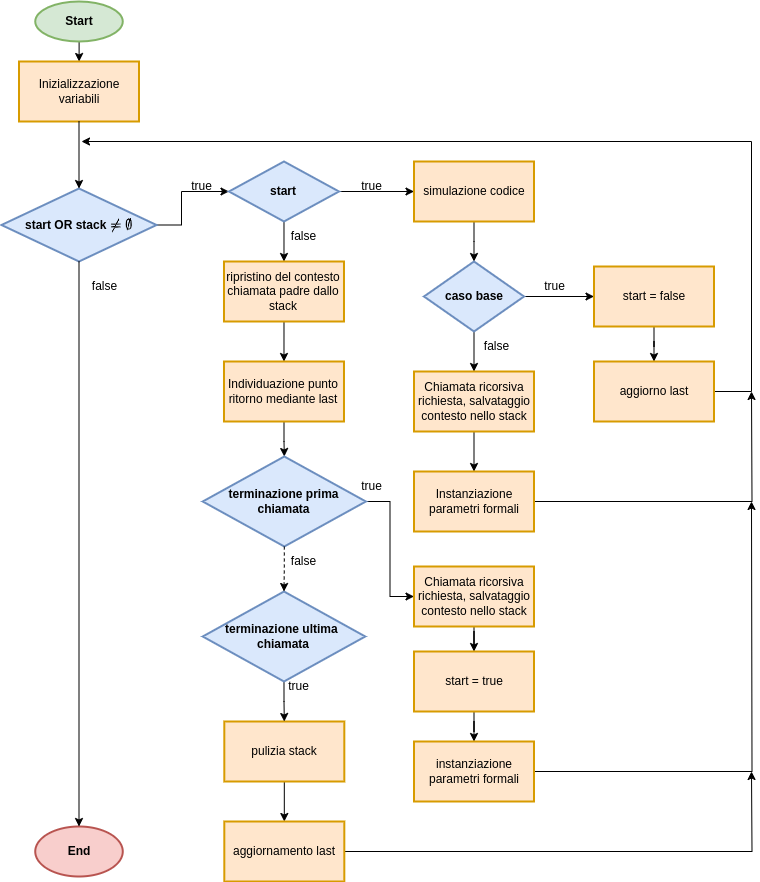
\includegraphics[scale=.6]{res/schema_traduzione}
	\captionof{figure}{Schema algoritmo iterativo che simula algoritmo ricorsivo}\label{fig:schema}
\end{center}


\subsection{La funzione fattoriale}
Osservando l'algoritmo \ref{lst:factR} notiamo che si effettuano nuove chiamate ricorsive ogni qualvolta la variabile \texttt{N} è maggiore o uguale a zero. Per questo motivo possiamo pensare di porre come condizione di loop nel ciclo \texttt{while} il controllo \texttt{cn $\geq$ n}.

Per poter ripristinare il contesto della chiamata padre, è necessario salvare in memoria i parametri formali della procedura ricorsiva. Nel caso della funzione fattoriale, per simulare l'inizio di una chiamata ricorsiva, è necessario verificare se il parametro \texttt{N} è uguale a \texttt{0} e, in caso affermativo, assegnare il valore \texttt{1} alla variabile \texttt{ret}.

Nel caso in cui \texttt{N} sia diverso da \texttt{0} è necessario eseguire una nuova chiamata ricorsiva. Per permetterlo è necessario innanzitutto salvare nello stack il valore corrente  di \texttt{N} e assegnare a \texttt{cn} (\textit{current n}) il valore \texttt{N-1} (\textbf{instanziazione parametri formali}). Sarà quindi necessario un unico stack per salvare il valore di \texttt{N}. Non è necessario salvare il valore di \texttt{fact} in quanto questo viene calcolato al ritorno dalla chiamata ricorsiva.

Chiaramente, una volta arrivati al caso base il valore \texttt{cn} sarà uguale a \texttt{-1} ma lo stack non sarà vuoto e sarà necessario effettuare nuove iterazioni per svuotarlo per ottenere il valore finale. Si ha così un primo esempio di traduzione di un algoritmo ricorsivo in un algoritmo iterativo:

\begin{lstlisting}[caption={Traduzione iterativa della funzione fattoriale},language=asd]
cn = n
stack = NIL
while (cn >= 0 || stack != NIL) do
	if cn >= 0 then
		// caso base
		if cn = 0 then
			r = 1
			ret = r
			cn = -1
		// avvio sottochiamata
		else
			// salvataggio contesto
			stack = push(stack, cn)
			// aggiorno il parametro per la sottochiamata
			cn = cn - 1
	// ritorno da sottochiamata
	else
		// ripristino contesto
		cn = top(stack)
		x = ret
		r = cn * x
		stack = pop(stack)
		ret = r
		cn = -1
return ret
\end{lstlisting}

\subsection{L'esempio del MergeSort}
Consideriamo l'algoritmo di ordinamento \texttt{Merge Sort}. Questo è un algoritmo di ordinamento ricorsivo basato sul concetto del ``divide et impera''. La sua idea principale consiste nel dividere un array non ordinato in due metà, ordinare ciascuna metà separatamente, e infine combinare le due metà ordinate in un unico array ordinato. L'algoritmo opera ricorsivamente fino a quando l'array non può essere più diviso, e poi procede a combinare le parti ordinate.

\begin{lstlisting}[caption={\textsc{MergeSort}(A,p,r)},language=asd,label={lst:mergeSortR}]
if p<r then
	q = (p+r)/2
	MergeSort(A,p,q)
	MergeSort(A,q+1,r)
	Merge(A,p,q,r)
\end{lstlisting}

Notiamo fin da subito che l'algoritmo \texttt{MergeSort} richiama se stesso due volte. Quando un compilatore traduce un programma scritto in un linguaggio di alto livello in un linguaggio di basso livello, come il linguaggio macchina, non può utilizzare la ricorsione in quanto non esiste in esso. Il compilatore deve quindi tradurre la ricorsione in iterazione.

Nell'algoritmo \ref{lst:mergeSortR} compaiono quattro variabili: \texttt{p, r, q, A}. Durante la fase di traduzione in iterazione, notiamo però che solo le variabili \texttt{p}, \texttt{q} ed \texttt{r} vengono modificate. La variabile \texttt{A} rappresenta un puntatore alla prima cella dell'array da ordinare e che quindi non cambia mai mentre la variabile \texttt{q} viene calcolata in ogni sottochiamata dati i valori correnti di \texttt{p} ed \texttt{r} (salvati nelle variabili \texttt{cp} e \texttt{cr}), per questo motivo non sarebbe necessario memorizzare la variabile \texttt{q} ma ciò nonostante utilizzeremo tre stack, uno per ogni variabile \texttt{p, q, r}.

Per discriminare il punto di ritorno, avendo a che fare con due chiamate ricorsive, utilizzeremo la variabile \texttt{last} che verrà aggiornata ogni volta che si termina una chiamata ricorsiva. Infatti, ciascuna sottochiamata assume parametri formali diversi e ogni volta che termina deve comunicare al padre il valore del suo terzo parametro per poter proseguire con l'esecuzione. Per questo motivo, la variabile \texttt{last} conterrà il valore della variabile \texttt{cr}. Al ritorno da ciascuna sottochiamata, basterà quindi controllare se il valore di \texttt{last} è uguale al valore di \texttt{cr} per capire se si è terminata la prima o la seconda sottochiamata. Se, al termine di una iterazione, \texttt{last} è uguale a \texttt{q} allora sicuramente si sta tornando dalla terminazione della prima chiamata ricorsiva. Se invece \texttt{last} è uguale a \texttt{cr} allora non sarà necessario effettuare nuove chiamate ricorsive e si può procedere fino alla fine dell'algoritmo.

\begin{lstlisting}[caption={\textsc{MergeSort\_Iter}(A,p,r)},language=asd,label={lst:mergeSortI}]
cp = p
cr = r
stackR = NIL
stackP = NIL
stackQ = NIL
start = true
while (start || stackR != NIL) do
	if start then
		if cp < cr then
			// simulazione codice fino alla prima chiamata ricorsiva
			q = (cp+cr)/2
			// avvio prima sottochiamata, salvataggio contesto
			stackR = push(stackR, cr)
			stackP = push(stackP, cp)
			stackQ = push(stackQ, q)
			// aggiornamento parametri formali
			cr = q
		// simulazione terminazione, la chiamata padre potrebbe essere stata sospesa
		else
			last = cr
			start = false
	else
		// ripristino contesto
		cr = top(stackR)
		cp = top(stackP)
		q = top(stackQ)
		// individuazione punto di ritorno
		if last @$\neq$@ cr then
			cp = q + 1
			start = true
		else
		// fine della seconda sottochiamata, terminazione chiamata corrente e pulizia record
			Merge(A,cp,q,cr)
			stackR = pop(stackR)
			stackP = pop(stackP)
			stackQ = pop(stackQ)
			last = cr
\end{lstlisting}

\subsection{La funzione di Fibonacci}
Sia $Fib(n)$ la funzione che restituisce l'$n$-esimo numero della successione di Fibonacci. Tale valore viene calcolato come segue:
\begin{equation}\label{eq:fibo}
	Fib(n) = \begin{cases}
		0 & \text{se } n =0\\
		1 & \text{se } n = 1\\
		Fib(n-1)+Fib(n-1) & \text{se } n>1
	\end{cases}
\end{equation}
Possiamo, quindi, definire un algoritmo ricorsivo che segua in maniera diretta l'equazione \ref{eq:fibo}.
\begin{lstlisting}[language=asd,caption={\textsc{Fib}(n)},label=lst:fibR]
	if n @$\leq$@ 1 then
		r = n
	else
		x = Fib(n-1)
		r = x+ Fib(n-2)
	return r
\end{lstlisting}

Per eseguire la traduzione dell'algoritmo \ref{lst:fibR} in uno iterativo, è necessario utilizzare uno stack per salvare i valori precedentemente calcolati e che verranno utilizzati per calcolare il valore finale. L'algoritmo richiama se stesso due volte, per questo motivo utilizzeremo la variabile \texttt{last} per discriminare il punto di ritorno, se \texttt{last} è diverso  da \texttt{cn - 2} allora si sta tornando dalla prima chiamata ricorsiva, altrimenti si sta tornando dalla seconda chiamata ricorsiva.

Si ha quindi:
\begin{lstlisting}[language=asd,caption={\textsc{Fib\_Iter}(n)},label=lst:fibI]
cn = n
stack = NIL
stack_X = NIL
start = true
while (start || stack @$\neq$@ NIL) do
	if start then
		// Controllo del caso base
		if cn <= 1 then
			r = cn
			ret = r
			last = cn
			start = false
		else
			// Salvataggio del contesto
			stack = push(stack, cn)
			cn = cn - 1
	else
		// Ripristino del contesto
		cn = top(stack)
		// Individuazione del punto di ritorno
		if last @$\neq$@ cn - 2 then
			// Operazioni da eseguire al termine della prima sottochiamata
			x = ret
			stack_X = push(stack_X,x)
			cn = cn - 2
			start = true
		else
			// Operazioni da eseguire al termine della seconda sottochiamata
			x = top(stack_X)
			r = x + ret
			// Ripulisco lo stack
			stack = pop(stack)
			// Aggiornamento last
			ret = r
			last = cn
return r
\end{lstlisting}
\subsection{Un algoritmo generico}
Consideriamo l'algoritmo \ref{lst:algoR}:
\begin{lstlisting}[language=asd,caption={\textsc{Algo}(A,p,r,k)},label=lst:algoR]
ret = 0
z = 0
if (p <= r) then
	q = (p+r)/2
	if (k = A[q]) then
		z = A[q]
	ret = z + Algo(A,q+1,r,k)
	if (ret > 0) then
		ret = ret + Algo(A,p,q-1,k)
return ret
\end{lstlisting}

Per tradurre l'algoritmo \ref{lst:algoR} in uno iterativo è bene osservare che qualsiasi variabile che viene scritta prima e letta dopo una chiamata ricorsiva deve essere salvata all'interno di uno stack apposito. Per questo motivo si useranno tre stack per salvare i valori di \texttt{p}, \texttt{q} e \texttt{ret}. Inoltre, è necessario utilizzare la variabile \texttt{last} per discriminare il punto di ritorno. Infatti, l'algoritmo richiama se stesso due volte, per questo motivo è necessario utilizzare la variabile \texttt{last} per capire se si sta tornando dalla prima o dalla seconda chiamata ricorsiva. In questo caso, il valore che viene sempre modificato ad ogni chiamata ricorsiva e che contraddistingue ciascuna chiamata è \texttt{p}. Per questo motivo, la variabile \texttt{last} conterrà il valore di \texttt{cp}. Si ha quindi:

\begin{lstlisting}[language=asd,caption={\textsc{Algo\_Iter}(A,p,r,k)}]
start = true
cp = p
cr = r
stackP = stackQ = stackRet = NIL
while (start || stackP @$\neq$@ NIL) do
	if (start) then
		// Istruzioni fino alla prima chiamata ricorsiva
		ret = 0
		z = 0
		if (cp <= cr) then
			q = (cp+cr)/2
			if (k = A[q]) then
				z = A[q]
			// Salvataggio del contesto
			stackP = push(stackP,cp)
			stackQ = push(stackQ,q)
			cp = q+1
		else
			// Simulazione terminazione chiamata
			result = ret
			last = cp
			start = false
	else
		// Ripristino contesto
		cp = top(stackP)
		q = top(stackQ)
		// Individuazione punto di ritorno
		if (cp @$\neq$@ last) then
			// Impostazione del valore della variabile z
			if(k=A[q]) then
				z =A[q]
			else
				z = 0
			// Prima istruzione successiva al ritorno dalla prima chiamata
			ret = z + result
			if(ret>0) then
				// Inizializzazione seconda chiamata, salvataggio del contesto
				stackRet = push(stackRet, ret)
				cr = q-1
				start = true
			else
				// Terminazione chiamata
				result = ret
				last = cp
				// Pulizia stack
				stackP=pop(stackP)
				stackQ=pop(stackQ)
		else
			// Ritorno dalla seconda chiamata
			ret = top(stackRet)
			ret = ret + result
			// Terminazione chiamata
			result = ret
			last = cp
			// Pulizia stack
			stackP = pop(stackP)
			stackQ = pop(stackQ)
			stackRet = pop(stackRet)
return ret
\end{lstlisting}
\section{Gli algoritmi ricorsivi negli alberi binari}
Quando abbiamo visto lo schema generale per la traduzione di un algoritmo ricorsivo si è visto come discriminare tra le due fasi di un algoritmo ricorsivo. Ricapitolando:
\begin{itemize}
	\item L'inizializzazione di nuova chiamata ricorsiva avviene quando la condizione \texttt{start } risulta vera;
	\item La ripresa del controllo dopo  la terminazione di una sottochiamata  avviene invece quando \texttt{start = false} e quando ci sono ancora elementi all'interno dei vari stack (\texttt{ stack $\neq \varnothing$}).
\end{itemize}
Tra le varie assunzioni fatte, inoltre, si è adoperata una variabile \texttt{last} aggiornata al valore del parametro attuale modificato da restituire alla chiamata padre per distinguere il punto di ritorno. In questa sezione osserveremo però che \textit{questo meccanismo non funziona nel caso degli algoritmi che operano sugli alberi binari}.

\subsection{L'algoritmo Search}
Consideriamo un algoritmo di ricerca in un albero binario generico.
\begin{lstlisting}[language=asd,caption={\textsc{Search}(T,k)}]
	if T@$\neq$@ NIL then
		if T@$\rightarrow$@ key @$\neq$@ k then
			ret = Search(T@$\rightarrow$@ left,k)
			if ret @$\neq$@ NIL then
				ret = Search(T @$\rightarrow$@ right,k)
	return ret
\end{lstlisting}

In questo caso, l'unico parametro che viene modificato nel corso delle varie sottochiamate ricorsive è rappresentato dalla testa del sottoalbero sul quale viene eseguita la ricerca. Non ha senso inizializzare uno stack per la variabile \texttt{ret} in quanto questa viene sempre calcolata ad ogni sottochiamata ed il vecchio valore non viene più utilizzato.

Come già anticipato, non è possibile utilizzare la strategia adottata finora per l'individuazione del punto di ritorno. Infatti, quando viene effettuata una chiamata su un nodo foglia si avrà che sia \texttt{last = ct = T $\rightarrow$ left} che \texttt{last = ct = T $\rightarrow$ right} sono uguali a \texttt{NIL}, quindi al ritorno dalle sottochiamate ricorsive sarebbe impossibile discriminare quale delle due chiamate si è appena conclusa.
\begin{center}
	\begin{tikzpicture}
		[font=\ttfamily,minimum height=.7cm]
		\node (Key) [rectangle,draw,minimum width=3cm] {\texttt{key}};
		\node (LeftChild) [rectangle,draw,anchor=north west,minimum width=1.5cm] at (Key.south west) {\texttt{left}};
		\node (RightChild) [rectangle,draw,anchor=north east,minimum width=1.5cm] at (Key.south east) {\texttt{right}};
		\node[name=n1,yshift=-1cm] at (LeftChild.south west){NIL};
		\node[name=n2,yshift=-1cm] at (RightChild.south east){NIL};
		\draw[->, thick](RightChild) -- (n2);
		\draw[->,thick](LeftChild)--(n1);
	\end{tikzpicture}
\end{center}
Per risolvere tale problema, osserviamo che la prima sottochiamata viene effettuata sempre sul sottoalbero sinistro quindi, se ad un certo punto dell'iterazione si vede che \texttt{last} è uguale a \texttt{NIL} vorrà dire che la chiamata appena terminata è quella di sinistra. Si ha quindi:
\begin{lstlisting}[caption={\textsc{Search\_Iter}(T,k)},language=asd]
ct = T
start = true
stackT = NIL
while (start || stackT @$\neq$@ NIL) do
	ret = ct
	if (start) then
		if (ct @$\rightarrow$@ key @$\neq$@ k) then
			// Salvataggio contesto
			stackT = push(stackT, ct)
			ct = ct @$\rightarrow$@ left
		else
			result = ret
			start = false
			last = ct
		else
			// Ripristino contesto
			ct = top(stackT)
			// Individuazione punto di ritorno
			if (last = ct @$\rightarrow$@ left && ct @$\rightarrow$@ right @$\neq$@ NIL) then
				ret = result
				if (ret = NIL) then
					ct = ct @$\rightarrow$@ right
					start = true
				else
					stackT = pop(stackT)
					result = ret
					last = ct
			else
				stackT = pop(stackT)
				result = ret
				last = ct
return ret
\end{lstlisting}

\subsection{L'algoritmo PrintTree}
Consideriamo adesso l'algoritmo che si occupa di stampare in post-ordine le chiavi dei nodi presenti in un albero binario:
\begin{lstlisting}[language=asd,label=lst:print_tree,caption={\textsc{PrintTree}(T)}]
	if T@$\neq$@ NIL then
		PrintTree(T@$\rightarrow$@ left)
		PrintTree(T@$\rightarrow$@ right)
		print(T@$\rightarrow$@ key)
\end{lstlisting}
Dal momento che le varie sottochiamate vengono applicate su sottoalberi diversi sarà necessario salvare in uno stack il riferimento al sottoalbero corrente nel momento in cui si effettua una chiamata ricorsiva. Si ha quindi:
\begin{lstlisting}[language=asd,caption={\textsc{PrintTree\_Iter}(T)}]
ct = T
start = true
stackT = NIL
while (start || stackT @$\neq$@ NIL) do
	if (start) then
		if (ct @$\neq$@ NIL) then
			// Salvataggio contesto
			stackT = push(stackT, ct)
			ct = ct @$\rightarrow$@ left
		else
			last = ct
			start = false
	else
		ct = top(stackT)
		// Individuazione punto di ritorno
		if (last = ct @$\rightarrow$@ left && ct @$\rightarrow$@ right @$\neq$@ NIL) then
			ct = ct @$\rightarrow$@ right
			start = true
		// Fine della seconda sottochiamata
		else
			print(ct @$\rightarrow$@ key)
			stackT = pop(stackT)
			last = ct
\end{lstlisting}
\section{La ricorsione in coda}
Come detto all'inizio del capitolo la ricorsione può richiedere una grande allocazione di memoria dato dallo stack dei record di attivazione per ognuna delle chiamate effettuate col rischio di incorrere in overflow di memoria.

\begin{example}
	Si può dimostrare, ad esempio, che nell'esecuzione dell'Algoritmo \textsc{Fib}$(n)$ (Algoritmo \ref{lst:fibR}) le chiamate \textsc{Fib}$(0)$ e \textsc{Fib}$(1)$ sono calcolati \textsc{Fib}$(n+1)$ volte. Nella computazione di \textsc{Fib}$(29)$ sono chiamati $832040 = $ \textsc{Fib}$(30)$ volte.
	\begin{center}
		\begin{tikzpicture}
			[every node/.style={rectangle, draw},
			level 1/.style={sibling distance=4cm},
			level 2/.style={sibling distance =2cm}]
			\node{$fib(n)$}
			child
			{
				node{$fib(n-1)$}
				child
				{
					node[fill=blue!75!black]{$fib(n-2)$}
				}
				child
				{
					node[fill=green!75!black]{$fib(n-2)$}
				}
			}
			child
			{
				node[fill=blue!75!black]{$fib(n-2)$}
				child
				{
					node[fill=green!75!black]{$fib(n-2)$}
				}
				child
				{
					node{$fib(n-4)$}
				}
			};
		\end{tikzpicture}
	\end{center}
\end{example}
Per evitare tale dispendio di memoria è possibile pensare di costruire una ricorsione definita in modo tale che nel caso ricorsivo l'\textbf{ultima operazione} da eseguire è la chiamata ricorsiva. Infatti, se l'ultima istruzione effettuata nella funzione chiamante risulta la chiamata ricorsiva, allora non è necessario specificare alcun indirizzo di ritorno nella funzione chiamante ed è possibile sostituire tale valore con l'indirizzo di ritorno della funzione principale da cui la ricorsiva veniva chiamata.

Consideriamo ad esempio l'algoritmo di ricerca sugli alberi binari di ricerca:
\begin{lstlisting}[language=asd,caption={\textsc{SearchABR}(T,k)}]
ret = T
if T @$\neq$@ NIL then
	if (T@$\rightarrow$@ key < k) then
		ret = SearchABR(T @$\rightarrow$@ right, k)
	else if (T@$\rightarrow$@ key > k) then
		ret = SearchABR(T @$\rightarrow$@ left, k)
return ret
\end{lstlisting}
In questa situazione si osserva che non è assolutamente necessario salvare il contesto degli antenati (le chiamate padri) in quanto il calcolo della variabile \texttt{ret} avviene in modo indipendente dai suoi precedenti. Non è pertanto necessaria alcuna memoria aggiuntiva in quanto la ricerca di un nodo si riduce, nel caso degli alberi binari di ricerca, alla discesa lungo un percorso ben definito.

\begin{lstlisting}[language=asd,caption={\textsc{SearchABR\_Iter}(T,k)}]
ret = T
while (ret @$\neq$@ NIL && ret @$\rightarrow$@ key @$\neq$@ k) do
	if (ret @$\rightarrow$@ key < k) then
		ret = ret @$\rightarrow$@ right
	else
		ret = ret @$\rightarrow$@ left
return ret
\end{lstlisting}

La categoria di algoritmi per i quali non serve uno stack per il salvataggio del contesto adoperano una tipologia di ricorsione che prende il nome di \textbf{ricorsione in coda}. Sintatticamente, la ricorsione in coda corrisponde ad un algoritmo che effettua una sola chiamata ricorsiva senza dover effettuare infine una risalita\footnote{Per convenzione gli stack evolvono verso il basso.} lungo lo stack di attivazione per il recupero del contesto precedente. In modo del tutto analogo è possibile riscrivere l'algoritmo ricorsivo \ref{lst:factR} per il calcolo del fattoriale $n!$ in modo tale che effettui una ricorsione in coda:
\begin{lstlisting}[language=asd,caption={\textsc{Fattoriale\_Iter}(N)}]
t = 1
while (n>0) do
	t = t*n
	n = n-1
return t
\end{lstlisting}

Come si può osservare, non è necessario alcuno stack per il salvataggio del contesto delle chiamate interrotte in quanto il calcolo del risultato altro non fa che utilizzare le variabili condivise nel corso dell'iterazione: \texttt{t} per il calcolo del risultato e il parametro attuale \texttt{n} che viene decrementato di iterazione in iterazione.

\chapter{Il metodo divide et impera: gli alberi di ricorsione}\label{cap:ricorrenze}

\section{Le ricorrenze}
Nel Capitolo \ref{cap:ricorsione} si è definito il concetto di ricorsione e di metodo divide et impera. Nel metodo \textbf{divide et impera} un problema viene risolto in modo \textbf{ricorsivo}, applicando tre passi ad ogni livello di ricorsione.
\begin{itemize}
	\item \textbf{Divide:} questo passo divide il problema in un certo numero di sottoproblemi che sono istanze più piccole dello \textit{stesso problema}.
	\item \textbf{Impera:} i sottoproblemi vengono risolti in modo \textit{ricorsivo}. Quando si è arrivati ad una dimensione sufficientemente piccola delle istanze, queste vengono risolte direttamente.
	\item \textbf{Combina:} le soluzioni dei sottoproblemi vengono combinate per generare la soluzione del problema generale.
\end{itemize}

Quando i sottoproblemi sono abbastanza grandi da essere risolti ricorsivamente si ha il cosiddetto \textbf{caso ricorsivo}. Una volta che i sottoproblemi diventano sufficientemente piccoli da non richiedere ricorsione si dice che la ricorsione ``ha toccato il fondo'' e che si è raggiunto il \textbf{caso base}. Da notare come tutto questo procedimento abbia come base teorica il \textbf{principio di induzione}.

\dfn{Ricorrenza}{
	Una \textbf{ricorrenza} è un'equazione, detta anche \textbf{equazione di ricorrenza}, che descrive una funzione in termini del suo valore di input con input più piccoli. Una ricorrenza per il tempo di esecuzione di un algoritmo divide et impera si basa sui tre passi del paradigma di base.
}

\begin{example}
	Supposto $T(n)$ sia il tempo di esecuzione di un problema di dimensione $n$. Se la dimensione del problema è sufficientemente piccola, per esempio $n \leq c$ per qualche costante $c$, la soluzione diretta richiede un tempo costante, che si indica con $\Theta(1)$. Supposto che la suddivisione del problema generi $a$ sottoproblemi e che la dimensione di ciascun sottoproblema sia $1/b$ volte la dimensione del problema originale allora servirà tempo $T(n/b)$ per risolvere un sottoproblema di dimensione $n/b$ e quindi, per risolverne $a$, servirà un tempo $a \cdot T(n/b)$. Se impieghiamo un tempo $D(n)$ per dividere il problema in sottoproblemi e un tempo $C(n)$ per combinare le soluzioni dei sottoproblemi nella soluzione del problema originale, si ottiene la ricorrenza:
\begin{displaymath}
	T(n)=
	\begin{cases}
		\Theta(1) & \text{se } n\leq c \\
		aT(n/b)+D(n)+C(n) & \text{negli altri casi}
	\end{cases}
\end{displaymath}
\end{example}

I sottoproblemi non devono necessariamente essere espressi mediante una frazione costante della dimensione del problema iniziale. Ad esempio, una versione ricorsiva della ricerca lineare all'interno di un array non creerebbe un solo sottoproblema in quanto dovrebbe richiamare sé stessa, fino a quando l'elemento da ricercare non è stato trovato, su un array contenente un elemento in meno rispetto alla chiamata padre. La ricorrenza che si ottiene sarà allora:
\begin{displaymath}
	T(n) = \begin{cases}
		\Theta(1) & \text{se } n=1\\
		T(n-1)+\Theta(1) & \text{se } n>1
	\end{cases}
\end{displaymath}

\section{Metodo dell'albero di ricorsione}
In un \textbf{albero di ricorsione} ogni nodo rappresenta il costo di un singolo sottoproblema da qualche parte nell'insieme delle chiamate ricorsive di funzione. Sommando i costi all'interno di ogni livello dell'albero è possibile determinare il costo totale di un algoritmo ricorsivo. Questa analisi prende il nome di \textbf{metodo dell'albero di ricorsione}.

\begin{example}
	Si consideri l'equazione:
\begin{equation}\label{eqricorrenza1}
	T(n)=
	\begin{cases}
		\Theta(1) & \text{se } n \leq 1 \\
		2T(n/2)+ \Theta(n) & \text{se } n >1
	\end{cases}
\end{equation}
\end{example}

Data l'equazione~\ref{eqricorrenza1} è possibile costruire l'albero di ricorsione come mostrato di seguito. Ogni nodo interno rappresenta l'input di una chiamata ricorsiva.
\begin{center}
\begin{forest}
[$n$
	[$\frac{n}{2}$
		[$\frac{n}{4}$
			[$\frac{n}{8}$
				[$1$,edge=dashed]
				[$1$,edge=dashed]
			]
			[$\frac{n}{8}$
			[$1$,edge=dashed]
			[$1$,edge=dashed]
			]
		]
		[$\frac{n}{4}$
		[$\frac{n}{8}$
		[$1$,edge=dashed]
		[$1$,edge=dashed]
		]
		[$\frac{n}{8}$
		[$1$,edge=dashed]
		[$1$,edge=dashed]
		]
		]
	]
	[$\frac{n}{2}$
	[$\frac{n}{4}$
	[$\frac{n}{8}$
	[$1$,edge=dashed]
	[$1$,edge=dashed]
	]
	[$\frac{n}{8}$
	[$1$,edge=dashed]
	[$1$,edge=dashed]
	]
	]
	[$\frac{n}{4}$
	[$\frac{n}{8}$
	[$1$,edge=dashed]
	[$1$,edge=dashed]
	]
	[$\frac{n}{8}$
	[$1$,edge=dashed]
	[$1$,edge=dashed]
	]
	]
	]
]
\end{forest}
\end{center}

Poiché le dimensioni dei sottoproblemi si dimezzano ogni volta che si scende di un livello, alla fine si dovrà raggiungere una condizione al contorno rappresentata dalle foglie dell'ultimo livello. A quale distanza dalla radice si trovano le foglie? La dimensione del sottoproblema per un nodo alla profondità $i$ è $n/2^{i}$. Quindi, la dimensione del sottoproblema diventa $1$ quando \[ \frac{n}{2^{i}}=1\]

ovvero quando \[n=2^{i}\]

cioè \[i=\log_{2}n\]

Dunque l'albero ha $\log_{2}n+1$ livelli. Possiamo determinare inoltre il costo a ogni livello dell'albero. Ogni livello ha due volte i nodi del livello precedente; quindi il numero di nodi alla profondità $i$ è $2^{i}$.

Poiché le dimensioni dei sottoproblemi diminuiscono di un fattore 2 ogni volta che si scende di un livello rispetto alla radice, ogni nodo alla profondità $i$ (per $i= 0, 1, 2, ..., \log_{2}n-1$) ha un costo di $(n/2^{i})$. Moltiplicando il costo di ciascun nodo per il numero di nodi su ogni livello si ottiene che il costo, livello per livello, di tutti i nodi interni è esattamente $\Theta(n)$. L'ultimo livello, all'altezza $\log_{2}n$, ha $2^{\log_{2}n}=n^{\log_{2}2}=n$ nodi, ciascuno con un costo $T(1)$, per un costo totale pari a $nT(1)$ che è $\Theta(1)$, in quanto supponiamo che $T(1)$ sia una costante.

A questo punto sommiamo i costi di tutti i livelli per determinare il costo dell'albero intero:
\begin{eqnarray*}
	T(n) &=& \sum_{i=0}^{\log_{2}n}\Theta(n)+\Theta(1) \nonumber \\
	&=& \log_{2}n \cdot \Theta(n)+\Theta(1) \nonumber \\
	&=&\Theta(n\log_{2}n)
\end{eqnarray*}
\pagebreak
\begin{example}
	Si consideri la funzione fattoriale $n!$. Il \textit{fattoriale} di un numero naturale $n$ può essere definito sia mediante un approccio iterativo che in maniera ricorsiva. Si dimostra infatti grazie al principio di induzione che:
\begin{displaymath}
	n!=
	\begin{cases}
		1 & \mbox{se } n=1\\
		n(n-1)! & \mbox{se } n>1
	\end{cases}
\end{displaymath}
\end{example}

Il tempo di esecuzione per il calcolo del fattoriale può essere espresso tramite la seguente equazione di ricorrenza:
\begin{equation}\label{eq:fattoriale}
	T_{F}(n)=
	\begin{cases}
		\Theta(1) & \mbox{se } n =1 \\
		T_{F}(n-1)+\Theta(1) & \mbox{se } n>1
	\end{cases}
\end{equation}
che può essere rappresentato mediante un albero di ricorsione degenere:
\begin{center}
	\begin{tikzpicture}
		[node/.style={circle,draw,minimum size=0.5cm},rotate=90]
		\node[node]{n}
		child{
			node[node]{n-1}
			child{
				node[node]{n-2}
				child{
					node[node]{n-3}
					child[dashed]{node[node]{1}}
				}
			}
		};
	\end{tikzpicture}
\end{center}

Per ogni nodo conosciamo il \textit{contributo locale} dato da $\Theta(1)$ mentre si vede facilmente che l'altezza totale dell'albero è esattamente $n$. Il costo sarà quindi:
\begin{eqnarray*}
	T_{F}(n) &=& \sum_{i=0}^{n-1} \Theta(1) + \Theta(1) \nonumber \\
	&=& (n-1)\cdot \Theta(1) + \Theta(1) \nonumber \\
	&=& n \cdot \Theta(1) \nonumber \\
	&=& \Theta(n)
\end{eqnarray*}

\subsection{Forma generale delle equazioni di ricorrenza}

\gbox{Forma generale delle equazioni di ricorrenza}{green-gradient-4}{
	La \textbf{forma generale delle equazioni di ricorrenza con un solo parametro} è del tipo:
\begin{equation}\label{eq:forma_generale_ricorrenza}
	T(n) =
	\begin{cases}
		\Theta(1) & \text{se } n \leq k \\
		\sum_{i=1}^{Z(n)} T(f_{i}(n)) + g(n) & \text{se } n > k \\
	\end{cases}
\end{equation}
Dove:
\begin{itemize}
	\item $Z(n)$ è il \textbf{numero di chiamate ricorsive} esprimibile come funzione di $n$;
	\item Le funzioni $f_{i}(n)$ rappresentano le dimensioni dell'input dei sottoproblemi;
	\item Deve essere $f_{i}(n)<n$ per garantire la \textbf{convergenza} del metodo induttivo;
	\item La funzione $g(n)$ rappresenta il \textbf{contributo locale};
\end{itemize}
}

\begin{osservation}
	Al variare della funzione $Z(n)$ varierà la forma dell'albero di ricorrenza. Infatti, sia $T(n)=\sqrt[]{n} \cdot T(\sqrt[]{n})$. Questa equazione genererà un albero dove ogni livello avrà $\sqrt[]{n}$ volte la dimensione dell'input: al primo livello saranno quindi $\sqrt{n}$ nodi mentre al secondo $\sqrt{n} \cdot(\sqrt{\sqrt{n}})$ nodi e così via generando quello che si dice un \textbf{albero variabile}.

\end{osservation}

\begin{example}
	Sia
\begin{displaymath}
	T(n) =
	\begin{cases}
		1 & \mbox{ se } n \leq 1 \\
		2T(n/4) +n^{2} & \mbox{ se } n > 1 \\
	\end{cases}
\end{displaymath}
\end{example}

Volendo esprimere l'equazione della ricorrenza come l'abbiamo vista nella forma generale sarà:
\begin{displaymath}
	\sum_{i=1}^{2}T(n/4) + n^{2}
\end{displaymath}
Dove $z(n)=2$, $g(n)=n^{2}$, $f_{i}(n)=n/4$. Il coefficiente 2 ci dice che l'albero generato sarà \textit{binario}.

I passi per risolvere questa equazione saranno quindi i seguenti:
\begin{enumerate}
	\item \textbf{Disegno dell'albero binario:}
	\begin{center}
\begin{forest}
	[$n$
		[$\frac{n}{4}$
			[$\frac{n}{16}$
				[$\frac{n}{32}$
					[$1$,edge=dashed]
					[$1$,edge=dashed]
				]
				[$\frac{n}{32}$
				[$1$,edge=dashed]
				[$1$,edge=dashed]
				]
			]
			[$\frac{n}{16}$
				[$\frac{n}{32}$
					[$1$,edge=dashed]
					[$1$,edge=dashed]
				]
				[$\frac{n}{32}$
				[$1$,edge=dashed]
				[$1$,edge=dashed]
				]
			]
		]
		[$\frac{n}{4}$
			[$\frac{n}{16}$
				[$\frac{n}{32}$
					[$1$,edge=dashed]
					[$1$,edge=dashed]
				]
				[$\frac{n}{32}$
				[$1$,edge=dashed]
				[$1$,edge=dashed]
				]
			]
			[$\frac{n}{16}$
				[$\frac{n}{32}$
					[$1$,edge=dashed]
					[$1$,edge=dashed]
				]
				[$\frac{n}{32}$
				[$1$,edge=dashed]
				[$1$,edge=dashed]
				]
			]
		]
	]
\end{forest}
	\end{center}
	\item \textbf{Estrapolazione della relazione tra il livello e il numero dei nodi.} Se: $$f_{i} = f_{j} \quad \forall i,j \ (1 \leq i, j \leq z(n))$$ allora tutti i nodi prendono lo stesso input. In questo caso: $f_{i}=n/4 \quad \forall \ i (1 \leq i \leq 2)$ e ad ogni livello si ha che il \textbf{termine generale} è $\dfrac{n}{4^{i}}$
	\item \textbf{Associazione del costo di ogni livello:} ciascun nodo ha un costo quadratico rispetto all'input che ricevono, questo ci è dato dall'informazione sul contributo locale presente nell'equazione di ricorrenza. Oltre a questo, ogni livello ha $2^{i}$ nodi essendo un albero binario. Questo significa che la somma dei nodi su ciascun livello sarà dato da:
	\begin{displaymath}
	2^{i}\Bigl(\frac{n}{4^{i}}\Bigl)^{2}
	\end{displaymath}
	che può essere riscritto come:
	\begin{eqnarray*}
	2^{i}\Bigl(\frac{n}{4^{i}}\Bigl)^{2} &=& n^{2} \cdot \frac{2^{i}}{4^{2i}} \\
	&=& n^{2} \cdot 2^{i-4i}\\
	&=& n^{2} \cdot 2^{-3i} \\
	&=& \frac{n^{2}}{2^{3i}}\\
	\end{eqnarray*}

	\item \textbf{Calcolo dell'altezza dell'albero cercando il livello delle foglie.} Per ottenere delle foglie bisogna raggiungere il caso base. Quindi:
	\begin{displaymath}
	\frac{n}{4^{i}}=1 \Leftrightarrow n=4^{i} \Leftrightarrow i= \log_{4} n \Leftrightarrow i=\frac{\log_{2}n}{2}
	\end{displaymath}
	\item \textbf{Calcolo i contributi delle foglie:} nel caso di \textbf{alberi pieni} le foglie si trovano tutte sullo \textit{stesso livello}\footnote{In generale quando le funzioni $f_{i}$ sono diverse non ci troveremo davanti ad alberi pieni e sarà impattante nel calcolo del costo generale.}. Nel caso di questa equazione ci troviamo davanti ad un albero pieno in quanto la funzione $f_{i}$ è unica e il suo termine decresce in maniera quadratica.

	Se l'altezza è $h= \frac{\log_{2}n}{2}$ il numero delle foglie sarà $2^{h}$, ovvero:
	\begin{eqnarray*}
	2^{h} &=& 2^{\frac{\log_{2}n}{2}} \\
	&=&  2^{\frac{1}{2}}\cdot \log_{2}n) \\
	&=& (2^{\log_{2}n})^{ \frac{1}{2}} \\
	&=& \sqrt{n} \\
	\end{eqnarray*}
	\item \textbf{Calcolo del costo totale: } Si somma il costo delle foglie che sarà $1 \cdot \sqrt{n} = \sqrt{n}$ per il costo dei nodi interni.
	\begin{displaymath}
	\sqrt{n}+ \sum_{i=0}^{h-1} (\frac{n^{2}}{8^{i}}) = \sqrt{n}+\sum_{i=0}^{\frac{\log_{2}n}{2}-1} \bigl( \frac{n^{2}}{8^{i}} \bigl)\\
	\end{displaymath}
	Portando fuori dalla sommatoria il termine $n^{2}$ si ottiene:
	\begin{displaymath}
	\sqrt{n}+n^{2}\cdot \sum_{i=0}^{\frac{\log_{2}n}{2}-1} \bigl( \frac{1}{8^{i}} \bigl)
	\end{displaymath}
	Ottenendo così una \textit{serie geometrica}. Notiamo inoltre che la \textit{ragione} della serie geometrica è minore di quindi, questo garantisce che la serie:
	\begin{displaymath}
	\sum_{i=0}^{\infty}(\frac{1}{8})^{i}
	\end{displaymath}
	converge e in particolare la sua somma vale:
	\begin{displaymath}
	\frac{1}{1-\frac{1}{8}}= \frac{8}{7}
	\end{displaymath}
	Quindi possiamo dire in generale che, data una serie geometrica convergente vale:
	\begin{displaymath}
	\underbrace{\sum_{i=0}^{0} x^{i}}_{\Theta(1)} \leq \sum_{i=0}^{z} x^{i} \leq \underbrace{\sum_{i=0}^{\infty} x^{i}}_{\Theta(1)} = \frac{1}{1-x}
	\end{displaymath}
	Quindi:
	\begin{displaymath}
	\sqrt{n}+n^{2}\cdot \underbrace{\sum_{i=0}^{\frac{\log_{2}n}{2}-1} \bigl( \frac{1}{8^{i}} \bigl)}_{\Theta(1)} = \Theta(\sqrt{n}+n^{2}) = \Theta(n^{2})
	\end{displaymath}
\end{enumerate}

\begin{example}
	Sia
\begin{displaymath}
	T(n)=
	\begin{cases}
		1 & \mbox{se } n \leq 2\\
		3 \cdot T(\sqrt{n}) + 1 & \mbox{se } n>2 \\
	\end{cases}
\end{displaymath}
\end{example}

Nella nostra analisi la funzione $f_{i}(n)$ mette in relazione la dimensione dell'input tra nodo padre e nodo figlio. Quindi in particolare indica la \textit{velocità della decrescita}. Più veloce sarà più basso sarà l'albero di ricorrenza. Essendo unica la funzione è garantito il fatto che abbiamo a che fare con un albero pieno dove ogni nodo genera tre nodi figli.
\begin{center}
\begin{forest}
	for tree ={
		scale = 0.7
	}
[$n$
	[$n^{\frac{1}{2}}$
		[$n^{\frac{1}{4}}$
			[$n^{\frac{1}{8}}$]
			[$n^{\frac{1}{8}}$]
			[$n^{\frac{1}{8}}$]
		]
		[$n^{\frac{1}{4}}$
		[$n^{\frac{1}{8}}$]
		[$n^{\frac{1}{8}}$]
		[$n^{\frac{1}{8}}$]
		]
		[$n^{\frac{1}{4}}$
		[$n^{\frac{1}{8}}$]
		[$n^{\frac{1}{8}}$]
		[$n^{\frac{1}{8}}$]
		]
	]
	[$n^{\frac{1}{2}}$
	[$n^{\frac{1}{4}}$
	[$n^{\frac{1}{8}}$]
	[$n^{\frac{1}{8}}$]
	[$n^{\frac{1}{8}}$]
	]
	[$n^{\frac{1}{4}}$
	[$n^{\frac{1}{8}}$]
	[$n^{\frac{1}{8}}$]
	[$n^{\frac{1}{8}}$]
	]
	[$n^{\frac{1}{4}}$
	[$n^{\frac{1}{8}}$]
	[$n^{\frac{1}{8}}$]
	[$n^{\frac{1}{8}}$]
	]
	]
	[$n^{\frac{1}{2}}$
	[$n^{\frac{1}{4}}$
	[$n^{\frac{1}{8}}$]
	[$n^{\frac{1}{8}}$]
	[$n^{\frac{1}{8}}$]
	]
	[$n^{\frac{1}{4}}$
	[$n^{\frac{1}{8}}$]
	[$n^{\frac{1}{8}}$]
	[$n^{\frac{1}{8}}$]
	]
	[$n^{\frac{1}{4}}$
	[$n^{\frac{1}{8}}$]
	[$n^{\frac{1}{8}}$]
	[$n^{\frac{1}{8}}$]
	]
	]
]
\end{forest}
\end{center}
Il termine generale dei nodi per ciascun livello sarà dato da:
\begin{displaymath}
	n^{\frac{1}{2^{i}}}
\end{displaymath}
Dove ciascun nodo contribuisce in modo costante. Il costo di ciascun livello sarà quindi:
\begin{displaymath}
	3^{i}
\end{displaymath}
Per trovare l'altezza si pone
\begin{displaymath}
	n^{\frac{1}{2^{i}}}=2
\end{displaymath}
Applicando il logaritmo si ottiene:
\begin{eqnarray*}
	\log_{2}n^{\frac{1}{2^{i}}} &=& \frac{1}{2^{i}} \cdot \log_{2} n\\
	&=& 1 \\
	&\Leftrightarrow & \log_{2} n = 2^{i} \\
	&\Leftrightarrow & \log_{2}(\log_{2}n) = i
\end{eqnarray*}
Le foglie saranno quindi:
\begin{displaymath}
	3^{\log_{2}(\log_{2}n)}
\end{displaymath}
Quindi il costo dell'equazione di ricorrenza sarà:
\begin{eqnarray*}
	T(n) &=& \sum_{i=0}^{\log_{2}(\log_{2}n))-1} 3^{i} + 3^{\log_{2}(\log_{2}n)} \\
	&=& (\log_{2}n)^{\log_{2}3}+\sum_{i=0}^{\log_{2}(\log_{2}n))-1} 3^{i}\\
	&=& (\log_{2}n)^{\log_{2}3} + \frac{3^{\log_{2}(\log_{2}n)}-1}{2}\\
	&=& (\log_{2}n)^{\log_{2}3} + \frac{(\log_{2}n)^{\log_{2}3}-1}{2}\\
	&=& \frac{2(\log_{2}n)^{\log_{2}3}+(\log_{2}n)^{\log_{2}3}-1}{2}\\
	&=& \frac{3(\log_{2}n)^{\log_{2}3}-1}{2}\\
	&=& \Theta((\log_{2}n)^{\log_{2}3})
\end{eqnarray*}
Consideriamo l'equazione
\begin{displaymath}
	T(n)=
	\begin{cases}
		1 & \mbox{se } n \leq 1\\
		T(n/2)+T(n/3)+n & \mbox{se } n> 1\\
	\end{cases}
\end{displaymath}
In questo esempio abbiamo due funzioni:
\begin{displaymath}
	f_{1}(n)=\frac{n}{2} \qquad f_{2}(n)=\frac{n}{3}
\end{displaymath}
Scriviamo l'albero di ricorrenza:
\begin{center}
\begin{forest}
[$n$
	[$\frac{n}{2}$
		[$\frac{n}{4}$
			[$\frac{n}{8}$
				[$\frac{n}{16}$
					[$\frac{n}{32}$]
					[$\frac{n}{48}$]
				]
				[$\frac{n}{24}$]
			]
			[$\frac{n}{12}$
				[$\frac{n}{24}$]
				[$\frac{n}{36}$]
			]
		]
		[$\frac{n}{6}$
			[$\frac{n}{12}$]
			[$\frac{n}{18}$]
		]
	]
	[$\frac{n}{3}$
		[$\frac{n}{6}$
			[$\frac{n}{12}$]
			[$\frac{n}{18}$]
		]
		[$\frac{n}{9}$
			[$\frac{n}{18}$]
			[$\frac{n}{27}$]
		]
	]
]
\end{forest}
\end{center}
A differenza di un albero pieno, in questo caso esistono rami più veloci e rami più lenti. Questo perché le espressioni che corrispondono alle dimensioni dell'input sono diverse. L'albero che ne esce non sarà quindi pieno: ci saranno rami che arriveranno più lentamente alle foglie mentre altri avranno una profondità molto piccola.

In casi del genere, associato il contributo di ogni nodo e capito il termine generale per ogni livello, si calcola il costo dei due alberi pieni relativi all'altezza del ramo più veloce e del ramo più lento. Il costo dell'albero sarà compreso tra questi due limiti, uno \textit{inferiore} e uno \textit{superiore}. Si procede quindi per \textbf{approssimazione}.

Per il primo albero si usa la lunghezza del ramo più veloce, ovvero i termini che decrescono seguendo la successione: $$\frac{n}{3},\frac{n}{9},\frac{n}{27},\ldots$$ È chiaro che il termine generale, livello dopo livello, è: $$\frac{n}{3^{i}}$$Ciò significa che l'altezza dell'albero sarà:$$\frac{n}{3^{i}}=1 \implies n=3^{i} \iff \log_{3}n=i$$

Per il secondo albero useremo la lunghezza del ramo più lento, ovvero i termini che decrescono seguendo la successione: $\frac{n}{2}, \frac{n}{4}, \frac{n}{8},...$. Il termine generale sarà:$$\frac{n}{2^{i}}$$ e l'altezza dell'albero sarà:$$\frac{n}{2^{i}}=1 \implies i=\log_{2}n$$

Per ogni livello il contributo dato dalla somma dei nodi è:
\begin{itemize}
	\item \textbf{Livello 1:} $\frac{n}{2}+\frac{n}{3}=\frac{5n}{6}$
	\item \textbf{Livello 2:} $\frac{n}{4}+\frac{n}{6}+\frac{n}{6}+\frac{n}{9}=\frac{25}{36}n=(\frac{5}{6})^{2}n$
	\item \textbf{Livello 3:} $\frac{n}{8}+\frac{n}{12}+\frac{n}{12}+\frac{n}{8}+\frac{n}{12}+\frac{n}{18}+\frac{n}{18}+\frac{n}{27}=\frac{125}{216}n=(\frac{5}{6})^{3}n$
\end{itemize}
Si ottiene quindi che il termine generale, livello dopo livello sarà dato da: $$(\frac{5}{6})^{i}n$$
A questo punto si possono calcolare le due sommatorie:
\begin{displaymath}
	T'(n)=\sum_{i=0}^{\log_{3}n}\Bigl(\frac{5}{6}\Bigl)^{i}n
\end{displaymath}
e
\begin{displaymath}
	T''(n)=\sum_{i=0}^{\log_{2}n}\Bigl(\frac{5}{6}\Bigl)^{i}n
\end{displaymath}
Sarà quindi:
\begin{eqnarray*}
	T'(n)&=&\sum_{i=0}^{\log_{3}n}\Bigl(\frac{5}{6}\Bigl)^{i}n\\
	&=& n \cdot \sum_{i=0}^{\log_{3}n}\Bigl(\frac{5}{6}\Bigl)^{i}\\
	&\leq & n\cdot \frac{1}{1-\frac{5}{6}}\\
	&=& 6n \implies \Theta(n)
\end{eqnarray*}
e analogamente:
\begin{eqnarray*}
	T''(n)&=& \sum_{i=0}^{\log_{2}n}\Bigl(\frac{5}{6}\Bigl)^{i}n\\
	&\leq & 6n \implies \Theta(n)
\end{eqnarray*}
Quindi, essendo: $$T'(n) \leq T(n) \leq T''(n)$$
si ha: $$T(n)=\Theta(n)$$

\begin{example}
Si consideri la ricorrenza:
	\begin{displaymath}
	T(n)=
	\begin{cases}
		1 & \mbox{se } n \leq 1 \\
		2T(n/2)+T(n/3)+n & \mbox{se } n>1
	\end{cases}
\end{displaymath}
\end{example}

In questo caso si ottiene un albero di ricorrenza di questo tipo:
\begin{center}
\begin{forest}
[$n$
	[$\frac{n}{2}$
		[$\frac{n}{4}$
			[$\frac{n}{8}$]
			[$\frac{n}{8}$]
			[$\frac{n}{12}$]
		]
		[$\frac{n}{4}$
			[$\frac{n}{8}$]
			[$\frac{n}{8}$]
			[$\frac{n}{12}$]
		]
		[$\frac{n}{6}$
			[$\frac{n}{12}$]
			[$\frac{n}{12}$]
			[$\frac{n}{18}$]
		]
	]
	[$\frac{n}{2}$
		[$\frac{n}{4}$]
		[$\frac{n}{4}$]
		[$\frac{n}{6}$]
	]
	[$\frac{n}{3}$
		[$\frac{n}{6}$]
		[$\frac{n}{6}$]
		[$\frac{n}{9}$]
	]
]
\end{forest}
\end{center}
Si ripete lo stesso ragionamento fatto nell'esempio precedente, in questo caso però cambia il contributo generale dei livelli, è infatti:
\begin{itemize}
	\item \textbf{Livello 1:} N
	\item \textbf{Livello 2:} $\frac{n}{2}+\frac{n}{2}+\frac{n}{3}=\frac{4}{3}n$
	\item \textbf{Livello 3:} $\frac{n}{4}+\frac{n}{4}+\frac{n}{6}+...+\frac{n}{9}=(\frac{4}{3})^{2}n$
\end{itemize}
Si dimostra per induzione che il termine generale è: $$\Bigl(\frac{4}{3}\Bigl)^{i}n$$
Le due equazioni dei limiti inferiori e superiori diventano quindi:
\begin{displaymath}
	T'(n)=\sum_{i=0}^{\log_{3}n}\Bigl(\frac{4}{3}\Bigl)^{i}n
\end{displaymath}
e
\begin{displaymath}
	T''(n)=\sum_{i=0}^{\log_{2}n}\Bigl(\frac{4}{3}\Bigl)^{i}n
\end{displaymath}
dove però la ragione è maggiore di 1 e quindi non maggiorabile tramite la serie infinita. Occorre quindi applicare la formula chiusa:
\begin{eqnarray*}
	T'(n)&=&\sum_{i=0}^{\log_{3}n}\Bigl(\frac{4}{3}\Bigl)^{i}n =\\
	&=& n \cdot \frac{(4/3)^{\log_{3}n+1}-1}{1/3} = \\
	&=& 3n \Bigl(4/3 \cdot (4/3)^{\log_{3}n}-1 \Bigl) = \\
	&=& 4n\cdot (4/3)^{\log_{3}n}-3n =\\
	&=& 4n \cdot n^{\log_{3}4/3}-3n = \\
	&=& n^{\log_{3}4/3+1}-3n
\end{eqnarray*}
e analogamente
\begin{eqnarray*}
	T''(n)&=&\sum_{i=0}^{\log_{2}n}\Bigl(\frac{4}{3}\Bigl)^{i}n =\\
	&=& n \cdot \frac{(4/3)^{\log_{2}n+1}-1}{1/3} =\\
	&=& \cdots =\\
	&=& n^{\log_{2}4/3+1}-3n
\end{eqnarray*}
Ottenendo così due funzioni distinte, essendo la prima un polinomio di grado $1+\log_{3} 4/3$ e la seconda un polinomio di grado $1+\log_{2} 4/3$. Scriveremo quindi:
\begin{displaymath}
	\Omega(1+\log_{3} 4/3) \leq T(n)\leq O(1+\log_{2} 4/3)
\end{displaymath}
e non varrà il $\Theta$.
\pagebreak
\section{Esercizi ed approfondimenti}
\subsection{Alberi di ricorsione}

\begin{exsbox}
	Si risolva la seguente ricorrenza, calcolandone l'\textbf{andamento asintotico}:
	\begin{displaymath}
		T(n) = \begin{cases}
			1 & \text{se } n \leq 2\\
			\sqrt[3]{n^{2}} \cdot T(\sqrt[3]{n})+n & \text{altrimenti}
		\end{cases}
	\end{displaymath}
	
\end{exsbox}
\paragraph{Svolgimento.}
Riprendendo la formula generale delle equazioni di ricorrenza (Equazione \ref{eq:forma_generale_ricorrenza}) notiamo che la ricorrenza proposta segue una forma analoga, e potrà essere descritta di conseguenza attraverso quello che in generale viene chiamato \textbf{albero variabile} in quanto il numero dei sottoproblemi è espresso in funzione dell'input di ciascun sottoproblema:
\tikzstyle{every picture}+=[remember picture]
\begin{itemize}
	\item Il numero di chiamate ricorsive\tikz\node[coordinate] (n1) {};
\end{itemize}

\begin{equation*}
	T(n)=
	\tikz[baseline]{
		\node[fill=blue!20,anchor=base] (t1)
		{$ 	\sqrt[3]{n^{2}}$};
	} \cdot T(
	\tikz[baseline]{
		\node[fill=red!20,anchor=base] (t2)
		{$\sqrt[3]{n}$};
	}) +
	\tikz[baseline]{
		\node[fill=green!20,anchor=base] (t3)
		{$n$};
	}
\end{equation*}
\begin{itemize}
	\item Una funzione della dimensione dell'input dei sottoproblemi \tikz\node[coordinate](n2){};
	\item Il contributo locale \tikz \node[coordinate](n3){};
\end{itemize}
\begin{tikzpicture}[overlay]
	\path[->] (n1) edge [bend left] (t1);
	\path[->] (n2) edge [bend right] (t2);
	\path[->] (n3) edge [out=0, in=-90,looseness=.7] (t3);
\end{tikzpicture}
Sfruttando le proprietà delle potenze, l'equazione della ricorrenza può essere riscritta nel modo seguente:
\begin{displaymath}
	T(n) = n^{\frac{2}{3}} \cdot T(n ^{\frac{1}{3}})+ n
\end{displaymath}
Come già anticipato, il numero di chiamate ricorsive è espresso mediante una funzione nella dimensione dell'input e non un valore costante. Nella descrizione dell'albero di ricorrenza dovremo quindi tenerne conto per il calcolo del contributo di ciascun livello come mostrato in tabella \ref{table:ex_recursion1}.

L'albero di ricorsione ha in radice un solo nodo, ovvero la prima chiamata all'Algoritmo ricorsivo che riceve in ingresso un input di dimensione $n$. Tale procedura ha un contributo locale lineare sulla dimensione dell'input che rende facile il calcolo del costo del livello. Tale procedura eseguirà $n^{\frac{2}{3}}$ chiamate che ricevono in ingresso un input pari a $n^{\frac{1}{3}}$. Il costo del livello sarà dato quindi dalla somma dei contributi locali di ciascun sottoproblema, ovvero:
\begin{displaymath}
	\underbrace{n^{\frac{1}{3}} + \ldots n^{\frac{1}{3}}}_{n^{\frac{2}{3}} \text{ volte}} = n^{\frac{1}{3}} \cdot n^{\frac{2}{3}} = n^{\frac{1+2}{3}} = n^{\frac{3}{3}} = n^{1} = n
\end{displaymath}
Un singolo sottoproblema del secondo livello chiamerà a sua volta $(n^{\frac{1}{3}})^{\frac{2}{3}}$ sottoproblemi. Per calcolare il numero di sottoproblemi generato dai sottoproblemi del livello precedente basterà quindi moltiplicare il numero dei sottoproblemi generati nel livello precedente per il numero di sottoproblemi generato da ciascun padre, ovvero:
\begin{displaymath}
	n^{\frac{2}{3}} \cdot (n^{\frac{1}{3}})^{\frac{2}{3}} = n^{\frac{2}{3}} \cdot n^{\frac{2}{9}} = n^{\frac{6+2}{9}} = n^{\frac{8}{9}}
\end{displaymath}
il contributo del livello sarà quindi dato nuovamente dal prodotto tra il contributo locale, lineare sulla dimensione dei sottoproblemi, e il numero di sottoproblemi del livello. La dimensione di ciascun sottoproblema è pari a $(n^{\frac{
		1}{3}})^{\frac{1}{3}}= n^{\frac{1}{9}}$. Si ha allora:
\begin{displaymath}
	n^{\frac{8}{9}} \cdot  n^{\frac{1}{9}} = n
\end{displaymath}
\begin{center}
	\begin{tblr}{hlines,vlines,cells={mode=math},row{1}={primary!80!white},row{1}={mode=text},colspec={ccccc},cell{7}{1}={c=4}{primary!80!white}}
		\textbf{Livello} & \textbf{Input} & \textbf{Contributo} & \textbf{Rami} & \textbf{Costo livello} \\
		0 & n & n & 1 & n \\
		1 & n^{\frac{1}{3}} &  n^{\frac{1}{3}} &  n^{\frac{2}{3}} &   n \\
		2 & n^{\frac{1}{9}} & n^{\frac{1}{9}}  &  n^{\frac{8}{9}} &  n \\
		3 & n^{\frac{1}{27}} & n^{\frac{1}{27}} & n^{\frac{26}{27}} & n \\
		i & n^{\frac{1}{3^{i}}} & \vdots & \vdots & n \\
		\textbf{Costo totale} & & & & \sum_{i=0}^{h} Costo_{Livello_{i}} \\
	\end{tblr}
	\captionof{table}{}\label{table:ex_recursion1}
\end{center}

\begin{center}
	\begin{tikzpicture}
		[scale=.7]
		\node{$n$}
		child{
			node{$n^{1/3}$}
			child{
				node{$n^{1/9}$}
				child{
					node{$n^{1/27}$}
					child[dashed]{
						node{1}
					}
					child[dashed]{
						node{1}
					}
					child[dashed]{
						node{1}
					}
					child[dashed]{
						node{1}
					}
				}
				child{
					node{$n^{1/27}$}
				}
				child{
					node{$\ldots$}
				}
				child{
					node{$n^{1/27}$}
				}
			}
			child{
				node{$n^{1/9}$}
			}
			child{
				node{$n^{1/9}$}
			}
			child{
				node{$\ldots$}
			}
			child{
				node{$n^{1/9}$}
			}
		}
		child{
			node{$n^{1/3}$}
		}
		child{
			node{$\ldots$}
		}
		child{
			node{$n^{1/3}$}
		};
	\end{tikzpicture}
\end{center}
Osservando la dimensione dell'input al crescere dei livelli è possibile notare che questa segue una successione esprimibile come:
\begin{displaymath}
	s_{n}(h) = n^{\frac{1}{3^{h}}}
\end{displaymath}
Grazie a tale successione è possibile determinare l'altezza dell'albero. Infatti, sapendo che il caso base è raggiunto quando la dimensione dell'input è minore o uguale a $2$, risolvendo la disequazione ottenuta è possibile ricavare l'altezza necessaria per il calcolo della stima asintotica dell'equazione di ricorrenza proposta. Si ha quindi:
\begin{align*}
	n^{\frac{1}{3^{h}}} &\leq 2 \\
	&\iff \log_{2} (n^{\frac{1}{3^{h}}} ) \leq \log_{2}2 \\
	&\iff \frac{1}{3^{h}} \log_{2} n \leq 1 \\
	&\iff \frac{3^{h}}{\log_{2}n} \leq 1 \\
	&\iff 3^{h} \leq \log_{2} n \\
	& \iff h \leq \log_{3}(\log_{2}n)
\end{align*}
Il contributo totale dato dall'albero di ricorrenza è dato dalla somma dei contributi dei singoli livelli per il numero totale di livelli (l'altezza dell'albero):
\begin{align*}
	T(n)  &= \sum_{i=0}^{h} n \\
	&= n \sum_{i = 0}^{h} 1\\
	&= n(h+1) \\
	&= n\bigl(\log_{3}\log_{2}n +1\bigr) \\
	&= n(\log_{3} \log_{2}n) + n \\
	&= \Theta(n \log_{3}\log_{2}n)
\end{align*} \hfill \blacksquare

\begin{exsbox}
	Si risolva la seguente ricorrenza, calcolandone l'\textbf{andamento asintotico}:
	\begin{displaymath}
		T(n) = \begin{cases}
			1 & \text{se } n \leq 1\\
			2 \cdot T(\frac{n}{5})+3 \cdot T(\frac{n}{25}) +4  & \text{altrimenti}
		\end{cases}
	\end{displaymath}
\end{exsbox}

\paragraph{Svolgimento.}
Iniziamo costruendo l'albero di ricorsione. Ciascuna chiamata ricorsiva genera cinque sottochiamate ricorsive: due sottochiamate con input ridotto di un quinto dell'input della chiamata padre e tre sottochiamate in cui l'input viene ridotto di un venticinquesimo.
\begin{center}
	\begin{tikzpicture}
		[scale=.7,
		level 2/.style={sibling distance=1cm},]
		\node(root){$n$}
		child
		{
			node{$\frac{n}{5}$}
			child
			{
				node(5){$\frac{n}{25}$}
				child
				{
					node(1){$\frac{n}{125}$}
				}
				child
				{
					node{$\frac{n}{125}$}
				}
				child
				{
					node{$\frac{n}{625}$}
				}
				child
				{
					node{$\frac{n}{625}$}
				}
				child
				{
					node(2){$\frac{n}{625}$}
				}
			}
			child
			{
				node{$\frac{n}{25}$}
			}
			child
			{
				node{$\frac{n}{125}$}
			}
			child
			{
				node{$\frac{n}{125}$}
			}
			child
			{
				node{$\frac{n}{125}$}
			}
		}
		child
		{
			node{$\frac{n}{5}$}
		}
		child
		{
			node{$\frac{n}{25}$}
		}
		child
		{
			node{$\frac{n}{25}$}
		}
		child
		{
			node{$\frac{n}{25}$}
			child
			{
				node{$\frac{n}{125}$}
			}
			child
			{
				node{$\frac{n}{125}$}
			}
			child
			{
				node{$\frac{n}{625}$}
			}
			child
			{
				node{$\frac{n}{625}$}
			}
			child
			{
				node(4){$\frac{n}{625}$}
			}
		};
		\draw[red,thick,dashed](root.north)--(5.south west)--(4.south east)--(root.north);
		\node[xshift=10.3cm,yshift=-.25cm,name=f] at(1){};
		\draw[green,thick,dashed](root.north)--(1.south west)--(f.south east)--(root.north);
	\end{tikzpicture}
\end{center}
Osservando l'albero appena costruito notiamo subito l'esistenza di due percorsi che hanno velocità diverse: i sottoproblemi che vedono ridurre il proprio input di un venticinquesimo finiranno molto prima rispetto a quelli dove l'input si riduce, chiamata dopo chiamata, di solo un quinto. Per ricavare una stima asintotica dell'equazione di ricorrenza sarà necessario quindi studiare le stime dei due alberi di ricorsione $T_{1}(n) \leq T(n) \leq T_{2}(n)$ evidenziati rispettivamente in verde e rosso come mostrato in figura.
\begin{center}
	\begin{tblr}{hlines,vlines,cells={mode=math},row{1}={primary!80!white},row{1}={mode=text},colspec={cccccc}}
		\textbf{Livello} & $\mathbf{Input_{1}}$ & $\mathbf{Input_{2}}$&\textbf{Contributo locale} & \textbf{Rami} & \textbf{Costo livello} \\
		0 & n & n&4 & 1 & 4 \\
		1 & \frac{n}{5} & \frac{n}{25}  & 4 & 5 &   20 \\
		2 & \frac{n}{25} & \frac{n}{625}  &  4 & 25 & 100 \\
		3 & \frac{n}{125} & \frac{n}{15625} & 4 & 125&500 \\
		i & \frac{n}{5^{i}} & \frac{n}{5^{2i}} & 4 & 5^{i} & 5^{i} \cdot 4
	\end{tblr}
	\captionof{table}{}\label{tab:ex_recursion2}
\end{center}
Dalla tabella \ref{tab:ex_recursion2} si osserva che l'input dei sottoproblemi appartenenti al sottoalbero indotto $T_{1}$ segue un pattern definito dalla successione:
\begin{displaymath}
	\frac{n}{5^{h}}
\end{displaymath}
dove $h$ rappresenta l'altezza di $T_{1}$. Per determinare tale altezza bisogna determinare il livello in cui si raggiungono le foglie, ovvero il livello in cui, stando alla definizione dell'equazione di ricorrenza, vale:
\begin{displaymath}
	\frac{n}{5^{h}} \leq 1
\end{displaymath}
Risolvendo per $h$ si ottiene:
\begin{align*}
	\frac{n}{5^{h}} &\leq 1 \iff n \leq 5^{i} \implies h = \log_{5} n
\end{align*}
Il costo totale dell'albero $T_{1}$ si otterrà allora svolgendo la somma dei contributi livello per livello:
\begin{align*}
	T_{1}(n) &=\sum_{i=0}^{h} 4 \cdot 5^{i} = 4 \cdot \sum_{i = 1}^{h} 5^{i} = 4 \cdot \frac{i- 5^{h+1}}{1-5}\\
	&= \cancel{4} \frac{1-5^{h+1}}{\cancel{-4}} = - \bigl(1- 5^{\log_{5}n +1} \bigr)\\
	&= - \bigl(1 - 5 \cdot 5^{\log_{5}n}\bigr) = - \bigl(1 - 5 \cdot n \bigr) \\
	&= 5n -1 = \Theta(n)
\end{align*}
Svolgendo calcoli analoghi per il secondo albero si ottiene che l'altezza dell'albero $T_{2}$ vale $h= \frac{1}{2}\log_{5}n$. Quindi:
\begin{displaymath}
	T_{2}(n) = \sum_{i=0}^{h} 4 \cdot 5^{i} =  5 \sqrt{n}-1 =\Theta(\sqrt{n})
\end{displaymath}
Dato che le stime asintotiche dei due alberi non sono confrontabili possiamo concludere affermando di aver trovato un limite asintotico inferiore ed un limite asintotico superiore, ovvero:  $ \Omega(n)  \leq T(n) \leq O(\sqrt{n})$. \hfill \blacksquare

\begin{exsbox}
	Si risolva la seguente ricorrenza, calcolandone l'\textbf{andamento asintotico}:
	\begin{displaymath}
		T(n) = \begin{cases}
			1 & \text{se } n \leq 4\\
			8 \cdot T(\frac{n}{4}) + \sqrt{n} & \text{altrimenti}
		\end{cases}
	\end{displaymath}
\end{exsbox}

\begin{exsbox}
	Si risolva la seguente ricorrenza, calcolandone l'\textbf{andamento asintotico}:
	\begin{displaymath}
		T(n) = \begin{cases}
			1 & \text{se } n \leq 27\\
			3n^{2} \cdot T(\sqrt[3]{n}) + 2n^{3} & \text{altrimenti}
		\end{cases}
	\end{displaymath}
\end{exsbox}

\begin{exsbox}
	Si risolva la seguente ricorrenza, calcolandone l'\textbf{andamento asintotico}:
	\begin{displaymath}
		T(n) = \begin{cases}
			1 & \text{se } n \leq 2\\
			2 \cdot T(\sqrt[4]{n}) + \log(2n)& \text{altrimenti}
		\end{cases}
	\end{displaymath}
\end{exsbox}

\begin{exsbox}
	Si risolva la seguente ricorrenza, calcolandone l'\textbf{andamento asintotico}:
	\begin{displaymath}
		T(n) = \begin{cases}
			1 & \text{se } n \leq 1\\
			4 \cdot T(\frac{n}{2}) +n & \text{altrimenti}
		\end{cases}
	\end{displaymath}
\end{exsbox}

\subsection{Notazione asintotica}

\begin{exsbox}
	Si dimostri, \textbf{esplicitando il procedimento seguito nella sua interezza}, la verità o la falsità della seguente affermazione: \begin{displaymath}
		\log_{2}(n^{2n}) + n - \log_{2} n  = \Theta(\log_{2} n^{n})
	\end{displaymath}
	In caso affermativo, trovare le costanti che assicurano la validità della relazione.
\end{exsbox}

\paragraph{Svolgimento}
Per dimostrare la relazione possiamo avvalerci dell'equivalenza descritta dall'Equazione \ref{eq:theta2}. Posto $f(n) = \log_{2}(n^{2n}) + n - \log_{2} n$ e $g(n) = \log_{2} n^{n}$ si ha:
\begin{displaymath}
	f(n) = \Theta(g(n)) \iff \lim_{n \to +\infty} \frac{f(n)}{g(n)} = l \in \mathbb{R^{+}}
\end{displaymath}
Per dimostrare la veridicità della relazione è sufficiente quindi svolgere il limite di tale rapporto:
\begin{align*}
	\lim_{n \to +\infty} \frac{\log_{2}(n^{2n}) + n - \log_{2} n}{\log_{2} n^{n}} &= \lim_{n \to +\infty} \frac{2n \cdot \log_{2}(n) + n - \log_{2} n}{n \cdot \log_{2} n} & \text{\textcolor{gray}{Per le proprietà dei logaritmi}}\\
	&= \lim_{n \to +\infty} \frac{n \cdot \bigl(2 \cdot \log_{2}n + 1 - \frac{\log_{2} n}{n}\bigr)}{n \cdot \log_{2} n} & \text{\textcolor{gray}{Mettendo $n$ in evidenza}}\\
	&= \lim_{n \to +\infty} \frac{\cancel{n} \cdot \bigl(2 \cdot \log_{2}n + 1 - \frac{\log_{2} n}{n}\bigr)}{\cancel{n} \cdot \log_{2} n} & \text{\textcolor{gray}{Semplificando}}\\
	&= \lim_{n \to +\infty} \frac{2 \cdot \log_{2}n + 1 - \frac{\log_{2} n}{n}}{\log_{2} n}\\
	&= \lim_{n \to +\infty} \frac{\log_{2} n \bigl( 2 + \frac{1}{\log_{2 }n} - \frac{1}{n}\bigr)}{\log_{2} n}   & \text{\textcolor{gray}{Mettiamo in evidenza $\log_{2} n$}}\\
	&= \lim_{n \to +\infty} \frac{\cancel{\log_{2} n} \bigl(2 + \frac{1}{\log_{2}n} - \frac{1}{n}\bigr)}{\cancel{\log_{2} n}} & \text{\textcolor{gray}{Semplificando}} \\
	&= \lim_{n \to +\infty} 2 + \frac{1}{\log_{2}n} - \frac{1}{n} = 2 > 0
\end{align*}
Verificata la relazione, restano da trovare le costanti $n_{0}$, $c_{1}$ e $c_{2}$ che assicurano la relazione:
\begin{displaymath}
	\exists n_{0} \Bigl( \exists c_{1},c_{2}>0 \bigl( \forall n>n_{0} ( c_{1} < \frac{f(n)}{g(n)} < c_{2} ) \bigr) \Bigr)
\end{displaymath}
Riscriviamo la disequazione sostituendo gli effettivi valori per $f(n)$ e $g(n)$:
\begin{displaymath}
	c_{1} \leq \frac{\log_{2}(n^{2n}) + n - \log_{2} n}{\log_{2} n^{n}} \leq c_{2}
\end{displaymath}
che può essere riscritta come segue:
\begin{displaymath}
	c_{1} \cdot \log_{2} n^{n} \leq \log_{2}(n^{2n}) + n - \log_{2} n \leq c_{2} \cdot \log_{2} n^{n}
\end{displaymath}
La ricerca dell'esistenza delle costanti $n_{0}$, $c_{1}$ e $c_{2}$ equivale alla risoluzione delle due disequazioni nelle incognite $c_{1}$ e $c_{2}$:
\begin{displaymath}
	\begin{cases}
		c_{1} \cdot \log_{2} n^{n} \leq \log_{2}(n^{2n}) + n - \log_{2} n\\
		\log_{2}(n^{2n}) + n - \log_{2} n \leq c_{2} \cdot \log_{2} n^{n}
	\end{cases}
\end{displaymath}
L'obiettivo deve essere quello di ottenere una relazione indipendente dal valore di $n$.

\gbox{Suggerimento}{green-gradient-4}{
	All'interno di queste tipologie di dimostrazioni viene in aiuto il concetto di \textbf{maggiorazione} e \textbf{minorazione} delle funzioni che fanno largo utilizzo della proprietà transitiva.
	Supponiamo di voler dimostrare che $f(x) < A$, \textbf{maggiorare} una funzione $f(x)$ consiste nel trovare una funzione $g(x)$ possibilmente più semplice di $f$, tale che $|f(x)| \leq g(x)$ e tale che valga pure $g(x) < A$. Stando a quanto detto varrà la seguente catena di disuguaglianze:
	\begin{displaymath}
		f(x) \leq g(x) < A \implies f(x) < A
	\end{displaymath}
	che dimostra la relazione cercata. Dualmente per la minorazione di funzione.
	\marker{yellow!50}{yellow!20!black}{Se vogliamo maggiorare una frazione, dobbiamo maggiorare il numeratore e minorare il denominatore.}
}

Iniziamo studiando la prima delle due disequazioni. Si osserva che nel membro a destra esiste un unico termine sottrattivo. Osservando i grafici mostrati in Figura \ref{fig:log_linear} osserviamo che:
\begin{displaymath}
	\forall n \geq 0 (\log n < n)
\end{displaymath}
\begin{center}
	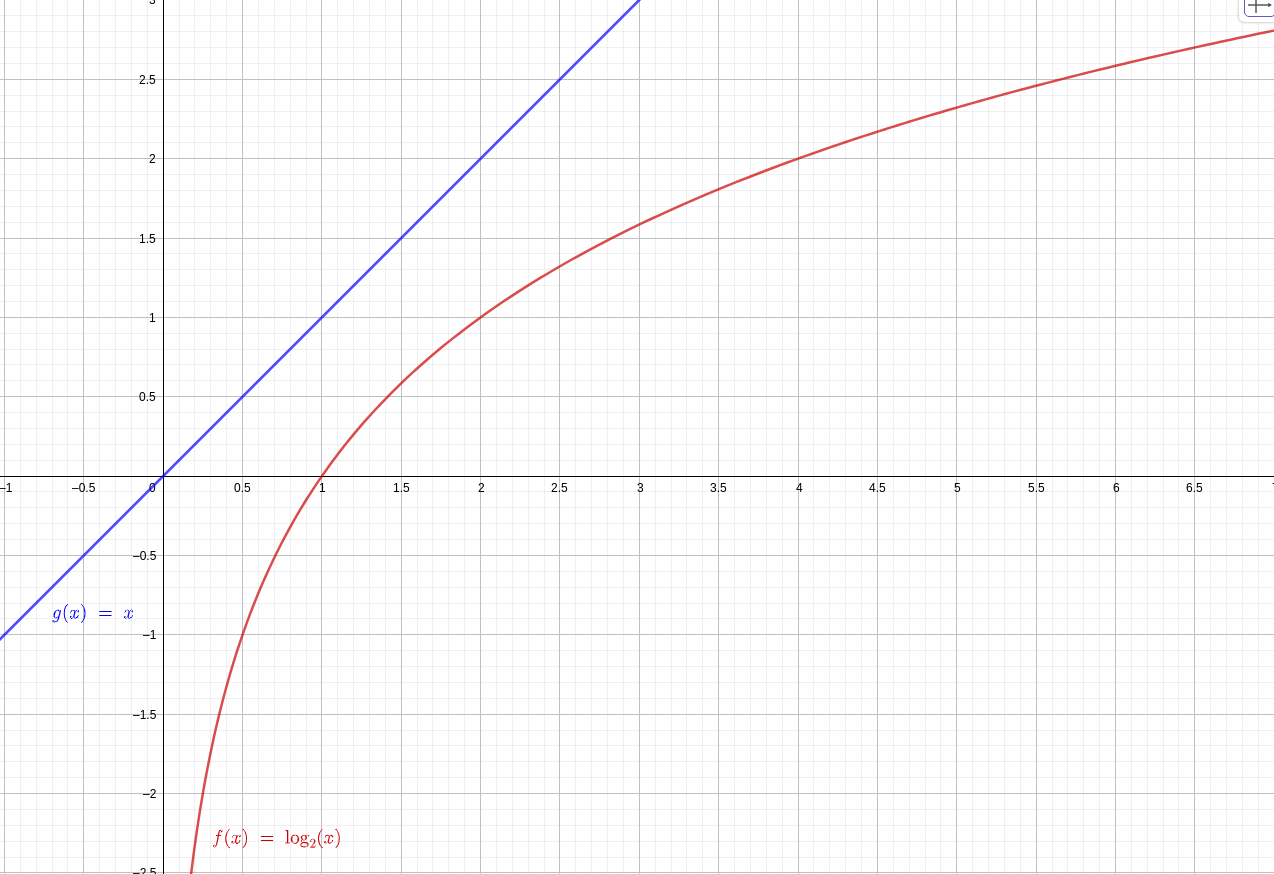
\includegraphics[scale=.2]{res/log_linear}
	\captionof{figure}{}\label{fig:log_linear}
\end{center}
Pertanto è possibile pensare di minorare la relazione sostituendo $n$ al termine sottrattivo presente ottenendo così una funzione più piccola\footnote{Sottraendo un qualcosa di più grande si ottiene l'effetto desiderato.}:
\begin{align*}
	c_{1} n \log_{2} n & \leq 2n \log_{2} + n -n = 2n \log_{2} < 2n \log_{2} n + n - \log_{2} n & \text{\textcolor{gray}{Minorando}}\\
	c_{1} &\leq \frac{2n \log_{2} n}{n \log_{2}n} \\
	c_{1} &\leq \frac{2 \cancel{n \log_{2} n}}{\cancel{n \log_{2} n}}\\
	c_{1} &\leq 2
\end{align*}
E otteniamo quindi $c_{1} = 2$. Nel svolgere la seconda disequazione possiamo sfruttare il fatto che, per ogni $n \geq 4$ vale: $n + \log_{2} n \leq n \log_{2} n$. Allora è possibile eseguire la seguente maggiorazione:
\begin{align*}
	2n \log_{2} n + n - \log_{2} n &< 2n \log_{2} n + n + \log_{2} n \leq 2n \log_{2} n + n \log_{2} n = 3n \log_{2} n \leq c_{2} n \log_{2} n
\end{align*}
da cui si ottiene $c_{2} \geq 3$ e quindi $c_{3}=3$. \hfill \blacksquare

\begin{exsbox}
	Si dimostri, \textbf{esplicitando il procedimento seguito nella sua interezza}, la verità o la falsità della seguente affermazione: se $f(n) = \Theta(\sqrt{g(n)})$ e $g(n)= \Theta((k(n))^{4})$ allora:
	\begin{displaymath}
		f(n) = \Theta((k(n))^{2})
	\end{displaymath}
	In caso affermativo, trovare le costanti che assicurano la validità della relazione.
\end{exsbox}

% Chapter 7: Grafi
\chapter{Strutture dati ramificate: i grafi}
\section{Introduzione}
Nel Capitolo 4 abbiamo visto come le strutture dati ramificate siano utili per rappresentare dati che hanno una struttura gerarchica. In questo capitolo vedremo come le strutture dati ramificate possono essere utilizzate per rappresentare dati che hanno una struttura non gerarchica, come ad esempio i grafi.

I grafi sono strutture dati che permettono di rappresentare relazioni tra entità. Per esempio, un grafo può essere utilizzato per rappresentare una rete di computer, dove i computer sono le entità e le connessioni tra i computer sono le relazioni. Un altro esempio è quello di un grafo che rappresenta una mappa stradale, dove i nodi sono le città e gli archi sono le strade che collegano le città. Per questo motivo, i grafi sono estremamente utili per risolvere problemi di ottimizzazione e di ricerca.
\section{Definizioni}
\dfn{Grafo}{
    Un \textbf{grafo} $G$ è una coppia ordinata $(V, E)$ dove $V$ è un insieme finito di elementi detti \textbf{nodi} e $E$ è un insieme di coppie di elementi di $V$ detti \textbf{archi}.
}

Come anticipato, i grafi sono estremamente utili per la rappresentazione di relazioni binarie all'interno di un insieme di elementi. L'insieme degli archi, $E$, può essere infatti visto come una relazione binaria su $V$: se $(u, v) \in E$, allora $u$ e $v$ sono collegati da un arco:
\begin{equation}
    E = \{(u, v) \in V \times V : u \text{ è collegato a } v\} \subseteq V \times V
\end{equation}
In particolare, se $E$ rappresenta una relazione binaria simmetrica\footnote{Una relazione binaria $\rho$ in un insieme $S$ si dice simmetrica se e solo se, per ogni $x,y \in S$ si ha $x \rho y \iff y \rho x$, ovvero $(x,y) \in G \iff (y,x) \in G$, dove $G$ è il grafico della relazione $\rho$.}, allora il grafo è detto \textbf{non orientato}. Altrimenti, se $E$ rappresenta una relazione binaria asimmetrica, allora il grafo è detto \textbf{orientato} e gli archi verranno rappresentati con delle frecce.


\begin{example}
	    Il grafo $G = (V, E)$ in Figura~\ref{fig:graph_1} è un grafo non orientato, dove \[V = \{A, B, C, D, E, F\}\] ed
	\begin{displaymath}
		E = \left\lbrace \begin{array}{llllllll}
			(A, D), & (D,A), & (A, E), &(E,A), & (B, E), & (E,B), & (B, F), &(F,B) \\
			(C, E),&(E,C), & (C, F),&(F,C), &(D, E),&(E,D), &(E, F), &(F,E)
		\end{array} \right\rbrace
	\end{displaymath}
    Il grafo $G_{2} = (V, E)$ in Figura~\ref{fig:graph_2} è un grafo orientato, dove \[V = \{A, B, C, D, E, F\}\] e \[E = \{(A, D), (A, E), (B, E), (B, F), (C, E), (C, F), (D, E), (E, F)\}\]
\end{example}

\begin{figure}[ht!]
\centering
\subfloat[Grafo non orientato\label{fig:graph_1}]{
\begin{tikzpicture}
	[node/.style={circle,draw,fill=blue!25!white,minimum size=0.5cm},>=latex]
    \node[node] (A) at (0,0) {A};
    \node[node] (B) at (2,0) {B};
    \node[node] (C) at (4,0) {C};
    \node[node] (D) at (0,2) {D};
    \node[node] (E) at (2,2) {E};
    \node[node] (F) at (4,2) {F};
    \draw [thick] (A) -- (D);
    \draw [thick] (A) -- (E);
    \draw [thick] (B) -- (E);
    \draw [thick] (B) -- (F);
    \draw [thick] (C) -- (E);
    \draw [thick] (C) -- (F);
    \draw [thick] (D) -- (E);
    \draw [thick] (E) -- (F);
\end{tikzpicture}}\hfil
\subfloat[Grafo orientato\label{fig:graph_2}]{
\begin{tikzpicture}
	[node/.style={circle,draw,fill=blue!25!white,minimum size=0.5cm},>=latex]
    \node[node] (A) at (0,0) {A};
    \node[node] (B) at (2,0) {B};
    \node[node] (C) at (4,0) {C};
    \node[node] (D) at (0,2) {D};
    \node[node] (E) at (2,2) {E};
    \node[node] (F) at (4,2) {F};
    \draw [thick,->] (A) -- (D);
    \draw [thick,->] (A) -- (E);
    \draw [thick,->] (B) -- (E);
    \draw [thick,->] (B) -- (F);
    \draw [thick,->] (C) -- (E);
    \draw [thick,->] (C) -- (F);
    \draw [thick,->] (D) -- (E);
    \draw [thick,->] (E) -- (F);
\end{tikzpicture}}
\caption{}
\end{figure}


\begin{osservation}
	    Sia $G=(V,E)$ un grafo, chiaramente il numero massimo di archi possibili sarà: \[|E| \leq |V| \times |V| = |V|^2\] Inoltre, se il grafo è non orientato, allora \[|E| \leq \frac{|V| \times (|V| - 1)}{2} = \binom{|V|}{2}\] Infatti, se il grafo è non orientato, allora: \[(u, v) \in E \iff (v, u) \in E\]
\end{osservation}

Molte definizioni per i grafi orientati e non orientati sono simili, sebbene alcuni termini abbiano significati leggermente diversi nei due contesti.

\dfn{Archi entranti, uscenti ed incidenti}{
    Se $(u,v)$ è un arco in un grafo orientato $G=(V,E)$, diciamo che $(u,v)$ \textbf{esce} dal vertice $u$ ed \textbf{entra} nel vertice $v$. Se $(u,v)$ è un arco in un grafo non orientato, diciamo che $(u,v)$ è \textbf{incidente} nei vertici $u$ e $v$.
}

\begin{figure}[ht!]
\centering
\subfloat[Grafo orientato\label{fig:graph_3}]{
\begin{tikzpicture}
	[node/.style={circle,draw,fill=blue!25!white,minimum size=0.5cm},>=latex]
    \node[node] (A) at (0,0) {4};
    \node[node] (B) at (2,0) {5};
    \node[node] (C) at (3,0) {6};
    \node[node] (D) at (0,2) {1};
    \node[node] (E) at (2,2) {2};
    \node[node] (F) at (3,2) {3};

    \draw[thick,->] (D) -- (E);
    \draw[thick,->] (E) -- (B);
    \draw[thick,->] (E) -- (A);
    \draw[thick,->] (A) -- (D);
    \draw[thick,->] (A) to [bend left = 15] (B);
    \draw[thick,->] (B) to [bend left = 15] (A);
    \draw[thick,->] (C) -- (F);
    \draw[thick,->] (E) to [out=330,in=300,looseness=8] (E);

\end{tikzpicture}
} \hfil
\subfloat[Grafo non orientato\label{fig:graph_4}]{
\begin{tikzpicture}
	[node/.style={circle,draw,fill=blue!25!white,minimum size=0.5cm}]
    \node[node] (A) at (0,0) {4};
    \node[node] (B) at (2,0) {5};
    \node[node] (C) at (3,0) {6};
    \node[node] (D) at (0,2) {1};
    \node[node] (E) at (2,2) {2};
    \node[node] (F) at (3,2) {3};

    \draw[thick] (D) -- (E);
    \draw[thick] (E) -- (B);
    \draw[thick] (B) -- (D);
    \draw[thick] (F) -- (C);

\end{tikzpicture}}
\caption{}
\end{figure}


\begin{osservation}
	    In Figura~\ref{fig:graph_3} il vertice $2$ ha due archi entranti e tre archi uscenti. In particolare, un arco che esce ed entra nello stesso vertice viene chiamato \textbf{cappio}. In Figura~\ref{fig:graph_4} il vertice $2$ ha due archi incidenti: $(1,2)$ e $(2,5)$. In un grafo non orientato non è possibile avere cappi.
\end{osservation}

\dfn{Relazione di adiacenza}{
	Se $(u,v)$ è un arco di un grafo $G=(V,E)$, diciamo che il vertice $v$ è \textbf{adiacente} al vertice $u$.
}

Se il grafo non è orientato, la relazione di adiacenza è simmetrica. Se il grafo è orientato, la relazione di adiacenza non è necessariamente simmetrica.


\begin{osservation}
		In Figura~\ref{fig:graph_3} e \ref{fig:graph_4} il vertice $2$ è adiacente al vertice 1, perché l'arco $(1,2)$ appartiene ad entrambi i grafi. Il vertice $1$ non è adiacente al vertice 2 nel grafo mostrato nella Figura~\ref{fig:graph_3} perché l'arco $(2,1)$ non appartiene al grafo.
\end{osservation}

\dfn{Grado di un vertice}{
	Il \textbf{grado} di un vertice in un grafo non orientato è il numero di archi che incidono nel vertice. Un vertice il cui grado è 0 si dice \textbf{isolato}. In un grafo orientato, il \textbf{grado uscente} di un vertice è il numero di archi che escono dal vertice; il \textbf{grado entrante} di un vertice è il numero di archi che entrano nel vertice. Il \textbf{grado} di un vertice in un grafo orientato è la somma del suo grado entrante e del suo grado uscente.
}


\begin{osservation}
		Il vertice 2 nella Figura \ref{fig:graph_4} ha grado 2 mentre il vertice 4 è isolato. Nel grafo in Figura \ref{fig:graph_3} il vertice 2 ha grado entrante 2, grado uscente 3 e grado 5.
\end{osservation}

\subsection{Percorsi in un grafo}\label{sez:grafi_def}

\dfn{Percorso in un grafo}{
	Un \textbf{percorso} di \textbf{lunghezza} $k$ da un vertice $u$ ad un vertice $u'$ in un grafo $G = (V,E)$ è una sequenza di vertici $\langle v_{0},v_{1}, \ldots, v_{k}\rangle$ tali che \[\begin{array}{l}
		u=v_{0} \\  u'=v_{k}
	\end{array}\] e \[\forall i=1,2,\ldots,k \qquad (v_{i-1},v_{i})\in E\]
	La  \textbf{lunghezza} del percorso, o \textbf{cammino}, è il numero di archi presenti nel cammino. Il cammino \textbf{contiene} i vertici $v_{0},v_{1}, \ldots, v_{k}$ e gli archi $(v_{0},v_{1}), (v_{1},v_{2}),\ldots,(v_{k-1},v_{k})$ (c'è sempre un cammino di lunghezza 0 da $u$ ad $u$). Se c'è un cammino $p$ da $u$ ad $u'$, diciamo che $u'$ è \textbf{raggiungibile} da $u$ attraverso $p$ e si denota con il simbolo $u' \leadsto u$. Un cammino si dice \textbf{semplice} se tutti i vertici nel cammino sono distinti.
}


\begin{osservation}
		Nella Figura~\ref{fig:graph_3}, il cammino $\langle 1,2,5,4 \rangle$ è un cammino semplice di lunghezza 3. Il cammino $\langle 2,5,4,5 \rangle$ invece non è semplice.
\end{osservation}

\dfn{Sottopercorso in un grafo}{
	Un \textbf{sottopercorso} di un percorso $p = \langle v_{0},v_{1},\ldots,v_{k}\rangle$ è una sottosequenza contigua dei suoi vertici. Ovvero, per ogni $0 \leq i \leq j \leq k$, la sottosequenza dei vertici $\langle v_{i},v_{i+1},\ldots,v_{k} \rangle$ è un sottopercorso di $p$.
}


\begin{osservation}
		Se la lunghezza di un percorso semplice è limitata dal numero di vertici presenti in un grafo, ovvero $|V|$, il numero di percorsi semplici in un grafo sarà anch'esso limitato in quanto queste saranno tutte e sole le sequenze di lunghezza minore od uguale della cardinalità di $V$.
\end{osservation}

\dfn{Ciclo}{
	In un grafo orientato un cammino $\langle v_{0},v_{1},\ldots,v_{k} \rangle$ forma un \textbf{ciclo} se $v_{0}=v_{k}$ e il cammino contiene almeno un arco. Il ciclo è \textbf{semplice} se $v_{1},...,v_{k}$ sono anche distinti. Un cappio è un ciclo di lunghezza 1. Un grafo orientato senza cappi si dice \textbf{semplice}. In un grafo non orientato un cammino $\langle v_{0},v_{1},\ldots,v_{k} \rangle$ forma un \textbf{ciclo (semplice)} se $k\geq 3,\; v_{0}=v_{k}$ e $v_{1},\ldots,v_{k}$ sono distinti. Un grafo senza cicli è detto \textbf{aciclico}.
}

\begin{figure}[ht!]
	\centering
	\subfloat[Grafo non connesso]{
		\begin{tikzpicture}
			[node/.style={circle,draw,fill=blue!25!white,minimum size=0.5cm}]
			\node[node] (A) at (0,1) {A};
			\node[node] (B) at (1,2) {B};
			\node[node] (C) at (2,2) {C};
			\node[node] (D) at (1,1) {D};
			\node[node] (E) at (2,1) {E};
			\node[node] (F) at (3,1) {F};

			\draw[thick] (A) -- (B);
			\draw[thick] (A) -- (D);
			\draw[thick] (B) -- (C);
			\draw[thick] (C) -- (D);
			\draw[thick] (C) -- (E);
		\end{tikzpicture}
	} \hfil
	\subfloat[Grafo connesso]{
		\begin{tikzpicture}
			[node/.style={circle,draw,fill=blue!25!white,minimum size=0.5cm}]

			\node[node] (A) at (0,1) {A};
			\node[node] (B) at (1,2) {B};
			\node[node] (C) at (2,2) {C};
			\node[node] (D) at (1,1) {D};
			\node[node] (E) at (2,1) {E};
			\node[node] (F) at (3,1) {F};

			\draw[thick] (A) -- (B);
			\draw[thick] (A) -- (D);
			\draw[thick] (B) -- (C);
			\draw[thick] (C) -- (D);
			\draw[thick] (C) -- (E);
			\draw[thick] (E) -- (F);
		\end{tikzpicture}
	}
	\caption{}
\end{figure}

Alcuni tipi di grafi hanno dei nomi speciali. Un \textbf{grafo completo} è un grafo non orientato in cui ogni coppia di vertici è adiacente. Un grafo aciclico e non orientato è una \textbf{foresta}; un grafo connesso, aciclico e non orientato è detto \textbf{albero libero}.


\begin{osservation}
		Gli alberi binari studiati nel capitolo 3 non sono altro che particolari tipi di grafi connessi, aciclici e non orientati in cui uno dei vertici si distingue da tutti gli altri, la radice, ed ogni vertice ha un grado entrante pari ad uno ed un grado uscente pari al massimo di due.
\end{osservation}

\section{Rappresentazione dei grafi}
Ci sono due metodi standard per la rappresentazione di un grafo $G=(V,E)$:
\begin{enumerate}
	\item come una collezione di \textbf{liste di adiacenza};
	\item come una \textbf{matrice di adiacenza}.
\end{enumerate}

Entrambi i metodi possono essere applicati sia ai grafi orientati che a quelli non orientati. Di solito, si preferisce la rappresentazione con liste di adiacenza, perché permette di rappresentare in modo compatto i grafi sparsi e richiede una minore occupazione di memoria al variare dei vertici del grafo.\footnote{Una matrice richiederebbe un costo spaziale quadratico sul numero di vertici ($|V|^{2}$) mentre la rappresentazione attraverso liste di adiacenza solo un costo lineare ($|V|$).}

\subsection{Le liste di adiacenza}
La \textbf{rappresentazione con liste di adiacenza} di un grafo $G=(V,E)$ consiste in un array $Adj$ di $|V|$ liste, una per ogni vertice in $V$. Per ogni $u \in V$, la lista di adiacenza $Adj[u]$ contiene tutti i vertici $v$ tali che esista un arco $(u,v)\in E$. Ovvero $Adj[u]$ include tutti i vertici \textbf{adiacenti} ad $u$ in $G$.

Le liste di adiacenza (vedi Figura \ref{fig:lista_adiacenza}) possono essere facilmente adattate per rappresentare i \textbf{grafi pesati}, cioè i grafi per i quali ogni arco ha un \textbf{peso} associato. In questi casi, il peso $w(u,v)$ dell'arco $(u,v) \in E$ viene memorizzato semplicemente assieme al vertice $v$ nella lista di adiacenza di $u$.

\subsection{Le matrici di adiacenza}
Uno svantaggio potenziale della rappresentazione con liste di adiacenza è che non c'è modo più veloce per determinare se un particolare arco $(u,v)$ è presente nel grafo invece che scorrere la lista $Adj[u]$. Per porre un rimedio a questo svantaggio, si può rappresentare il grafo con una \textbf{matrice di adiacenza}, al costo di usare una maggiore quantità di memoria.

Per la \textbf{rappresentazione con matrice di adiacenza} (vedi Figura \ref{fig:matrice_adiacenza}) di un grafo $G=(V,E)$ si suppone che i vertici siano numerati $1,2,\ldots,|V|$ in modo arbitrario. La rappresentazione con matrice di adiacenza di un grafo $G$ consiste in una matrice $A=(a_{ij})$ di dimensioni $|V| \times |V|$ che descrive la \textbf{funzione caratteristica} in $E$:
\begin{equation}
	a_{ij} = \begin{cases}
		1 & \text{se } (i,j)\in E \\
		0 & \text{altrimenti}
	\end{cases}
\end{equation}

\begin{figure}[ht!]
	\centering
	\subfloat[\label{fig:grafo}]
	{
	\begin{tikzpicture}
		[node/.style={circle,draw,fill=blue!25!white,minimum size=0.5cm}]
		\node[node,name=1] at (0,1) {1};
		\node[node,name=2] at (1,1) {2};
		\node[node,name=3] at (2,0.5) {3};
		\node[node,name=5] at (0,0) {5};
		\node[node,name=4] at (1,0) {4};
		\draw[thick] (1)--(2);
		\draw[thick] (1)--(5);
		\draw[thick] (2)--(3);
		\draw[thick] (2)--(4);
		\draw[thick] (2)--(5);
		\draw[thick] (3)--(4);
		\draw[thick] (5)--(4);
	\end{tikzpicture}
	} \hfil
	\subfloat[\label{fig:lista_adiacenza}]
	{
	\begin{tikzpicture}
		% draw adjacency list of previous graph
		\node[draw,rectangle,minimum size=0.5cm,fill=blue!25] (1) at (0,1) {};
		\node[draw,rectangle,minimum size=0.5cm,fill=blue!25] (2) at (0,0.5) {};
		\node[draw,rectangle,minimum size=0.5cm,fill=blue!25] (3) at (0,0) {};
		\node[draw,rectangle,minimum size=0.5cm,fill=blue!25] (4) at (0,-0.5) {};
		\node[draw,rectangle,minimum size=0.5cm,fill=blue!25] (5) at (0,-1) {};
		\node[left] at (1.west) {1};
		\node[left] at (2.west) {2};
		\node[left] at (3.west) {3};
		\node[left] at (4.west) {4};
		\node[left] at (5.west) {5};

		\node[draw,rectangle,minimum size=0.5cm,fill=blue!25] (12) at (1,1) {2};
		\node[draw,rectangle,minimum size=0.5cm,fill=blue!25] (121) at (1.5,1) {};
		\node[draw,rectangle,minimum size=0.5cm,fill=blue!25] (15) at (2.5,1) {5};
		\node[draw,rectangle,minimum size=0.5cm,fill=blue!25] (151) at (3,1) {nil};
		\draw[thick,->] (1) -- (12);
		\draw[thick,->] (121) -- (15);

		\node[draw,rectangle,minimum size=0.5cm,fill=blue!25] (21) at (1,0.5) {1};
		\node[draw,rectangle,minimum size=0.5cm,fill=blue!25] (212) at (1.5,0.5) {};
		\node[draw,rectangle,minimum size=0.5cm,fill=blue!25] (22) at (2.5,0.5) {5};
		\node[draw,rectangle,minimum size=0.5cm,fill=blue!25] (221) at (3,0.5) {};
		\node[draw,rectangle,minimum size=0.5cm,fill=blue!25] (23) at (4,0.5) {3};
		\node[draw,rectangle,minimum size=0.5cm,fill=blue!25] (231) at (4.5,0.5) {};
		\node[draw,rectangle,minimum size=0.5cm,fill=blue!25] (24) at (5.5,0.5) {4};
		\node[draw,rectangle,minimum size=0.5cm,fill=blue!25] (241) at (6,0.5) {nil};
		\draw[thick,->] (2) -- (21);
		\draw[thick,->] (212) -- (22);
		\draw[thick,->] (221) -- (23);
		\draw[thick,->] (231) -- (24);

		\node[draw,rectangle,minimum size=0.5cm,fill=blue!25] (31) at (1,0) {2};
		\node[draw,rectangle,minimum size=0.5cm,fill=blue!25] (311) at (1.5,0) {};
		\node[draw,rectangle,minimum size=0.5cm,fill=blue!25] (32) at (2.5,0) {4};
		\node[draw,rectangle,minimum size=0.5cm,fill=blue!25] (321) at (3,0) {nil};
		\draw[thick,->] (3) -- (31);
		\draw[thick,->] (311) -- (32);

		\node[draw,rectangle,minimum size=0.5cm,fill=blue!25] (41) at (1,-0.5) {2};
		\node[draw,rectangle,minimum size=0.5cm,fill=blue!25] (411) at (1.5,-0.5) {};
		\node[draw,rectangle,minimum size=0.5cm,fill=blue!25] (42) at (2.5,-0.5) {5};
		\node[draw,rectangle,minimum size=0.5cm,fill=blue!25] (421) at (3,-0.5) {};
		\node[draw,rectangle,minimum size=0.5cm,fill=blue!25] (43) at (4,-0.5) {3};
		\node[draw,rectangle,minimum size=0.5cm,fill=blue!25] (431) at (4.5,-0.5) {nil};
		\draw[thick,->] (4) -- (41);
		\draw[thick,->] (411) -- (42);
		\draw[thick,->] (421) -- (43);

		\node[draw,rectangle,minimum size=0.5cm,fill=blue!25] (51) at (1,-1) {4};
		\node[draw,rectangle,minimum size=0.5cm,fill=blue!25] (511) at (1.5,-1) {};
		\node[draw,rectangle,minimum size=0.5cm,fill=blue!25] (52) at (2.5,-1) {1};
		\node[draw,rectangle,minimum size=0.5cm,fill=blue!25] (521) at (3,-1) {};
		\node[draw,rectangle,minimum size=0.5cm,fill=blue!25] (53) at (4,-1) {2};
		\node[draw,rectangle,minimum size=0.5cm,fill=blue!25] (531) at (4.5,-1) {nil};
		\draw[thick,->] (5) -- (51);
		\draw[thick,->] (511) -- (52);
		\draw[thick,->] (521) -- (53);
	\end{tikzpicture}
	} \hfil
	\subfloat[\label{fig:matrice_adiacenza}]
	{
	\begin{tikzpicture}[every node/.style=draw]
	\pgfmatrix{rectangle}{center}{mymatrix}
	{\pgfusepath{}}{\pgfpointorigin}{\let\&=\pgfmatrixnextcell}
	{
		\node (a){0}; \& \node(b) {1}; \& \node (c) {0}; \& \node (d) {0}; \& \node (e) {1}; \\
		\node (f){1}; \& \node(g) {0}; \& \node (h) {1}; \& \node (i) {1}; \& \node (l) {1}; \\
		\node (m){0}; \& \node(n) {1}; \& \node (o) {0}; \& \node (p) {1}; \& \node (q) {0}; \\
		\node (r){0}; \& \node(s) {1}; \& \node (t) {1}; \& \node (u) {0}; \& \node (v) {1}; \\
		\node (w){1}; \& \node(x) {1}; \& \node (y) {0}; \& \node (z) {1}; \& \node (aa) {0}; \\
	}
	\node[left,draw=white] at (a.west) {1};
	\node[left,draw=white] at (f.west) {2};
	\node[left,draw=white] at (m.west) {3};
	\node[left,draw=white] at (r.west) {4};
	\node[left,draw=white] at (w.west) {5};
	\node[above,draw=white] at (a.north) {1};
	\node[above,draw=white] at (b.north) {2};
	\node[above,draw=white] at (c.north) {3};
	\node[above,draw=white] at (d.north) {4};
	\node[above,draw=white] at (e.north) {5};
	\end{tikzpicture}
	}
	\caption{Due rappresentazioni di un grafo non orientato. \textbf{(\ref{fig:grafo})} Un grafo non orientato $G$ con cinque vertici e sette archi. \textbf{(\ref{fig:lista_adiacenza})} Una rappresentazione con liste di adiacenza di $G$. \textbf{(\ref{fig:matrice_adiacenza})} Una rappresentazione con matrice di adiacenza di $G$.}
\end{figure}

\section{Visita in ampiezza}
La \textbf{visita in ampiezza} (\textsc{Breadth-First-Search}) è uno dei più semplici algoritmi di ricerca nei grafi e sta alla base di molti algoritmi che operano con i grafi. Dato un grafo $G=(V,E)$ e un vertice distinto $s$, detto \textbf{sorgente}, la visita in ampiezza ispeziona sistematicamente gli archi di $G$ per ``scoprire'' tutti i vertici raggiungibili da $s$ individuando la distanza da $s$ ad ognuno dei vertici raggiungibili. La visita in ampiezza è chiamata così infatti perché espande la frontiera fra i vertici scoperti e quelli da scoprire in maniera uniforme lungo l'ampiezza della frontiera. Questo significa che l'algoritmo scopre tutti i vertici che si trovano ad una distanza $k$ da $s$, prima di scoprire i vertici a distanza $k+1$.

Per tenere traccia del lavoro svolto ed evitare di raggiungere nodi già visitati in precedenza, la visita in ampiezza colora i vertici di bianco, di grigio o di nero:
\begin{itemize}
	\item \textbf{Bianco:} il nodo non è stato ancora visitato;
	\item \textbf{Grigio:} il nodo è stato visitato ma potrebbe avere di vicini non visitati;
	\item \textbf{Nero:} il nodo è stato visitato ed anche tutti i suoi vicini.
\end{itemize}
Inizialmente tutti i vertici sono bianchi; successivamente possono diventare grigi ed infine neri. Per questo motivo possiamo implementare l'algoritmo \textsc{Init(G)} (Algoritmo~\ref{lst:init}) che si occupa di inizializzare un grafo colorando tutti i suoi vertici di bianco.
\begin{lstlisting}[language=asd,caption={Init(G)},label=lst:init]
for each v in V do
	Color[v] = White
\end{lstlisting}

Un vertice viene \textbf{scoperto} quando viene incontrato per la prima volta durante la visita; in quel momento cessa di essere un vertice bianco. Se $(u,v) \in E$ e il vertice $u$ è nero, allora il vertice $v$ è grigio oppure nero: ovvero tutti i vertici adiacenti ai vertici neri sono sempre scoperti. I vertici grigi possono avere qualche vertice bianco adiacente per questo motivo essi rappresentano la frontiera fra i vertici scoperti e quelli da scoprire.

\begin{center}
	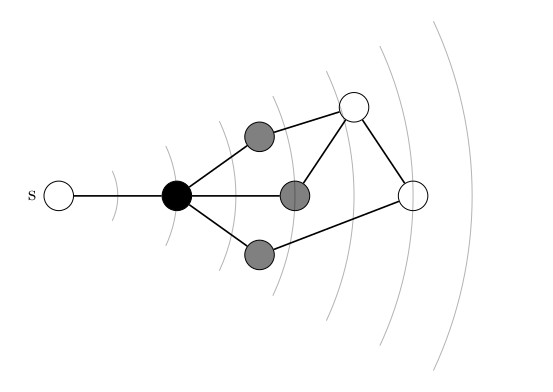
\includegraphics{res/dfs_frontiera}
	\captionof{figure}{L'algoritmo di visita in ampiezza estende di volta in volta la frontiera dei vertici da visitare}
\end{center}

La vista in ampiezza costruisce una coda $Q$ che, inizialmente contiene soltanto il vertice sorgente $s$. A questo punto si accodano tutti i vertici presenti colorati di bianco scoperti esplorando la lista di adiacenza e li si colora di grigio. Una volta aver eseguito questa operazione si estrae il nodo in testa alla coda, lo si colora di nero e si aggiungono in coda i  vertici bianchi adiacenti scoperti esplorando la lista di adiacenza. L'algoritmo viene eseguito fino a quando la coda non risulta vuota.


\begin{lstlisting}[language=asd,caption={BFS(G,s)},label=lst:bfs_graph]
Init(G)
Q={s}
Color[s] = Gray
while Q @\neq@ {} do
	x = Head(Q)
	foreach v @\in@ Adj(x) do
		if Color[v] = b then
			Q = Enqueue(Q,v)
			Color[v] = Gray
	Q = Dequeue(Q)
	Color[x] = Black
\end{lstlisting}

\subsection{Una versione migliorata dell'algoritmo BFS}
L'Algoritmo~\ref{lst:bfs_graph} visita i vertici raggiungibili di un grafo al crescere della loro distanza dal vertice sorgente $s$. Ciò significa che ciascun vertice viene raggiunto tramite il cammino più breve possibile da $s$. Infatti, per ogni vertice $v$ raggiungibile da $s$, il cammino semplice che va da $s$ a $v$ corrisponde ad un cammino minimo da $s$ a $v$, cioè un cammino che contiene il minor numero di archi possibile.

\dfn{Distanza di un vertice}{
	La \textbf{distanza} di un vertice $v$ dal vertice sorgente $s$ è il numero di archi nel cammino minimo da $s$ a $v$, e si indica con $d(s,v)$.
}

Osserviamo che l'algoritmo \textsc{BFS} determina una \textit{relazione gerarchica} fra i vertici di un grafo. Infatti, la visita in ampiezza costruisce un albero, detto \textbf{albero breath first (BF)}, che inizialmente contiene soltanto la sua radice, ovvero il vertice sorgente $s$. Quando un vertice bianco $v$ viene scoperto durante l'ispezione della lista di adiacenza di un vertice $u$ già scoperto, il vertice $v$ e l'arco $(u,v)$ vengono aggiunti all'albero. Il vertice $u$ rappresenta così il \textbf{predecessore} o \textbf{padre} di $v$ nell'albero \textsc{BF} e dato che un vertice verrà scoperto sempre e solo una volta, ogni vertice avrà sempre e solo un padre nell'albero \textsc{BF}. È così univocamente determinata la funzione $$p:V \rightarrow \mathbb{N}\cup \{nil\}$$ che associa ad ogni nodo l'indice del vertice padre. A partire da questa osservazione possiamo definire un raffinamento dell'Algoritmo~\ref{lst:bfs_graph} che costruisce l'albero \textsc{BF} a partire dai percorsi minimi da $s$ a tutti i vertici raggiungibili.

L'Algoritmo~\ref{lst:bfs_graph_2} calcola quindi la distanza di ogni vertice raggiungibile da $s$ come il numero di archi nel cammino minimo da $s$ al vertice. Questa quantità è memorizzata nell'array $d$. Chiaramente, la distanza da $s$ a $v$ è data dalla distanza da $s$ al suo predecessore, più 1. Useremo il valore $\infty$ per indicare che un vertice non è raggiungibile da $s$. Oltre al vettore $d$ che memorizza le distanze, l'algoritmo utilizza un vettore $p$ che memorizza i predecessori di ogni vertice nell'albero \textsc{BF}. Il predecessore di un vertice $v$ è il vertice $u$ che ha scoperto $v$ per la prima volta. Il predecessore di $s$ è indicato con il valore $nil$.

\begin{lstlisting}[language=asd,caption={BFS(G,s)},label=lst:bfs_graph_2]
for each x in V do
	Color[x] = white
	d[x]=@$\infty$@
	p[x] = nil
Q={s}
Color[s] = Gray
d[s] = 0
p[s] = nil
while Q @\neq@ {} do
	x = Head(Q)
	foreach v @\in@ Adj(x) do
		if Color[v] = b then
			Q = Enqueue(Q,v)
			Color[v] = Gray
			d[v] = d[x] + 1
			p[v] = x
	Q = Dequeue(Q)
	Color[x] = Black
\end{lstlisting}

\subsection{Correttezza dell'algoritmo BFS}
Prima di dimostrare le varie proprietà della visita in ampiezza, analizziamo il suo tempo di esecuzione con un grafo di input $G=(V,E)$.

Dopo l'inizializzazione, nessun vertice sarà più colorato di bianco, quindi il test nella riga 12 garantisce che ciascun vertice venga accodato al più una volta, e di conseguenza, venga eliminato dalla coda al più una volta. Le operazioni di inserimento e cancellazione dalla coda richiedono un tempo costante, quindi il tempo totale dedicato alle operazioni con la coda risulta lineare sulla dimensione dei vertici del grafo $G$.

Poiché la lista di adiacenza di ciascun vertice viene ispezionata soltanto quando il vertice viene rimosso dalla coda, ogni lista di adiacenza viene ispezionata al più una volta. Poiché l'algoritmo ispeziona le liste di adiacenza di ciascun vertice, la cui somma totale \footnote{Di tutte le liste.}delle lunghezze è pari ad $|E|$, allora il tempo di esecuzione totale di \textsc{BFS} risulta lineare nella dimensione della rappresentazione con liste di adiacenza del grafo $G$: $E+V$.


\begin{teorbox}
	Dato un arbitrario grafo $G$ ed un vertice $s \in V$, al termine dell'esecuzione dell'Algoritmo \textsc{BFS} devono valere:
\begin{enumerate}
	\item $\forall v \in V$, $v$ sarà visitato se e soltato se $v$ è \textit{raggiungibile} da $s$;
	\item $\forall v \in V$ vale: $d[v] = \delta(v,s)$;
	\item $\forall v \in V\setminus\{s\}$, se $v$ è raggiungibile allora è ottenibile un percorso minimo da $s$ a $v$ concatenando il percorso minimo da $s$ a $p[v]$.
\end{enumerate}
\end{teorbox}

Il teorema appena enunciato garantisce la correttezza dell'algoritmo \textsc{BFS}. Al contrario degli algoritmi finora visti, dove si è utilizzato il principio di induzione per dimostrare la correttezza, la dimostrazione della correttezza dell'algoritmo \textsc{BFS} non è così immediata in quanto l'algoritmo è stato definito in maniera iterativa. Per dimostrare quindi tale correttezza bisogna studiare il comportamento del programma durante l'esecuzione e dimostrare che le tre proprietà enunciate dal teorema sono sempre valide. Questa tipologia di analisi prende il nome di \textbf{analisi a invariante}.

\begin{propbox}[Proprietà della funzione $\delta$ o disuguaglianza triangolare]
Per ogni coppia $(u,v)$ di vertici di un grafo $G$, se $(u,v) \in E$ allora $\delta(s,v) \leq \delta(s,u) + 1$ per ogni vertice $s$.
\begin{center}
	\begin{tikzpicture}
		% draw a graph with three paths and describe the delta function's property
		[node/.style={circle,draw,fill=blue!25!white,minimum size=0.5cm},>=latex]
		\node[node] (u) at (0,0) {s};
		\node[node] (v) at (2,0) {u};
		\node[node] (w) at (1,-1) {v};

		\draw[thick] (u) -- (v);
		\draw[thick] (u) -- (w);
		\draw[thick] (w) -- (v);

		\node[above] at (1,0) {$\pi_{u}$};
		\node[below] at (0.5,-0.5) {$\pi_{v}$};
		\node[below] at (1.5,-0.5) {};

		\node[above] at (1,-1.5) {};
	\end{tikzpicture}
\end{center}
\end{propbox}

\begin{proof}
	Supponiamo che la proprietà sia falsa. Allora esiste una coppia $(u,v)$ di vertici di un grafo $G$ tale che $(u,v) \in E$ e $\delta(s,v) > \delta(s,u) + 1$ per ogni vertice $s$.

Sia $\pi_{u}$ un cammino minimo da $s$ a $u$ e sia $\pi_{v}$ un cammino minimo da $s$ a $v$ e consideriamo il percorso $\pi_{u} \cdot v$. Questo percorso è un cammino da $s$ a $v$ e la sua lunghezza è $\delta(s,u) + 1$. Poiché $\delta(s,v) > \delta(s,u) + 1$, allora $\pi_{u} \cdot v$ è un cammino da $s$ a $v$ più corto di $\pi_{v}$, il che è assurdo perché $\pi_{v}$ è un cammino minimo da $s$ a $v$.
\end{proof}


\begin{propbox}[Proprietà A]
	Durante l'esecuzione di \textsc{BFS}$(G,s)$, per ogni vertice $v \in V$ si ha:
	\begin{displaymath}
		d[v] \geq \delta(s,v)
	\end{displaymath}
\end{propbox}
\begin{proof}
	Per dimostrare l'invarianza della proprietà A si procede per induzione sul numero di accodamenti in $Q$. Questo perché le modifiche ai valori di $d[v]$ avvengono soltanto in corrispondenza degli accodamenti dei vertici in $Q$. Tutto ciò che non è un accodamento, infatti, non modifica i valori di $d[v]$. Indichiamo tale numero con $k$:
\begin{enumerate}
	\item \textbf{Caso base:} Sia $k=0$. All'inizio dell'esecuzione di \textsc{BFS}$(G,s)$, $Q$ contiene soltanto il vertice $s$. Poiché $d[s]=0$ e $\delta(s,s)=0$, la proprietà A è verificata.
	\item \textbf{Caso induttivo:} Sia $k>1$ e assumiamo che la proprietà sia verificata per $k-1$ accodamenti. Tra il $k-1$-esimo ed il $k$-esimo accodamento non avviene alcuna modifica ai valori di $d$. Sia $x$ l'ultimo vertice accodato e supponiamo di eseguire l'accodamento di un vertice $v$. Essendo $x$ già presente nella coda la sua distanza è stata già calcolata e vale, per ipotesi induttiva:
	\[d[x] \geq \delta(s,x)\]
	Maggiorando entrambi i membri della disuguaglianza triangolare con $+1$ si ottiene:
	\[d[x]+1 \geq \delta(s,x)+1\]
	Dovendo accodare $v$ si presuppone che esista un arco che vada da $x$ a $v$, ovvero $(x,v) \in E$. Per la proprietà della funzione $\delta$ si ha allora:
	\[\delta(s,x) + 1 \geq \delta(s,v) \]
	Per transitività si ottiene:
	\[d[x]+1 \geq \delta(s,v)\]
	Per la definizione di $d[v]$ si ha quindi l'enunciato:
	\[d[v] \geq \delta(s,v)\]
\end{enumerate}
\end{proof}

Una seconda proprietà invariante che andiamo a dimostrare descrive la relazione fra le stime delle distanze dei vertici accodati.

\begin{propbox}[Proprietà B]
	Durante l'esecuzione di \textsc{BFS}$(G,s)$, se $Q=\langle v_{1},v_{2},\ldots,v_{k}\rangle$ allora valgono le seguenti proprietà:
	\begin{enumerate}
		\item $d[v_{k}] \leq d[v_{1}]+1$;
		\item $d[v_{i}] \leq d[v_{i+1}]$ per $i=1,2,\ldots,k-1$.
	\end{enumerate}
\end{propbox}
\begin{proof}
	Come già osservato in precedenza, le stime delle distanze vengono modificate soltanto in corrispondenza delle operazioni eseguite sulla coda $Q$, per questo motivo bisogna tenere in considerazione tutte le operazioni di accodamento e decodamento. Sia $k$ il numero di tali operazioni e procediamo per induzione su $k$:
\begin{itemize}
	\item \textbf{Caso base:} Sia $k=0$. All'inizio dell'esecuzione di \textsc{BFS}$(G,s)$, $Q$ contiene soltanto il vertice $s$. Poiché $d[s]=0$ le due proprietà sono banalmente verificate.
	\item \textbf{Caso induttivo:} Sia $k>1$, bisogna dimostrare che la proprietà sia valida dopo l'inserimento e la rimozione di un vertice nella coda. Se il vertice $v_{1}$ viene eliminato dalla coda, il vertice $v_{2}$ diventa la nuova testa (se la coda si svuota, allora ci troviamo nuovamente nel caso base). Per l'ipotesi induttiva si ha:
	\[d[v_{1}] \leq d[v_{2}]\]
	ma allora si ha:
	\[d[v_{k}]\leq d[v_{1}]+1 \leq d[v_{2}]+1\]
	e le restanti disuguaglianze restano inalterate. L'inserimento di un nuovo vertice richiede invece un esame più attento del codice. Quando inseriamo nella coda un vertice $v$, questo diventa l'ultimo elemento della coda, ovvero $v_{k+1}$ e si pone:
	\[d[v_{k+1}] = d[x]+1\]
	dove $x$ rappresenta la testa della coda prima dell'inserimento di $v$,	il che dimostra la prima proprietà. Per la seconda proprietà bisogna dimostrare che:
	\[ d[v_{k}] \leq d[v_{k+1}] \]
	Chiaramente, prima dell'accodamento del vertice $v$ valeva la seguente relazione per vertice $v_{k}$:
	\[ d[v_{k}] \leq d[v_{1}]+1 = d[v_{k+1}] \]
	che è la tesi della seconda proprietà.
\end{itemize}
\end{proof}

\begin{propbox}[Proprietà C]
	È possibile partizionare l'insieme dei vertici $V$ in varie partizioni $V_{0},V_{1},\ldots,V_{k}$ tali che:
	\begin{itemize}
		\item $V_{0} = \{s\}$;
		\item $V_{1}$ contiene i vertici adiacenti di $s$ meno $s$ stesso;
		\item $V_{2}$ contiene i vertici adiacenti di $V_{i-1}$ meno i vertici già presenti in $V_{0},V_{1}$.
		\item $V_{i}$ contiene i vertici adiacenti di $V_{i-1}$ meno i vertici già presenti in $V_{0},V_{1},\ldots,V_{i-1}$.
		\item $V_{\infty}$ contiene i vertici non raggiungibili da $s$.
	\end{itemize}
\end{propbox}

Si osserva che un vertice non raggiungibile $v$ non può mai essere accodato. Infatti, se per assurdo si suppone che $v$ sia il primo vertice non raggiungibile ad essere accodato, allora deve esistere un vertice $x \in Q$ per cui $(x,v) \in E$. Essendo $x$ un vertice raggiungibile allora esiste sicuramente un percorso dalla sorgente al vertice $v$ che passa per $x$. Ma allora $v$ è raggiungibile, il che è assurdo. Quindi, se $v$ non è raggiungibile, allora $v$ non può essere accodato. Grazie a questa osservazione è possibile dimostrare la correttezza dell'algoritmo \textsc{BFS} semplicemente dimostrando il seguente lemma.

\begin{lemmabox}
	Per ogni $i \in \mathbb{N}$, per ogni vertice $v \in V_{i}$ vale che esiste un unico istante durante l'esecuzione dell'algoritmo \textsc{BFS} tale per cui:
	\begin{enumerate}
		\item $v$ viene colorato di grigio e aggiunto alla coda $Q$;
		\item $d[v] = i$;
		\item il predecessore di $v$ è impostato ad un vertice $u \in V_{i-1}$ e $(p[v],v) \in E$ con $v \neq s$.
	\end{enumerate}
\end{lemmabox}
\begin{proof}
	Si dimostra per induzione su $i$:
\begin{enumerate}
	\item \textbf{Caso base:} $i=0$ e $v=s$. All'inizio dell'esecuzione di \textsc{BFS}$(G,s)$, $Q$ contiene soltanto il vertice $s$ e le tre proprietà sono banalmente vere.
	\item \textbf{Caso induttivo:} sia $i>0$ e si supponga il lemma vero per $V_{j}$ con $j<i$. Se $v \in V_{i}$ arbitrario allora esiste per forza un momento in cui questo verrà colorato di grigio ed accodato. Ciò significa che esiste un percorso da $s$ a $v$ che passa per un vertice $x$ che è stato accodato al più $i-1$-esimo accodamento. Quindi, $x \in V_{i-1}$. Per ipotesi induttiva allora $d[x] = i-1$ e $p[x] \in V_{i-2}$. Poiché $x$ è stato accodato al più $i-1$-esimo accodamento, allora $v$ è stato accodato al $i$-esimo accodamento. Quindi, $d[v] = d[x]+1 = (i-1)+1 = i$ e $p[v] = x$.
\end{enumerate}
\end{proof}

\section{Visita in profondità}
A differenza della visita in ampiezza che si propone di visitare un grafo per distanze crescenti, la visita in profondità (\textsc{Depth-First-Search}) si propone di visitare un grafo esplorando tutti i nodi visitabili lungo i vari percorsi che si diramano a partire da un nodo sorgente $s$.

La visita in profondità è stata già descritta in relazione alle strutture dati ramificate come gli alberi dove, a differenza dei grafi, è implicita nella struttura il concetto di \textit{figlio sinistro} e \textit{figlio destro}. In un grafo, invece, non esiste alcuna relazione gerarchica tra i vari nodi e sarà quindi necessario adottare una strategia diversa da quella utilizzata per la visita in ampiezza che faceva uso di una coda per memorizzare i nodi da visitare.

Nella visita in profondità, ci avvaleremo di quattro array ausiliari per memorizzare lo stato dei nodi del grafo:
\begin{enumerate}
	\item \texttt{Color[]} che memorizza lo stato dei nodi codificati per colore: \texttt{White} se il nodo non è stato ancora visitato, \texttt{Gray} se il nodo è stato visitato ma non tutti i suoi vicini sono stati visitati, \texttt{Black} se il nodo è stato visitato e tutti i suoi vicini sono stati visitati;
	\item \texttt{d[]} che memorizza il tempo di scoperta di un nodo;
	\item \texttt{f[]} che memorizza il tempo di completamento di un nodo;
	\item \texttt{p[]} che memorizza il predecessore di un nodo.
\end{enumerate}
Per memorizzare i vari istanti di tempo assumiamo di dichiarare una variabile globale \texttt{time} che verrà incrementata ad ogni chiamata ricorsiva della funzione \textsc{DFS-Visit}. Si hanno quindi i seguenti algoritmi: \texttt{Init(G)}, \texttt{DFS(G)} e \texttt{DFS-Visit(G,u)}. L'algoritmo \texttt{Init(G)} inizializza gli array ausiliari \texttt{pred[]} e \texttt{color[]}, mentre l'algoritmo \texttt{DFS(G)} esegue la visita in profondità del grafo $G$ richiamando la funzione \texttt{DFS-Visit(G,u)} per ogni nodo $u \in V$ che non è ancora stato visitato.
\begin{center}
\begin{minipage}{,4\textwidth}
\begin{lstlisting}[language=asd,caption={Init(G)},label=lst:init_graph]
for each v @$\in$@ V do
	Color[v] = White
	Pred[v] = nil
time = 1
\end{lstlisting}
\end{minipage}
\begin{minipage}{0.4\textwidth}
	\begin{lstlisting}[language=asd,caption={DFS(G)},label=lst:dfs_graph]
	Init(G)
	for each v @$\in$@ V do
		if Color[v] = White then
			DFS-Visit(G,v)
	\end{lstlisting}
\end{minipage}
\end{center}
\begin{lstlisting}[language=asd,caption={DFS-Visit(G,s)},label=lst:dfs_visit_graph]
Color[s] = Gray
time = time+1
d[s] = time
for each v @$\in$@ Adj(s) do
	if Color[v] = White then
		Pred[v] = s
		DFS-Visit(G,v)
time = time+1
f[s] = time
Color[s] = Black
\end{lstlisting}

\begin{center}
	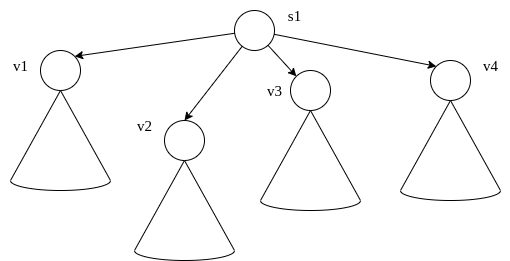
\includegraphics[scale=0.55]{res/DFS_forest}
	\captionof{figure}{Foresta generata dalla visita in profondità di un grafo.}\label{fig:fdf}
\end{center}

Come nella visita in ampiezza, quando un vertice $v$ viene scoperto durante un'ispezione della lista di adiacenza di un vertice $s$ già scoperto, la visita in profondità registra questo evento assegnando $pred[v]=s$. Diversamente dalla visita in ampiezza però, dove l'ispezione delle liste di adiacenza produceva un albero dei predecessori (l'albero BF), la visita in profondità genera una foresta di alberi, detta \textbf{foresta depth first (DF)} (vedi Figura \ref{fig:fdf}), che è composta da vari \textbf{alberi depth first (DF)} in quanto la visita può essere ripetuta da più sorgenti. L'albero DF di un vertice $s$ è composto da tutti i vertici raggiungibili da $s$ e da tutti gli archi $(s,v)$ tali che $v$ è il primo vertice scoperto durante la visita di $s$.

Volendo fare una analisi del tempo di esecuzione dell'algoritmo \textsc{DFS} si osserva che ciascuna chiamata ricorsiva della funzione \textsc{DFS-Visit} richiede un tempo costante per inizializzare il colore del vertice $u$ e un tempo lineare sulla dimensione della lista di adiacenza di $u$ per ispezionarla completamente. Poiché la somma delle lunghezze di tutte le liste di adiacenza è pari a $|E|$, il tempo totale richiesto per ispezionare tutte le liste di adiacenza è lineare su tale grandezza. Inoltre, poiché ogni vertice viene visitato una sola volta, si avrà che il numero totale di chiamate sia lineare sul numero dei vertici del grafo. Quindi, il tempo totale richiesto per eseguire la visita in profondità di un grafo $G=(V,E)$ è pari a $|V|+|E|$.


\begin{osservation}
		La visita in profondità non garantisce la scoperta dei percorsi minimi da $s$ a tutti i vertici raggiungibili. Infatti, il percorso seguito dall'algoritmo dipende dalla scelta dell'ordine in cui vengono esplorati i vertici nelle liste di adiacenza. Al contrario, la visita in ampiezza garantisce la scoperta dei percorsi minimi da $s$ a tutti i vertici raggiungibili in quanto questa procede in maniera sistematica seguendo distanze progressive.
\end{osservation}

\subsection{Proprietà della visita in profondità}\label{sez:prop_dfs}
Come già detto in precedenza, la visita in profondità genera un \textbf{sottografo dei predecessori} $G'$ che prende il nome di \textbf{foresta depth first}. Poniamo $G'$ come segue:
\begin{displaymath}
	\begin{array}{l}
		G' = (V', E') \\
		V' = V \\
		E' = \{(p[v],v):v \in V \setminus \{s\} \land p[v] \neq nil\}\\
	\end{array}
\end{displaymath}
Come nella visita in ampiezza, i vertici vengono colorati durante la visita in profondità per indicare il loro stato. Inizialmente tutti i vertici sono bianchi. Un vertice diventa grigio quando viene \textbf{scoperto} durante la visita; diventa nero quando viene \textbf{completato}, ovvero quando la sua lista di adiacenza è stata completamente ispezionata. Questa tecnica garantisce che ogni vertice vada a finire in un solo albero DF, in modo che questi alberi siano disgiunti.

Va notato inoltre che la struttura ad albero di un albero DF è determinata dalla sequenza di chiamate ricorsive di \textsc{DFS-Visit}. Infatti, ogni volta che viene scoperto un vertice $v$ durante la visita di un vertice $u$, il vertice $v$ diventa un figlio di $u$ nell'albero DF. Inoltre, il vertice $u$ diventa il predecessore di $v$ nell'albero DF. Per questo motivo, la struttura della foresta DF rispecchia esattamente la struttura delle chiamate ricorsive di \textsc{DFS-Visit}.

Un'altra importante proprietà della visita in profondità è che i tempi di scoperta e completamento hanno una \textbf{struttura di parentesi}. Se rappresentiamo la scoperta del vertice $u$ con una parentesi aperta ``$(u$'' e il suo completamento con una parentesi chiusa ``$u)$'', allora la storia delle scoperte e dei completamenti produce un'espressione ben formata, nel senso che le parentesi sono opportunamente annidate.


\begin{teorbox}
	Dato $G=(V,E)$, al termine di \textsc{DFS}$(G)$, per ogni coppia di vertici $u$ e $v$ vale una delle seguenti condizioni:
	\begin{enumerate}
		\item $d[v] < d[u] < f[u] < f[v]$;
		\item $d[u] < d[v] < f[v] < f[u]$;
		\item $d[v] < f[v] < d[u] < f[u]$;
		\item $d[u] < f[u] < d[v] < f[v]$;
	\end{enumerate}
\end{teorbox}

\begin{proof}
Dimostriamo il teorema mostrando che la condizione $d[v]<d[u]<f[v]<f[u]$ non può mai verificarsi. Ragioniamo quindi per assurdo ed ipotizziamo che tale condizione possa verificarsi. Per questo motivo esisterà un momento nell'esecuzione dell'algoritmo in cui verrà assegnato il tempo $d[v]$.

Consideriamo quindi uno stack sul quale vengono inseriti i vari record di attivazione per ciascuna chiamata di \textsc{DFS-Visit}. Quando viene eseguita la chiamata \textsc{DFS-Visit}$(G,v)$, ovvero nell'istante $d[v]$ il record di attivazione per la chiamata viene inserito in cima alla pila:
\begin{center}
	%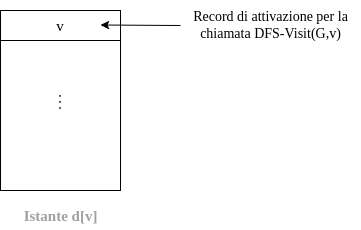
\includegraphics[scale=0.5]{res/Struttura_Parentesi1}
	\begin{tikzpicture}
		\node[rectangle,draw=black,minimum width=2cm,minimum height=2cm](stack){$\vdots$};
		\node[rectangle,draw=black,minimum width=2cm,minimum height=0.5cm,anchor=south] at (stack.north) {$v$};
		\node[gray,yshift=-0.5cm]at (stack.south) {Istante $d[v]$};
	\end{tikzpicture}
\end{center}
Più avanti con le chiamate si arriva all'istante $d[u]$ e il record di attivazione della chiamata \textsc{DFS-Visit}$(G,u)$ viene inserito in cima alla pila:
\begin{center}
	%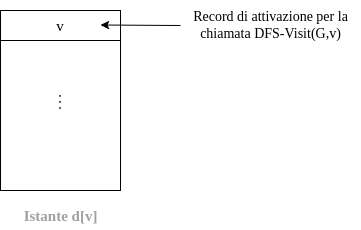
\includegraphics[scale=0.5]{res/Struttura_Parentesi1}
	\begin{tikzpicture}
		\node[rectangle,draw=black,minimum width=2cm,minimum height=2cm](stack){$\vdots$};
		\node[rectangle,draw=black,minimum width=2cm,minimum height=0.5cm,anchor=south](v) at (stack.north) {$v$};
		\node[rectangle,draw=black,minimum width=2cm,minimum height=0.5cm,anchor=south](d) at (v.north) {$\vdots$};
		\node[rectangle,draw=black,minimum width=2cm,minimum height=0.5cm,anchor=south](u) at (d.north) {$u$};
		\node[gray,yshift=-0.5cm]at (stack.south) {Istante $d[u]$};
	\end{tikzpicture}
\end{center}
A questo punto si dovrebbe assegnare l'algoritmo di fine visita del vertice $v$ e per farlo si dovrebbe avere il record della chiamata \textsc{DFS-Visit}$(G,v)$ in cima allo stack ma al suo posto c'è il record del vertice $u$. Per terminare $v$ quindi si potrebbe pensare o di aggiungere un nuovo record per \textsc{DFS-Visit}$(G,v)$ in cima allo stack oppure di rimuovere il record del vertice $u$. Entrambe le soluzioni, però, non sono ammesse in quanto, come sappiamo, ogni vertice entra nello stack una ed una sola volta ed inoltre, per rimuovere il record del vertice $u$ andrebbe prima assegnato il suo tempo di completamento (ci troviamo ancora in un istante compreso tra $d[u]$ ed $f[u]$). Per questo motivo questa sequenza è impossibile da ottenere.
\end{proof}

\begin{corolbox}[Annidamento degli intervalli dei discendenti]
	Per ogni vertice $u,v \in V$, il vertice $u$ è discendente di $v$ nella foresta DF se e soltanto se:
	\begin{equation}\label{eq:condizione_discendenza}
		d[v]<d[u]<f[u]<f[v]
	\end{equation}
\end{corolbox}
\begin{proof}
	Siano $v$ e $z$ due vertici di $V$ si supponga di avere la seguente condizione sullo stack:
\begin{center}
	\begin{tikzpicture}
		\node[rectangle,draw=black,minimum width=2cm,minimum height=2cm](stack){$\vdots$};
		\node[rectangle,draw=black,minimum width=2cm,minimum height=0.5cm,anchor=south](v) at (stack.north) {$v$};
		\node[rectangle,draw=black,minimum width=2cm,minimum height=0.5cm,anchor=south](u) at (v.north) {$z$};
	\end{tikzpicture}
\end{center}
Ciò significa che la chiamata a \textsc{DFS-Visit}$(G,v)$ ha generato la chiamata sul vertice $z$. Allora esisterà sicuramente un arco $(v,z) \in E$ che corrisponderà ad un arco nel sottografo dei predecessori. Allora sicuramente $p[z] = v$. Dato lo stack di attivazione possiamo mappare quindi ogni sequenza di vertici con una sequenza nella foresta depth first. In questo modo si dimostra che la condizione è sufficiente.

Sia ora $u$ discendente di $v$ nella foresta depth first e ragioniamo per induzione sulla lunghezza del percorso $\pi$ da $v$ ad $u$:
\begin{itemize}
	\item \textbf{Caso base:} sia $|\pi|=1$ allora esiste un solo arco tra $v$ ed $u$ e $p[u]=v$. Se $p[u]=v$ allora sicuramente si avrà la sequenza $d[v]<d[u]<f[u]<f[v]$ per il teorema della struttura parentesi.
	\item \textbf{Caso induttivo:} sia $|\pi|>1$ e sia l'implicazione valida per $|\pi| -1$. Possiamo decomporre $\pi$ in due parti: $$\pi = \underbrace{\langle v \ldots z \rangle}_{\pi'} + \langle z,u \rangle$$
	Chiaramente $\pi'$ ha lunghezza $|\pi|-1$, quindi per ipotesi induttiva vale $d[v]<d[z]<f[z]<f[v]$. Resta da capire dove si collocano gli istanti $d[u]$ e $f[u]$ all'interno di tale sequenza. Osserviamo però che l'arco $\langle z,u \rangle$ ha dimensione uno quindi $p[u]=z$ e vale:
	\begin{displaymath}
		d[v]<d[z]<d[u]<f[u]<f[z]<f[v]
	\end{displaymath}
	per il teorema della chiusura parentesi.
\end{itemize}
\end{proof}


\begin{teorbox}[del percorso bianco]
Dato un grafo $G=(V,E)$ ed eseguita una visita in profondità su $G$ allora, per ogni vertice $u,v \in V$ con $v \neq u$ vale che $u$ è discendente di $v$ nella foresta depth first se e soltanto se all'istante $d[v]$ esiste un percorso in $G$ fatto solo di vertici bianchi da $v$ ad $u$.
\end{teorbox}

\begin{proof}Abbiamo:
\begin{enumerate}
	\item[$\implies$] partiamo dall'ipotesi che il vertice $u$ diventi discendente di $v$ all'interno della foresta depth first. Bisogna dimostrare allora che esiste almeno un percorso bianco\footnote{Non è detto che questo sia unico infatti.} da $v$ ad $u$. Chiaramente, il percorso da $v$ ad $u$ nella foresta (che coincide con un percorso nel grafo) all'istante $d[v]$ è tutto bianco. Consideriamo infatti un generico vertice $z$ all'interno del percorso da $v$ ad $u$. Se $z$ è discendente di $v$ allora per il corollario \ref{eq:condizione_discendenza} vale:\[d[v]<d[z]<f[z]<f[v]\] e ciò significa che all'istante iniziale $d[v]$ tale vertice sarà per forza bianco non essendo stato ancora scoperto.

	\item[$\impliedby$] Esista un percorso bianco da $v$ a $u$ nel grafo $G$ e dimostriamo che ogni vertice in $\pi$ diventa discendente di $v$. Per assurdo, esista almeno un vertice che non sia discendente di $v$. Sia $t$ il primo vertice non discendente di $v$ incontrato lungo il percorso da $v$ ad $u$ nella foresta depth first. Se $t$ è il primo vertice non raggiungibile chiaramente il suo predecessore lo sarà, sia esso il vertice $z$. Quindi vale sicuramente: \[d[v]<d[z]<f[z]<f[v]\]
	Poiché $z$ è il predecessore di $t$ esiste un arco $(z,t)$ nella FDF. Per il teorema della struttura parentesi però, $t$ non può essere scoperto prima di $d[v]$, non può essere scoperto dopo la fine di $f[z]$ e quindi deve per forza essere scoperto dopo l'inizio di $d[v]$ il che implica che $t$ è discendente di $v$ nella foresta depth first, il che è assurdo.
\end{enumerate}
\end{proof}


\begin{osservation}
		Anche se esistesse un arco da $z$ a $t$ non si può dire che $d[z]<d[t]$ in quanto potrebbe esistere un arco da $v$ a $t$ che viene esplorato prima.
\end{osservation}

\subsection{Caratterizzazione degli archi}
Possiamo definire quattro tipi di archi in base alla foresta depth first prodotta da una visita in profondità del grafo $G$:
\begin{enumerate}
	\item \textbf{Archi d'albero:} sono gli archi nella foresta depth first. L'arco $(u,v)$ è un arco d'albero se $v$ viene scoperto la prima volta durante l'esplorazione di $(u,v)$.
	\item \textbf{Archi all'indietro:} sono quegli archi $(u,v)$ che collegano un vertice $u$ a un antenato $v$ in un albero DF. I cappi, che possono presentarsi nei grafi orientati, sono considerati archi all'indietro.
	\item \textbf{Archi in avanti:} sono gli archi $(u,v)$ (diversi dagli archi d'albero) che collegano un vertice $u$ ad un discendente $v$ in un albero DF.
	\item \textbf{Archi di attraversamento:} tutti gli altri archi. Possono connettere i vertici nello stesso albero DF, purché un vertice non sia un antenato dall'altro, oppure possono connettere i vertici di alberi DF differenti.
\end{enumerate}

Ad esempio, si consideri il  grafo mostrato in Figura \ref{fig:grafo1} e sia $1$ il primo vertice dell'insieme $V$, allora la visita in profondità genera il sottografo dei predecessori mostrato in Figura \ref{fig:fdf1} dove:
\begin{itemize}
	\item gli archi rossi sono gli archi d'albero;
	\item gli archi verde chiaro sono gli archi all'indietro;
	\item gli archi porpora sono gli archi in avanti
	\item gli archi verde scuro sono gli archi di attraversamento.
\end{itemize}

\begin{figure}[ht!]
	\centering
	\subfloat[\label{fig:grafo1}]{
	\begin{tikzpicture}
		[node/.style={circle,draw,fill=blue!25!white,minimum size=0.5cm},>=latex]
		\node[node,name=1]at(0,0){1};
		\node[node,name=2,right=3cm of 1]{2};
		\node[node,name=3,below=2cm of 1]{3};
		\node[node,name=4,below=2cm of 2]{4};
		\draw[->,purple!75!black,very thick] (1) -- (3);
		\draw[->,red,very thick] (1) -- (2);
		\draw[->,red,very thick] (4) -- (3);
		\draw[->,green,very thick] (3) -- (2);
		\draw[->,red,very thick] (2) -- (4);
		\draw[->,green,very thick](4.north east) to [out=45,in=-45] (2.south east);
		\end{tikzpicture}}
	\hfil
	\subfloat[\label{fig:fdf1}]{
		\begin{tikzpicture}
		[node/.style={circle,draw,fill=blue!25!white,minimum size=0.5cm},>=latex]
		\node[node,name=1]at(0,0){1};
		\node[node,name=2,right=2cm of 1]{2};
		\node[node,name=4,right=2cm of 2]{4};
		\node[node,name=3,right=2cm of 4]{3};
		\draw[->,red,very thick] (1) -- (2);
		\draw[->,red,very thick] (2) -- (4);
		\draw[->,red,very thick] (4) -- (3);
		\draw[->,green,very thick] (3) to [out=135,in=30] (2);
		\draw[->,green,very thick] (4.south) to [out=245,in=-45] (2.south east);
		\draw[->,purple!75!black,very thick] (1.south east) to [out=-45,in=245] (3.south west);
	\end{tikzpicture}
	}
	\caption{}
\end{figure}

Si consideri il grafo mostrato in Figura \ref{fig:grafo2}. Supposto $2$ il primo vertice del grafo, eseguendo la BFS si ottiene l'albero DF mostrato in Figura \ref{fig:df2}.

\begin{figure}[ht!]
	\centering
	\subfloat[\label{fig:grafo2}]{
	\begin{tikzpicture}
		[node/.style={circle,draw,fill=blue!25!white,minimum size=0.5cm},>=latex]
		\node[node,name=1]at(0,2){$1$};
		\node[node,name=2]at(4,2){$2$};
		\node[node,name=3]at(2,1){$3$};
		\node[node,name=4]at(6,1){$4$};
		\node[node,name=5]at(0,0){$5$};
		\node[node,name=6]at(4,0){$6$};
		\draw[->,green,very thick] (1) -- (2);
		\draw[->,green,very thick] (3) -- (2);
		\draw[->,green,very thick] (4) -- (2);
		\draw[->,green,very thick] (3) -- (6);
		\draw[->,red,very thick] (5) -- (1);
		\draw[->,red,very thick] (5) -- (3);
		\draw[->,red,very thick] (6) -- (5);
		\draw[->,red,very thick] (2) -- (6);
		\draw[->,red,very thick] (6) -- (4);
		\draw[->,green!35!black,very thick] (4) -- (3);
		\draw[->,purple!75!black,very thick] (2.210) to [bend right=35] (5.north east);
	\end{tikzpicture}}
\hfil
\subfloat[\label{fig:df2}]{
	\begin{tikzpicture}
	[node/.style={circle,draw,fill=blue!25!white,minimum size=0.5cm},>=latex]
	\node[node,name=1]at(3,0){$1$};
	\node[node,name=2]at(2,6){$2$};
	\node[node,name=3]at(1,0){$3$};
	\node[node,name=4]at(4,2){$4$};
	\node[node,name=5]at(2,2){$5$};
	\node[node,name=6]at(2,4){$6$};
	\draw[->,red,very thick] (5) -- (1);
	\draw[->,red,very thick] (5) -- (3);
	\draw[->,red,very thick] (6) -- (5);
	\draw[->,red,very thick] (2) -- (6);
	\draw[->,red,very thick] (6) -- (4);
	\draw[->,green!35!black,very thick] (4) -- (3);
	\draw[->,green,very thick] (4) to [bend right = 35] (2);
	\draw[->,green,very thick] (1) to [bend right = 35] (2);
	\draw[->,green,very thick] (3) to [bend left = 35] (6);
	\draw[->,green,very thick] (3) to [bend left = 35] (2);
	\draw[->,purple!75!black,very thick] (2) to [bend right = 35] (5);
\end{tikzpicture}
}
\caption{}
\end{figure}

L'algoritmo \textsc{DFS} può essere utilizzato per classificare gli archi di un grafo $G$. In particolare, si usa il colore del vertice che si raggiunge durante la visita dell'arco $(u,v)$ per effettuare la discriminazione tra le varie tipologie:
\begin{itemize}
	\item Se $v$ è bianco allora l'arco è un \textbf{\textcolor{red}{arco d'albero}};
	\item Se $v$ è grigio allora l'arco è un \textbf{\textcolor{green}{arco di ritorno}};
	\item Se $v$ è nero allora l'arco è un \textbf{\textcolor{purple!75!black}{arco in avanti}} o un \textbf{\textcolor{green!35!black}{arco di attraversamento}}:
	\begin{itemize}
		\item se inoltre $d[u]<d[v]$ allora è un \textbf{\textcolor{purple!75!black}{arco in avanti}};
		\item se inoltre $d[v]<d[u]$ allora è un \textbf{\textcolor{green!35!black}{arco di attraversamento}}.
	\end{itemize}
\end{itemize}
È possibile quindi modificare l'algoritmo \textsc{DFS-Visit}$(G,s)$ per visualizzare la tipologia di tutti gli archi ispezionati:
\begin{lstlisting}[language=asd,caption={Print-DFS-Visit(G,s)}]
Color[s] = Gray
time = time+1
d[s] = time
for each v @$\in$@ Adj(s) do
	if Color[v] = White then
		print("(s,v) e' d'albero")
		Pred[v] = s
		DFS-Visit(G,v)
	else
		if Color[v] = Gray then
			print("(s,v) e' all'indietro")
		else if(d[s]<d[v]) then
			print("(s,v) e' in avanti")
		else
			print("(s,v) e' d'attraversamento")
time = time+1
f[s] = time
Color[s] = Black
\end{lstlisting}

\subsection{Verifica dei grafi aciclici}
Grazie alla caratterizzazione degli archi appena visti possiamo osservare che l'algoritmo \textsc{DFS} è in grado di verificare se un grafo è \textbf{ciclico} o meno. Se si osservano attentamente i grafi mostrati in Figura \ref{fig:grafo1} e \ref{fig:grafo2} notiamo infatti la presenza di vari cicli che vengono descritti dagli archi etichettati di verde chiaro, ovvero gli archi all'indietro.

Assumiamo che $G=(V,E)$ sia un grafo orientato in cui ci sia un ciclo semplice $\langle v_{1},v_{2},\ldots,v_{k} \rangle$ e sia $v_{1}$ il primo vertice scoperto dalla \textsc{BFS}. Nell'istante $d[v_{1}]$ gli altri vertici sono bianchi, quindi, per il teorema del percorso bianco esiste un percorso bianco da $v_{1}$ a $v_{2},v_{2}, \ldots, v_{i}$ per $i=\{2,3,\ldots,k\}$. Se esiste tale percorso bianco allora i vertici $v_{2},v_{3}, \ldots, v_{i}$ sono discendenti di $v_{1}$ e gli archi di tale percorso sono archi dell'albero. Una volta arrivati al vertice $v_{k}$ l'unico arco ancora da percorrere è quello che lo conduce all'antenato $v_{1}$ e tale arco risulta quindi un arco all'indietro.
\begin{center}
	\begin{tikzpicture}
	[node/.style={circle,draw,fill=blue!25!white,minimum size=0.5cm},>=latex]
	\node[node,name=1]at(1,5){$v_{1}$};
	\node[node,name=2]at(3,6){$v_{2}$};
	\node[node,name=3]at(5,5){$v_{3}$};
	\node[node,name=4]at(5,3){$v_{4}$};
	\node[node,name=5]at(3,2){$v_{5}$};
	\node[node,name=6]at(1,3){$v_{k}$};
	\draw[->,red,very thick](1) to[bend left=35] (2);
	\draw[->,red,very thick](2) to[bend left=35] (3);
	\draw[->,red,very thick](3) to[bend left=35] (4);
	\draw[->,red,very thick](4) to[bend left=35] (5);
	\draw[->,dashed,red,very thick](5) to[bend left=35] (6);
	\draw[->,green,very thick](6) to[bend left=35] (1);
	\end{tikzpicture}
\end{center}

È possibile quindi definire un algoritmo il quale, dato un grafo orientato, restituisca \texttt{true} se aciclico e \texttt{false} altrimenti.
\begin{minipage}{.4\textwidth}
	\begin{lstlisting}[language=asd,caption={\textsc{Aciclico}(G)}]
		Init(G)
		for each v @$\in$@ V do
			if Color[v] = White then
				ret = Aciclico-Visit(G,v)
				if ret = false then
					return false
		return true
	\end{lstlisting}
\end{minipage}
\begin{minipage}{.4\textwidth}
	\begin{lstlisting}[caption={\textsc{Aciclico-Visit}(G,s)},language=asd]
		Color[s] = Gray
		for each v @$\in$@ Adj(s) do
			if Color[v] = White then
				ret = Aciclico-Visit(G,v)
				if ret = false then
					return false
			else
				if Color[v] = Gray then
					return false
		return true
	\end{lstlisting}
\end{minipage}
\newpage

\section{Ordinamento topologico in un grafo}
\subsection{Relazione d'ordine nei grafi}
\dfn{Ordinamento topologico}{
	Sia $G=(V,E)$ un grafo orientato aciclico, si definisce \textbf{ordinamento topologico} di $G$ una permutazione $\pi$ di $V$ tale che:
	\begin{equation}
		\forall (v,u) \in E, \quad \text{$v$ precede $u$ in $\pi$}
	\end{equation}
	Se due vertici $v$ e $u$ sono presenti in un ordinamento topologico allora si diranno \textit{confrontabili} e lo si indica con $v < u$.
}

\begin{example}
Si consideri il seguente grafo:
\begin{center}
	\begin{tikzpicture}
	[node/.style={circle,draw,fill=blue!25!white,minimum size=0.5cm},>=latex, level 1/.style={sibling distance=3cm},level 2/.style={sibling distance=4cm}]
\node[node]{4}
child[->]{
	node[node]{3}
	child{
		node[node,name=1]{7}
	}
	child{
		node[node,name=2]{1}
	}
}
child[->]{
	node[node]{8}
	child[missing]
	child{
		node[node]{9}
	}
};
\draw[-,dashed,red,thick](1)--node[above]{Non confrontabili}(2);
\end{tikzpicture}
\end{center}
È possibile ricavare le seguenti relazioni:
\begin{displaymath}
	\begin{array}{ll}
		4 < 3 &		4 < 8\\
		4 < 7 &		4 < 1\\
		4< 9 &		3 < 7\\
		3 < 1 &		8 < 9\\
	\end{array}
\end{displaymath}
Notare il fatto che non è possibile determinare alcuna relazione tra i vertici $7$ ed $1$ oppure $3$ ed $8$ in quanto non esiste alcun arco in $G$ che li collega. In generale, infatti, la struttura del grafo induce una relazione d'ordine \textit{parziale}.
\end{example}


\begin{osservation}
		Se nel grafo sono presenti cicli non è possibile determinare alcun ordinamento topologico. Infatti, preso ad esempio il seguente grafo:
	\begin{center}
		\begin{tikzpicture}
			[node/.style={circle,draw,fill=blue!25!white,minimum size=0.5cm},>=latex]
			\node[node,name=1]{$v_{1}$};
			\node[node,name=2,right=4cm of 1]{$v_{2}$};
			\draw[->,very thick](1.north) to[bend left=25](2.north);
			\draw[->,very thick](2.south)to[bend left=25](1.south);
		\end{tikzpicture}
	\end{center}
	non è possibile determinare quale nodo preceda l'altro all'interno di un possibile ordinamento. Lo stesso ragionamento vale anche nel caso in cui si considerano i grafi non orientati dove non è definito il concetto di precedenza. Per questo motivo, la nozione di ordinamento topologico si applica solo ai grafi orientati aciclici.
\end{osservation}


\begin{osservation}
		Dato un grafo orientato $G=(V,E)$ è possibile ricavare più di un ordinamento topologico. Nel caso in cui l'insieme $E$ sia vuoto (grafo senza archi) allora il numero di permutazioni possibili corrisponde a $|V|!$. Nel caso in cui il grafo si riduca ad una sequenza di vertici è possibile avere un unico ordinamento topologico. Si consideri ad esempio il seguente grafo:
	\begin{center}
		\begin{tikzpicture}
			[node/.style={circle,draw,fill=white,minimum size=0.5cm},>=latex]
			\node[node,name=1]at(0,0){$v_{1}$};
			\node[node,name=2]at(1,0){$v_{2}$};
			\node[node,name=3]at(2,0){$v_{3}$};
			\node[node,name=4]at(3,0){$v_{4}$};
			\node[node,name=5]at(4,0){$v_{5}$};
			\draw[->,thick] (1)--(2);
			\draw[->,thick] (2)--(3);
			\draw[->,thick] (3)--(4);
			\draw[->,thick] (4)--(5);
		\end{tikzpicture}
	\end{center}
	Tale grafo ammette un unico ordinamento topologico dato dalla permutazione $\pi=\langle v_{1},v_{2},v_{3},v_{4},v_{5} \rangle$. Tale ordinamento non è solo l'unico ma anche totale.
\end{osservation}

\subsection{Proprietà dei grafi aciclici}


\begin{propbox}
		Se $G=(V,E)$ è un grafo aciclico e $G'$ è un suo sottografo allora $G'$ è aciclico.
\end{propbox}

\begin{proof}
	Per ipotesi si ha $G' = (V',E') $, con:
\begin{displaymath}
\begin{array}{c}
			V' \subseteq V \\
			E' \subseteq E \cap (V' \times V')
\end{array}
\end{displaymath}
Supponiamo per assurdo che $G'$ sia un grafo ciclico e consideriamo un percorso ciclico di $G'$, sia esso $\pi$:
\begin{displaymath}
	\pi = \langle v_{1}, v_{2}, \cdots, v_{k}, v_{1}\rangle
\end{displaymath}
Chiaramente ciascun arco nel percorso $\pi$ è un arco presente in $E'$. Poiché $E'$ è un sottoinsieme di $E$, quindi ogni arco di $\pi$ appartiene ad $E$ e $\pi$ risulta quindi un percorso in $G$ che di fatto risulta ciclico, contro le nostre ipotesi.
\end{proof}

\begin{propbox}
	Se $G$ è un grafo aciclico allora esiste almeno un vertice $v \in V$ tale che $v$ ha grado entrante pari a $0$.
\end{propbox}


\begin{proof}
	Ragionando per contrapposizione supponiamo che per ogni vertice di $V$ ci sia almeno un arco entrante. Senza ledere di generalità consideriamo un vertice di $V$, tale $v_{1}$. Per l'ipotesi appena posta esiste almeno un arco che entra in $v_{1}$ ed esiste quindi un vertice $v_{2} \neq v_{1}$ dal quale si diparte tale arco. Ragionando allo stesso modo possiamo considerare un arco che parta da un vertice $v_{3}$ e arrivi in $v_{2}$ e così via fino ad arrivare all'ultimo vertice $v_{n} \in V$.  Poiché il grado entrante di $v_{n}$ è maggiore di $1$ ciò significa che esiste almeno un arco che parte da uno dei vertici $\{v_{1},\ldots, v_{n-1}\}$ (non potrebbe essere altrimenti) e arriva in $v_{n}$. Ciò, però, dimostra l'esistenza di un percorso ciclico nel grafo $G$, il quale per ipotesi era stato definito aciclico. Mostrato l'assurdo si dimostra l'enunciato.
\begin{center}
	\begin{tikzpicture}
		[node/.style={circle,draw,fill=blue!25!white,minimum size=0.5cm},>=latex]
		\node[node,name=1]at(0,0){$v_{1}$};
		\node[node,name=2]at(-2,0){$v_{2}$};
		\node[node,name=3]at(-4,0){$v_{3}$};
		\node[node,name=4]at(-6,0){$v_{4}$};
		\node[node,name=5]at(-9,0){$v_{k}$};
		\draw[->,thick] (2)--(1);
		\draw[->,thick] (3)--(2);
		\draw[->,thick] (4)--(3);
		\draw[->,thick,dashed] (5)--(4);
		\draw[->,red,thick](3) to [bend left=25] (5);
	\end{tikzpicture}
\end{center}
\end{proof}



\begin{propbox}
		Dato un grafo aciclico $G=(V,E)$, se $G$ è aciclico allora esiste almeno un ordinamento topologico di $G$.
\end{propbox}


\begin{proof}
	Dato che $G$ è aciclico esiste almeno un vertice $v_{1} \in V$ con grado entrante pari a zero. Chiaramente un vertice del genere deve essere posto all'inizio di qualsiasi ordinamento topologico $\pi$ in quanto non esiste alcun vertice che lo preceda. Escluso tale vertice possiamo quindi considerare il sottografo: $$G_{1}=(V\setminus\{v_{1}\},E \setminus \{(v_{1},u)\in E \; | \; u \in V\})$$ ottenuto rimuovendo $v_{1}$ da $V$ e ciascun arco che collegava $v_{1}$.
\begin{center}
	\begin{tikzpicture}
		[node/.style={circle,draw,fill=blue!25!white,minimum size=0.5cm},>=latex]
		\node[node,name=1]at(0,0){};
		\node[node,name=2]at(-3,-0.5){};
		\node[node,name=3]at(-5,-1){};
		\node[node,name=4]at(-6,0){};
		\node[node,name=5]at(-9,-1){};
		\draw[->,thick] (2)--(1);
		\draw[->,thick] (3)--(2);
		\draw[->,thick] (4)--(3);
		\draw[->,thick](4)--(2);
		\draw[->,thick,dashed] (5)--(4);
		\draw[->,thick,dashed](5)--(3);
		\node[thick,draw=blue,name=r1,shape=rectangle,fit={(1)(2)(3)(4)}]{};
		\node[below=0.2cm of r1,font=\color{blue}\bfseries]{$G_{1}$};
	\end{tikzpicture}
\end{center}
Chiaramente, essendo $G_{1}$ un sottografo di un grafo aciclico, anche $G_{1}$ risulta aciclico e quindi esisterà un vertice $v_{2}$ con grado entrante pari a zero. Tale vertice può essere quindi inserito a destra del vertice $v_{1}$ all'interno dell'ordinamento topologico $\pi$. È possibile iterare questo procedimento fino a quando non si raggiunge il sottografo vuoto, ottenendo così l'ordinamento topologico:
\[\pi = (v_{1},v_{2},\ldots, v_{k})\]
\end{proof}


\begin{proof}
	Chiaramente, l'ordinamento topologico così ottenuto dipende dalla scelta del vertice $v_{i}$ con grado entrante pari a zero il quale può essere più di uno. All'interno di uno stesso grafo, infatti, l'ordine dei vertici con grado entrante pari a zero all'interno di una permutazione è indifferente e possono quindi essere messi uno dopo o prima dell'altro.
\end{proof}

\begin{example}
	Consideriamo il seguente grafo:
	\begin{center}
		\begin{tikzpicture}
			[node/.style={circle,draw,fill=blue!25!white,minimum size=0.5cm},>=latex]
			\node[node,name=a]at(0,0){A};
			\node[node,name=b]at(3,2){B};
			\node[node,name=c]at(3,0){C};
			\node[node,name=d]at(1,-2){E};
			\node[node,name=e]at(6,0){D};
			\draw[->,thick](a) --(b);
			\draw[->,thick](b) --(c);
			\draw[->,thick](a) --(c);
			\draw[->,thick](c) --(e);
			\draw[->,thick](d) --(c);
		\end{tikzpicture}
	\end{center}
In questo caso esistono due vertici con grafo entrante pari a zero: il vertice A  ed il vertice E. Possiamo quindi scegliere uno qualsiasi tra i due come primo elemento della permutazione $\pi$. Scelto il vertice A si ottiene:
\begin{center}
	\begin{tikzpicture}
		[node/.style={circle,draw,fill=blue!25!white,minimum size=0.5cm},>=latex]
		\node[node,name=a,opacity=0.2]at(0,0){A};
		\node[node,name=b]at(3,2){B};
		\node[node,name=c]at(3,0){C};
		\node[node,name=d]at(1,-2){E};
		\node[node,name=e]at(6,0){D};
		\node[shape=rectangle,name=g1,draw=red,fit={(b)(c)(d)(e)}]{};
		\node[below=0.5cm of g1,font=\color{red}\bfseries]{$G_{1}$};
		\node[right=0.5cm of g1,font=\bfseries]{$\pi=(A)$};
		\draw[->,thick,opacity=0.2](a) --(b);
		\draw[->,thick](b) --(c);
		\draw[->,thick,opacity=0.2](a) --(c);
		\draw[->,thick](c) --(e);
		\draw[->,thick](d) --(c);
	\end{tikzpicture}
\end{center}
Il sottografo $G_{1}$ così ottenuto ha ancora due vertici con grado entrante pari a zero: B ed E. Scelto quindi il vertice E si ottiene il nuovo sottografo $G_{2}$:
\begin{center}
	\begin{tikzpicture}
		[node/.style={circle,draw,fill=blue!25!white,minimum size=0.5cm},>=latex]
		\node[node,name=a,opacity=0.2]at(0,0){A};
		\node[node,name=b]at(3,2){B};
		\node[node,name=c]at(3,0){C};
		\node[node,name=d,opacity=0.2]at(1,-2){E};
		\node[node,name=e]at(6,0){D};
		\node[shape=rectangle,name=g1,draw=red,fit={(b)(c)(e)}]{};
		\node[below=0.5cm of g1,font=\color{red}\bfseries]{$G_{2}$};
		\node[right=0.5cm of g1,font=\bfseries]{$\pi=(A,E)$};
		\draw[->,thick,opacity=0.2](a) --(b);
		\draw[->,thick](b) --(c);
		\draw[->,thick,opacity=0.2](a) --(c);
		\draw[->,thick](c) --(e);
		\draw[->,thick,opacity=0.2](d) --(c);
	\end{tikzpicture}
\end{center}
Il grafo $G_{2}$, così come il resto dei suoi sottografi ottenuti iterando il procedimento, hanno un unico vertice con grado entrante pari a zero, è quindi univoca la sequenza dei vertici estratti. Si ottiene così l'ordinamento topologico: $$\pi=(A,E,B,C,D)$$
\end{example}

\subsection{Algoritmo del grado entrante}
Per trasformare la procedura appena studiata in un algoritmo che determini un ordinamento topologico bisogna capire come calcolare il \textit{grado entrante} di ogni vertice per poter selezionare i vertici con grado entrante nullo. Le liste di adiacenza non sono adatte a fornire tale informazione in quanto esprimono (mediante la loro dimensione) soltanto il grado uscente di ogni vertice.

Chiaramente, il grado entrante di un vertice può essere ottenuto dalla dimensione della sua \textbf{lista di incidenza}, ovvero una lista che descrive tutti i vertici dai quali si dipartono degli archi orientati verso il vertice selezionato\footnote{Qualora il grafo fosse stato implementato mediante matrici di adiacenza sarebbe stato sufficiente calcolare la sua trasposta}. La generazione di tali liste, però, risulta essere un'operazione costosa in quanto richiede di scorrere l'intero insieme degli archi. Per questo motivo, si preferisce utilizzare un algoritmo che calcoli il grado entrante di ogni vertice in modo più efficiente.
% Explain how the SortingTopology algorithm works, in particular how the indegrees of each vertex are calculated.
L'Algoritmo \ref{lst:GradoEntrante} imposta innanzitutto il grado entrante di ogni vertice a $0$ e poi, per ogni vertice $v \in V$, incrementa il grado entrante di tutti i vertici adiacenti ad $v$. Chiaramente, l'algoritmo risulta essere lineare sulla dimensione del grafo.

Calcolato il grado entrante di ciascun vertice è possibile implementare l'algoritmo \ref{lst:OrdTop} che, partendo dai vertici con grado entrante pari a zero, li inserisce in una coda $Q$ e li estrae uno alla volta. Per ogni vertice estratto $v$ si itera sui suoi adiacenti $u$ e si decrementa il loro grado entrante. Se il grado entrante di $u$ diventa pari a zero allora viene inserito nella coda $Q$. L'algoritmo termina quando la coda $Q$ risulta vuota.

\begin{lstlisting}[caption={\textsc{OrdinamentoTopologico}(G)},language=asd,label=lst:OrdTop]
  Q = NIL
  // Funzione che associa ad ogni vertice il proprio grado entrante
  Ge = GradoEntrante(G)
  for each v @$\in$@ V do
    // Accodo i vertici con grado zero
    if Ge[v]=0 then
      Q = Enqueue(Q,v)
  while (Q @$\neq$@ NIL) do
    v = Head(Q)
    print(v)
    // Aggiorno il grado entrante degli adiacenti
    for each u @$\in$@ Adj[v] do
      Ge[u] = Ge[u]-1
      if Ge[u]=0 then
        Q = Enqueue(Q,u)
      Q= Dequeue(Q)
\end{lstlisting}
\begin{lstlisting}[language=asd,caption={\textsc{GradoEntrante}(G)},label=lst:GradoEntrante]
for each v @$\in$@ V do
  Ge[v] =0
for each v @$\in$@ V do
  for each u @$\in$@ Adj[v] do
    Ge[u]=Ge[u]+1
return Ge
\end{lstlisting}

Chiaramente, l'algoritmo \ref{lst:OrdTop} risulta lineare sulla dimensione del grafo. Infatti:
\begin{eqnarray*}
	T_{OrdinamentoTopologico} &=& T_{GradoEntrante} + |V| + (|V|+|E|)\\
	&=& (|V|+|E|) + |V| + (|V|+|E|) \\
	&=& 3 \cdot |V| + 2 \cdot |E| \\
	&\simeq& |V| + |E|
\end{eqnarray*}

\subsection{Calcolo dell'ordinamento topologico mediante DFS}
È possibile calcolare l'ordinamento topologico di un grafo mediante l'algoritmo \textsc{DFS} in modo molto semplice. Infatti, l'ordinamento topologico di un grafo $G$ è semplicemente l'ordinamento inverso dei tempi di fine visita dei vertici di $G$. Infatti, se $G$ è aciclico allora non esistono archi all'indietro e quindi non esistono archi che collegano vertici con tempi di fine visita diversi. Inoltre, se $G$ è aciclico allora esiste almeno un vertice con grado entrante pari a zero e quindi tale vertice sarà il primo ad essere visitato dall'algoritmo \textsc{DFS}. Il vertice successivo da visitare sarà il vertice adiacente al primo e così via. Sfruttando questa osservazione è possibile inserire i vertici in uno stack man mano che questi vengono visitati. Una volta terminata la visita, basterà estrarre i vertici dallo stack per ottenere l'ordinamento topologico. L'algoritmo \ref{lst:OrdTopDFS} mostra come implementare tale procedura.

Il tempo di esecuzione di tale algoritmo è pari a quello dell'algoritmo \textsc{DFS}. Infatti, l'unico costo aggiuntivo è quello di inserire i vertici nello stack, operazione che richiede tempo costante. L'ordinamento topologico viene quindi calcolato in tempo lineare sulla dimensione del grafo.
	\begin{lstlisting}[language=asd,caption={\textsc{OrdinamentoTopologico-DFS}(G)},label=lst:OrdTopDFS]
	tempo = 0
	Init(G)
	S = NIL
	for each v @$\in$@ V do
		if Color[v] = White then
			S = OrdinamentoTopologico-DFS-Visit(G,v,S)
	return S
\end{lstlisting}



	\begin{lstlisting}[language=asd,caption={\textsc{OrdinamentoTopologico-DFS-Visit}(G,v,S)},label=lst:OrdTopDFSVisit]
	Color[v] = Gray
	time = time+1
	d[v] = time
	for each u @$\in$@ Adj[v] do
		if Color[u] = White then
			S = OrdinamentoTopologico-DFS-Visit(G,u,S)
	time = time+1
	f[v] = time
	Color[v] = Black
	S = Push(S,v)
	return S
\end{lstlisting}


\section{Calcolo delle componenti fortemente connesse}

Il concetto di \textbf{componente fortemente connessa} è strettamente legato al concetto di grafo fortemente connesso.

\dfn{Raggiungibilità e connessione}{
	Un grafo non orientato è \textbf{connesso} se ogni coppia di vertici è collegata attraverso un cammino.  Le \textbf{componenti connesse} di un grafo è un insieme di coppie di vertici che soddisfano la condizione di raggiungibilità. Un grafo orientato è \textbf{fortemente connesso} se due vertici qualsiasi sono raggiungibili l'uno con l'altro. Se $G$ è un grafo orientato non fortemente connesso, ed il grafo non orientato sottostante è connesso, allora si dice che $G$ è \textbf{debolmente connesso}.
}

\begin{example}
	Ad esempio, il grafo non orientato $G=(V,E)$ mostrato in Figura \ref{fig:grafoconnesso1} è un grafo connesso, infatti ogni vertice è raggiungibile da qualsiasi altro vertice. Al contrario, il grafo non orientato mostrato in Figura \ref{fig:grafoconnesso2} non è un grafo connesso in quanto non tutti i vertici sono reciprocamente raggiungibili, in questo caso il grafo è detto \textbf{sconnesso}.
	\begin{center}
		\begin{minipage}{.45\textwidth}
			\centering
			\begin{tikzpicture}
			[node/.style={circle,draw,fill=blue!25!white,minimum size=0.5cm},>=latex]
			\node[node,name=1] at (0.84,4) {a};
			\node[node,name=2]at (3.12,4.96) {b};
			\node[node,name=3]at (1.38,2){c};
			\node[node,name=4]at(3.9,2.2){d};
			\node[node,name=5]at(5,3.22){e};
			\draw[-,thick](1)--(2);
			\draw[-,thick](1)--(3);
			\draw[-,thick](1)--(4);
			\draw[-,thick](2)--(4);
			\draw[-,thick](2)--(5);
			\draw[-,thick](4)--(5);
			\draw[-,thick](3)--(4);
		\end{tikzpicture}
	\captionof{figure}{}\label{fig:grafoconnesso1}
		\end{minipage}
	\begin{minipage}{.45\textwidth}
		\centering
		\begin{tikzpicture}
			[node/.style={circle,draw,fill=blue!25!white,minimum size=0.5cm},>=latex]
			\node[node,name=a] at (0.84,4) {a};
			\node[node,name=b]at (4.58,3.98) {b};
			\node[node,name=c]at (1.14,2.5){c};
			\node[node,name=d]at(3.56,2.5){d};
			\node[node,name=e]at(1.96,3.32){e};
			\node[node,name=f]at(3.04,4.38){f};
			\node[node,name=g]at(4.92,3.16){g};
			\draw[-,thick](a)--(e);
			\draw[-,thick](e)--(c);
			\draw[-,thick](c)--(a);
			\draw[-,thick](f)--(b);
			\draw[-,thick](g)--(b);
			\draw[-,thick](d)--(b);
			\draw[-,thick](d)--(f);
		\end{tikzpicture}
	\captionof{figure}{}\label{fig:grafoconnesso2}
	\end{minipage}
	\end{center}
\end{example}

\dfn{Componente fortemente connessa}{
	Una \textbf{componente fortemente connessa} di un grafo orientato $G=(V,E)$ è un insieme massimale di vertici $C \subseteq V$ tale che per ogni coppia di vertici $u,v \in C$ si ha $	u  \leadsto v $ e anche $ v \leadsto u$; ovvero i vertici $u$ e $v$ sono raggiungibili l'uno dall'altro.
}


\begin{osservation}
	Se in un grafo orientato esistono vertici mutualmente raggiungibili vuol dire che il grafo è ciclico.
\end{osservation}


\begin{example}
Si consideri il grafo $G$ in Figura \ref{fig:example_strongly_connected_graph}. Tale grafo contiene quattro componenti fortemente connesse: $C_{1},C_{2},C_{3}$ e $C_{4}$.
\begin{center}
		\begin{tikzpicture}
		[node/.style={circle,draw,fill=blue!25!white,minimum size=0.5cm},>=latex]
		\node[node,name=1]at (0,0){};
		\node[node,name=2]at(1.5,0){};
		\node[node,name=3]at(3.25,0){};
		\node[node,name=4]at(5,0){};
		\node[node,name=5]at(6,-1){};
		\node[node,name=6]at(7,0){};
		\node[node,name=7]at(2,-1.5){};
		\node[node,name=8]at(3,-2.5){};
		\node[node,name=9]at(1,-2.5){};
		\node[node,name=10]at(2,-3.5){};
		\draw[->,thick](1) to [bend left=45](2);
		\draw[->,thick](2) to [bend left=45](1);
		\draw[->,thick](2) --(3);
		\draw[->,thick](3) --(4);
		\draw[->,thick](4) --(5);
		\draw[->,thick](5) --(6);
		\draw[->,thick](6) --(4);
		\draw[->,thick](7) --(8);
		\draw[->,thick](8) --(9);
		\draw[->,thick](9) --(10);
		\draw[->,thick](10) --(7);
		\draw[->,thick](10) --(8);
		\draw[->,thick](7) --(9);
		\draw[->,thick](7) --(3);
		\draw[->,thick](1) to [bend right=30](9);
		\node[draw=green,dashed,shape=ellipse,fit={(1)(2)},name=c1]{};
		\node[anchor=south,font=\color{green}\bfseries]at(c1.north){$C_{1}$};
		\node[draw=red,dashed,shape=ellipse,fit={(3)},name=c3]{};
		\node[anchor=south,font=\color{red}\bfseries]at(c3.north){$C_{3}$};
		\node[draw=blue,dashed,shape=ellipse,fit={(4)(5)(6)},name=c4]{};
		\node[anchor=south,font=\color{blue}\bfseries]at(c4.north){$C_{4}$};
		\node[draw=orange,dashed,shape=ellipse,fit={(7)(8)(9)(10)},name=c2]{};
		\node[anchor=north,font=\color{orange}\bfseries]at(c2.south){$C_{2}$};
	\end{tikzpicture}
\captionof{figure}{Un grafo orientato $G$}\label{fig:example_strongly_connected_graph}
\end{center}
\end{example}


La relazione di reciproca raggiungibilità $RR$ in un grafo $G=(V,E)$ è una relazione di equivalenza. Infatti, essa è:
\begin{itemize}
	\item \textbf{riflessiva}: ogni vertice è raggiungibile da se stesso;
	\item \textbf{simmetrica}: se $u$ è raggiungibile da $v$ allora $v$ è raggiungibile da $u$;
	\item \textbf{transitiva}: se $u$ è raggiungibile da $v$ e $v$ è raggiungibile da $w$ allora $u$ è raggiungibile da $w$.
\end{itemize}

Per questo motivo è possibile definire le \textbf{classi di equivalenza} indotte dalla relazione di mutua raggiungibilità. Ogni classe di equivalenza è una componente fortemente connessa. Infatti, se due vertici sono mutualmente raggiungibili allora questi apparterranno alla stessa componente fortemente connessa.

\dfn{Grafo delle componenti}{
L'insieme quoziente della relazione $RR$, ovvero l'insieme di tutti gli insiemi di vertici mutualmente raggiungibili, è detto \textbf{insieme delle componenti fortemente connesse} di $G$ ed è rappresentato mediante il \textbf{grafo delle componenti} $G_{CFC}$ il quale è equivalente a $G$:

\begin{equation}
	G_{CFC}=(V_{CFC},E_{CFC})
\end{equation}

dove $V_{CFC}$ contiene un nodo per ogni componente fortemente connessa di $G$ e
\[E_{CFC} = \{(u,v) \; | \; u,v \in V_{CFC}, \exists \text{ un arco in $E$ da un vertice $u$  o un vertice $v$}\}\]
}

\begin{propbox}
	Sia $G=(V,E)$ un grafo, allora $u \in V $ è raggiungibile dal vertice $v \in V$ se e soltanto se esiste un percorso da un qualsiasi vertice della componente fortemente connessa di $u$ ad un qualsiasi vertice della componente fortemente connessa di $v$.
\end{propbox}

Data questa proprietà possiamo osservare che il \textbf{problema della raggiungibilità} tra due vertici può essere studiato decomponendolo mediante l'analisi del grafo delle componenti. Bisogna trovare quindi il modo di calcolare le componenti fortemente connesse presenti in un grafo.

\begin{example}
	Il grafo delle componenti del grafo mostrato in Figura \ref{fig:example_strongly_connected_graph} risulta:
	\begin{center}
		\begin{tikzpicture}
			[node/.style={circle,draw,minimum size=0.5cm},>=latex]
			\node[node,name=1,fill=green!25!white]at(0,0){$C_{1}$};
			\node[node,name=2,fill=red!25!white]at(2,0){$C_{3}$};
			\node[node,name=3,fill=blue!25!white]at(4,0){$C_{4}$};
			\node[node,name=4,fill=orange!25!white]at(1,-1.5){$C_{2}$};
			\draw[->,thick](1)--(2);
			\draw[->,thick](2)--(3);
			\draw[->,thick](4)--(2);
			\draw[->,thick](1)--(4);
		\end{tikzpicture}
	\end{center}
il che rappresenta una forma molto più compatta, che preserva ancora le informazioni relative alla raggiungibilità dei vertici, del grafo $G$.
\end{example}


\warning{Attenzione}{
	Il grafo delle componenti è \textbf{sempre aciclico}. Infatti, se esistesse un ciclo tra due componenti fortemente connesse queste apparterrebbero alla stessa classe di equivalenza del grafo connesso.
}


Nei grafi orientati, la relazione di equivalenza di raggiungibilità e reciproca raggiungibilità non si equivalgono. Si osservino infatti i seguenti grafi, nella loro versione orientata e non:
	\begin{center}
		\begin{minipage}{.45\textwidth}
			\centering
			\begin{tikzpicture}
				[node/.style={circle,draw,fill=blue!25!white,minimum size=0.5cm}]
				\node[node,name=1] at (0,1) {1};
				\node[node,name=2] at (1,1) {2};
				\node[node,name=3] at (2,0.5) {3};
				\node[node,name=5] at (0,0) {5};
				\node[node,name=4] at (1,0) {4};
				\draw[thick] (1)--(2);
				\draw[thick] (1)--(5);
				\draw[thick] (2)--(3);
				\draw[thick] (2)--(4);
				\draw[thick] (2)--(5);
				\draw[thick] (3)--(4);
				\draw[thick] (5)--(4);
			\end{tikzpicture}
			\captionof{figure}{{Grafo non orientato $A$}}
		\end{minipage}
		\hfil
		\begin{minipage}{.45\textwidth}
			\centering
			\begin{tikzpicture}
				[node/.style={circle,draw,fill=blue!25!white,minimum size=0.5cm}]
				\node[node,name=1] at (0,1) {1};
				\node[node,name=2] at (1,1) {2};
				\node[node,name=3] at (2,0.5) {3};
				\node[node,name=5] at (0,0) {5};
				\node[node,name=4] at (1,0) {4};
				\draw[thick,->] (1)--(2);
				\draw[thick,->] (1)--(5);
				\draw[thick,->] (2)--(3);
				\draw[thick,->] (2)--(4);
				\draw[thick,->] (5)--(2);
				\draw[thick,->] (4)--(3);
				\draw[thick,->] (5)--(4);
			\end{tikzpicture}
			\captionof{figure}{{Grafo orientato $B$ }}
		\end{minipage}
	\end{center}
	In un grafo non orientato ogni coppia di vertici collegati da un arco è mutualmente raggiungibile non essendo determinato alcuna orientazione e si ha $R=RR$. Al contrario, se si osserva il grafo $B$ si può osservare che i soli ed unici vertici mutualmente raggiungibili sono i singoli vertici. Cioè:
	\begin{displaymath}
		\begin{array}{l}
			R = \{(1,2),(1,5),(5,2),(2,4),(2,3),(4,3),(1,1),(2,2),(3,3),(4,4),(5,5),(5,3),(1,4),(1,3)\}\\
			RR=\{(1,1),(2,2),(3,3),(4,4),(5,5)\}
		\end{array}
	\end{displaymath}
	e vale $RR \subseteq R$. Nei grafi non orientati è sufficiente quindi verificare la raggiungibilità tra due vertici per sapere se appartengono alla stessa componente fortemente connessa.


\begin{osservation}
	Poiché la relazione di reciproca raggiungibilità determina una partizione nell'insieme dei vertici $V$ di un grafo $G$, è possibile considerare, per ogni vertice $v \in V$, il sottografo $CFC(v)$ (che corrisponde ad una classe di equivalenza), ovvero la componente fortemente connessa che contiene $v$ tra i suoi vertici (un vertice del grafo delle componenti). Chiaramente vale $CFC(v) = (V_{v},E_{v})$ dove:
\begin{displaymath}
	V_{v} = \{u \in V \; | \; \text{$u$ è reciprocamente raggiungibile con $v$}\}
\end{displaymath}
ed:
\begin{displaymath}
	E_{v}= E \cap (V_{u} \times V_{u})
\end{displaymath}
Per costruire il grafo delle componenti quindi è sufficiente trovare l'insieme $V_{v}$ (il calcolo dell'insieme $E_{v}$ è banale una volta determinato $V_{v}$) per ogni vertice del grafo $G$. Ogni componente fortemente connessa rappresenta infatti un \textbf{sottografo indotto} dalla scelta dei suoi vertici.
\end{osservation}

\subsection{Calcolo delle componenti connesse in un grafo non orientato}
Dato un grafo non orientato $G$, è possibile pensare di applicare una visita in profondità (Algoritmo \ref{lst:dfs_graph}) per risolvere il problema della raggiungibilità (e per l'osservazione precedente anche il problema della mutua raggiungibilità). Tipicamente, infatti, la DFS costruisce su $G$ una foresta, chiamata Foresta Depth First (FDF) o anche sottografo dei predecessori, costituita da alberi DF (Depth First). 

Chiaramente, tutti i vertici che appartengono ad uno stesso albero DF formano una componente connessa del grafo $G$. Possiamo quindi pensare di mappare ciascun vertice con il rispettivo albero DF di appartenenza (numerati da 1 a $k$), ottenendo così la corrispondenza che associa a ciascun vertice il ``numero'' dell'albero DF di appartenenza:
\begin{displaymath}
	CC : V \longrightarrow \mathbb{N}
\end{displaymath}
e ricavare in questo modo, per ogni $v \in V$ l'insieme $V_{v}$ ricercato.
\begin{displaymath}
	V_{v} = \{u \in V \; | \; CC[u] = CC[v] \}
\end{displaymath}

Sarà quindi sufficiente modificare l'algoritmo \textsc{DFS-Visit} in modo tale che, per ogni vertice scoperto lungo l'esplorazione del grafo, gli si associ il numero dell'albero DF che si sta attualmente costruendo.

Notiamo che la complessità temporale del meccanismo appena descritto sarà dato dal tempo della DFS che è lineare sul grafo $G$ più il tempo necessario a costruire l'insieme $V_{v}$ ovvero $k \cdot |V|$ al quale si aggiunge un costo $k \cdot |E|$ per la costruzione dei sottografi:
\begin{displaymath}
	T_{DFS_{CC}} = |V|+|E| + \bigl((k \cdot |V|) + (k\cdot|E|)\bigr)
\end{displaymath}
dove $k$ rappresenta il numero totale di componenti connesse ottenute e vale:
\begin{displaymath}
	1 \leq k \leq |V|
\end{displaymath}

\subsection{Proprietà delle componenti fortemente connesse}
\begin{teorbox}
	Se due vertici compaiono nella stessa componente fortemente connessa, allora nessun percorso tra i due vertici esce da quella componente.
\end{teorbox}

\begin{proof}
	Siano $u$ e $v$ due vertici appartenenti alla stessa componente fortemente connessa. Allora esistono percorsi sia da $v$ a $u$ che da $u$ a $v$. Sia $w$ un vertice lungo qualche percorso $	u \leadsto w \leadsto v$. Poiché c'è un percorso $v \leadsto u$, $u$ è raggiungibile da $w$ tramite $w \leadsto v \leadsto u$. Quindi $w$ e $u$ sono nella stessa componente fortemente connessa. Dall'arbitrarietà di $w$ segue l'enunciato.
\end{proof}

\begin{teorbox}
		In ogni visita DFS, tutti i vertici nella stessa componente fortemente connessa compaiono nello stesso albero depth first.
\end{teorbox}

\begin{proof}
	Sia $r$ il primo vertice di una componente fortemente connessa, visitato da \textsc{DFS} (Algoritmo \ref{lst:dfs_graph}). Poiché esso è il primo vertice ad essere scoperto allora, per il Teorema del percorso bianco (vedi \ref{sez:prop_dfs}), tutti gli altri vertici nella componente fortemente connessa devono essere ancora bianchi.

Chiaramente, per definizione di componente fortemente connessa, esiste un percorso da $r$ a tutti gli altri vertici della componente fortemente connessa. Infatti questi percorsi non escono mai dalla componente fortemente connessa di $r$ per il teorema precedente e i vertici di tutti i percorsi nella componente fortemente connessa sono bianchi. Quindi, per il teorema del percorso bianco, ogni vertice nella componente fortemente connessa sarà un discendente di $r$ nell'albero depth first.
\end{proof}

\subsection{Calcolo delle componenti fortemente connesse in un grafo orientato}
Grazie alle proprietà della visita in profondità, il calcolo delle componenti connesse risulta immediato nei grafi non orientati in quanto è stato sufficiente associare ad ogni vertice il numero dell'albero DF di appartenenza ed in base a tale numero costruire i vari sottografi $CFC(v)$.

Stessa cosa non si può dire per i grafi orientati in quanto la visita in profondità da sola non è in grado di fornire le informazioni necessarie per calcolare le componenti fortemente connesse. Infatti, il sottografo dei predecessori descrive soltanto quali vertici possono essere raggiunti dal vertice che li scopre ma non il viceversa.

Dal Teorema 2, però, osserviamo che una componente connessa non può essere divisa in due alberi DF. Quindi tutti e soli i vertici appartenenti alla componente fortemente connessa della radice si troveranno sempre e solo in unico albero depth first. Chiaramente, in un singolo albero depth first è possibile avere più componenti fortemente connesse. Per identificare una componente fortemente connessa all'interno di un albero depth first è necessario sapere quali vertici dell'albero possono raggiungere la radice $r$ dell'albero DF $T_{r}$ che li ha scoperti:
\begin{displaymath}
	CFC(r) = \{ v \in T_{r} \; | \; v \leadsto r \}
\end{displaymath}
Una volta identificata la componente fortemente connessa della radice basterà separare i vertici così ottenuti dal resto dell'albero $T_{r}$ e considerare il sottoalbero $T_{r'}$ che si ottiene rimuovendo i vertici della componente fortemente connessa e ripetere il ragionamento con la nuova radice così ottenuta.

\begin{example}
Si consideri il seguente grafo orientato mostrato in Figura \ref{fig:grafo_orientato_cfc}. Eseguendo una visita in profondità si ottengono gli alberi DF mostrati in Figura \ref{fig:grafo_orientato_cfc1} e \ref{fig:grafo_orientato_cfc2}.
\begin{center}
	\begin{minipage}{.33\textwidth}
		\centering
			\begin{tikzpicture}
			[node/.style={circle,draw,minimum size=0.5cm,fill=blue!25!white},>=latex]
			\node[node,name=a] at (0.84,4) {a};
			\node[node,name=b]at (4.58,3.98) {b};
			\node[node,name=c]at (1.14,2.5){c};
			\node[node,name=d]at(3.56,2.5){d};
			\node[node,name=e,fill=red!25!white]at(1.96,3.32){e};
			\node[node,name=f,fill=red!25!white]at(3.04,4.38){f};
			\node[node,name=g]at(4.92,3.00){g};
			\draw[->,thick](e)--(a);
			\draw[->,thick](c)--(e);
			\draw[->,thick](a)--(c);
			\draw[->,thick](f)--(b);
			\draw[->,thick](b)--(g);
			\draw[->,thick](b)--(d);
			\draw[->,thick](d)--(f);
		\end{tikzpicture}
		\captionof{figure}{}\label{fig:grafo_orientato_cfc}
	\end{minipage}
\hfil
	\begin{minipage}{.3\textwidth}
	\centering
		\begin{tikzpicture}
			[node/.style={circle,draw,minimum size=0.5cm,fill=blue!25!white},>=latex]
			\node[node,name=e,fill=red!25!white]{e}
			child[->,thick]{
				node[node,name=a]{a}
				child[->,thick]{
					node[node,name=c]{c}
				}
			};
			\draw[->,green,thick](c)to [bend right = 30] (e);
		\end{tikzpicture}
	\captionof{figure}{}\label{fig:grafo_orientato_cfc1}
	\end{minipage}
	\hfil
	\begin{minipage}{.3\textwidth}
	\centering
		\begin{tikzpicture}
			[node/.style={circle,draw,minimum size=0.5cm,fill=blue!25!white},>=latex]
			\node[node,name=f,fill=red!25!white]{f}
			child[->,thick]{
				node[node,name=b]{b}
				child[thick,->]{
					node[node,name=d]{d}
				}
				child[->,thick]{
					node[node,name=g]{g}
				}
			};
			\draw[->,green,thick](d)to [bend left = 30] (f);
		\end{tikzpicture}
	\captionof{figure}{}\label{fig:grafo_orientato_cfc2}
	\end{minipage}
\end{center}
	Nel primo albero si osserva che tutti i vertici possono raggiungere la radice $e$ e vale quindi $CFC(e)=\{a,e,c\}$. Nel secondo albero, invece, solo i vertici $b$ e $d$ sono in grado di raggiungere la radice $f$ e vale quindi $CFC(f)=\{b,d,f\}$ mentre il vertice $g$ rappresenta la seconda CFC presente nell'albero, $CFC(g)=\{g\}$.
\end{example}

Per calcolare quali vertici sono in grado di raggiungere la radice $r$ di un albero DF in maniera efficiente è possibile utilizzare il concetto di \textbf{grafo trasposto}.

\dfn{Grafo trasposto}{
Si consideri un grafo orientato $G=(V,E)$, si definisce \textbf{grafo trasposto} il grafo il grafo $G^{T}=(V,E^{T})$ ottenuto invertendo l'orientamento degli archi del grafo $G=(V,E)$.
\begin{displaymath}
	E^{T} = \{(u,v) \; : \; (v,u) \in E \}
\end{displaymath}
}

\begin{example}
	Considerato il grafo $G$ visto nella Figura \ref{fig:grafo_orientato_cfc}, il grafo trasposto $G^{T}$ risulta:
\begin{center}
	\begin{tikzpicture}
			[node/.style={circle,draw,minimum size=0.5cm,fill=blue!25!white},>=latex]
			\node[node,name=a] at (0.84,4) {a};
			\node[node,name=b]at (4.58,3.98) {b};
			\node[node,name=c]at (1.14,2.5){c};
			\node[node,name=d]at(3.56,2.5){d};
			\node[node,name=e,fill=red!25!white]at(1.96,3.32){e};
			\node[node,name=f,fill=red!25!white]at(3.04,4.38){f};
			\node[node,name=g]at(4.92,3.00){g};
			\draw[->,thick](a)--(e);
			\draw[->,thick](e)--(c);
			\draw[->,thick](c)--(a);
			\draw[->,thick](b)--(f);
			\draw[->,thick](g)--(b);
			\draw[->,thick](d)--(b);
			\draw[->,thick](f)--(d);
		\end{tikzpicture}
		\captionof{figure}{}\label{fig:grafo_orientato_cfc_trasposto}
\end{center}
\end{example}


\begin{teorbox}
		Se in un grafo orientato $G$ esiste un cammino da $u$ a $v$, allora in $G^{T}$ esiste un cammino da $v$ a $u$, e viceversa.
\end{teorbox}


\begin{corolbox}
		Se $G$ è un grafo orientato e $G^{T}$ è il grafo trasposto di $G$, allora per ogni vertice $v$ di $G$ vale:
	\begin{displaymath}
		CFC(v) = CFC^{T}(v)
	\end{displaymath}
\end{corolbox}

Dato il risultato descritto dal Teorema 3 si potrebbe pensare di applicare una DFS nel grafo $G^{T}$ a partire dalle radici $r_{i}$ degli alberi depth first ottenuti dalla DFS sul grafo $G$ in modo tale da trovare i vertici che raggiungono tali vertici $r_{i}$. Non è detto però a priori che i vertici così raggiunti appartengano alla stessa componente fortemente connessa del vertice $r_{i}$.

Infatti è possibile che la visita DFS nel grafo trasposto a partire da un vertice $r_{i}$ possa saltare da un albero depth first\footnote{Della prima visita DFS nel grafo $G$} all'altro.
Si consideri ad esempio il  grafo mostrato in Figura \ref{fig:dfs_cfc_2}. Applicando una visita in profondità a partire dal vertice $a$ si ottengono due alberi depth first  come mostrato in Figura \ref{fig:dfs_cfc_df2}:

\begin{center}
	\begin{minipage}{.45\textwidth}
		\centering
		\begin{tikzpicture}
	[node/.style={circle,draw,minimum size=0.5cm,fill=blue!25!white},>=latex]
	\node[node,fill=red!75!white,name=a]at (0.5,4){a};
	\node[node,name=b,below=0.5cm of a]{b};
	\node[node,name=c,right=1cm of b]{c};
	\node[node,name=d]at(3,4){d};
	\node[node,name=e]at(4,3){e};
	\draw[->,thick](a) --(b);
	\draw[->,thick](b)--(c);
	\draw[->,thick](c)--(a);
	\draw[->,thick](d)--(c);
	\draw[->,thick](d)--(e);
	\draw[->,thick](e)to[bend right=30](d);
	\end{tikzpicture}
\captionof{figure}{}\label{fig:dfs_cfc_2}
	\end{minipage}
\hfil
	\begin{minipage}{.45\textwidth}
		\centering
		\begin{tikzpicture}
			[node/.style={circle,draw,minimum size=0.5cm,fill=blue!25!white},>=latex]
			\node[node,name=a,fill=red!75!white]{a}
			child[->,thick]{
			node[node,name=b]{b}
			child[->,thick]{
			node[node,name=c]{c}
		}
		};
	\draw[->,thick,green](c) to[bend right =30](a);

		\node[node,name=d,fill=red!75!white,right=3cm of a]{d}
		child[->,thick]{
		node[node,name=e]{e}
	};
\draw[->,thick,green](e) to[bend right=30](d);
\draw[->,thick,green!35!black](d)to[bend right=10](c);
	\end{tikzpicture}
\captionof{figure}{}\label{fig:dfs_cfc_df2}
\end{minipage}
\end{center}

Calcolando il grafo trasposto e applicando la DFS sul vertice $a$ si ottiene un solo albero depth first che contiene due componenti fortemente connesse (vedi Figura \ref{fig:df4}).
\begin{center}
\begin{minipage}{.3\textwidth}
	\centering
		\begin{tikzpicture}
		[node/.style={circle,draw,minimum size=0.5cm,fill=blue!25!white},>=latex]
		\node[node,fill=red!75!white,name=a]at (0.5,4){a};
		\node[node,name=b,below=0.5cm of a]{b};
		\node[node,name=c,right=1cm of b]{c};
		\node[node,name=d]at(3,4){d};
		\node[node,name=e]at(4,3){e};
		\draw[->,thick](b) --(a);
		\draw[->,thick](c)--(b);
		\draw[->,thick](a)--(c);
		\draw[->,thick](c)--(d);
		\draw[->,thick](e)--(d);
		\draw[->,thick](d)to[bend left=30](e);
	\end{tikzpicture}
\captionof{figure}{Grafo trasposto}
\end{minipage}
\hfil
\begin{minipage}{.3\textwidth}
	\centering
	 	\begin{tikzpicture}
 		[node/.style={circle,draw,minimum size=0.5cm,fill=blue!25!white},>=latex]
 		\node[node,name=a]{a}
 		child[->,thick]{
 			node[node]{c}
 			child{
 				node[node,name=b]{b}
 			}
 			child{
 				node[node,name=d]{d}
 				child{
 					node[node,name=e]{e}
 				}
 			}
 		};
 	\draw[->,thick,green](e)to[bend right=30](d);
 	\draw[->,thick,green](b)to[bend left=30](a);
 	\end{tikzpicture}
 \captionof{figure}{}\label{fig:df4}
\end{minipage}
 \end{center}

La sola visita del grafo trasposto non risolve da solo il problema della mutua raggiungibilità per colpa dell'arco di attraversamento $\langle d,c\rangle$. Infatti, collegando due alberi DF diversi si stanno connettendo vertici di componenti fortemente connesse diverse\footnote{Il che è totalmente possibile ma non aiuta nel nostro tentativo di limitare la ricerca dei vertici mutualmente raggiungibili ai soli vertici di un singolo albero depth first.}. Bisogna trovare quindi un modo per inibire tali archi, fare in modo cioè che, quando la DFS (applicata sul grafo trasposto) li trova, non li segua\footnote{Non è pensabile eliminarli in quanto questo tipo di operazione altererebbe il grafo. Si ricordi, però, che nella BFS, i percorsi seguiti percorrono soltanto vertici bianchi e grigi. Basterà quindi assicurarsi che tali archi puntino a vertici neri.}.

Osserviamo innanzitutto che un arco di attraversamento, se esiste, segue sempre un verso opposto rispetto ai tempi di scoperta dei vari alberi depth first. Ovvero, dati due alberi depth first con radici in $r_{j}$ e $r_{i}$ con $j<i$, un eventuale arco di attraversamento andrà sempre all'indietro come mostrato in figura:
\begin{center}
	\begin{tikzpicture}
		[triangle/.style={isosceles triangle,draw,shape border rotate=90,isosceles triangle stretches=true, minimum height=20mm,minimum width=2cm,fill=blue!25!white},node/.style={circle,draw,minimum size=0.5cm,fill=blue!25!white},>=latex]
		\node[name=r2,right=2cm of r1]{$r_{1}$};
		\node[triangle,anchor=north] at (r2.south){};
		\node[name=r3,right=2cm of r2]{$r_{2}$};
		\node[triangle,anchor=north] at (r3.south){};
		\node[name=r4,right=2cm of r3]{$r_{3}$};
		\node[triangle,anchor=north] at (r4.south){};
		\node[name=r5,right=2cm of r4]{$r_{4}$};
		\node[triangle,anchor=north,name=t5] at (r5.south){};
		\node[anchor=west,right=1cm of t5.center]{$\ldots$};
		\node[name=r6,right=2cm of r5]{$r_{k-1}$};
		\node[triangle,anchor=north,name=t6] at (r6.south){};
		\node[name=r7,right=2cm of r6]{$r_{k}$};
		\node[triangle,anchor=north,name=t7] at (r7.south){};
		\node[node,name=b,fill=white]at(t7.center){};
		\node[node,name=n,fill=black]at(t6.center){};
		\draw[->,thick,green!35!black](b)to[bend right=30](n);
		\draw[->,thick](2,-3)--(17,-3)node[anchor=north]{Tempo};
	\end{tikzpicture}
\captionof{figure}{Foresta depth first generata da una visita in profondità su un grafo}\label{fig:arco_attraversamento}
\end{center}
Ovviamente, se nel grafo $G$ gli archi di attraversamento collegano alberi nuovi ad alberi vecchi, eseguendo una visita in profondità sul grafo trasposto si avrà un'inversione della direzione di tali archi (che andranno quindi da alberi depth first vecchi ad alberi depth first nuovi).

\begin{center}
	\begin{tikzpicture}
		[triangle/.style={isosceles triangle,draw,shape border rotate=90,isosceles triangle stretches=true, minimum height=20mm,minimum width=2cm,fill=pink!25!white},node/.style={circle,draw,minimum size=0.5cm,fill=blue!25!white},>=latex]
		\node[name=r2,right=2cm of r1]{$r_{1}$};
		\node[triangle,anchor=north] at (r2.south){};
		\node[name=r3,right=2cm of r2]{$r_{2}$};
		\node[triangle,anchor=north] at (r3.south){};
		\node[name=r4,right=2cm of r3]{$r_{3}$};
		\node[triangle,anchor=north] at (r4.south){};
		\node[name=r5,right=2cm of r4]{$r_{4}$};
		\node[triangle,anchor=north,name=t5] at (r5.south){};
		\node[anchor=west,right=1cm of t5.center]{$\ldots$};
		\node[name=r6,right=2cm of r5]{$r_{k-1}$};
		\node[triangle,anchor=north,name=t6] at (r6.south){};
		\node[name=r7,right=2cm of r6]{$r_{k}$};
		\node[triangle,anchor=north,name=t7] at (r7.south){};
		\node[node,name=b,fill=white]at(t7.center){};
		\node[node,name=n,fill=black]at(t6.center){};
		\draw[->,thick,green!35!black](n)to[bend left=30](b);
		\draw[->,thick](2,-3)--(17,-3)node[anchor=north]{Tempo};
	\end{tikzpicture}
	\captionof{figure}{Direzione degli archi di attraversamento nel grafo trasposto}
\end{center}

Al termine dell'esplorazione di tutti i vertici bianchi raggiungibili da una sorgente $s$, l'Algoritmo \textsc{DFS\_Visit}$(G,s)$ (Algoritmo \ref{lst:dfs_visit_graph}) lo colora di nero. Questo significa quindi che un arco di attraversamento come mostrato nella Figura \ref{fig:arco_attraversamento} va sempre da vertici colorati di bianco a vertici colorati di nero\footnote{Questo in quanto gli alberi $T_{r_{k}}$ vengono costruiti sempre e solo dopo la terminazione della costruzione dell'albero $T_{r_{k-1}}$.}. Chiaramente, nel caso di una DFS nel grafo trasposto l'esatto contrario: un arco di attraversamento collega sempre un vertice nero ad un vertice bianco.

\begin{center}
	\begin{tikzpicture}
		[triangle/.style={isosceles triangle,draw,shape border rotate=90,isosceles triangle stretches=true, minimum height=20mm,minimum width=2cm,fill=pink!25!white},node/.style={circle,draw,minimum size=0.5cm,fill=blue!25!white},>=latex]
		\node[name=r2,right=2cm of r1]{$r_{1}$};
		\node[triangle,anchor=north] at (r2.south){};
		\node[name=r3,right=2cm of r2]{$r_{2}$};
		\node[triangle,anchor=north] at (r3.south){};
		\node[name=r4,right=2cm of r3]{$r_{3}$};
		\node[triangle,anchor=north] at (r4.south){};
		\node[name=r5,right=2cm of r4]{$r_{4}$};
		\node[triangle,anchor=north,name=t5] at (r5.south){};
		\node[anchor=west,right=1cm of t5.center]{$\ldots$};
		\node[name=r6,right=2cm of r5]{$r_{k-1}$};
		\node[triangle,anchor=north,name=t6] at (r6.south){};
		\node[name=r7,right=2cm of r6]{$r_{k}$};
		\node[triangle,anchor=north,name=t7,fill=black!50] at (r7.south){};
		\node[node,name=n,fill=white]at(t6.center){};
		\draw[->,thick,green!35!black](n)to[bend left=30](t7.center);
		\draw[->,thick](2,-3)--(17,-3)node[anchor=north]{Tempo};
	\end{tikzpicture}
	\captionof{figure}{}
\end{center}

Prendiamo quindi l'albero $T_{r_{k}}$ e consideriamo di eseguire una DFS applicata sul grafo trasposto. Chiaramente, essendo tale albero l'ultimo costruito nella prima DFS, non possono esistere altri alberi in cui un eventuale arco di attraversamento possa puntare andando in avanti. Per questo motivo l'applicazione dell'Algoritmo \textsc{DFS\_Visit}$(G^{T},r_{k})$ può solo raggiungere vertici dell'albero $T_{r_{k}}$. Terminata tale procedura tutti i vertici (per semplicità) di $T_{r_{k}}$ saranno colorati di nero. A questo punto \textsc{DFS\_Visit}$(G^{T},r_{k-1})$ vedrà inibiti gli archi di attraversamento che puntano a $T_{r_{k}}$.

Essendo l'albero $T_{r_{k}}$ l'ultimo albero della foresta depth first ottenuta nella prima DFS si avrà che il vertice $r_{k}$ sarà il vertice che avrà il massimo tempo di fine visita, sarà ovvero l'ultimo vertice ad essere eliminato dallo stack. Per inibire, quindi, gli archi di attraversamento sarà sufficiente eseguire l'algoritmo \textsc{DFS\_Visit} selezionando i vertici in ordine inverso rispetto ai tempi di fine visita ottenuti nella prima DFS.

Possiamo dunque pensare di modificare l'Algoritmo DFS in modo tale da salvare in uno stack i vertici in ordine di tempo di fine visita. In questo modo, una volta terminata la prima DFS, sarà sufficiente eseguire una seconda DFS sul grafo trasposto in ordine inverso rispetto ai tempi di fine visita ottenuti nella prima DFS. Ogni albero depth first ottenuto in questa seconda visita corrisponderà ad una componente fortemente connessa del grafo $G$.

\begin{minipage}{.45\textwidth}
	\begin{lstlisting}[caption={\textsc{DFS}(G)}, label={lst:dfs_cfc},language=asd]
S = @$\emptyset$@
Init(G)
for each v @$\in$@ V do
	if Color[v] = White then
		S = DFS_Visit(G,v,S)
return S
\end{lstlisting}
\end{minipage}
\hfil
\begin{minipage}{.45\textwidth}
	\begin{lstlisting}[caption={\textsc{DFS\_Visit}(G,v,S)}, label={lst:dfs_visit_cfc},language=asd]
Color[v] = Gray
for each u @$\in$@ Adj[v] do
	if Color[u] = White then
		S = DFS_Visit(G,u,S)
S = Push(S,v)
Color[v] = Black
return S
\end{lstlisting}
\end{minipage}

\begin{minipage}{.45\textwidth}
	\begin{lstlisting}[caption={\textsc{DFS2}($G^{T}$,S)},language=asd]
Init(@$G^{T}$@)
while (S @$\neq \emptyset$@)
	v = Top(S)
	if Color[v] = White then
		DFS_Visit2(@$G^{T}$@,v)
	S = Pop(S)
\end{lstlisting}
\end{minipage}
\hfil
\begin{minipage}{.45\textwidth}
	\begin{lstlisting}[caption={\textsc{DFS\_Visit2}($G^{T}$,v)},language=asd]
	Color[v] = Gray
	for each u @$\in$@ Adj[v] do
		if Color[u] = White then
			Pred[u] = v
			DFS_Visit2(@$G^{T}$@,u)
\end{lstlisting}
\end{minipage}

\begin{lstlisting}[caption={\textsc{CFC}(G)},language=asd]
S = DFS(G)
@$G^{T}$@ = GrafoTrasposto(G)
DFS2(@$G^{T}$@ ,S)
\end{lstlisting}

Il calcolo del grafo trasposto si può ottenere calcolando la matrice trasposta della matrice di adiacenza oppure, nel caso delle liste di adiacenza costruendo delle nuove liste a partire da quelle del grafo $G$:
\begin{lstlisting}[caption={\textsc{GrafoTrasposto}(G)},language=asd]
@$V^{T}$@  = @$\emptyset$@
for each v  @$\in$@ V
	@$V^{T}$@ = @$V^{T}$@  @$\cup$@ {v}
for each v @$\in$@ V do
	for each u @$\in$@ Adj[v] do
		@$Adj^{T}$@[u] = InserisciInTesta(@$Adj^{T}$@[u],v)
return (@$V^{T},Adj^{T}$@)
\end{lstlisting}
È immediato osservare che l'algoritmo \textsc{CFC}$(G)$ ha una complessità lineare sulla dimensione del grafo $G$.

\section{Cammini minimi nei grafi}
Lo studente Ciro Esposito deve andare a sostenere lo scritto di Algoritmi e Strutture Dati che si terrà in un'aula della sede di Ingegneria a Piazzale Tecchio ma come al solito la Circumvesuviana lo ha fatto fare tardi. Non appena arrivato alla stazione centrale di Napoli si pone il problema di trovare la strada più corta possibile dalla stazione a Fuorigrotta e così apre Google Maps per vedere i vari percorsi disponibili e cercare quello più breve.

Come mostrato in Figura \ref{fig:maps} l'applicazione associa a ciascun percorso un tempo di percorrenza ottenuto sommando i tempi di percorrenza necessari ad attraversare i vari punti lungo il percorso. Riuscirà il nostro studente ad arrivare in tempo?
\begin{center}
	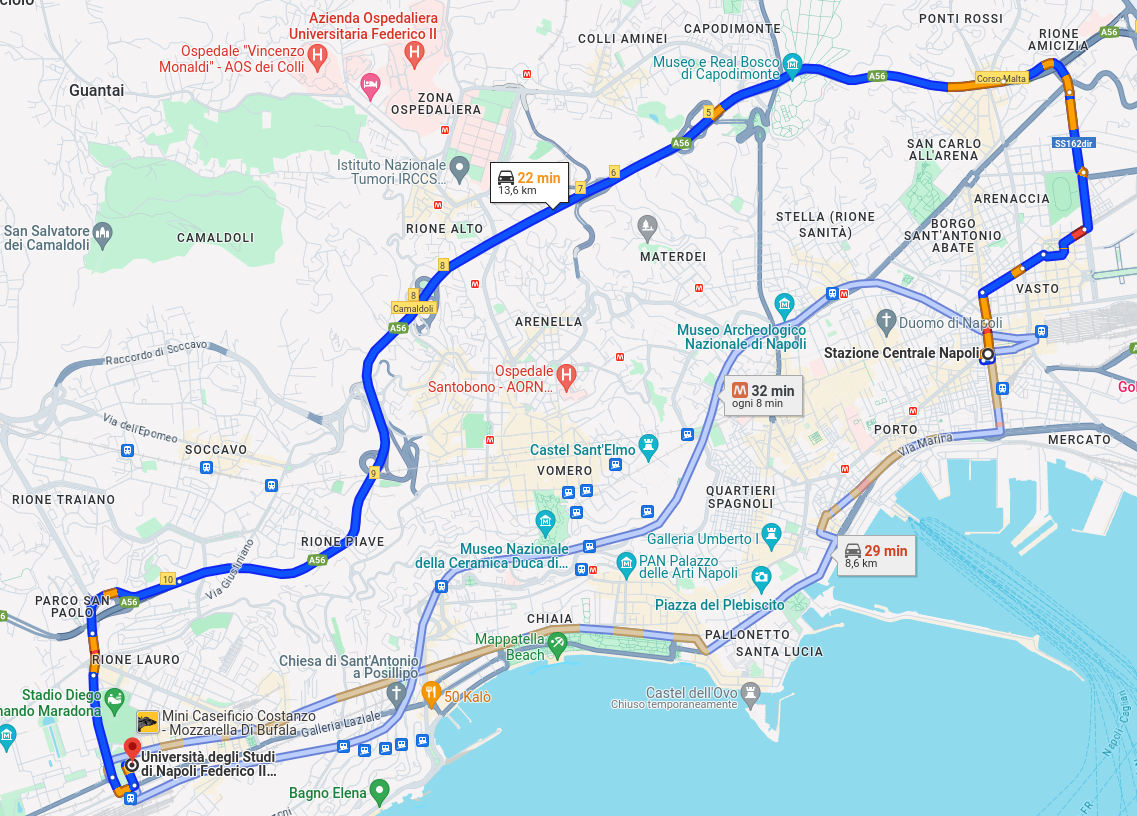
\includegraphics[scale=.45]{res/Maps}
	\captionof{figure}{I possibili percorsi per raggiungere la sede di Piazzale Tecchio a partire dalla stazione Centrale di Napoli}\label{fig:maps}
\end{center}

\subsection{I grafi pesati}
Per risolvere questa tipologia di problema che attanaglia migliaia di studenti ritardatari si fa uso del concetto di \textbf{grafo pesato}.

\dfn{Grafo pesato}{
	Un \textbf{grafo pesato} è una grafo orientato $G=(V,E,w)$ in cui a ciascun arco viene associato un \textbf{peso} di valore reale espresso dalla funzione:
	\begin{equation}
		w : E \longrightarrow \mathbb{R}
	\end{equation}
}

Dato un percorso $\pi = \langle v_{0},v_{1},\ldots, v_{k} \rangle$ è possibile considerare il \textbf{peso} $w(\pi)$ di tale percorso ottenuto sommando i pesi degli archi che compongono $\pi$:
\begin{equation}
	w(\pi) = \sum_{i=1}^{k} w(v_{i-1},v_{i})
\end{equation}

La ricerca del percorso minimo equivale quindi alla ricerca del percorso che minimizzi la quantità $w(\pi)$.

\dfn{Cammino minimo}{
	Il \textbf{peso di un cammino minimo} $\delta(u,v)$ da $u$ a $v$ è definito come:
	\begin{equation}
		\delta(u,v) = \begin{cases}
			min \{w(\pi): u \stackrel{\pi}{\leadsto} v\} & \text{Se esiste un cammino da $u$ a $v$}\\
			\infty & \text{Altrimenti}
		\end{cases}
	\end{equation}
	Un \textbf{cammino minimo} dal vertice $u$ al vertice $v$ è definito come un cammino qualsiasi $\pi$ con peso $w(\pi)=\delta(u,v)$.
}

In questa sezione ci occuperemo dell'analisi del \textbf{problema dei cammini minimi da sorgente unica}: dato un grafo $G=(V,E,w)$, vogliamo trovare un cammino minimo che va da un dato vertice \textbf{sorgente} $s \in V$ a ciascun vertice $v \in V$.

Poiché la funzione $w$ è una funzione a valori reali, in alcuni casi del problema dei cammini minimi da sorgente unica possono presentarsi degli archi in cui i pesi sono negativi. Se il grafo $G=(V,E)$ non contiene cicli di peso negativo che sono raggiungibili dalla sorgente $s$, allora per ogni $v \in V$, il peso del cammino minimo $\delta(s,v)$ resta ben definito, anche se ha un valore negativo. Tuttavia, se esiste un ciclo di peso negativo che è raggiungibile da $s$, i pesi dei cammini minimi non sono ben definiti. Nessun cammino da $s$ ad un vertice del ciclo può essere un cammino minimo in quanto è sempre possibile trovare un cammino di peso minore che segue il cammino ``minimo'' proposto e poi attraversare il ciclo di peso negativo.


\begin{osservation}
		Se il grafo ha pesi negativi e ci sono cicli (rispetto ad una sorgente) il percorso minimo \textbf{non esiste}.
\end{osservation}


\begin{example}
	Consideriamo il seguente grafo pesato:
	\begin{center}
		\begin{tikzpicture}
			[node/.style={circle,draw,minimum size=0.5cm,fill=blue!25!white},>=latex]
			\node[node,name=s,fill=red!25!white]at(-1,1){s};
			\node[node,name=a]at(1,2){a};
			\node[node,name=b]at(3,2){b};
			\node[node,name=c]at(1,1){c};
			\node[node,name=d]at(3,1){d};
			\node[node,name=g]at(5,1){g};
			\node[node,name=e]at(1,-1){e};
			\node[node,name=f]at(3,-1){f};
			\node[node,name=i]at(8,1.5){i};
			\node[node,name=h]at(6,1.5){h};
			\node[node,name=j]at(7,0){j};
			\draw[->,thick](s)--node[midway,above]{3}(a);
			\draw[->,thick](a)--node[midway,above]{-4}(b);
			\draw[->,thick](b)--node[midway,above]{4}(g);
			\draw[->,thick](f)--node[midway,below]{7}(g);
			\draw[->,thick](s)--node[midway,below]{2}(e);
			\draw[->,thick](s)--node[midway,below]{5}(c);
			\draw[->,thick](d)--node[midway,below]{8}(g);
			\draw[->,thick](h)--node[midway,above]{2}(i);
			\draw[->,thick](j)--node[midway,below]{-8}(h);
			\draw[->,thick](i)--node[midway,below]{3}(j);
			\draw[->,thick](c)to[bend left=30]node[midway,above]{6}(d);
			\draw[->,thick](d)to[bend left=30]node[midway,below]{-3}(c);
			\draw[->,thick](f)to[bend left=30]node[midway,below]{-6}(e);
			\draw[->,thick](e)to[bend left=30]node[midway,above]{3}(f);
		\end{tikzpicture}
	\end{center}
Se volessimo calcolare un percorso minimo dalla sorgente $s$ al vertice $f$ notiamo l'esistenza di un ciclo di peso negativo. Infatti, calcolando il peso dei vari percorsi possibili si osserva che non esiste un possibile percorso minimo:
\begin{displaymath}
	\begin{array}{l}
		w(\langle s,e,f \rangle) = 2+3 = 5\\
		w(\langle s,e,f,e,f \rangle) = 5+(-6)+3 = 2\\
		w(\langle s,e,f,e,f,e,f \rangle) = 2 + (-6) +3 =-1
	\end{array}
\end{displaymath}
Alcuni algoritmi per cammini minimi, come l'Algoritmo di Dijkstra, suppongono che tutti i pesi degli archi del grafo di input siano non negativi. Altri, come l'Algoritmo di Bellman-Ford, accettano archi di peso negativo nel grafo di input a patto di non avere cicli di peso negativo raggiungibili dalla sorgente.
\end{example}

\begin{example}
	Come abbiamo appena visto, un cammino minimo non può avere un ciclo di peso negativo. Non può avere nemmeno un ciclo di peso positivo, perché eliminando il ciclo dal cammino si ottiene un cammino con la stessa sorgente, la stessa direzione e un peso più piccolo.
	\medskip

	Se $\pi=\langle v_{0},v_{1},v_{2},\ldots,v_{k}\rangle$ è un cammino e $\xi = \langle v_{i}, v_{i+1}, \ldots, v_{j} \rangle $ è un ciclo di peso positivo in questo cammino (cosicché $v_{i}=v_{j}$ e $w(\xi)>0$), allora il cammino $\pi' = \langle v_{0},v_{1},\ldots,v_{i},v_{j+1},v_{j+2},\ldots,v_{k} \rangle$ ha peso $w(\pi')=w(\pi)-w(c)<w(\pi)$, e quindi $\pi$ non può essere un cammino minimo da $v_{0}$ a $v_{k}$.
\end{example}

\subsection{Il rilassamento}
Gli algoritmi descritti in questa sezione usano la tecnica del \textbf{rilassamento} (vedi Figura \ref{fig:relax}) Per ogni vertice $v \in V$ conserviamo in un array:
\begin{equation}
	d : V \longrightarrow \mathbb{R}
\end{equation}
le stime dei vari percorsi minimi a partire da un vertice sorgente $s$ : $\delta(s,v)$. L'attributo $d[v]$ è detto \textbf{stima del cammino minimo}. Il processo di rilassamento di un arco $(u,v)$ consiste nel verificare se, passando per un vertice $u$, è possibile migliorare il cammino minimo per arrivare a $v$ precedentemente trovato e, in tal caso, aggiornare i valori $d[v]$ e $pred[v]$. Può essere visto come un rilassamento del vincolo:
\begin{equation}\label{eq:relax}
	d[v] \leq d[u] + w(u,v)
\end{equation}
che, per disuguaglianza triangolare deve essere soddisfatto se:
\begin{displaymath}
	\begin{array}{l}
		d[u] = \delta(s,u)\\
		d[v] = \delta(s,v)
	\end{array}
\end{displaymath}
Ovvero, se $d[u] \leq d[u] + w(u,v)$ non occorre esercitare alcuna ``pressione'' affinché il vincolo \ref{eq:relax} sia rispettato. L'effetto di un passo di rilassamento può ridurre il valore della stima del cammino minimo $d[v]$ e aggiornare il campo $pred[v]$ del predecessore di $v$. L'esecuzione del passo di rilassamento viene eseguito a tempo costante.
\begin{lstlisting}[caption={\textsc{Relax}(u,v,w)},language=asd]
if d[v] > d[u]+w(u,v)
	d[v] = d[u] +w(u,v)
	pred[v] = u
\end{lstlisting}

\subsection{Proprietà dei cammini minimi e del rilassamento}


\begin{lemmabox}
		Sia $G=(V,E,w)$ un grafo pesato e $\pi = \langle v_{1}, v_{2}, v_{3}, \ldots, v_{k-1}, v_{k} \rangle $ un percorso minimo da $v_{1}$ a $v_{k}$. Per ogni coppia $(i,j)$ tale che $1 \leq i < j \leq k$ allora il sottopercorso di $\pi$:
	\[\pi_{i,j}= \langle v_{i},v_{i+1},\ldots,v_{j}\rangle\]
	è un percorso minimo da $v_{i}$ a $v_{j}$, $\pi_{i,j}$ prende il nome di \textbf{grafo infisso} del percorso $\pi$.
\end{lemmabox}
\begin{proof}
	Se scomponiamo il cammino $\pi$ in:
\begin{displaymath}
	v_{0} \stackrel{\pi_{0i}}{\leadsto} v_{i} \stackrel{\pi_{ij}}{\leadsto} v_{j} \stackrel{\pi_{jk}}{\leadsto}v_{k}
\end{displaymath}
allora abbiamo:
\begin{align*}
	w(\pi) & = w(\pi_{0i} ) + w(\pi_{ij}) + w(\pi_{jk}) = \\
	&= \sum_{z=1}^{i-1} w(v_{z},v_{z+1}) + \sum_{z=i}^{j-1}w(v_{z},v_{z+1}) + \sum_{z=j}^{k-1}w(v_{z},v_{z+1})
\end{align*}
Supponiamo adesso che ci sia un percorso $\pi'_{ij}$ da $v_{i}$ a $v_{j}$ con peso $w(\pi'_{ij})<w(\pi_{ij})$. Allora il cammino $\pi'$:
\[v_{0} \stackrel{\pi_{0i}}{\leadsto} v_{i} \stackrel{\pi'_{ij}}{\leadsto} v_{j} \stackrel{\pi_{jk}}{\leadsto}v_{k}\] è un cammino da $v_{0}$  a $v_{k}$ il cui peso:
\begin{align*}
	w(\pi') & = w(\pi_{0i} ) +\underbrace{ w(\pi'_{ij})}_{<w(\pi_{ij})} + w(\pi_{jk}) < w(\pi_{0i} ) + w(\pi_{ij}) + w(\pi_{jk}) = w(\pi)
\end{align*}
è minore di $w(\pi)$ che contraddice l'ipotesi secondo la quale $\pi$ sia un cammino minimo da $v_{0}$ a $v_{k}$.
\end{proof}

\begin{corolbox}
		Dato $G=(V,E,w)$ e $\pi=\langle v_{1},v_{2},\ldots,v_{k-1},v_{k}\rangle$ un percorso minimo da $v_{1}$ a $v_{k}$ allora:
	\begin{equation}
		\delta(v_{1},v_{k}) = \delta(v_{1},v_{k-1}) + w(v_{k-1},v_{k})
	\end{equation}
\end{corolbox}

\begin{proof}
	Possiamo pensare di scomporre $\pi$ come segue:
\begin{displaymath}
	\pi = v_{1} \stackrel{\pi_{1,k-1}}{\leadsto}v_{k-1} \leadsto v_{k}
\end{displaymath}
e per il Lemma 1 il percorso $\pi_{1,k-1}$ risulta minimo. Quindi:
\begin{displaymath}
	w(\pi_{1,k-1}) = \delta(v_{1},v_{k-1})
\end{displaymath} da cui segue l'asserto.
\end{proof}

\begin{lemmabox}[Disuguaglianza triangolare]
	Dato $G=(V,E,w)$ e $s \in V$, per ogni arco $(u,v) \in E$ vale:
	\begin{equation}
		\delta(s,v) \leq \delta(s,u) + w(u,v)
	\end{equation}
\end{lemmabox}


\begin{lemmabox}
		Dato $G=(V,E,w)$ e $(u,v) \in E$, immediatamente dopo l'esecuzione dell'Algoritmo \textsc{Relax}$(u,v,w)$ varrà che:
	\begin{displaymath}
		d[v] \leq d[u] + w(u,v)
	\end{displaymath}
\end{lemmabox}

\begin{proof}
	Immediata per come è scritto l'algoritmo.
\end{proof}

\begin{figure}[ht!]
\centering
\subfloat[\label{fig:relax1}]{	\begin{tikzpicture}
		[node/.style={circle,draw,minimum size=0.5cm,fill=blue!25!white},>=latex]
		\node[node,name=u1]at(0,0){5};
		\node[node,name=v1,right=2cm of u1]{9};
		\node[node,name=u2,below=1cm of u1]{5};
		\node[node,name=v2,below=1cm of v1]{7};
		\node[anchor=south]at(u1.north){u};
		\node[anchor=south]at(u2.north){u};
		\node[anchor=south]at(v1.north){v};
		\node[anchor=south]at(v2.north){v};
		\draw[->,thick](u1) --node[midway,above]{2}(v1);
		\draw[->,thick](u2) --node[midway,above]{2}(v2);
 		\draw[->,dashed,line width=2pt] (1,-0.2) to node[midway,xshift=1.5cm]{\textsc{Relax}$(u,v,w)$} (1,-1.2);
	\end{tikzpicture}} \hfil
\subfloat[\label{fig:relax2}]{	\begin{tikzpicture}
		[node/.style={circle,draw,minimum size=0.5cm,fill=blue!25!white},>=latex]
		\node[node,name=u1]at(0,0){5};
		\node[node,name=v1,right=2cm of u1]{6};
		\node[node,name=u2,below=1cm of u1]{5};
		\node[node,name=v2,below=1cm of v1]{6};
		\node[anchor=south]at(u1.north){u};
		\node[anchor=south]at(u2.north){u};
		\node[anchor=south]at(v1.north){v};
		\node[anchor=south]at(v2.north){v};
		\draw[->,thick](u1) --node[midway,above]{2}(v1);
		\draw[->,thick](u2) --node[midway,above]{2}(v2);
		\draw[->,dashed,line width=2pt] (1,-0.2) to node[midway,xshift=1.5cm]{\textsc{Relax}$(u,v,w)$} (1,-1.2);
\end{tikzpicture}}
\caption{Rilassamento dell'arco $(u,v)$ con peso $w(u,v) = 2$. La stima del cammino minimo è illustrata all'interno del vertice. \textbf{(\ref{fig:relax1})} Poiché $v[d]>d[v]+w(u,v)$, il valore $d[v]$ diminuisce.\textbf{(\ref{fig:relax2})} Qui, $d[v] \leq d[u] + w(u,v)$ prima del rilassamento quindi \textsc{Relax}$(u,v,w)$ non modifica la stima. }\label{fig:relax}
\end{figure}


\begin{lemmabox}
	Dato $G=(V,E,w)$ e posto\footnote{Nei grafi non pesati l'algoritmo \textsc{Init} inizializzava le distanze a $\infty$ poiché non si sapeva nulla a priori sulla raggiungibilità dei vertici e $d[s]=0$. Anche nei grafi pesati è corretto inizializzare $d[s]=0$ in quanto ci sarebbe altrimenti un ciclo negativo che impedisce l'esistenza dei percorsi minimi.}:
\begin{displaymath}
	\begin{array}{l}
		\forall v \in V \setminus \{s\} (d[v] = \infty) \\
		d[s] = 0
	\end{array}
\end{displaymath}
lungo una qualsiasi sequenza di operazioni di rilassamento vale sempre:
\begin{displaymath}
	\forall v \in V (d[v]  \geq \delta(s,v) )
\end{displaymath}
\end{lemmabox}

\begin{proof}
	Si dimostra per induzione sul numero $i$ delle operazioni di rilassamento.
\begin{itemize}
	\item \textbf{Caso base:}  Sia $i=0$. Non è stata eseguita alcuna operazione di rilassamento quindi la proprietà risulta vera per come sono stati inizializzati i vertici.
	\item \textbf{Passo induttivo:} Sia $i>0$, ciò significa che è stata eseguita almeno una operazione di rilassamento. Supponiamo vero l'asserto prima della $i$-esima operazione di rilassamento. Si consideri l'arco $(x,y) \in E$ ed eseguiamo l'operazione \textsc{Relax}$(x,y,w)$ che andrà a modificare la stima di $y$. Sicuramente vale:
	\begin{displaymath}
		\forall v \in V\setminus\{y\} \bigl(d[v] \geq \delta(s,v)\bigr)
	\end{displaymath}
Consideriamo quindi i due casi:
\begin{enumerate}
	\item \textbf{Caso 1:} se prima dell'operazione di relax vale $d[y] \leq d[x] + w(x,y)$ allora $d[y] \geq \delta(s,y)$
	\item \textbf{Caso 2:} se prima dell'operazione di relax vale $d[y] > d[x] + w(x,y)$ allora si pone $d[y] = d[x] +w(x,y)$. Prima di tale operazione ovviamente valeva $d[x] \geq \delta(s,x)$ per ipotesi induttiva. Per il Lemma 2 si ha $\delta(s,y) \leq \delta(s,x)+w(x,y)$. Sommando entrambi i membri per la stessa quantità si ha:
	\begin{displaymath}
		d[x] + w(x,y) \geq \delta(s,x)+w(x,y) \geq \delta(s,y)
	\end{displaymath}
Quindi: \[ d[y] = d[x] + w(x,y) \geq \delta(s,y) \]
\end{enumerate}
\end{itemize}
\end{proof}


\begin{corolbox}
	Se non c'è un cammino da $s$ a $v$ allora si ha sempre $d[v] = \delta(s,v) = \infty$.
\end{corolbox}

\begin{proof}
	Ovvia dalla precedente. Se un vertice $v$ non è raggiungibile da $s$ allora si avrà in ogni momento $d[v] \geq \delta(s,v)$ e non può essere meno di $\infty$. Per questo motivo l'algoritmo di rilassamento è corretto sui vertici non raggiungibili.
\end{proof}


\begin{lemmabox}
		Dato $G=(V,E,w)$ e $s \in V$ e sia $\pi = \langle v_{1}, v_{2}, \ldots,v_{k-1}, v_{k} \rangle$ un percorso minimo da $v_{1}=s$ a $v_{k}$.Inizializzando $d[v_{i}] = \infty$ per ogni $1<i\leq k$ e $d[s]=0$ e presa una sequenza arbitraria di rilassamenti che contiene \textsc{Relax}$(v_{k-1},v_{k},w)$ (l'ultimo arco del percorso $\pi$), se prima di tale rilassamento valeva:
	\begin{displaymath}
		d[v_{k-1}] = \delta(s,v_{k-1})
	\end{displaymath}
allora dopo tale passo varrà:
\begin{displaymath}
	d[v_{k}] = \delta(s,v_{k})
\end{displaymath}
\end{lemmabox}

\begin{proof}
	Consideriamo una retta orientata sulla quale vengono disposti i passi di rilassamento applicati sul percorso $\pi$:
\begin{center}
	\begin{tikzpicture}
		\draw[->, thick] (-5,0)--(5,0) node[right]{passi di rilassamento};
		\foreach \i in {-5,...,4}
		\draw[thick] (\i,.1)--(\i,-.1) node[below]{};
		\node[]at(0,-.5){$j$};
		\node[]at(4,-.5){$z$};
		\node[name=a]at(0,1){$d[v_{k-1}]=\delta(s,v_{k-1})$};
		\draw[->,thick](a) -- (0,.15);
		\node[name=b]at(4,1){\textsc{Relax}$(v_{k-1},v_{k},w)$};
		\draw[->,thick](b) -- (4,.15);
	\end{tikzpicture}
\end{center}
Vorremmo assicurarsi che anche prima della $z$-esima operazione valga ancora $d[v_{k-1}] = \delta(s,v_{k-1})$. Chiaramente questo è  assicurato dal modo in cui abbiamo implementato l'algoritmo di rilassamento. Infatti, per il Lemma 4 tale quantità può solo aumentare ma se diventa più grande il passo di rilassamento non lo modificherà. Si hanno quindi i seguenti casi:
\begin{enumerate}
	\item \textbf{Caso 1:} si ha \[d[v_{k}]\leq d[v_{k-1}]+w(v_{k-1},v_{k}) = \delta(s,v_{k-1}) + w(v_{k-1},v_{k}) \]
	Per il Corollario 1:
	\begin{align*}
		\delta(s,v_{k}) &= \delta(s,v_{k-1}) + w(v_{k-1},v_{k})\\
		&= \delta(s,v_{k}) & \text{\textcolor{gray}{Per il Lemma 4}}
	\end{align*}
\item \textbf{Caso 2:} Se $d[v_{k}]> d[v_{k-1}]+w(v_{k-1},v_{k})$ allora:
\begin{align*}
	d[v_{k}] &= d[v_{k-1}]+w(v_{k-1},v_{k})\\
	&= \delta(s,v_{k-1}) + w(v_{k-1},v_{k}) & \text{\textcolor{gray}{Per ipotesi}}\\
	&= \delta(s,v_{k}) & \text{\textcolor{gray}{Per Corollario 1}}
\end{align*}
\end{enumerate}
\end{proof}

\subsection{L'algoritmo di Bellman-Ford}
L'algoritmo di Bellman-Ford (Algoritmo \ref{lst:bellman-ford}) risolve il problema dei cammini minimi da sorgente unica nel caso generale in cui i pesi degli archi possono essere negativi. Dato un grafo orientato $G=(V,E,w)$ con sorgente $s \in V$, l'algoritmo di Bellman-Ford restituisce un valore booleano che indica se esiste oppure no un ciclo di peso negativo che è raggiungibile dalla sorgente. Se un tale ciclo esiste, l'algoritmo indica che il problema non ha soluzione. Se un tale ciclo non esiste, l'algoritmo fornisce i cammini minimi e i loro pesi.

L'Algoritmo usa il rilassamento, riducendo progressivamente il valore stimato $d[v]$ per il peso di un cammino minimo dalla sorgente $s$ a ciascun vertice $v \in V$, fino a raggiungere il peso effettivo $\delta(s,v)$ di un cammino minimo.
\begin{lstlisting}[caption={\textsc{Init}(G,s)},language=asd]
	for each v @$\in$@ V do
		d[v] = @$\infty$@
		d[s] = 0
\end{lstlisting}
\begin{lstlisting}[caption={\textsc{Bellman-Ford}(G,w,s)},language=asd,label=lst:bellman-ford]
	Init(G,s)
	for i = 1 to |V|-1 do
		for each (u,v) @$\in$@ E do
			Relax(u,v,w)
	for each (u,v) @$\in$@ E do
		if d[v] > d[u] + w(u,v) then
			return false
	return true
\end{lstlisting}
L'algoritmo di Bellman-Ford viene eseguito nel tempo $O(VE)$ perché l'inizializzazione richiede un tempo $\Theta(V)$, ciascuno dei $|V|-1$ passaggi sugli arghi nelle righe 2-4 richiede un tempo $\Theta(E)$ e il ciclo \texttt{for} nelle righe 5-7 richiede un tempo $O(E)$.

\subsubsection{Correttezza di Bellman-Ford}


\begin{lemmabox}
	Sia $G=(V,E,w)$ un grafo orientato pesato con sorgente $s$. Supponiamo che $G$ non contenga cicli di peso negativo che sono raggiungibili da $s$. Allora, dopo $|V|-1$ iterazioni del ciclo \texttt{for} delle righe 2-4 di \textsc{Bellman-Ford}, si ha $v[d] = \delta(s,v)$ per tutti i vertici che sono raggiungibili da $s$.
\end{lemmabox}

\begin{proof}
	Sia $v$ un qualsiasi vertice raggiungibile da $s$ e sia $\pi = \langle v_{0}, v_{1}, v_{2}, v_{3}, \ldots, v_{k-1}, v_{k} \rangle$, dove $v_{0}=s$ e $v_{k}=v$, un percorso minimo da $s$ a $v$. Tale cammino essendo minimo e aciclico avrà al massimo $|V|-1$ archi, quindi $k \leq |V| -1$. Ciascuna delle $|V|-1$ iterazioni del ciclo \texttt{for} delle righe 2-4 rilassa tutti gli $|E|$ archi. Fra gli archi rilassati nella $i$-esima iterazione, per $i=1,2,\ldots,k$, c'è l'arco $(v_{i-1},v_{i})$. Per il Lemma 5 si avrà quindi $d[v]=d[v_{k}]=\delta(s,v_{k})=\delta(s,v)$. 
\end{proof}


\begin{corolbox}
	Sia $G=(V,E,w)$ un grafo orientato pesato con sorgente $s$. Per ogni vertice $v \in V$, esiste un cammino da $s$ a $v$ se e soltato se l'algoritmo \textsc{Bellman-Ford} termina con $d[v]<\infty$ quando viene eseguito sul grafo $G$.
\end{corolbox}

\begin{teorbox}[Correttezza di \textsc{Bellman-Ford}]
Supponiamo di eseguire l'algoritmo di \textsc{Bellman-Ford} su un grafo orientato pesato con sorgente $s$. Se  $G$ non contiene cicli di peso negativo che sono raggiungibili da $s$, allora l'algoritmo restituisce \textsc{true}, si ha $v[d]= \delta(s,v)$ per tutti i vertici $v \in V$. Se $G$ contiene un ciclo di peso negativo che è raggiungibile da $s$ allora l'algoritmo restituisce \textsc{false}.
\end{teorbox}

\begin{proof}
	Supponiamo che il grafo $G$ non abbia cicli di peso negativo raggiungibili dalla sorgente $s$. Per ogni vertice $v$ raggiungibile da $s$ il Lemma 6 assicura che, al termine dell'algoritmo, vale $d[v]=\delta(s,v)$. Se $v$ non è raggiungibile da $s$ allora l'asserzione è vera per il Corollario 2.

Al termine dell'algoritmo, per tutti gli archi $(u,v) \in E$ si ha:
\begin{align*}
	v[d] &= \delta(s,v)\\
		&= \delta(s,u) + w(u,v) & \text{\textcolor{gray}{(Per la disuguaglianza triangolare)}}\\
		&= d[u] + w(u,v)
\end{align*}
Quindi nessuno dei controlli fa sì che l'algoritmo di \textsc{Bellman-Ford} restituisca \textsc{false}, quindi l'algoritmo restituisce \textsc{true}.

Supponiamo che il grafo $G$ contenga un ciclo di peso negativo che è raggiungibile dalla sorgente $s$, indichiamo questo ciclo con $\xi = \langle v_{0},v_{1},v_{2},\ldots,v_{k} \rangle$, dove $v_{0}=v_{k}$. Allora:
\begin{equation}\label{eq:bellman}
	\sum_{i=1}^{k}w(v_{i-1},v_{i})<0
\end{equation}
Supponiamo per assurdo che l'algoritmo di \textsc{Bellman-Ford} restituisca \textsc{true}. Quindi. $d[v_{i}]\leq d[v_{i-1}]+w(v_{i-1},v_{i})$ per ogni $i=1,2,\ldots,k$. Sommando le disuguaglianze lungo il ciclo $\xi$ si ottiene:
\begin{align*}
	\sum_{i=1}^{k} d[v_{i}] &\leq \sum_{i=1}^{k} (d[v_{i-1}] + w(v_{i-1},v_{i})) \\
	&= \sum_{i=1}^{k} d[v_{i-1}] + \sum_{i=1}^{k} w(v_{i-1},v_{i})
\end{align*}
Poiché $v_{0}=v_{k}$, ogni vertice di $\xi$ appare una sola volta in ciascuna delle sommatorie $\sum_{i=1}^{k} d[v_{i}]$ e $\sum_{i=1}^{k}d[v_{i-1}]$, quindi:
\begin{align*}
	\sum_{i=1}^{k} d[v_{i}] = \sum_{i=1}^{k} d[v_{i-1}]
\end{align*}
Inoltre, per il Corollario 3, $d[v_{i}]$ è finito per $i=1,2,\ldots, k$; pertanto:
\begin{align*}
	0 \leq \sum_{i=1}^{k} w(v_{i-1},v_{i})
\end{align*}
che contraddice la disuguaglianza \ref{eq:bellman}. Quindi l'algoritmo di \textsc{Bellman-Ford} restituisce \textsc{true} se il grafo $G$ non contiene cicli di peso negativo che sono raggiungibili dalla sorgente, altrimenti restituisce \textsc{false}. 
\end{proof}

\subsection{L'algoritmo di Dijkstra}
L'algoritmo di Dijkstra risolve il problema dei cammini minimi da sorgente unica in un grafo orientato pesato $G=(V,E,w)$ nel caso in cui tutti i pesi degli archi non siano negativi ($\forall (u,v) \in E w(u,v)\geq 0$ ).

L'algoritmo si basa sull'idea di partizionare l'insieme $V$ in due insiemi, $S$ e $Q$, che variano nel tempo. L'insieme $Q$, che inizialmente equivale a $V$, conserva i vertici non ancora elaborati mentre l'insieme $S$, inizialmente vuoto, conserva man mano i vertici i cui pesi finali dei cammini minimi dalla sorgente $s$ sono stati già determinati. L'algoritmo seleziona ripetutamente il vertice $u \in Q$ con la stima minima del cammino minimo, aggiunge $u \in S$ e rilassa tutti gli archi che escono da $u$.
\begin{lstlisting}[caption={\textsc{Dijkstra}(G,w,s)},language=asd,label=lst:dijkstra]
	Init(G,s)
	S = @$\emptyset$@
	Q = V
	while Q @$\neq \emptyset$@
		u = Extract_Min(Q)
		S = S @$\cup$@ {u}
		Q = Q @$\setminus$@ {u}
		for each v @$\in$@ Adj[u] do
			Relax(u,v,w)
\end{lstlisting}

Il tempo di esecuzione dell'algoritmo di Dijkstra (Algoritmo \ref{lst:dijkstra}) dipende dall'implementazione dell'insieme $Q$. Infatti, l'operazione di estrazione del minimo non è banale. Infatti, se $Q$ fosse implementato mediante una coda od un array allora potrebbe costare, nel caso peggiore, un tempo lineare sull'insieme dei vertici. In tal caso si avrebbe:
\begin{displaymath}
	T_{Dijkstra} = |V| \cdot (T_{\text{Extract\_Min}}) + |E| \cdot T_{Relax} = |V|^{2} + |E| = O(|V|^{2})
\end{displaymath}

Nella sezione \ref{sez:HeapSort} del capitolo sugli algoritmi di ordinamento (Capitolo \ref{cap:ordinamento}) si introdurrà il concetto di \textbf{heap binario} che si rivelerà uno strumento importante per l'implementazione delle cosiddette \textbf{code di priorità}. Tali strutture dati sono particolarmente interessanti in quanto l'elemento con priorità più alta si trova in testa alla coda mentre quello con priorità più bassa si troverà, appunto, in coda. Volendo implementare l'insieme $Q$ come una coda di priorità è possibile trovare il minimo in un tempo pari ad $O(n \cdot \log n)$ riducendo di conseguenza il tempo dell'Algoritmo di Dijkstra.

\subsubsection{Correttezza dell'algoritmo di \textsc{Dijkstra}}

\begin{teorbox}
	L'algoritmo di Dijkstra, eseguito su un grafo $G=(V,E,w)$ termina con $d[u]=\delta(s,u)$ per tutti i vertici $u \in V$. Ovvero, ogni volta che un vertice viene messo nell'insieme $S$ allora questo avrà una stima corretta.
\end{teorbox}
\begin{proof}
	Inizialmente, $S = \emptyset$, quindi la proprietà risulta vera. Vogliamo dimostrare che in ogni iterazione vale:
\begin{displaymath}
	d[u] = \delta(s,u)
\end{displaymath}
per il vertice aggiunto all'insieme $S$. Supponiamo per assurdo che $u$ sia il primo vertice per il quale $d[u] \neq \delta(s,u)$ quando esso viene aggiunto all'insieme $S$. Chiaramente $u \neq s$ dato che $s$ è il primo vertice ad essere aggiunto all'insieme $S$ e $d[s]= \delta(s,s)=0$ in quell'instante. Poiché $u  \neq s$ è anche vero che $S \neq \emptyset$ appena prima che $u$ venga aggiunto ad $S$.

Deve esistere quindi qualche cammino da $s$ a $u$, perché altrimenti $d[u] = \delta(s,u) = \infty$ per il Corollario 2 e questo violerebbe la nostra ipotesi che $d[u] \neq \delta(s,u)$. Poiché esiste almeno un cammino, allora deve esistere un cammino minimo $p$ da $s$ a $u$. Prima di aggiungere $u$ all'insieme $S$, il cammino $p$ collega un vertice in $S$, cioè $s$, ad un vertice in $Q$, cioè $u$. Consideriamo il primo vertice $y$ lungo $p$ tale che $y \in Q$ e sia $x \in S$ il predecessore di $y$. Allora, come illustra la Figura \ref{fig:dijkstra}, il cammino $p$ può essere scomposto in $s \stackrel{p_{1}}{\leadsto} x \stackrel{p_{p_{2}}}{\leadsto} u$.

\begin{center}
	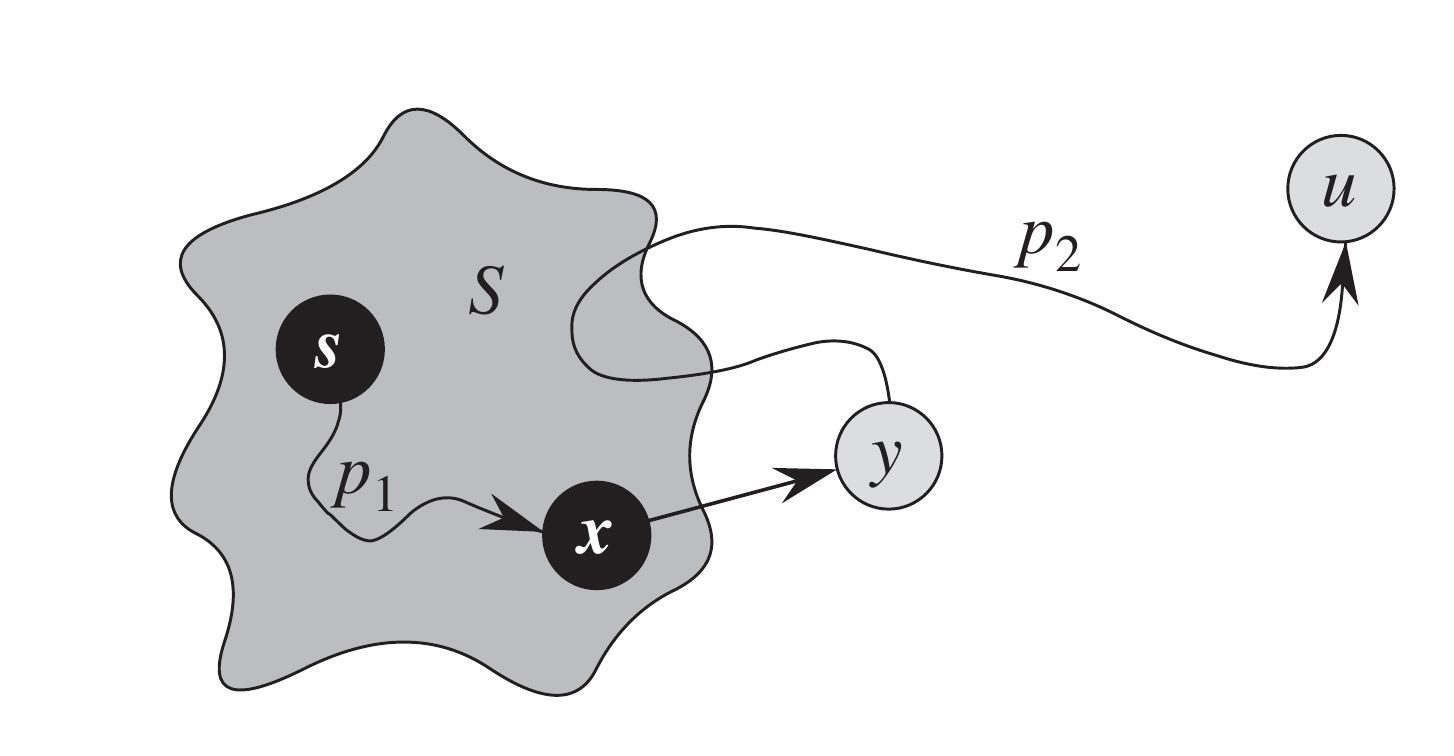
\includegraphics[scale=.2]{res/dijkstra}
	\captionof{figure}{}\label{fig:dijkstra}
\end{center}

Asseriamo che $d[y] = \delta(s,y)$ quando $u$ viene aggiunto a $S$. Per dimostrare ciò, osserviamo che $x \in S$. Allora, poiché $u$ è stato scelto come il primo vertice per il quale $d[u] \neq \delta(s,u)$ quando esso viene aggiunto a $S$, era vero che $d[x]=\delta(s,x)$ quando $x$ è stato aggiunto a $S$. L'arco $(x,y)$ è stato rilassato in quell'istante, quindi l'asserzione è dimostrata per il Lemma 5.

Adesso possiamo ottenere una contraddizione per dimostrare che $d[u]= \delta(s,u)$. Poiché $y$ precede $u$ in un cammino minimo da $s$ a $u$ e tutti i pesi degli archi non sono negativi, si ha $\delta(s,y) \leq \delta(s,u)$ e quindi:
\begin{align*}
	d[y] &= \delta(s,y) \\
	&= \delta(s,u)\\
	&= d[u]
\end{align*}
Tuttavia, poiché entrambi i vertici $u$ e $y$ si trovavano in $Q$ quando $u$ venne scelto, si ha $d[u] \leq d[y]$. Quindi le due disuguaglianze sono delle uguaglianze:
\begin{displaymath}
	d[y] = \delta(s,y) = \delta(s,u) = d[u]
\end{displaymath}
Di conseguenze $d[u]= \delta(s,u)$, che contraddice la nostra scelta di $u$. Concludiamo quindi che $d[u]=\delta(s,u)$ quando $u$ viene aggiunto a $S$ e che questa uguaglianza permane in tutti gli istanti successivi. 
\end{proof}


\chapter{La crescita delle funzioni}

Il tasso di crescita del tempo di esecuzione di un algoritmo fornisce una semplice caratterizzazione dell'efficienza dell'algoritmo; inoltre, ci consente di confrontare le prestazioni relative di algoritmi alternativi.
Quanto operiamo con dimensioni dell'input abbastanza grandi da rendere rilevante soltanto il tasso di crescita del tempo di esecuzione, stiamo studiando l'efficienza \textbf{asintotica} degli algoritmi. In altre parole, ci interessa sapere come aumenta il tempo di esecuzione di un algoritmo al crescere della dimensione dell'input \textit{al limite}, quando la dimensione dell'input cresce senza limitazioni.

\section{Notazione asintotica}
Le notazioni che usiamo per descrivere il tempo di esecuzione  asintotico di un algoritmo sono definite in termini di funzioni il cui dominio è l'insieme dei numeri naturali $\mathbb{N}=\{0,1,2,3,\ldots\}$.

\subsection{Notazione Theta grande}

\dfn{Notazione Theta grande}{
	Per una data funzione $g(n)$, indichiamo con $\Theta(g(n))$ l'insieme delle funzioni:
	\begin{equation}\label{eq:theta_def}
		\Theta(g(n))= \biggl \{ f(n) \; | \; \exists c_{1},c_{2},n_{0} \in \mathbb{N} \Bigl( \forall n \geq n_{0} \bigl(0 \leq  c_{1}\cdot g(n) \leq f(n) \leq c_{2}\cdot g(n) \;\; \forall \; n \geq n_{0}\bigr) \Bigr) \biggl \}
	\end{equation}
}

Una funzione $f(n)$ appartiene all'insieme $\Theta(g(n))$ se esistono delle costanti positive $c_{1}$ e $c_{2}$ tali che possa essere ``racchiusa'' fra $c_{1}\cdot g(n)$ e $c_{2}\cdot g(n)$, per valori sufficientemente grandi di $n$. Poiché $\Theta (g(n))$ è un insieme, dovremmo scrivere ``$f(n) \in \Theta(g(n))$'' per indicare che la funzione $f(n)$ è un elemento di $\Theta(g(n))$. Invece, con un abuso di notazione, di solito si trova scritto ``$f(n)=\Theta(g(n))$'' per esprimere lo stesso concetto. Un altro modo per definire che $f(n)$ e $g(n)$ sono \textbf{asintoticamente equivalenti} è il seguente:
\begin{equation}\label{eq:theta2}
	f(n)=\Theta(g(n)) \iff \lim_{n \to +\infty} \frac{f(n)}{g(n)}=k > 0
\end{equation}

\begin{figure}[ht!]
	\centering
	\subfloat[\label{fig:notazioniasintotiche1}]{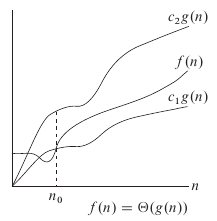
\includegraphics[scale=0.8]{res/Theta.jpg}} \quad
	\subfloat[\label{fig:notazioniasintotiche2}]{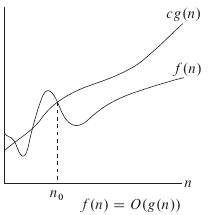
\includegraphics[scale=0.8]{res/Ogrande.jpg}} \quad
	\subfloat[\label{fig:notazioniasintotiche3}]{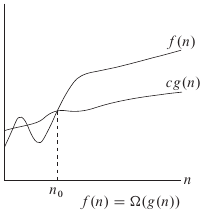
\includegraphics[scale=0.8]{res/Omega.jpg}}
	\caption{Esempi grafici delle notazioni $\Theta$, O grande e $\Omega$}
\end{figure}

La Figura \ref{fig:notazioniasintotiche1} presenta un grafico intuitivo delle funzioni $f(n)$ e $g(n)$, dove $f(n)=\Theta(g(n))$. Per tutti i valori di $n$ a destra di $n_{0}$, il valore di $f(n)$ coincide o sta sopra $c_{1}g(n)$ o sta sotto $c_{2}g(n)$. In altre parole, per ogni $n\geq n_{0}$, la funzione $f(n)$ è uguale a $g(n)$ a meno di un fattore costante. Si dice che $g(n)$ è un \textbf{limite asintoticamente stretto} per $f(n)$.


\begin{example}
		Dimostriamo che $\frac{1}{2}n^{2}-3n = \Theta(n^{2})$.
	Per farlo dobbiamo determinare le costanti positive $c_{1}$, $c_{2}$ e $n_{0}$ in modo che:
	\begin{displaymath}
		c_{1}n^{2} \leq \frac{1}{2}n^{2}-3n \leq c_{2}n^{2}
	\end{displaymath}

	per qualsiasi $n \geq n_{0}$. Dividendo per $n^{2}$, si ha:
	\begin{displaymath}
		c_{1} \leq \frac{1}{2}-\frac{3}{n} \leq c_{2}
	\end{displaymath}

	La disuguaglianza destra può essere resa valida per qualsiasi valore di $n \geq 1$ scegliendo una costante $c_{2}\geq \frac{1}{2}$.

	Analogamente, la disuguaglianza sinistra può essere resa valida per qualsiasi valore di $n \geq 7$ scegliendo una costante $c_{1} \leq \frac{1}{14}$. Quindi scegliendo $c_{1}=\frac{1}{14}$, $c_{2}=\frac{1}{2}$ e $n_{0}=7$, possiamo verificare che $\frac{1}{2}n^{2}-3n = \Theta(n^{2})$.

\end{example}

\subsection{Notazione O grande}
La notazione $\Theta$ limita asintoticamente una funzione da sopra e da sotto. Quando invece abbiamo soltanto un \textbf{limite asintotico superiore}, utilizziamo la notazione O grande.

\dfn{Notazione O grande}{
	Per una data funzione $g(n)$, denotiamo con $O(g(n))$ l'insieme delle funzioni:
	\begin{equation}
		O(g(n))= \biggl \{ f(n)\; | \; \exists  c, n_{0} \in \mathbb{N}  \Bigl( \forall \; n \geq n_{0} \bigl(0 \leq f(n) \leq cg(n) \bigr)  \Bigr) \biggl \}
	\end{equation}
}
La notazione O si usa per assegnare un limite superiore a una funzione, a meno di un fattore costante. Un altro modo per definire che $f(n)$ \textit{non cresce più velocemente} di $g(n)$ è il seguente:
\begin{equation}
	f(n)=O(g(n)) \iff \lim_{n \to +\infty} \frac{f(n)}{g(n)}=0
\end{equation}
La funzione $g(n)$ è quindi un infinito superiore rispetto a $g(n)$. La figura \ref{fig:notazioniasintotiche2} illustra il concetto intuitivo che sta dietro questa notazione. Per qualsiasi valore n a destra di $n_{0}$, il valore della funzione $f(n)$ coincide o sta sotto $cg(n)$.

\begin{osservation}
	Notiamo che $f(n)=\Theta(g(n)) \implies f(n)=O(g(n))$, in quanto la notazione $\Theta$ è una notazione più forte della notazione O. Secondo la notazione degli insiemi possiamo scrivere $\Theta(g(n)) \subseteq O(g(n))$.
\end{osservation}

\subsection{Notazione Omega grande}
Così come la notazione O grande fornisce un limite asintotico \textit{superiore} a una funzione, la notazione $\Omega$ fornisce un \textbf{limite asintotico inferiore}.

\dfn{Notazione Omega grande}{
	Per una data funzione $g(n)$, denotiamo con $\Omega(g(n))$ l'insieme delle funzioni
	\begin{equation}
		\Omega(g(n))= \biggl \{ f(n)\; | \; \exists c,n_{0} \in \mathbb{N} \Bigl( \forall \; n \geq n_{0} \bigl( 0 \leq cg(n) \leq f(n) \;\; \bigr) \Bigr)  \biggr \}
	\end{equation}
}

Un altro modo per dire che $f(n)$ \textit{non cresce più lentamente} di $g(n)$ è attraverso il seguente limite che esprime il fatto che $g(n)$ è un infinito superiore rispetto a $f(n)$:
\begin{equation}
	f(n)=\Omega(g(n)) \iff \lim_{n \to +\infty} \frac{f(n)}{g(n)}= + \infty
\end{equation}

Il concetto intuitivo che sta dietro la notazione $\Omega$ è illustrato nella figura \ref{fig:notazioniasintotiche3}. Per tutti i valori di n a destra di $n_{0}$, il valore di $f(n)$ coincide o sta sopra $cg(n)$.

\subsection{Proprietà delle relazioni asintotiche}
Molte delle proprietà delle relazioni fra numeri reali si applicano anche ai confronti asintotici. Supponiamo che $f(n)$ e $g(n)$ siano asintoticamente positive.

\begin{teorbox}[Proprietà transitiva]
		Valgono le seguenti proprietà:
	\begin{eqnarray}
		f(n)=\Theta(g(n)) \wedge g(n)=\Theta(h(n)) \implies f(n)=\Theta(h(n)) \\
		f(n)=O(g(n)) \wedge g(n)=O(h(n)) \implies f(n)=O(h(n)) \label{eq:O_transitivity}\\
		f(n)=\Omega(g(n)) \wedge g(n)=\Omega(h(n)) \implies f(n)=\Omega(h(n))
	\end{eqnarray}
\end{teorbox}
\begin{proof}
	Dimostriamo per comodità la \ref{eq:O_transitivity}, le altre proprietà si dimostrano in modo analogo. Per definizione di O grande:
	\begin{eqnarray}
		\exists n_{0} > 0 \quad \exists c_{1}>0 \quad \forall n \geq n_{0} \quad f(n)\leq c_{1}g(n) \nonumber \\
		\exists n_{1} > 0 \quad \exists c_{2}>0 \quad \forall n \geq n_{0} \quad g(n)\leq c_{2}h(n) \nonumber
	\end{eqnarray}
	Assumendo queste due formule vere fissiamo $n_{2}=\mbox{max}\{n_{0},n_{1}\}$ quindi
	\begin{displaymath}
		\exists n_{2} > 0 \quad \exists c_{1},c_{2}>0 \quad \forall n \geq n_{2} \quad f(n)\leq cg(n) \quad \wedge \quad g(n) \leq c_{2}h(n)
	\end{displaymath}
	Maggiorando:
	\begin{displaymath}
	f(n) \leq c_{1}c_{2}h(n)
	\end{displaymath}
	Ponendo $\overline{c}=c_{1}c_{2}$ si ottiene
	\begin{displaymath}
		\exists n_{2} > 0 \quad \exists \overline{c}>0 \quad \forall n \geq n_{2} \quad f(n) \leq \overline{c}h(n)
	\end{displaymath}
	Quindi $f(n)=O(h(n))$.
\end{proof}


\begin{teorbox}[Proprietà riflessiva]
		Valgono le seguenti proprietà:
	\begin{eqnarray}
		f(n)=\Theta(f(n)) \\
		f(n)=O(f(n)) \\
		f(n)=\Omega(f(n))
	\end{eqnarray}
\end{teorbox}

\begin{teorbox}[Proprietà simmetrica]
		Vale la seguente proprietà
	\begin{equation}
		f(n)=\Theta(g(n)) \Leftrightarrow g(n)=\Theta(f(n))
	\end{equation}
\end{teorbox}


	Dalla definizione di notazione $\Theta$:
	\begin{equation}
		\exists n_{0}>0 \quad \exists c_{1},c_{2} > 0 \quad c_{1}g(n) \leq f(n) \leq c_{2}g(n)
	\end{equation}
	possiamo estrarre delle costanti utili per dimostrare il teorema, infatti:
	\begin{eqnarray}
		c_{1}g(n) \leq f(n) \leftrightarrow f(n) \leq \frac{1}{c_{1}} f(n) \nonumber \\
		f(n) \leq c_{2}g(n) \leftrightarrow \frac{1}{c_{2}} \leq g(n) \nonumber \\
	\end{eqnarray}
	quindi ponendo
	\begin{eqnarray}
		c_{3}=\frac{1}{c_{1}} \nonumber \\
		c_{4}=\frac{1}{c_{2}} \nonumber
	\end{eqnarray}
	possiamo scrivere
	\begin{equation}
		\exists n_{0}>0 \quad \exists c_{3},c_{4} > 0 \quad c_{4}f(n) \leq g(n) \leq c_{3}f(n)
	\end{equation}
	ovvero $g(n)=\Theta(f(n))$.
\begin{flushright}
	\blacksquare
\end{flushright}

\begin{teorbox}[Simmetria trasposta]
		Vale la seguente proprietà
	\begin{equation}
		f(n)=O(g(n)) \Leftrightarrow g(n)=\Omega(f(n))
	\end{equation}
\end{teorbox}

\section{Ricerca delle costanti mediante metodo grafico}
Attraverso la definizione mediante limite delle notazioni O grande, $\Theta$ e $\Omega$ è possibile ottenere un metodo per la ricerca delle costanti $c_{1}$, $c_{2}$ ed $n_{0}$ senza dover applicare necessariamente la definizione analitica. Infatti, posto $$h(n)=\frac{f(n)}{g(n)}$$ è possibile studiare il grafico della sua funzione per ottenere le costanti ricercate.
Osserviamo infatti che, se $f(n)=\Theta(g(n))$ allora vale
\[
\exists n_{0} \quad \exists c_{1},c_{2}>0 \quad \forall n>n_{0} \quad c_{1}g(n)<f(n)<c_{2}g(n)
\]
dividendo per $g(n)$ si ottiene:
\[
\exists n_{0} \quad \exists c_{1},c_{2}>0 \quad \forall n>n_{0} \quad c_{1}<\frac{f(n)}{g(n)}<c_{2}
\]
e sostituendo il rapporto $\frac{f(n)}{g(n)}=h(n)$ :
\[
\exists n_{0} \quad \exists c_{1},c_{2}>0 \quad \forall n>n_{0} \quad c_{1}<h(n)<c_{2}
\]
Il metodo grafico consiste nella ricerca delle due costanti $c_{1}$ e $c_{2}$ che delimitano l'andamento asintotico della funzione $h(n)$. Supposto quindi che esista e sia limitato il limite
\[
\lim_{n \to +\infty} h(n)= \; l >0
\]
si ottiene che la retta $y=l$ è un asintoto orizzontale per la funzione $h(n)$.

Per tale asintoto possono presentarsi tre situazioni:
\begin{enumerate}
	\item \textbf{$h(n)$ tende a $y=l$ dall'alto.} Scelto un $n_{0}$ in cui la funzione $h(n)$ è \textit{decrescente in un intervallo illimitato} si prendono i valori
	\[
	\begin{cases}
		y=h(n_{0}) \\
		l
	\end{cases}
	\]
	che individuano le due costanti che fanno valere la disuguaglianza $$c_{1}\leq h(n) \leq c_{2}$$
	\item \textbf{$h(n)$ tende a $y=l$ dal basso.} Si procede in maniera analoga al caso precedente, però oltre allo studio della monotonia mediante la derivata prima sarà necessario studiare anche il \textbf{segno della funzione} dato che siamo alla ricerca di \textit{costanti positive}. All'interno della semiretta a destra dove la funzione assume segno positivo si può scegliere a piacere un punto $x_{t}$ e valutare la funzione in quel punto: $y_{1}=h(x_{t})$. Quindi l'insieme delle costanti $(y_{1},l)$ rappresenta una coppia di costanti che garantiscono la proprietà da dimostrare.
	\item \textbf{$h(n)$ tende a $y=l$ in modo oscillante.} In questo caso, poco frequente, $n_{0}$ si deve trovare nell'intervallo in cui l'oscillazione si smorza. All'interno di questo intervallo andiamo a selezionare i valori di minimo e massimo locale.
	
\end{enumerate}
	\begin{figure}[ht!]
		\centering
	\subfloat[Caso 1: $h(n)$ tende al limite dall'alto]{\includegraphics[scale=0.8]{res/asintoto_orizzontale2}}\qquad
	\subfloat[Caso 2: $h(n)$ tende al limite dal basso]{\includegraphics[scale=0.8]{res/asintoto_orizzontale1}}\qquad
	\subfloat[Caso 3: $h(n)$ tende al limite in modo oscillante]{\includegraphics[scale=.8]{res/asintoto_orizzontale3}}
	\caption{}
\end{figure}

\begin{example}
	Siano
	\[
	\begin{array}{l}
		f(n)=n \\
		g(n)=4n-10
	\end{array}
	\]
	Dimostriamo attraverso il metodo grafico che vale $$g(n)=\Theta(f(n))$$

	Si calcola innanzitutto il limite
	\begin{equation}\label{limit1}
		\lim_{n \to \infty} \frac{4n-10}{n}= 4
	\end{equation}


	Esiste quindi un asintoto orizzontale di equazione $y=4$. Siamo interessati alla ricerca delle due costanti che verificano la condizione:
	\begin{equation}\label{disuguaglianza1}
		\exists n_{0} >0 \quad \exists c_{1},c_{2}>0 \quad c_{1}n \leq 4n-10 \leq c_{2}n \quad \forall n > n_{0}
	\end{equation}

	Studiamo quindi la monotonia della funzione $h(n)=\frac{4n-10}{n}$:
	$$
	h'(n)= \frac{10}{n^{2}} > 0 \quad \forall n>0
	$$
	La funzione quindi è strettamente crescente in tutto l'intervallo $(0,+\infty)$
	Per cercare due costanti positive è necessario che la funzione $h(n)$ sia positiva
	$$
	h(n)=\frac{4n-10}{n}>0 \quad \iff \quad n> \frac{5}{2}
	$$
	Prendendo a piacere un $n_{0}$ all'interno dell'intervallo $(\frac{5}{2}, +\infty)$ si troveranno quindi due costanti $c_{1}$ e $c_{2}$ che verificano la disuguaglianza \ref{disuguaglianza1}. Infatti, preso $n_{0}=3$ si valuta la funzione $h(n)$ in quel punto ottenendo $$h(3)=\frac{4\cdot3-10}{3}=\frac{2}{3}$$ mentre la costante $c_{2}$ era stata data dal limite \ref{limit1}.
\end{example}
% Chapter 5: Notazione asintotica
% Chapter 4: Traduzione da ricorsione a iterazione
% Chapter 6: Alberi di ricorsione
% Chapter 8: Algoritmi di ordinamento
\chapter{Algoritmi di ordinamento}\label{cap:ordinamento}
\section{Il problema dell'ordinamento}

\dfn{Ordinamento}{
	Sia $A$ una sequenza di n numeri $\langle a_{1},a_{2},...,a_{n}\rangle$ con $a_{i}\in \mathbb{Z} \quad \forall \; 1 \leq i \leq n$. \textbf{Ordinare} $A$ significa trovare una sequenza $A'$ chiamata \textbf{permutazione ordinata} di $A$, ovvero un riarrangiamento $\langle a'_{1}, a'_{2},...,a'_{n}\rangle$ tale che
	\begin{equation}\label{condizioneordinamento}
		a'_{1}\leq a'_{2} \leq \cdots \leq a'_{n}
	\end{equation}
}

Per ordinare una sequenza si può pensare di generare tutte le permutazioni possibili a partire da tale sequenza e verificare la proprietà di ordinamento \ref{condizioneordinamento}. Da questa idea possiamo dire con certezza che almeno un algoritmo che risolva il problema dell'ordinamento esista dato che, essendo l'ordinamento totale esisterà sicuramente una soluzione. Ovviamente questo approccio è tanto banale quanto complesso. Algoritmi di questo tipo vengono chiamati \textbf{algoritmi di forza bruta (brute force)}.

Nel caso del problema della massima sottosequenza contigua visto in \ref{sottosequenzecontigue}, l'algoritmo di forza bruta aveva un costo quadratico. In questo caso invece, la differenza è abissale. Data una sequenza di $n$ elementi il numero di permutazioni sarà $n!$, controllare la condizione \ref{condizioneordinamento} implica scorrere ogni elemento di ciascuna permutazione raggiungendo così il costo di $\Omega(n \cdot n!)$ che è molto ma molto grande rispetto ad $n^{2}$.

Nel corso di questo capitolo si vedrà che esistono algoritmi più ``sensati'' per la ricerca di una sequenza ordinata. Il problema da porsi sarà quello della loro \textit{costruzione}. Tutti gli algoritmi che si vedranno in questo capitolo avranno un tempo limitato superiormente da $n^{2}$, quindi sarà: $T(n)=O(n^{2})$.  L'idea alla base sarà quella di ordinare mediante l'utilizzo del \emph{confronto}, volta per volta, di coppie di elementi. Chiaramente, nel migliore dei casi il costo sarà lineare (meno di così non sarà possibile scendere). Questa analisi ci permette quindi di limitare l'intervallo all'interno del quale selezionare algoritmi  che siano ``sensati''.

\section{Insertion Sort}
L'algoritmo \textbf{Insertion sort} è un buon metodo per ordinare un piccolo numero di elementi. La sua idea basilare è molto banale ed è simile al modo in cui molte persone ordinano le carte: preso un mazzo di carte, si inseriscono le carte nella loro posizione corretta una dopo l'altra dopo averle confrontate con quelle precedentemente ordinate. In ogni momento quindi, l'algoritmo vede la sequenza divisa in due parti: una ordinata e una disordinata. Consideriamo quindi una sequenza $A$, l'algoritmo \textsc{Insertion Sort} (Algoritmo \ref{alg:insertsort}) ordina i numeri di input \textbf{in place}, nel  senso che i numeri sono risistemati all'interno dell'array $A$ senza l'utilizzo di alcuna struttura ausiliaria. Quando la procedura è completata, l'array di input $A$ contiene la sequenza di output ordinata.

\begin{lstlisting}[caption={\textsc{InsertionSort}(A,n)},language=asd,label=alg:insertsort]
for j=2 to n do
	elem = A[j]
	// Inserisce A[j] nella sequenza ordinata A[1,...,j-1]
	i = j-1
	while i @$\geq$@ 1 && elem < A[i] do
		A[i+1] = A[i]
		i = i-1
	A[i+1] = elem
\end{lstlisting}

\begin{center}
	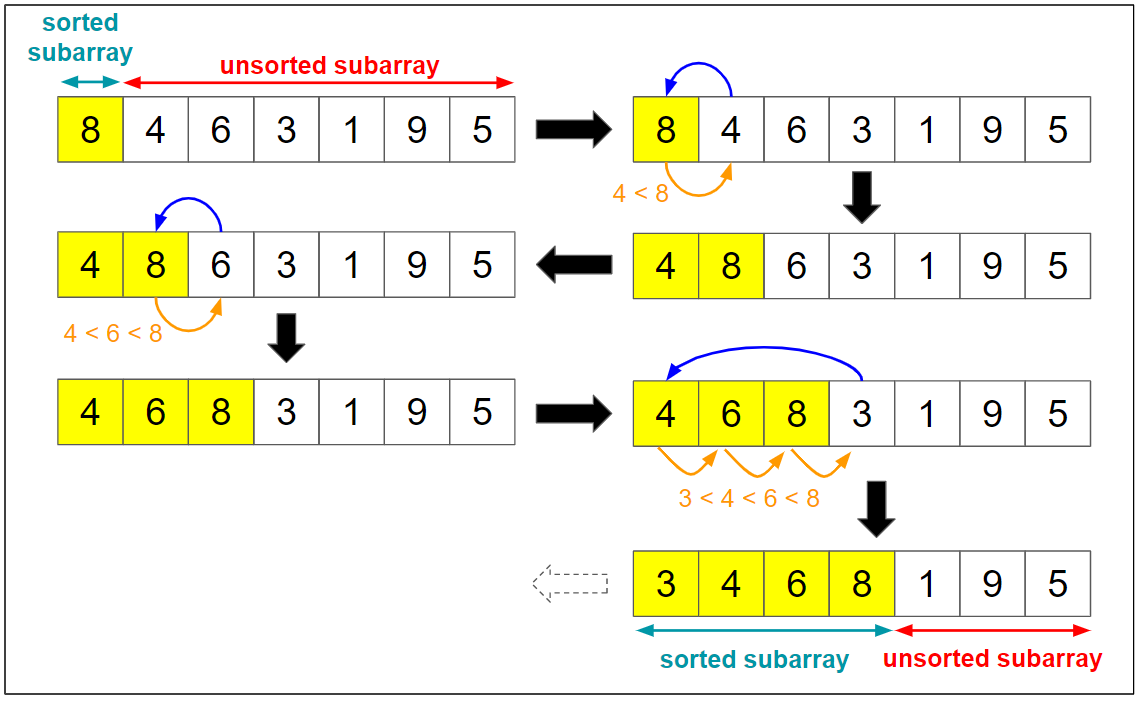
\includegraphics[scale=.3]{res/InsertionSort1}
	\captionof{figure}{Esempio di applicazione di \textsc{Insertion Sort}}
\end{center}

\subsection{Invarianti di ciclo e correttezza di \textsc{InsertionSort}}
Il tempo richiesto dalla procedura \textsc{Insertion-Sort} dipende dall'input: occorre più tempo per ordinare un migliaio di numeri che tre numeri. Inoltre, \textsc{Insertion-Sort} può richiedere quantità di tempo differenti per ordinare due sequenze di input della stessa dimensione a seconda della \textit{qualità} della sequenza. Infatti non si può dire a priori il numero di esecuzioni del ciclo \texttt{while} al rigo 5 dell'Algoritmo \ref{alg:insertsort}.

In casi come questi si andranno a fare due analisi distinte e separate, una prima per quelle classi di istanze ``buone'' che offriranno tempi di esecuzioni brevi e una seconda analisi per quelle istanze dette anche ``peggiori''. Bisogna capire però come \textit{formalizzare la dipendenza dalla bontà dell'input del tempo}. Per rispondere a questa domanda si introducono una serie di parametri, detti $t_{j}$, che indicano il numero di iterazioni della testa del ciclo \texttt{while}, \textit{fissato} l'indice $j$.

Poiché abbiamo che $j$ varia da $2$ a $n$ avremo rispettivamente: $t_{2},...,t_{n}$. Complessivamente la testa del \texttt{while} sarà eseguita quindi $\sum_{j=2}^{n}t_{j}$ volte. Una volta introdotti questi parametri possiamo dire quindi che le istruzioni 6 e 7 saranno eseguite rispettivamente $\sum_{j=2}^{n}(t_{j}-1)$ volte. Si ha così un \textbf{prospetto parametrico} del costo istruzione per istruzione.

\begin{center}
	\begin{tblr}{hlines,vlines,cells={mode=math},row{1}={primary!80!white},column{1}={primary!80!white}}
	\textbf{Istruzione} & \textbf{\# Operazioni} & \textbf{Esecuzioni} \\
	1 & 2 & n \\
	2 & 2 & n-1 \\
	3 & 2 & n-1 \\
	5 & 4 & \sum_{j=2}^{n} t_{j}\\
	6 & 3 & \sum_{j=2}^{n} t_{j-1}\\
	7 & 1 & \sum_{j=2}^{n} t_{j-1}\\
	8 & 2 & n-1\\
\end{tblr}
\end{center}

Il tempo di esecuzione dell'algoritmo è la somma dei tempi di esecuzione per ogni istruzione eseguita.

Per calcolare $T(n)$ sommiamo i prodotti delle colonne \textbf{Numero operazioni} e \textbf{Numero di volte}:
\begin{eqnarray}\label{eq:FormaGenericaInsertSort}
	T(n) &=& 2n+2(n-1)+2(n-1)+4\sum_{j=2}^{n}t_{j}+3\sum_{j=2}^{n}(t_{j}-1)+\sum_{j=2}^{n}(t_{j}-1)\nonumber \\
	&=& 9n-7+4\sum_{j=2}^{n}t_{j}+4\sum_{j=2}^{n}(t_{j}-1)
\end{eqnarray}
L'equazione \ref{eq:FormaGenericaInsertSort} non è una espressione precisa poiché dipendente dai parametri $t_{j}$ però a partire da questa formula possiamo iniziare a fare le due analisi distinte, una per il \textbf{caso peggiore} e una per il \textbf{caso migliore}.
\subsubsection{Caso peggiore}
Nel caso peggiore, ovvero quello di una sequenza ordinata in senso inverso, nella testa del \texttt{while} la condizione $elem<A[i]$ è sempre vera, quindi la condizione farà sempre entrare nel \texttt{while} e il ciclo dipenderà unicamente dall'indice $i\geq 1$. L'algoritmo dovrà confrontare ogni elemento $A[j]$ con ogni elemento dell'intera sottosequenza ordinata $A[1..j-1]$ e quindi sarà $t_{j}=j$ per $j=2,3,...,n$.

Sarà quindi:
\begin{eqnarray}
	T(n) &=& 9n-7+4\sum_{j=2}^{n}j+4\sum_{j=2}^{n}(j-1) \nonumber \\
	&=& 9n -7 + 4\cdot \bigl( \frac{n(n+1)}{2} -1\bigl) +4 \cdot \frac{n(n-1)}{2} \nonumber \\
	&=& 9n -7 + 4 \cdot ((n^{2}+n)-2)+4 \cdot \frac{n(n-1)}{2} \nonumber \\
	&=& 9n - 7 + 4n^{2}+ 4n -8 +2n^{2}-2n \nonumber \\
	&=& 6n^{2}+11n-15
\end{eqnarray}
Possiamo concludere quindi che, nel caso peggiore $T(n)=O(n^{2})$.

\subsubsection{Caso migliore}
In \textsc{Insertion-Sort} il caso migliore si verifica se l'array è già ordinato. Per ogni $j=2,3,...,n$, troviamo che $A[i]<elem$ nella testa del ciclo \texttt{while}, quando $i$ ha il suo valore iniziale $j-1$. Quindi $t_{j}=1$ per $j=2,...,n$ e il tempo di esecuzione nel caso migliore è:
\begin{eqnarray}
	T(n) &=& 9n-7+4\sum_{j=2}^{n}t_{j}+4\sum_{j=2}^{n}(t_{j}-1) \nonumber \\
	&=& 9n-7+4 \sum_{j=2}^{n}1+4\sum_{j=2}^{n}(0) \nonumber \\
	&=& 9n-7+n-1 \nonumber \\
	&=& 10n -8
\end{eqnarray}
Nel caso migliore quindi $T(n)=O(n)$.

\subsubsection{Caso medio}
L'equazione \ref{eq:FormaGenericaInsertSort} ci aveva dato una formula generale, dipendente dai parametri $t{j}$, del costo di \textsc{Insertion-Sort}. Ci si può chiedere però se, fissato l'indice $j$, possa esistere un parametro $t_{medio}$. Nulla vieta di calcolare $t_{medio}$ come la media aritmetica dei vari parametri, assumendo una equiprobabilità delle tipologie di input:
\begin{displaymath}
	t_{medio}=\frac{\sum_{k=1}^{j}k}{j}=\frac{\frac{j(j+1)}{2}}{j}=\Bigl \lfloor \frac{j+1}{2}\Bigl \rfloor
\end{displaymath}
E così la \ref{eq:FormaGenericaInsertSort} diventa:
\begin{eqnarray}
	T_{medio}(n)&=& 9n-7+4\sum_{j=2}^{n}\frac{j+1}{2}+4\sum_{j=2}^{n}\bigl(\frac{j+1}{2}-1\bigl)\nonumber \\
	&=& 9n-7+2\sum_{j=2}^{n}(j+1)+2\sum_{j=2}^{n}(j-1)\nonumber \\
	&=& 9n-7+2\sum_{j=2}^{n}(j+1)+2\sum_{j=1}^{n-1}j \nonumber\\
	&=& 9n-7+2\sum_{j=2}^{n}(j+1)+\frac{n(n-1)}{2}
\end{eqnarray}
Possiamo dire quindi che anche nel caso medio \textsc{Insertion-Sort} ha un comportamento quadratico: $T_{medio}(n)=O(n^{2})$.

\section{Merge Sort}
Per \textsc{Insertion Sort} abbiamo usato un approccio \textbf{incrementale}: dopo avere ordinato il sottoarray $A[1..j-1]$, abbiamo inserito un singolo elemento $A[j]$ nella posizione appropriata, ottenendo il sottoarray ordinato $A[1,...,j]$. L'algoritmo \textsc{Merge-Sort} è un tipo di algoritmo come quelli visti nel Capitolo \ref{cap:ricorrenze}, ovvero un algoritmo ricorsivo. La ricorsione, in questo caso, ridurrà di molto il tempo di esecuzione rispetto ad \textsc{Insertion-Sort} nel caso peggiore.


L'algoritmo \textsc{MergeSort} è conforme al paradigma divide et impera. Esso opera nel modo seguente:
\begin{itemize}
	\item \textbf{Divide:} divide la sequenza degli $n$ elementi da ordinare in due sottosequenze di $n/2$ elementi ciascuna.
	\item \textbf{Impera:} ordina le due sottosequenze in modo ricorsivo utilizzando l'algoritmo merge sort.
	\item \textbf{Combina:} fonde le due sottosequenze ordinate per generare la sequenza ordinata.
\end{itemize}

La ricorsione tocca il fondo quando la sequenza da ordinare ha lunghezza 1, in quel caso non c'è nulla da fare, in quanto ogni sequenza di lunghezza 1 è già ordinata.
\begin{lstlisting}[caption={\textsc{MergeSort}(A,p,r)},language=asd,label=alg:mergesort]
	// Verifica dell'intervallo
	if p<r then
		q = @$\lfloor$@ p+r / 2 @$\rfloor$@
		MergeSort(A,p,q)
		MergeSort(A,q+1,r)
		Merge(A,p,q,r)
\end{lstlisting}


L'operazione chiave dell'algoritmo \textsc{Merge Sort} è la \textit{fusione} di due sottosequenze ordinate nel passo ``combina''. Per effettuare la fusione, utilizziamo una procedura ausiliaria chiamata \textsc{Merge}$(A,p,q,r)$, dove $A$ è un array e $p$, $q$, $r$ sono indici dell'array tali che $p \leq q \leq r$. La procedura assume che i sottoarray $A[p..q]$ e $A[q+1...r]$ siano ordinati; li \textbf{fonde} per formare un unico array ordinato che sostituisce il sottoarray corrente $A[p..r]$.

\subsection{Correttezza dell'algoritmo}
Poiché $p$ ed $r$ indicano l'indice iniziale e finale della sequenza $A$ possiamo dire che $A$ ha $r-p+1$ elementi. Affinché \textsc{Merge-Sort} funzioni bisogna garantire la convergenza del passo ``divide'', ovvero:
\begin{displaymath}
	r-p+1>\underbrace{q-p+1}_{1^{a} sottosequenza} \wedge \underbrace{r-p+1}_{2^{a} sottosequenza} > \underbrace{r-q}_{r-(q+1)+1}
\end{displaymath}

dove $$q=\bigl \lfloor \frac{p+r}{2}\bigl \rfloor$$
e sappiamo che $$\bigl \lfloor\frac{p+r}{2}\bigl \rfloor \leq \frac{p+r}{2}$$
ma allora risulta:
\begin{displaymath}
	r-p+1 > \frac{p+r}{2}-p+1 \implies 2r>p+r \implies r>p
\end{displaymath}
ed essendo la nostra ipotesi proprio $p<r$ abbiamo dimostrato la prima implicazione. Analogamente si procede per la seconda:
\begin{displaymath}
	r-p+1>r-\frac{p+r}{2} \implies -p > -\bigl ( \frac{p+r}{2}+1 \bigl) \implies 2p<p+r+2 \implies p<r+2
\end{displaymath}

Resta solo da dimostrare che, per qualsiasi input, l'algoritmo faccia un numero finito di chiamate ricorsive e che quindi, prima o poi, raggiungerà il caso base. Quando r è molto vicino a p, ovvero quando $r<p+1$ è evidente che sarà $q=\lfloor (p+r)/2 \rfloor = p$ e quindi entrambe le chiamate ricorsive non verranno effettuate poiché la condizione del blocco condizionale if sarà alla prima chiamata $p<p$ ed alla seconda $p+1<r$ (entrambe ovviamente false).

\subsection{L'algoritmo \textsc{Merge}}
\begin{lstlisting}[caption={\textsc{Merge}(A,p,q,r)},language=asd]
	i=p
	k=p
	j=q+1
	while i <= q && j <= r do
		if A[i] <= A[j] then
			B[k] = A[i]
			i=i+1
		else
			B[k] = A[j]
			j=j+1
		k =k+1
	if i < q then
		j=i
	while k <= r do
		B[k] = A[j]
		j = j+1
		k = k+1
\end{lstlisting}

Il costo di esecuzione di \textsc{Merge} è ovviamente lineare poiché si andranno a fare almeno $n$ scritture in memoria:
\begin{displaymath}
	T_{Merge}=\Theta(n)
\end{displaymath}

\subsection{Analisi del costo di \textsc{Merge Sort}}
Per calcolare il tempo di esecuzione dell'algortimo \textsc{Merge Sort} (Algoritmo \ref{alg:mergesort}) si definisce una funzione di ricorrenza del tipo:
\begin{displaymath}
	T_{MergeSort}(N)=
	\begin{cases}
		\Theta(1) & \mbox{ se } n \leq 1\\
		T_{Merge}(N)+\Theta(1) +2 T_{MergeSort}(N/2) & \mbox{ se } n > 1
	\end{cases}
\end{displaymath}
che, sommando $T_{Merge}(N)+\Theta(1)$, diventa:
\begin{equation}\label{eqric:mergesort}
	T_{MergeSort}(N)=
	\begin{cases}
		\Theta(1) & \mbox{ se } n \leq 1\\
		2 T_{MergeSort}(N/2) + \Theta(N) & \mbox{ se } n > 1
	\end{cases}
\end{equation}
Notiamo che l'equazione \ref{eqric:mergesort} è uguale all'equazione \ref{eqricorrenza1} vista nel Capitolo \ref{cap:ricorrenze}. Possiamo concludere quindi che il costo di esecuzione di \textsc{Merge Sort} è:
\begin{displaymath}
	T_{MergeSort}=\Theta(n \log_{2}N)
\end{displaymath}

\section{Selection Sort}
L'idea che sta alla base dell'algoritmo \textsc{Selection Sort} può essere visto come il duale di quella dell'algoritmo \textsc{Insertion Sort}. Infatti, selezionata una posizione della sequenza si trova successivamente l'elemento da metterci dentro.

Come si vede in Figura \ref{fig:SelectionSort}, se iniziamo dall'ultima posizione, ovvero $N$, allora si dovrà trovare il massimo elemento della sequenza evidenziata in azzurro e poi scambiarlo con quello in posizione $N$ (se avessimo preso l'elemento in prima posizione allora si sarebbe dovuto cercare l'elemento più piccolo). Il procedimento si ripete riducendo di volta in volta la sequenza da ordinare che avrà dimensione $N$ poi $N-1$ fino a quando, arrivati alla posizione $2$, non si sarà ottenuta la sequenza ordinata (infatti alla fine dell'ultima iterazione il minimo già si troverà nella posizione $1$).

\begin{figure}[ht!]
	\centering
	\subfloat[All'inizio l'array non è ordinato, selezioniamo quindi l'ultima cella dove dovrebbe trovarsi il massimo.]
	{
		\begin{tikzpicture}
			%\fill[blue, nearly transparent] (0,0) rectangle (6,-1);
			\fill[red] (6,0) rectangle (7,-1);
			\draw (0,0) grid (7,-1);
			\node at (0.5,0.2) {1};
			\node at (1.5,0.2) {2};
			\node at (2.5,0.2) {...};
			\node at (5.5,0.2) {$n-1$};
			\node at (6.5,0.2) {$n$};
		\end{tikzpicture}
	} \hfil
	\subfloat[Chiamo l'algoritmo \textsc{FindMax} sulla sequenza $1,n-1$: se il massimo si trova nella cella 0, evidenziata in verde, eseguo lo swap con la cella rossa.]
	{
		\begin{tikzpicture}
			\fill[green] (0,0) rectangle (1,-1);
			%\fill[blue, nearly transparent] (1,0) rectangle (6,-1);
			\fill[red] (6,0) rectangle (7,-1);
			\draw (0,0) grid (7,-1);
			\node at (0.5,0.2) {1};
			\node at (1.5,0.2) {2};
			\node at (2.5,0.2) {...};
			\node at (5.5,0.2) {$n-1$};
			\node at (6.5,0.2) {$n$};
		\end{tikzpicture}
		}\\
		\subfloat[A questo punto il massimo si trova in posizione corretta.]
		{
			\begin{tikzpicture}
				\fill[red] (0,0) rectangle (1,-1);
				%\fill[blue, nearly transparent] (1,0) rectangle (6,-1);
				\fill[green] (6,0) rectangle (7,-1);
				\draw (0,0) grid (7,-1);
				\node at (0.5,0.2) {1};
				\node at (1.5,0.2) {2};
				\node at (2.5,0.2) {...};
				\node at (6.5,0.2) {$n$};
			\end{tikzpicture}
		} \hfil
	\subfloat[Riduciamo la sottosequenza e ripetiamo il ragionamento. La parte evidenziata in verde risulta già ordinata mentre resta da ordinare la parte evidenziata in giallo.]
	{
		\begin{tikzpicture}
			\fill[red] (5,0) rectangle (6,-1);
			\fill[yellow] (0,0) rectangle (5,-1);
			\fill[green] (6,0) rectangle (7,-1);
			\draw (0,0) grid (7,-1);
			\node at (0.5,0.2) {1};
			\node at (1.5,0.2) {2};
			\node at (2.5,0.2) {...};
			\node at (5.5,0.2) {$n-1$};
			\node at (6.5,0.2) {$n$};
		\end{tikzpicture}
	}
	\caption{Esempio di applicazione dell'Algoritmo \ref{alg:selectionsort}}\label{fig:SelectionSort}
\end{figure}

\begin{minipage}{.4\textwidth}
	\begin{lstlisting}[caption={\textsc{SelectionSort}(A,n)},language=asd,label=alg:selectionsort]
		for i =n to 2 do
			j = FindMax(A,i)
			Swap(A,i,j)
	\end{lstlisting}
\end{minipage}
\begin{minipage}{.4\textwidth}
	\begin{lstlisting}[caption={\textsc{FindMax}(A,n)},language=asd,label=alg:findmax]
		max = i
		for i = 2 to n
		if A[max] < A[i] then
			max = i
		return max
	\end{lstlisting}
\end{minipage}

\subsection{Analisi del costo di \textsc{SelectionSort}}
Poiché sappiamo che la scelta del massimo non può essere fatta con un algoritmo meno che lineare (poiché bisogna confrontare comunque ogni elemento della successione) sembrerebbe che questa sia una soluzione ottimale. Questo algoritmo però è un esempio di come usare usare soluzioni ottime per dei sottoproblemi non rende l'algoritmo ottimale. Ma ciò non significa che l'idea alla base sia pessima; infatti nella sezione \ref{sez:HeapSort} vedremo come abbassare il tempo di esecuzione ad un $\Theta(n \log_{2}n)$.

Si ha quindi:
\begin{eqnarray}
	T_{SS}(N) &=& \Theta(N)+\sum_{i=2}^{N} T_{FindMax}(i)+ \Theta(1) \nonumber \\
	&=& \Theta(N)+ \Theta \Bigl(\sum_{i=2}^{N} i \Bigr) \nonumber \\
	&=& \Theta(N) + \Theta \Biggl( \Bigl(\sum_{i=1}^{N}i \Bigr) -1 \Biggr) \nonumber \\
	&=& \Theta(N) + \Theta \bigl(\frac{n(n+1)}{2} -1\bigr) \nonumber \\
	&=& \Theta(n^{2})
\end{eqnarray}

\section{Heap Sort}\label{sez:HeapSort}
L'algoritmo \textsc{SelectionSort} (Algoritmo \ref{alg:selectionsort}) si è dimostrato essere il peggior algoritmo visto fino a questo momento. Il suo problema non è legato all'idea che sta alla sua base quando piuttosto alla sua \textit{implementazione}. Il punto è che l'algoritmo \textsc{FindMax} (Algoritmo \ref{alg:findmax}) \textbf{non conserva informazioni sull'ordinamento parziale}. L'algoritmo \textsc{HeapSort} cerca di risolvere questa problematica introducendo una struttura dati detta \textbf{heap} (mucchio), per gestire la conservazione di queste informazioni e \textit{ridurre il numero di confronti per la ricerca del massimo}.

\subsection{Gli alberi heap}
Dalle proprietà degli alberi binari pieni\footnote{Vedi \ref{alberi_binari_prop}} si ha che:
\begin{eqnarray}
	N_{\mbox{{\footnotesize nodi interni}}}&=& \sum_{i=0}^{h-1} 2^{i}= 2^{h}-1\\
	h&=&\lfloor \log_{2}n\rfloor \label{altezzaheap} \\
	N_{\mbox{{\footnotesize nodi}}}&=& 2^{h+1}-1 \label{eq:noditree}
\end{eqnarray}
da cui si evince che non tutti gli insiemi possono essere rappresentati da un albero binario pieno (ad esempio un insieme con 5 elementi).

Per garantire che insiemi di ogni cardinalità possano essere rappresentati da un albero heap si usano gli \textbf{alberi binari completi}, ovvero un albero sul quale si impone un rilassamento dei vincoli degli alberi binari pieni. In particolare:
\begin{itemize}
	\item Tutte le foglie sono a livello $h$ oppure $h-1$;
	\item Tutti i nodi interni hanno grado 2 tranne al più un nodo.
\end{itemize}

\dfn{Albero heap}{
	Un \textbf{albero heap} è un albero binario di altezza $h$ tale che, per ogni nodo $i$:
	\begin{enumerate}
		\item tutte le foglie hanno profondità $h$ o $h-1$;
		\item tutti i nodi interni hanno grado $2$, eccetto al più uno;
		\item entrambi i nodi $j$ e $k$ figli di $i$ sono \emph{non maggiori} di $i$.
	\end{enumerate}
}


\begin{osservation}
	Le prime due condizioni definiscono la forma dell'albero, in particolare un albero completo  mentre la terza condizione definisce l'\textbf{architettura} dell'albero. In definitiva, un albero heap è un albero binario completo tale che per ogni nodo entrambi i figli non sono maggiori del padre (proprietà di ordinamento parziale). 
\end{osservation}

\begin{center}
	\begin{tikzpicture}
		[every node/.style={circle,draw,fill=blue!25!white,minimum size=0.5cm},
		level/.style={sibling distance=60mm/#1}]
		\node{45}
		child{
			node{34}
			child{
				node{30}
				child{node{14}}
				child{node{21}}
			}
			child{
				node{25}
				child{node{15}}
				child{node{16}}
			}
		}
		child{
			node{28}
			child{
				node{22}
				child{node{20}}
				child{node{23}}
			}
			child{
				node{12}
				child{node{10}}
				child[missing]
			}
		};
	\end{tikzpicture}
	\captionof{figure}{Esempio di albero heap}\label{fig:heap}
\end{center}

\subsection{Il problema della rappresentabilità}
Dato un qualsiasi $n \in \mathbb{N}$, siamo sicuri che tutti gli insiemi possono essere rappresentati da un albero binario completo? In generale infatti possiamo saltare da alberi pieni contenenti $2^{h+1}-1$ nodi ad alberi con $2^{(h+1)+1}-1=2^{h+2}-1$ nodi. Non esiste però nessun albero pieno con un numero di nodi compreso tra $2^{h+1}-1$ e $2^{h+2}-1$. Se si riuscisse a dimostrare che si possono costruire alberi binari completi a partire da $2^{h+1}-1$ nodi allora si potrebbe garantire la proprietà ricercata.

Sia $h=1$ Allora è possibile considerare due alberi pieni contenenti:
\begin{displaymath}
	2^{h+1}-1 = 2^{1+1}-1=2^{2}-1=4-1=3
\end{displaymath}
e
\begin{displaymath}
	2^{h+2}-1 = 2^{1+2}-1=2^{3}-1=8-1=7
\end{displaymath}
nodi ciascuno come mostrato in figura:

\begin{center}
\begin{minipage}{.45\textwidth}
	\centering
	\begin{tikzpicture}
	[every node/.style={circle,draw,fill=blue!25!white,minimum size=0.5cm}]
	\node{}
	child{
		node{}
	}
	child{
		node{}	
	};
\end{tikzpicture}
\end{minipage}
\hfil
\begin{minipage}{.45\textwidth}
	\centering
	\begin{tikzpicture}
		[every node/.style={circle,draw,fill=blue!25!white,minimum size=0.5cm},
		level/.style={sibling distance=20mm/#1}]
		\node{}
		child{
			node{}
			child{
				node{}
			}
			child{
				node{}	
			}
		}
		child{
			node{}
			child{
				node{}
			}
			child{
				node{}
			}
		};
	\end{tikzpicture}
\end{minipage}
\end{center}

Ad esempio, aggiungendo un nodo all'albero pieno con tre nodi si ottiene un albero completo avente 4 nodi compreso tra i due alberi pieni. Procedendo induttivamente con questa estensione possiamo dire quindi che il problema della cardinalità è stato risolto: dall'arbitrarietà di $h$ possiamo costruire alberi completi per ogni numero di nodi $x$ tali che:
\begin{displaymath}
	2^{h+1}-1 \leq x \leq 2^{h+2}-1
\end{displaymath}

Il rilassamento che abbiamo fatto garantisce la proprietà \ref{altezzaheap}? Bisogna dimostrare cioè che anche per un albero completo vale la proprietà di essere \textit{il più corto con quel numero di nodi} e che quindi è possibile ancora scrivere l'altezza in corrispondenza del numero di nodi. Chiaramente, negli alberi completi non vale più la proprietà  \ref{eq:noditree} poiché abbiamo dimostrato che un albero completo \textbf{può avere un numero di nodi qualsiasi}. Ma è vero anche che $2^{h}\leq n \leq 2^{h+1}$ e quindi $n$ o è una potenza di due o si trova tra due potenze di due.

Dunque, sapendo che $\forall n \in \mathbb{N}, \exists h \geq 0$
\begin{displaymath}
	2^{h}-1 \leq n \leq 2^{h+1}-1 \Rightarrow 2^{h+1}-1 \leq n \leq 2^{h+2}-1
\end{displaymath}
applicando il logaritmo a tutti i membri:
\begin{displaymath}
	\log(2^{h+1}-1) \leq \log n \leq \log(2^{h+1}-1) \Rightarrow \lfloor \log(2^{h+1}-1)\rfloor \leq {\lfloor \log n \rfloor} \leq {\lfloor \log(2^{h+2}-1) \rfloor}
\end{displaymath}
Quindi $h \leq \lfloor \log n \rfloor \leq h+1$, ed essendo $\lfloor \log n \rfloor$ un intero si ha $\lfloor \log n \rfloor = h$. Dunque, anche gli alberi completi ottimizzano l'altezza per il numero di nodi.

\subsection{Implementazione degli alberi heap}
L'albero heap è una \textbf{struttura dati astratta}, bisogna quindi porsi il problema di come implementarla attraverso una \textbf{struttura dati concreta}. In particolare, uno heap può essere implementato:
\begin{itemize}
	\item come un albero a puntatori;
	\item come un array.
\end{itemize}

\subsubsection{Da albero ad array}
Come osservato in precedenza, \textbf{qualsiasi sequenza numerica può essere rappresentata in un albero completo} in un modo del tutto naturale ponendo come unica condizione il fatto che i nodi dell'albero siano \textbf{contigui}.

Si consideri ad esempio l'albero heap mostrato in figura \ref{fig:heap}. È possibile rappresentare tale albero mediante un array eseguendo una scansione livello per livello:

\begin{center}
	\begin{tikzpicture}
		[level 1/.style={sibling distance=5cm},
		level 2/.style={sibling distance=3cm},
		level 3/.style={sibling distance=1cm},
		mynode/.style = {shape=circle, draw, align=center, fill=blue!25!white,minimum size=.5cm}]
		\node[mynode,name=1]{45}
		child{
			node[mynode,name=2]{34}
			child{
				node[mynode,name=4]{30}
				child{
					node[mynode,name=8]{14}
				}
				child{
					node[mynode,name=9]{21}
				}
			}
			child{
				node[mynode,name=5]{25}
				child{
					node[mynode,name=10]{15}
				}
				child{
					node[mynode,name=11]{16}
				}
			}
		}
		child{
		node[mynode,name=3]{28}
			child{
				node[mynode,name=6]{22}
				child{
					node[mynode,name=12]{20}
				}
				child[mynode,missing]
			}
			child{
				node[mynode,name=7]{12}
			}
	};
\foreach \i in {1,...,12}
{
	\node[anchor=north] at (\i.south) {\i};
}
	\end{tikzpicture}
\end{center}

Quindi gli indici dell'array andranno da sinistra verso destra livello per livello:
\begin{center}
    \begin{tikzpicture}
	\def\sz{8mm}
	\tikzstyle{block} = [draw, fill=black!10, rectangle,minimum height=\sz, minimum width=\sz ];
	\tikzstyle{plain} = [draw=none,fill=none];
	\def\arr{45,34,28,30,25,22,12,14,21,15,16,20};
	\newcounter{ind};
	\setcounter{ind}{0};
	\node[plain] { $A$ };
	\foreach \item in \arr
	{
		\addtocounter{ind}{1};
		\node[block,name=\item] at (\theind*\sz,0) { \item };
		\node[plain] at (\theind*\sz,0.7) { \theind };
	}
\end{tikzpicture}
\end{center}

 Dunque \textbf{un heap può essere implementato come un array }$A$ in cui:
\begin{itemize}
	\item la radice dello heap sta nella posizione $A[0]$ dell'array.
	\item Se il nodo $i$ dello Heap sta nella posizione $i$ dell'array (cioè $A[i]$) allora:
	\begin{itemize}
		\item il figlio sinistro di $i$ sta nella posizione $2i$;
		\item il figlio destro di $i$ sta nella posizione $2i+1$;
	\end{itemize}
\end{itemize}

Dunque \textbf{un array sarà un albero heap} se soddisfa le condizioni:
\begin{eqnarray}
	 A[i]\geq A[2i]  \label{eq:heap1}\\
	A[i]\geq A[2i+1] \label{eq:heap2}
\end{eqnarray}

Da questa corrispondenza si ottiene anche che le posizioni nell'array che contengono le foglie sono quelle per cui $2i>n$, da cui $i > \frac{n}{2}$, ovvero nella \textbf{seconda metà di destra dell'array}. Più precisamente i nodi interni andranno da $1 \leq i \leq \lfloor n/2 \rfloor$, mentre le foglie da $\lfloor n/2 \rfloor \leq i \leq n$.

Un array $A$ che rappresenta un albero heap è caratterizzato dall'attributo \texttt{\textbf{heapsize}} il quale denota il numero di nodi dell'albero heap correntemente memorizzati nel vettore. Chiaramente si ha sempre:
\begin{displaymath}
	0 \leq \text{\texttt{heapsize}} \leq \text{\texttt{A.lenght}}
\end{displaymath}
Anche se ci possono essere dei numeri memorizzati in tutto l'array $A$, soltanto i numeri $A[1,\ldots,heapsize]$ sono elementi validi dell'heap. La radice dell'albero viene sempre memorizzata in $A[1]$. Se $i$ è l'indice di un nodo, gli indici del padre \textsc{Parent}$(i)$, del figlio sinistro \textsc{Left}$(i)$ e del figlio destro \textsc{Right}$(i)$ possono essere calcolati mediante le seguenti procedure:
\begin{minipage}{.3\textwidth}
	\begin{lstlisting}[caption={\textsc{Parent}(i)},language=asd]
		return  @$\lfloor \frac{n}{2}\rfloor$@
	\end{lstlisting}
\end{minipage}
\hfil
\begin{minipage}{.3\textwidth}
	\begin{lstlisting}[caption={\textsc{Left}(i)},language=asd]
		return @$2i$@
	\end{lstlisting}
\end{minipage}
\hfil
\begin{minipage}{.3\textwidth}
	\begin{lstlisting}[caption={\textsc{Right}(i)},language=asd]
		return @$2i+1$@
	\end{lstlisting}
\end{minipage}

\begin{center}
	\begin{tikzpicture}
		\def\sz{8mm}
		\tikzstyle{block} = [draw, fill=black!10, rectangle,minimum height=\sz, minimum width=\sz ];
		\tikzstyle{plain} = [draw=none,fill=none];
		\def\arr{45,34,28,30,25,22,12,14,21,15,16,20};
		\setcounter{ind}{0};
		\node[plain] { $A$ };
		\foreach \item in \arr
		{
			\addtocounter{ind}{1};
			\node[block,name=\item] at (\theind*\sz,0) { \item };
			\node[plain] at (\theind*\sz,0.7) { \theind};
		}
	\draw[-] (45.south) to [bend right=35] (34.south);
	\draw[-] (45.south) to [bend right=35] (28.south);
	\draw[-] (34.north) to [bend left=35] (30.north);
	\draw[-] (34.north) to [bend left=35] (25.north);
	\draw[-] (28.south) to [bend right=35] (22.south);
	\draw[-] (28.south) to [bend right=35] (12.south);
	\draw[-] (30.north) to [bend left=35] (14.north);
	\draw[-] (30.north) to [bend left=35] (21.north);
	\draw[-] (25.south) to [bend right=35] (15.south);
	\draw[-] (25.south) to [bend right=35] (16.south);
	\draw[-] (22.south) to [bend right=35] (20.south);
	\end{tikzpicture}
\captionof{figure}{}\label{fig:heap3}
\end{center}

\subsection{L'algoritmo \textsc{Heapify}: conservare la proprietà dell'heap}
Come osservato fino a questo punto, un vettore rappresentante un albero heap gode di un ordinamento parziale dato dalle relazioni \ref{eq:heap1} e \ref{eq:heap2}. Basta osservare l'array $A$ mostrato in Figura \ref{fig:heap3} per convincersi del fatto che tale vettore non sia totalmente ordinato.

Volendo ripetere il ragionamento fatto per l'algoritmo \textsc{SelectionSort} (Algoritmo \ref{alg:selectionsort}) si potrebbe pensare di utilizzare un algoritmo \textsc{FindMax} che, dato un array $A$ e un indice $i$, restituisca l'indice $j$ del massimo elemento dell'array $A[i,\ldots,n]$. Tale algoritmo però non è sufficiente per garantire che l'array $A$ sia di nuovo un heap. Infatti, se si considera l'array $A$ mostrato in Figura \ref{fig:heap3} e si applica l'algoritmo \textsc{FindMax}$(A,1)$ si ottiene che il massimo elemento è $45$ e che si trova nella posizione $1$. Se si scambia l'elemento $45$ con l'elemento $20$ si ottiene l'array $A'$ mostrato in Figura \ref{fig:heap4} che non è un heap.

\begin{center}
	\begin{tikzpicture}
		\def\sz{8mm}
		\tikzstyle{block} = [draw, fill=black!10, rectangle,minimum height=\sz, minimum width=\sz ];
		\tikzstyle{plain} = [draw=none,fill=none];
		\def\arr{20,34,28,30,25,22,12,14,21,15,16,45};
		\setcounter{ind}{0};
		\node[plain] { $A'$ };
		\foreach \item in \arr
		{
			\addtocounter{ind}{1};
			\node[block,name=\item] at (\theind*\sz,0) { \item };
			\node[plain] at (\theind*\sz,0.7) { \theind};
		}
	\draw[-] (20.south) to [bend right=35] (34.south);
	\draw[-] (20.south) to [bend right=35] (28.south);
	\draw[-] (34.north) to [bend left=35] (30.north);
	\draw[-] (34.north) to [bend left=35] (25.north);
	\draw[-] (28.south) to [bend right=35] (22.south);
	\draw[-] (28.south) to [bend right=35] (12.south);
	\draw[-] (30.north) to [bend left=35] (14.north);
	\draw[-] (30.north) to [bend left=35] (21.north);
	\draw[-] (25.south) to [bend right=35] (15.south);
	\draw[-] (25.south) to [bend right=35] (16.south);
	\draw[-] (22.south) to [bend right=35] (45.south);
	\end{tikzpicture}
	\captionof{figure}{}\label{fig:heap4}
\end{center}
Per questo motivo, per mantenere la proprietà di heap è necessario usare l'algoritmo \textsc{Heapify} (Algoritmo \ref{alg:heapify}) che, dato un array $A$ e un indice $i$, \textbf{ripristina la proprietà di heap} nell'albero binario con radice in $i$ assumendo che i sottoalberi con radici in \textsc{Left}$(i)$ e \textsc{Right}$(i)$ siano heap e che l'unico elemento che non rispetta la proprietà di heap sia $A[i]$. L'algoritmo \textsc{Heapify} non fa altro che far ``scendere'' l'elemento $A[i]$ nell'albero fino a che l'albero con radice in $i$ non sia un heap.

\begin{example}
	Supponiamo di avere il vettore: $A= [16,4,10,14,7,9,3,2,8,1]$. La Figura \ref{fig:heapify} mostra l'azione dell'algoritmo \textsc{Heapify}.
\end{example}

\begin{center}
	\begin{minipage}{\textwidth}
		\centering
		\begin{tikzpicture}
			[mynode/.style={circle,draw,fill=blue!25!white,minimum size=0.5cm},
			level 1/.style={sibling distance=4cm},
			level 2/.style={sibling distance=3cm},
			level 3/.style={sibling distance=1cm},]
			\node[mynode,name=1]{16}
			child
			{
				node[mynode,name=2,fill=red!25!white]{4}
				child
				{
					node[mynode,name=4]{14}
						child
						{
							node[mynode,name=8]{2}
						}
						child
						{
							node[mynode,name=9]{8}	
						}
				}
					child
					{
						node[mynode,name=5]{7}
							child
							{
								node[mynode,name=10]{1}
							}
							child[missing]
					}
			}
			child
			{
				node[mynode,name=3]{10}
				child
				{
					node[mynode,name=6]{9}
				}
				child
				{
					node[mynode,name=7]{3}
				}
			};
		\foreach \i in {1,...,10}
		{
			\node[anchor=north] at (\i.south) {\i};
		}
		\end{tikzpicture}
	\captionof{figure}{La configurazione iniziale, con $A[2]$ nel nodo $i=2$ che viola le proprietà di heap.}
	\end{minipage}
	\\
	\begin{minipage}{\textwidth}
		\centering
		\begin{tikzpicture}
			[mynode/.style={circle,draw,fill=blue!25!white,minimum size=0.5cm},
			level 1/.style={sibling distance=4cm},
			level 2/.style={sibling distance=3cm},
			level 3/.style={sibling distance=1cm},]
			\node[mynode,name=1]{16}
			child
			{
				node[mynode,name=2]{14}
				child
				{
					node[mynode,name=4,fill=red!25!white]{4}
					child
					{
						node[mynode,name=8]{2}
					}
					child
					{
						node[mynode,name=9]{8}	
					}
				}
				child
				{
					node[mynode,name=5]{7}
					child
					{
						node[mynode,name=10]{1}
					}
					child[missing]
				}
			}
			child
			{
				node[mynode,name=3]{10}
				child
				{
					node[mynode,name=6]{9}
				}
				child
				{
					node[mynode,name=7]{3}
				}
			};
			\foreach \i in {1,...,10}
			{
				\node[anchor=north] at (\i.south) {\i};
			}
		\end{tikzpicture}
	\captionof{figure}{Le proprietà di heap vengono ripristinate nel nodo $2$ scambiando $A[2]$ con $A[4]$; ma questo distrugge la proprietà di heap nel nodo 4, sarà necessario richiamare l'algoritmo \textsc{Heapify}$(A,4)$.}
	\end{minipage}
	\\
	\begin{minipage}{\textwidth}
		\centering
			\begin{tikzpicture}
		[mynode/.style={circle,draw,fill=blue!25!white,minimum size=0.5cm},
		level 1/.style={sibling distance=5cm},
		level 2/.style={sibling distance=3cm},
		level 3/.style={sibling distance=1cm},]
		\node[mynode,name=1]{16}
		child
		{
			node[mynode,name=2]{14}
			child
			{
				node[mynode,name=4]{8}
				child
				{
					node[mynode,name=8]{2}
				}
				child
				{
					node[mynode,name=9,fill=green!25!white]{4}	
				}
			}
			child
			{
				node[mynode,name=5]{7}
				child
				{
					node[mynode,name=10]{1}
				}
				child[missing]
			}
		}
		child
		{
			node[mynode,name=3]{10}
			child
			{
				node[mynode,name=6]{9}
			}
			child
			{
				node[mynode,name=7]{3}
			}
		};
		\foreach \i in {1,...,10}
		{
			\node[anchor=north] at (\i.south) {\i};
		}
	\end{tikzpicture}
		\captionof{figure}{La chiamata ricorsiva \textsc{Heapify}$(A,4)$ scambia $A[4]$ con $A[9]$, il nodo $4$ è sistemato e la chiamata \textsc{Heapify}$(A,9)$ non apporta modifiche in quanto le foglie rispettano sempre la proprietà heap.}\label{fig:heapify}
	\end{minipage}
\end{center}

Ad ogni passo, viene determinato il più grande tra $A[i]$, $A[2i]$ e $A[2i+1]$; il suo indice viene memorizzato nella variabile \texttt{max}. Se $A[i]$ è più grande, allora il sottoalbero con radice nel nodo $i$ è un heap e la procedura termina. Altrimenti, uno dei due figli ha l'elemento più grande e $A[i]$ viene scambiato con $A[max]$; in questo modo, il nodo $i$ e i suoi figli soddisfano la proprietà di heap. Il nodo con indice $max$, però, adesso ha il valore originale $A[i]$ e, quindi, il sottoalbero con radice in $max$ potrebbe violare la proprietà di heap. Di conseguenza, deve essere richiamata ricorsivamente la procedura \textsc{Heapify}$(A,max)$ per quel sottoalbero.

\begin{lstlisting}[language=asd,caption={\textsc{Heapify}(A,i)},label=alg:heapify]
	Sx = Left(i)
	Dx = Right(i)
	if (Sx <= heapsize && A[i]<A[Sx]) then
	max = Sx
	else
	max = i
	if (Dx <= heapsize && A[max] < A[Dx]) then
	max = Dx
	if (max @$\neq$@ i) then
	Swap(A,i,max)
	Heapify(A,max)
\end{lstlisting}

Il tempo di esecuzione di \textsc{Heapify} in un sottoalbero di dimensione $n$  con radice in un nodo $i$ è pari al tempo $\Theta(1)$ per sistemare le relazioni fra gli elementi, più il tempo per eseguire \textsc{Heapify} in un sottoalbero con radice in uno dei figli del nodo $i$. Dunque si può affermare che \textsc{Heapify} ha un tempo di esecuzione pari a:
\begin{equation}T_{Heapify}(n) = O(\log n)\end{equation}

L'algoritmo \ref{alg:heapify} non funziona per sequenze che non siano  heap. Infatti, se così fosse si potrebbe usare \textsc{Heapify} per cercare il massimo di una sequenza in un tempo minore di $\Theta(n)$.

\subsection{Trasformare un array in un heap: l'algoritmo \textsc{Costruisci-Heap}}

È possibile utilizzare l'Algoritmo \textsc{Heapify} dal basso verso l'alto per convertire un array $A[1,\ldots,n]$ in un heap:
\begin{itemize}
	\item  Ovviamente una foglia rispetta sempre le proprietà degli heap,  quindi gli ultimi $\lceil \frac{n}{2} \rceil$ elementi dell'array sono già degli heap. Prendendo i padri delle foglie si può applicare \textsc{Heapify} poiché tutti i loro sottoalberi rispettano la proprietà necessaria.
	\item È sufficiente inserire nello heap solo i primi $\lfloor \frac{n}{2} \rfloor$ elementi, utilizzando \textsc{Heapify} per ripristinare la terza condizione degli heap sul sottoalbero del nuovo elemento.
\end{itemize}

Si ha quindi l'Algoritmo \textsc{Costruisci-Heap} (Algoritmo \ref{alg:costruisciheap}).

\begin{lstlisting}[language=asd,caption={\textsc{Costruisci-Heap}(A,n)},label=alg:costruisciheap]
heapsize = n
for(i= @$\lfloor n/2 \rfloor$@ down to 1 ) do
	Heapify(A,i)
\end{lstlisting}

\begin{example}
	Supponiamo di voler costruire un albero heap a partire dall'array $A=[4,1,3,2,16,9,10,14,8,7]$. La Figura \ref{fig:costruisci-heap} mostra il funzionamento dell'Algoritmo \ref{alg:costruisciheap}.
\end{example}

\begin{center}	
\begin{minipage}{.45\textwidth}
	\centering
		\begin{tikzpicture}
		[mynode/.style={circle,draw,fill=blue!25!white,minimum size=0.5cm},
			level/.style={sibling distance=40mm/#1}]
		\node[mynode,name=1]{4}
		child
		{
			node[mynode,name=2]{1}
			child
			{
				node[mynode,name=4]{2}
				child
				{
					node[mynode,name=8]{14}
				}
				child
				{
					node[mynode,name=9]{8}
				}
			}
			child
			{
				node[mynode,name=5,fill=red!25!white]{16}
				child
				{
					node[mynode,name=10]{7}	
				}
				child[missing]
			}
		}
		child
		{
			node[mynode,name=3]{10}
			child
			{
				node[mynode,name=6]{9}
			}
			child 
			{
				node[mynode,name=7]{3}
			}
		};
	\foreach \i in {1,...,10}
	{
		\node[anchor=north] at (\i.south) {\i};
	}
\end{tikzpicture}
\captionof{figure}{Albero binario rappresentato dall'array $A$, l'indice $i$ punta a $\lfloor 10/2 \rfloor =5 $ prima della chiamata a \textsc{Heapify}$(A,5)$.}
\end{minipage}
\hfil
\begin{minipage}{.45\textwidth}
	\centering
			\begin{tikzpicture}
		[mynode/.style={circle,draw,fill=blue!25!white,minimum size=0.5cm},
		level/.style={sibling distance=40mm/#1}]
		\node[mynode,name=1]{4}
		child
		{
			node[mynode,name=2]{1}
			child
			{
				node[mynode,name=4,fill=red!25!white]{2}
				child
				{
					node[mynode,name=8]{14}
				}
				child
				{
					node[mynode,name=9]{8}
				}
			}
			child
			{
				node[mynode,name=5]{16}
				child
				{
					node[mynode,name=10]{7}	
				}
				child[missing]
			}
		}
		child
		{
			node[mynode,name=3]{10}
			child
			{
				node[mynode,name=6]{9}
			}
			child 
			{
				node[mynode,name=7]{3}
			}
		};
		\foreach \i in {1,...,10}
		{
			\node[anchor=north] at (\i.south) {\i};
		}
	\end{tikzpicture}
\captionof{figure}{Struttura dati risultante dopo \textsc{Heapify}$(A,5)$. L'indice $i$ per l'iterazione successiva fa riferimento al nodo 4.}
\end{minipage}\\
\begin{minipage}{.45\textwidth}
	\centering
		\begin{tikzpicture}
		[mynode/.style={circle,draw,fill=blue!25!white,minimum size=0.5cm},
		level/.style={sibling distance=40mm/#1}]
		\node[mynode,name=1]{4}
		child
		{
			node[mynode,name=2]{1}
			child
			{
				node[mynode,name=4]{14}
				child
				{
					node[mynode,name=8]{2}
				}
				child
				{
					node[mynode,name=9]{8}
				}
			}
			child
			{
				node[mynode,name=5]{16}
				child
				{
					node[mynode,name=10]{7}	
				}
				child[missing]
			}
		}
		child
		{
			node[mynode,name=3,fill=red!25!white]{3}
			child
			{
				node[mynode,name=6]{9}
			}
			child 
			{
				node[mynode,name=7]{10}
			}
		};
		\foreach \i in {1,...,10}
		{
			\node[anchor=north] at (\i.south) {\i};
		}
	\end{tikzpicture}
\end{minipage} \hfil
\begin{minipage}{.45\textwidth}
	\centering
	\begin{tikzpicture}
		[mynode/.style={circle,draw,fill=blue!25!white,minimum size=0.5cm},
		level/.style={sibling distance=40mm/#1}]
		\node[mynode,name=1]{4}
		child
		{
			node[mynode,name=2,fill=red!25!white]{1}
			child
			{
				node[mynode,name=4]{2}
				child
				{
					node[mynode,name=8]{14}
				}
				child
				{
					node[mynode,name=9]{8}
				}
			}
			child
			{
				node[mynode,name=5]{16}
				child
				{
					node[mynode,name=10]{7}	
				}
				child[missing]
			}
		}
		child
		{
			node[mynode,name=3]{10}
			child
			{
				node[mynode,name=6]{9}
			}
			child 
			{
				node[mynode,name=7]{3}
			}
		};
		\foreach \i in {1,...,10}
		{
			\node[anchor=north] at (\i.south) {\i};
		}
	\end{tikzpicture}
\end{minipage}\\
\begin{minipage}{.45\textwidth}
	\centering
	\begin{tikzpicture}
		[mynode/.style={circle,draw,fill=blue!25!white,minimum size=0.5cm},
		level/.style={sibling distance=40mm/#1}]
		\node[mynode,name=1,fill=red!25!white]{4}
		child
		{
			node[mynode,name=2]{16}
			child
			{
				node[mynode,name=4]{14}
				child
				{
					node[mynode,name=8]{2}
				}
				child
				{
					node[mynode,name=9]{8}
				}
			}
			child
			{
				node[mynode,name=5]{7}
				child
				{
					node[mynode,name=10]{1}	
				}
				child[missing]
			}
		}
		child
		{
			node[mynode,name=3]{10}
			child
			{
				node[mynode,name=6]{9}
			}
			child 
			{
				node[mynode,name=7]{3}
			}
		};
		\foreach \i in {1,...,10}
		{
			\node[anchor=north] at (\i.south) {\i};
		}
	\end{tikzpicture}
\end{minipage} \hfil
\begin{minipage}{.45\textwidth}
	\centering
	\begin{tikzpicture}
		[mynode/.style={circle,draw,fill=blue!25!white,minimum size=0.5cm},
		level/.style={sibling distance=40mm/#1}]
		\node[mynode,name=1]{16}
		child
		{
			node[mynode,name=2]{14}
			child
			{
				node[mynode,name=4]{8}
				child
				{
					node[mynode,name=8]{2}
				}
				child
				{
					node[mynode,name=9]{4}
				}
			}
			child
			{
				node[mynode,name=5]{7}
				child
				{
					node[mynode,name=10]{1}	
				}
				child[missing]
			}
		}
		child
		{
			node[mynode,name=3]{10}
			child
			{
				node[mynode,name=6]{9}
			}
			child 
			{
				node[mynode,name=7]{3}
			}
		};
		\foreach \i in {1,...,10}
		{
			\node[anchor=north] at (\i.south) {\i};
		}
	\end{tikzpicture}
\captionof{figure}{Heap finale}
\end{minipage}
\captionof{figure}{}\label{fig:costruisci-heap}
\end{center}

Ogni chiamata di \textsc{Costruisci-Heap} costa un tempo $O(\log n)$ e ci sono $O(n)$ di queste chiamate. Quindi, il tempo di esecuzione sarà $O(n \log n)$. Questo limite superiore, sebbene corretto, non è asintoticamente stretto.

Possiamo ottenere un limite più stretto osservando che il tempo per eseguire \textsc{Heapify} (Algoritmo \ref{alg:heapify}) in un nodo varia con l'altezza del nodo nell'albero, e le altezze della maggior parte dei nodi sono piccole. L'analisi più rigorosa si basa sulla proprietà che un heap di $n$ elementi ha un'altezza $\lfloor n/2 \rfloor$ e, per ogni $h$, al massimo $\lceil n/2^{h+1} \rceil$ nodi di altezza $h$. Il tempo richiesto dalla procedura \textsc{Heapify} quando viene chiamata per un nodo di altezza $h$ è $O(h)$, quindi possiamo dire che il costo totale di \textsc{Costruisci-Heap} è limitato superiormente da:
\begin{displaymath}
	\sum_{h=0}^{\lfloor \log n \rfloor} \lceil \frac{n}{2^{h+1}} \rceil O(h)= O\Bigl(n \sum_{h=0}^{\lfloor \log n \rfloor} \frac{h}{2^{h}} \Bigl)
\end{displaymath}


\begin{propbox}
	Derivando entrambi i lati della serie geometrica infinita e moltiplicando per $x$, si ha, 	per $|x|<1$:
	\begin{equation}\label{sommatoria:integrale}
		\sum_{k=0}^{\infty} kx^{k} = \frac{x}{{(1-x)}^{2}}
	\end{equation}
\end{propbox}

L'ultima sommatoria può essere calcolata ponendo $x=1/2$ nella formula \ref{sommatoria:integrale}:
\begin{displaymath}
	\sum_{h=0}^{\infty} \frac{h}{2^{h}} = \frac{1/2}{(1-1/2)^{2}}=2
\end{displaymath}

Quindi, il tempo di esecuzione di \textsc{Costruisci-Heap} può essere limitato così:
\begin{equation}
	O\Bigl(n \sum_{h=0}^{\lfloor \log n \rfloor} \frac{h}{2^{h}} \Bigl) = O\Bigl(n \sum_{h=0}^{\infty} \frac{h}{2^{h}}\Bigl)=O(n)
\end{equation}

Dunque possiamo costruire un heap da un array non ordinato in tempo lineare.

\subsection{L'algoritmo \textsc{HeapSort}}
Come anticipato, l'algoritmo \textsc{HeapSort} è una variazione di \textsc{SelectionSort} in cui la ricerca dell'elemento massimo è facilitata dal mantenimento della sequenza in uno heap.
L'algoritmo inizia utilizzando \textsc{Costruisci-Heap} per costruire un heap nell'array di input $A[1..n]$, dove $n$ è la lunghezza di $A$.

Poiché l'elemento più grande dell'array è memorizzato nella radice $A[1]$, esso può essere inserito nella sua posizione finale corretta scambiandolo con $A[n]$. Se adesso ``togliamo'' il nodo $n$ dall'heap (diminuendo la variabile \textit{heapsize}), notiamo che i figli della radice restano degli alberi heap, ma la nuova radice potrebbe violare la proprietà dell'heap. Per ripristinare questa proprietà, tuttavia, basta una chiamata di \textsc{Heapify}$(A,1)$ (Algoritmo \ref{alg:heapify}), che lascia un heap in $A[1,..,n-1]$. L'algoritmo \textsc{HeapSort} poi ripete questo processo per il sottoalbero heap di dimensione $n-1$ e così via fino ad un heap di dimensione due.

\begin{lstlisting}[caption={\textsc{HeapSort}(A)},label=alg:heapsort,language=asd]
	Costruisci-Heap(A)
	for (i = n down to 2) do
		Swap(A,1,i)
		heapsize = heapsize -1
		Heapify(A,1)
\end{lstlisting}

La procedura \textsc{HeapSort} (Algoritmo \ref{alg:heapsort}) impiega un tempo $O(n \log n)$, in quanto la chiamata di \textsc{Costruisci-Heap} impiega $O(n)$ e ciascuna delle $n-1$ chiamate di \textsc{Heapify} impiega un tempo $O(n \log n)$.

\section{Quick Sort}
L'Algoritmo\textsc{QuickSort}, come \textsc{MergeSort}, è basato sul paradigma divide et impera. Questi sono i tre passi del processo divide et impera per ordinare un generico sottoarray $A[p..r]$.
\begin{enumerate}
	\item \textbf{Divide:} partizionare l'array $A[p..r]$ in due sottoarray $A[p..q-1]$ e $A[q+1..r]$ (eventualmente vuoti) tali che ogni elemento di $A[p..q-1]$ sia minore o uguale ad $A[q]$ che, a sua volta, è minore o uguale ad ogni elemento di $A[q+1..r]$. Calcolare l'indice $q$ come parte di questa procedura di partizionamento.
	\item \textbf{Impera:} ordinare i due sottoarray $A[p..q-1]$ e $A[q+1..r]$ chiamando ricorsivamente \textsc{QuickSort}.
	\item \textbf{Combina:} poiché i sottoarray sono già ordinati, non occorre alcun lavoro per combinarli: l'intero array $A[p..r]$ è già ordinato.
\end{enumerate}

\begin{lstlisting}[caption={\textsc{QuickSort}(A,p,r)},label={alg:quicksort},language=asd]
		if p<r
			q=Partiziona(A,p,r)
			QuickSort(A,p,q)
			QuickSort(A,q+1,r)
\end{lstlisting}
Per ordinare un intero array $A$ di lunghezza $n$, la chiamata iniziale è \textsc{QuickSort}$(A,1,n)$.

\begin{osservation}
	L'algoritmo \textsc{MergeSort} decompone l'array in maniera aritmetica dividendo a metà iterativamente l'array in sottoarray. Così facendo la decomposizione in sottoprobremi risulta più semplice a discapito della fase fusione che è più complessa. L'algoritmo \textsc{QuickSort} decompone in modo ``intelligente'' (pagando di più in termini computazionali) in modo tale da semplificare la fusione dei sottoarray così ottenuti.
\end{osservation}

L'algoritmo \textsc{QuickSort} (Algoritmo \ref{alg:quicksort}) è corretto se valgono le seguenti proprietà:
\begin{enumerate}
	\item La partizione $A[p..q]$ è strettamente minore della sequenza $A[p..r]$.
	\item La partizione $A[q+1..r]$ è strettamente minore della sequenza $A[p..r]$.
	\item Al termine di \textsc{Partiziona}$(A,p,r)$ deve valere:
	\begin{displaymath}
		\forall \ i \in [p,q] \Bigl( \forall j \in [q+1,r] \bigl( A[i] \leq A[j]\bigr)\Bigr)
	\end{displaymath}
che esprime il fatto che ogni elemento di una sottopartizione sinistra deve essere sempre minore od uguale ad un elemento di una sottopartizione di destra.
\end{enumerate}

Le proprietà 1 e 2 possono essere sintetizzate nella proprietà:
\begin{equation}\label{prop:quicksortpartiziona}
	p \leq q < r
\end{equation}

Se questa proprietà non fosse soddisfatta l'algoritmo non funzionerebbe. Infatti è importante escludere i valori $q=p-1$ e $q=r$ per i seguenti motivi: se $q=p-1$ allora \textsc{QuickSort}$(A,p,p-1)$ starebbe passando una istanza vuota, quindi non farebbe nulla. Il problema nasce con la sequenza a destra che andrà da $p$ ad $r$, andando conseguentemente in loop. In modo analogo si ha per $q=r$.

\subsection{Partizionare l'array: l'algoritmo \textsc{Partiziona}}
L'elemento chiave dell'algoritmo \ref{alg:quicksort} è la procedura \textsc{Partiziona} che riarrangia il sottoarray $A[p..r]$ sul posto. I passi fondamentali nell'algoritmo di partizionamento (Algoritmo \ref{alg:partiziona}) sono:
\begin{enumerate}
	\item Estendere le due partizioni verso l'interno finché non si incontra una coppia non correttamente disposta;
	\item Finché le due partizioni non si sono incrociate ($i \geq j$):
	\begin{enumerate}
		\item Scambiare le coppie non correttamente disposte;
		\item Estendere ancora le due partizioni verso l'interno finché non si trova un'altra coppia non correttamente disposta.
	\end{enumerate}
\end{enumerate}
Quando viene chiamato l'algoritmo siamo certi che valga la condizione $p<r$. L'algoritmo \textsc{Partiziona} seleziona un valore $x \in A$, detto \textbf{pivot} e inserisce nella partizione sinistra gli elementi $a_{i} \leq x$ e nella partizione a destra gli elementi $a_{i}\geq x$ (non possiamo mettere il minore stretto perché l'algoritmo deve funzionare per tutte le istanze). 

\marker{yellow!50}{yellow!20!black}{Nel nostro algoritmo \textbf{il pivot è preso nel primo elemento della sottosequenza} ma, in realtà, è possibile prendere qualsiasi elemento dell'array come pivot, a patto che venga messo in prima posizione successivamente.}

\begin{center}
	\begin{tikzpicture}
		\node[draw,fill=black!10,rectangle,name=1,minimum height=1cm,minimum width=4cm]{Partizione di tutti gli elementi minori o uguali al pivot};
		\node[draw,fill=black!10,rectangle,anchor=west,minimum height=1cm,minimum width=4cm]at(1.east){Partizione di tutti gli elementi maggiori o uguali al pivot};
	\end{tikzpicture}
\end{center}

Per scorrere la sequenza si fa uso di due indici:
\begin{enumerate}
	\item Un indice $i$ che partirà da sinistra per essere incrementato fino a quando non trova un valore $y\geq x$
	\item Un indice $j$ che partendo da destra viene decrementato fino a quando non trova un valore $z \leq x$
\end{enumerate}
Una volta fermati gli indici si effettua uno scambio e si ripete il processo fino a quando gli indici non si incrociano: vale cioè la condizione $i \geq j$.

\begin{lstlisting}[caption={\textsc{Partiziona}(A,p,r)},label=alg:partiziona,language=asd]
	x=A[p]
	j=r+1
	i=p-1
	repeat
		repeat
			j=j-1
		until (A[j] @$\leq$@ x)

		repeat
			i=i+1
		until (A[i]@$\geq$@ x)

		if (i<j)
			Swap(A,i,j)
	until (i	@$\geq$@ j)
	return j
\end{lstlisting}

\begin{example}
	Consideriamo l'array $A=[2,8,7,1,3,5,6,4]$ e osserviamo l'esecuzione dell'algoritmo \textsc{QuickSort}$(A,1,8)$.
\end{example}

La procedura di ordinamento inizia con l'invocazione di \textsc{QuickSort}$(A,1,8)$ il quale chiama \textsc{Partiziona}$(A,1,8)$. Il pivot (evidenziato in verde) viene selezionato nella posizione $A[1]$ mentre gli indici $i,j$ assumono i valori $i=0$ e $j=9$:
	\begin{center}
		\begin{tikzpicture}
		[box/.style={rectangle,draw=black, fill=blue!10!white,minimum size=.5cm},
		plain/.style={draw=none,fill=none,font=\ttfamily}
		]
		\node[box,fill=green!40] at (0.5,0){2};
		\node[box] at (1,0){8};
		\node[box] at (1.5,0){7};
		\node[box] at (2,0){1};
		\node[box] at (2.5,0){3};
		\node[box] at (3,0){5};
		\node[box] at (3.5,0){6};
		\node[box] at (4,0){4};

\node[plain] at (.5,0.5){1};
\node[plain] at (1,0.5){2};
\node[plain] at (1.5,0.5){3};
\node[plain] at (2,0.5){4};
\node[plain] at (2.5,0.5){5};
\node[plain] at (3,0.5){6};
\node[plain] at (3.5,0.5){7};
\node[plain] at (4,0.5){8};
		\draw[->, thick] (0,1) --  node[above,yshift=2mm]{$i$} (0,.5);
		\draw[->, thick] (4.5,1) --  node[above,yshift=2mm]{$j$} (4.5,.5);
	\end{tikzpicture}
	\end{center}


Alla prima iterazione del \texttt{repeat-until} le variabili $i$ e $j$ assumono i valori $i=1$ e $j=4$ e vengono scambiati gli elementi $A[1]=2$ e $A[4]=1$:

\begin{center}
	\begin{tikzpicture}
[	box/.style={rectangle,draw=black, fill=blue!10!white,minimum size=.5cm},
plain/.style={draw=none,fill=none,font=\ttfamily}
]
\node[box] at (.5,0){1};
\node[box] at (1,0){8};
\node[box] at (1.5,0){7};
\node[box,fill=green!40] at (2,0){2};
\node[box] at (2.5,0){3};
\node[box] at (3,0){5};
\node[box] at (3.5,0){6};
\node[box] at (4,0){4};

\node[plain] at (.5,0.5){1};
\node[plain] at (1,0.5){2};
\node[plain] at (1.5,0.5){3};
\node[plain] at (2,0.5){4};
\node[plain] at (2.5,0.5){5};
\node[plain] at (3,0.5){6};
\node[plain] at (3.5,0.5){7};
\node[plain] at (4,0.5){8};

\draw[->, thick] (.5,1) --  node[above,yshift=2mm]{$i$} (.5,.7);
\draw[->, thick] (2,1) --  node[above,yshift=2mm]{$j$} (2,.7);
\end{tikzpicture}
\end{center}


Nella ripetizione successiva gli indici assumono valori $i=2$ e $j=1$ e la \textsc{Partiziona} restituisce $q=1$. A questo punto viene invocato \textsc{QuickSort}$(A,1,1)$ che termina immediatamente e \textsc{QuickSort}$(A,2,8)$ il quale invoca \textsc{Partiziona}$(A,2,8)$. Il pivot è $A[2]=8$, gli indici $i,j$ inizialmente valgono $i=1$ e $j=9$:
	
\begin{center}
		\begin{tikzpicture}
			[	box/.style={rectangle,draw=black, fill=blue!10!white,minimum size=.5cm},
			plain/.style={draw=none,fill=none,font=\ttfamily}
			]
			\node[box] at (.5,0){1};
			\node[box,fill=green!40] at (1,0){8};
			\node[box] at (1.5,0) {7};
			\node[box] at (2,0) {2};
			\node[box] at (2.5,0) {3};
			\node[box] at (3,0) {5};
			\node[box] at (3.5,0) {6};
			\node[box] at (4,0) {4};

			\node[plain] at (0.5,0.5) {1};
			\node[plain] at (1,0.5){2};
			\node[plain] at (1.5,0.5){3};
			\node[plain] at (2,0.5){4};
			\node[plain] at (2.5,0.5){5};
			\node[plain] at (3,0.5){6};
			\node[plain] at (3.5,0.5){7};
			\node[plain] at (4,0.5){8};
			\draw[->, thick] (.5,1) --  node[above,yshift=2mm]{$i$} (.5,.7);
			\draw[->, thick] (4.5,1) --  node[above,yshift=2mm]{$j$} (4.5,.7);
		\end{tikzpicture}
\end{center}
	
Dopo la prima ripetizione gli indici assumono i valori $i=2$ e $j=8$ e si scambiano i valori $A[2]=8$ e $A[8]=4$

\begin{center}
	\begin{tikzpicture}
	[	box/.style={rectangle,draw=black, fill=blue!10!white,minimum size=.5cm},
	plain/.style={draw=none,fill=none,font=\ttfamily}
	]
	\node[box] at (.5,0){1};
	\node[box] at (1,0){4};
	\node[box] at (1.5,0){7};
	\node[box] at (2,0){2};
	\node[box] at (2.5,0){3};
	\node[box] at (3,0){5};
	\node[box] at (3.5,0){6};
	\node[box,fill=green!40] at (4,0){8};

\node[plain] at (.5,0.5){1};
\node[plain] at (1,0.5){2};
\node[plain] at (1.5,0.5){3};
\node[plain] at (2,0.5){4};
\node[plain] at (2.5,0.5){5};
\node[plain] at (3,0.5){6};
\node[plain] at (3.5,0.5){7};
\node[plain] at (4,0.5){8};
	\draw[->, thick] (1,1) --  node[above,yshift=2mm]{$i$} (1,.7);
	\draw[->, thick] (4,1) --  node[above,yshift=2mm]{$j$} (4,.7);
\end{tikzpicture}
\end{center}

Nella ripetizione successiva gli indici assumono i valori $i=8$ e $j=7$ e la procedura restituisce il valore $j=7$. Ottenuto $q=7$ si effettuano le chiamate ricorsive \textsc{QuickSort}$(A,2,7)$ e \textsc{QuickSort}$(A,8,8)$ la quale termina immediatamente. \textsc{QuickSort}$(A,2,7)$ attiva \textsc{Partiziona}$(A,2,7)$. Il pivot è $A[2]=4$, gli indici iniziali sono $i=1,j=8$.

\begin{center}
		\begin{tikzpicture}
		[	box/.style={rectangle,draw=black, fill=blue!10!white,minimum size=.5cm},
		plain/.style={draw=none,fill=none,font=\ttfamily}
		]
		\node[box] at (.5,0){1};
		\node[box,fill=green!40] at (1,0){4};
		\node[box] at (1.5,0){7};
		\node[box] at (2,0){2};
		\node[box] at (2.5,0){3};
		\node[box] at (3,0){5};
		\node[box] at (3.5,0){6};
		\node[box] at (4,0){8};

\node[plain] at (.5,0.5){1};
\node[plain] at (1,0.5){2};
\node[plain] at (1.5,0.5){3};
\node[plain] at (2,0.5){4};
\node[plain] at (2.5,0.5){5};
\node[plain] at (3,0.5){6};
\node[plain] at (3.5,0.5){7};
\node[plain] at (4,0.5){8};
		\draw[->, thick] (.5,1) --  node[above,yshift=2mm]{$i$} (.5,.7);
		\draw[->, thick] (4,1) --  node[above,yshift=2mm]{$j$} (4,.7);
	\end{tikzpicture}
\end{center}

Alla prima ripetizione del \texttt{repeat-until} gli indici assumono i valori $i=2$ e $j=5$ e si effettua lo swap tra $A[2]=4$ e $A[5]=3$.
\begin{center}
		\begin{tikzpicture}
	[	box/.style={rectangle,draw=black, fill=blue!10!white,minimum size=.5cm},
	plain/.style={draw=none,fill=none,font=\ttfamily}
	]
	\node[box] at (.5,0){1};
	\node[box] at (1,0){3};
	\node[box] at (1.5,0){7};
	\node[box] at (2,0){2};
	\node[box,fill=green!40] at (2.5,0){4};
	\node[box] at (3,0){5};
	\node[box] at (3.5,0){6};
	\node[box] at (4,0){8};

\node[plain] at (.5,0.5){1};
\node[plain] at (1,0.5){2};
\node[plain] at (1.5,0.5){3};
\node[plain] at (2,0.5){4};
\node[plain] at (2.5,0.5){5};
\node[plain] at (3,0.5){6};
\node[plain] at (3.5,0.5){7};
\node[plain] at (4,0.5){8};
	\draw[->, thick] (1,1) --  node[above,yshift=2mm]{$i$} (1,.7);
	\draw[->, thick] (2.5,1) --  node[above,yshift=2mm]{$j$} (2.5,.7);
\end{tikzpicture}
\end{center}

Nella ripetizione successiva gli indici assumono i valori $i=3$ e $j=4$ e si effettua lo swap delle celle $A[3]=7$ e $A[4]=2$.
	
\begin{center}
	\begin{tikzpicture}
		[	box/.style={rectangle,draw=black, fill=blue!10!white,minimum size=.5cm},
		plain/.style={draw=none,fill=none,font=\ttfamily}
		]
		\node[box] at (.5,0){1};
		\node[box] at (1,0){3};
		\node[box] at (1.5,0){2};
		\node[box] at (2,0){7};
		\node[box,fill=green!40] at (2.5,0){4};
		\node[box] at (3,0){5};
		\node[box] at (3.5,0){6};
		\node[box] at (4,0){8};
\node[plain] at (.5,0.5){1};
\node[plain] at (1,0.5){2};
\node[plain] at (1.5,0.5){3};
\node[plain] at (2,0.5){4};
\node[plain] at (2.5,0.5){5};
\node[plain] at (3,0.5){6};
\node[plain] at (3.5,0.5){7};
\node[plain] at (4,0.5){8};
		\draw[->, thick] (1.5,1) --  node[above,yshift=2mm]{$i$} (1.5,.7);
		\draw[->, thick] (2,1) --  node[above,yshift=2mm]{$j$} (2,.7);
\end{tikzpicture}
\end{center}


Essendo $i<j$ si effettua un'ulteriore ripetizione del blocco e gli indici assumono i valori $i=4,j=3$. La procedura termina restituendo quindi $j=3$. Adesso $q=3$ e tocca invocare le procedure \textsc{QuickSort}$(A,2,3)$ e \textsc{QuickSort}$(A,4,7)$. \textsc{QuickSort}$(A,2,3)$ attiva \textsc{Partiziona}$(A,2,3)$: il pivot è $A[2]=3$ e gli indici iniziali assumono i valori $i=1$ e $j=4$.
	
\begin{center}
	\begin{tikzpicture}
	[	box/.style={rectangle,draw=black, fill=blue!10!white,minimum size=.5cm},
	plain/.style={draw=none,fill=none,font=\ttfamily}
	]
	\node[box] at (.5,0){1};
	\node[box,fill=green!40] at (1,0){3};
	\node[box] at (1.5,0){2};
	\node[box] at (2,0){7};
	\node[box] at (2.5,0){4};
	\node[box] at (3,0){5};
	\node[box] at (3.5,0){6};
	\node[box] at (4,0){8};

\node[plain] at (.5,0.5){1};
\node[plain] at (1,0.5){2};
\node[plain] at (1.5,0.5){3};
\node[plain] at (2,0.5){4};
\node[plain] at (2.5,0.5){5};
\node[plain] at (3,0.5){6};
\node[plain] at (3.5,0.5){7};
\node[plain] at (4,0.5){8};
	\draw[->, thick] (.5,1) --  node[above,yshift=2mm]{$i$} (.5,.7);
	\draw[->, thick] (2,1) --  node[above,yshift=2mm]{$j$} (2,.7);
\end{tikzpicture}
	\end{center}


Alla prima ripetizione gli indici $i,j$ assumono i valori $i=2,j=3$ e si esegue lo swap delle celle $A[2]=3$ e $A[3]=2$.

\begin{center}
		\begin{tikzpicture}
		[	box/.style={rectangle,draw=black, fill=blue!10!white,minimum size=.5cm},
		plain/.style={draw=none,fill=none,font=\ttfamily}
		]
		\node[box] at (.5,0){1};
		\node[box] at (1,0){2};
		\node[box,fill=green!40] at (1.5,0){3};
		\node[box] at (2,0){7};
		\node[box] at (2.5,0){4};
		\node[box] at (3,0){5};
		\node[box] at (3.5,0){6};
		\node[box] at (4,0){8};

\node[plain] at (.5,0.5){1};
\node[plain] at (1,0.5){2};
\node[plain] at (1.5,0.5){3};
\node[plain] at (2,0.5){4};
\node[plain] at (2.5,0.5){5};
\node[plain] at (3,0.5){6};
\node[plain] at (3.5,0.5){7};
\node[plain] at (4,0.5){8};
		\draw[->, thick] (.5,1) --  node[above,yshift=2mm]{$i$} (.5,.7);
		\draw[->, thick] (2,1) --  node[above,yshift=2mm]{$j$} (2,.7);
	\end{tikzpicture}
\end{center}
Alla ripetizione successiva $i=3$ e $j=2$ e la procedura termina restituendo $j=2$. A questo punto si continua con la procedura \textsc{QuickSort}$(A,4,7)$ che invoca \textsc{Partiziona}$(A,4,7)$ il quale imposta il pivot nella cella $A[4]=7$ e gli indici $i,j$ assumono i valori $i=3$ e $j=8$.

\begin{center}
		\begin{tikzpicture}
	[	box/.style={rectangle,draw=black, fill=blue!10!white,minimum size=.5cm},
	plain/.style={draw=none,fill=none,font=\ttfamily}
	]
	\node[box] at (.5,0){1};
	\node[box] at (1,0){2};
	\node[box] at (1.5,0){3};
	\node[box,fill=green!40] at (2,0){7};
	\node[box] at (2.5,0){4};
	\node[box] at (3,0){5};
	\node[box] at (3.5,0){6};
	\node[box] at (4,0){8};

\node[plain] at (.5,0.5){1};
\node[plain] at (1,0.5){2};
\node[plain] at (1.5,0.5){3};
\node[plain] at (2,0.5){4};
\node[plain] at (2.5,0.5){5};
\node[plain] at (3,0.5){6};
\node[plain] at (3.5,0.5){7};
\node[plain] at (4,0.5){8};
	\draw[->, thick] (1.5,1) --  node[above,yshift=2mm]{$i$} (1.5,.7);
	\draw[->, thick] (4,1) --  node[above,yshift=2mm]{$j$} (4,.7);
\end{tikzpicture}
	\end{center}

Alla prima ripetizione gli indici assumono i valori $i=4,j=7$ e si effettua lo swap delle celle $A[4]=7$ e $A[7]=6$.
	
\begin{center}
	\begin{tikzpicture}
		[	box/.style={rectangle,draw=black, fill=blue!10!white,minimum size=.5cm},
		plain/.style={draw=none,fill=none,font=\ttfamily}
		]
		\node[box] at (.5,0){1};
		\node[box] at (1,0){2};
		\node[box] at (1.5,0){3};
		\node[box] at (2,0){6};
		\node[box] at (2.5,0){4};
		\node[box] at (3,0){5};
		\node[box,fill=green!40] at (3.5,0){7};
		\node[box] at (4,0){8};

\node[plain] at (.5,0.5){1};
\node[plain] at (1,0.5){2};
\node[plain] at (1.5,0.5){3};
\node[plain] at (2,0.5){4};
\node[plain] at (2.5,0.5){5};
\node[plain] at (3,0.5){6};
\node[plain] at (3.5,0.5){7};
\node[plain] at (4,0.5){8};
		\draw[->, thick] (2,1.2) --  node[above,yshift=2mm]{$i$} (2,.7);
		\draw[->, thick] (3.5,1.2) --  node[above,yshift=2mm]{$j$} (3.5,.7);
	\end{tikzpicture}
\end{center}

Nella ripetizione successiva si raggiunge la condizione di uscita con $i=7$ e $j=6$ e la procedura restituisce $j=6$. A questo punto si chiama \textsc{Quicksort}$(A,4,6)$ il quale a sua volta invoca \textsc{Partiziona}$(A,4,6)$. Il pivot selezionato è $A[4]=6$, gli indici inizialmente assumono i valori $i=3$ e $j=7$:
	
\begin{center}
	\begin{tikzpicture}
	[	box/.style={rectangle,draw=black, fill=blue!10!white,minimum size=.5cm},
	plain/.style={draw=none,fill=none,font=\ttfamily}
	]
	\node[box] at (.5,0){1};
	\node[box] at (1,0){2};
	\node[box] at (1.5,0){3};
	\node[box,fill=green!40] at (2,0){6};
	\node[box] at (2.5,0){4};
	\node[box] at (3,0){5};
	\node[box] at (3.5,0){7};
	\node[box] at (4,0){8};
\node[plain] at (.5,0.5){1};
\node[plain] at (1,0.5){2};
\node[plain] at (1.5,0.5){3};
\node[plain] at (2,0.5){4};
\node[plain] at (2.5,0.5){5};
\node[plain] at (3,0.5){6};
\node[plain] at (3.5,0.5){7};
\node[plain] at (4,0.5){8};
	\draw[->, thick] (1.5,1) --  node[above,yshift=2mm]{$i$} (1.5,.7);
	\draw[->, thick] (3.5,1) --  node[above,yshift=2mm]{$j$} (3.5,.7);
\end{tikzpicture}
\end{center}

Alla prima ripetizione gli indici assumono i valori $i=4$ e $j=6$ e si swappano le celle $A[4]=6$ e $A[6]=5$:
\begin{center}
	\begin{tikzpicture}
		[	box/.style={rectangle,draw=black, fill=blue!10!white,minimum size=.5cm},
		plain/.style={draw=none,fill=none,font=\ttfamily}
		]
		\node[box] at (.5,0){1};
		\node[box] at (1,0){2};
		\node[box] at (1.5,0){3};
		\node[box] at (2,0){5};
		\node[box] at (2.5,0){4};
		\node[box,fill=green!40] at (3,0){6};
		\node[box] at (3.5,0){7};
		\node[box] at (4,0){8};

\node[plain] at (.5,0.5){1};
\node[plain] at (1,0.5){2};
\node[plain] at (1.5,0.5){3};
\node[plain] at (2,0.5){4};
\node[plain] at (2.5,0.5){5};
\node[plain] at (3,0.5){6};
\node[plain] at (3.5,0.5){7};
\node[plain] at (4,0.5){8};
		\draw[->, thick] (2,1) --  node[above,yshift=2mm]{$i$} (2,.7);
		\draw[->, thick] (3,1) --  node[above,yshift=2mm]{$j$} (3,.7);
	\end{tikzpicture}
\end{center}


Alla seconda ripetizione si raggiunge la condizione di uscita e si restituisce $j=5$. A questo punto \textsc{QuickSort}$(A,4,5)$ invoca \textsc{Partiziona}$(A,4,5)$, il pivot diventa $A[4]=5$ mentre gli indici $i,j$ assumono i valori $i=3$ e $j=6$:
\begin{center}
		\begin{tikzpicture}
		[	box/.style={rectangle,draw=black, fill=blue!10!white,minimum size=.5cm},
		plain/.style={draw=none,fill=none,font=\ttfamily}
		]
		\node[box] at (.5,0){1};
		\node[box] at (1,0){2};
		\node[box] at (1.5,0){3};
		\node[box,fill=green!40] at (2,0){5};
		\node[box] at (2.5,0){4};
		\node[box] at (3,0){6};
		\node[box] at (3.5,0){7};
		\node[box] at (4,0){8};

\node[plain] at (.5,0.5){1};
\node[plain] at (1,0.5){2};
\node[plain] at (1.5,0.5){3};
\node[plain] at (2,0.5){4};
\node[plain] at (2.5,0.5){5};
\node[plain] at (3,0.5){6};
\node[plain] at (3.5,0.5){7};
\node[plain] at (4,0.5){8};
		\draw[->, thick] (1.5,1) --  node[above,yshift=2mm]{$i$} (1.5,.7);
		\draw[->, thick] (3,1) --  node[above,yshift=2mm]{$j$} (3,.7);
	\end{tikzpicture}

\end{center}

A questo punto, durante la prima ripetizione di \textsc{Partiziona}$(A,4,5)$ gli indici assumono i valori $i=4$ e $j=5$ e si esegue lo scambio di $A[4]=5$ e $A[5]=4$:
\begin{center}
		\begin{tikzpicture}
		[	box/.style={rectangle,draw=black, fill=blue!10!white,minimum size=.5cm},
		plain/.style={draw=none,fill=none,font=\ttfamily}
		]
		\node[box] at (.5,0){1};
		\node[box] at (1,0){2};
		\node[box] at (1.5,0){3};
		\node[box] at (2,0){4};
		\node[box,fill=green!40] at (2.5,0){5};
		\node[box] at (3,0){6};
		\node[box] at (3.5,0){7};
		\node[box] at (4,0){8};
\node[plain] at (.5,0.5){1};
\node[plain] at (1,0.5){2};
\node[plain] at (1.5,0.5){3};
\node[plain] at (2,0.5){4};
\node[plain] at (2.5,0.5){5};
\node[plain] at (3,0.5){6};
\node[plain] at (3.5,0.5){7};
\node[plain] at (4,0.5){8};
		\draw[->, thick] (2,1) --  node[above,yshift=2mm]{$i$} (2,.7);
		\draw[->, thick] (2.5,1) --  node[above,yshift=2mm]{$j$} (2.5,.7);
	\end{tikzpicture}
\end{center}

Infine nella ripetizione successiva si raggiunge la condizione di uscita e l'algoritmo termina ottenendo così l'array ordinato:

\begin{center}
	\begin{tikzpicture}
		[	box/.style={rectangle,draw=black, fill=blue!10!white,minimum size=.5cm},
		plain/.style={draw=none,fill=none,font=\ttfamily}
		]
		\node[box] at (.5,0){1};
		\node[box] at (1,0){2};
		\node[box] at (1.5,0){3};
		\node[box] at (2,0){4};
		\node[box] at (2.5,0){5};
		\node[box] at (3,0){6};
		\node[box] at (3.5,0){7};
		\node[box] at (4,0){8};

\node[plain] at (.5,0.5){1};
\node[plain] at (1,0.5){2};
\node[plain] at (1.5,0.5){3};
\node[plain] at (2,0.5){4};
\node[plain] at (2.5,0.5){5};
\node[plain] at (3,0.5){6};
\node[plain] at (3.5,0.5){7};
\node[plain] at (4,0.5){8};
	\end{tikzpicture}

\end{center}

\subsubsection{Correttezza dell'algoritmo \textsc{Partiziona}}
Al ritorno  di \textsc{Partiziona} (Algoritmo \ref{alg:partiziona}) la variabile restituita $j$ deve soddisfare la proprietà \ref{prop:quicksortpartiziona} per garantire la correttezza dell'algoritmo, ovvero:
\begin{displaymath}
	p \leq j <r
\end{displaymath}
Per verificare ciò basta dimostrare che siano impossibili i seguenti casi:
\begin{eqnarray}
	j < p \\ \label{qsimp1}
	j \geq r  \label{qsimp2}
\end{eqnarray}
Per fare ciò basta verificare che non si verificano i casi:
\begin{itemize}
	\item $j=p-1$, essendo $i=p-1$, è l'unico $j<p$ che potrebbe verificarsi vista la scrittura del nostro algoritmo;
	\item $j=r$, anche se $j=r+1$ l'algoritmo \ref{alg:partiziona} fa almeno un decremento sulla variabile $j$.
\end{itemize}

\paragraph{Prima dimostrazione}
Partendo dal secondo punto, dimostriamo che $j$ non può mai assumere il valore $r$. Per restituire $j=r$ significa che gli indici $i$ e $j$ si sono incrociati su $r$.

Notiamo il fatto che $j$ può fermarsi sul valore $r$ solo nella prima iterazione del \texttt{repeat} esterno. Quindi bisogna dimostrare che l'indice $i$ non arrivi mai ad $r$ essendo questo l'unico modo che ha per uscire dal ciclo con $j=r$.

Alla prima iterazione del \texttt{repeat-until} esterno l'indice $j$ viene decrementato ad $r$ ed essendo falsa la condizione $A[r]\leq A[p]=x$ l'algoritmo passa alla linea 8 effettuando un incremento dell'indice $i$ portandolo a $i=p$.

A questo punto si esce dal secondo blocco \texttt{repeat-until} e l'esecuzione passa alla linea 11 che esegue lo scambio tra $A[p]$ e $A[r]$. Dato che $i=p$ e $j=r$ con $p<r$ verrà eseguita una seconda iterazione del \texttt{repeat-until} esterno che decrementerà nuovamente l'indice $j$.
\begin{flushright}
	\blacksquare
\end{flushright}

\paragraph{Seconda dimostrazione}
Per dimostrare che  $j \neq p-1$ basta garantire che il primo \texttt{repeat-until} interno non si ripeta all'infinito.

Poiché non possiamo garantire di essere alla prima iterazione non è detto che $x$ sia ancora nella prima posizione della sequenza poiché potrebbero esserci stati degli scambi, ma se questi sono avvenuti significa certamente che in $A[p]$ c’è un valore minore od uguale a $x$ e ciò garantisce che $j$ si fermerà sicuramente in $p$ (questo è un ragionamento molto astratto, infatti se ci sono stati degli scambi allora $i > p$ e quindi $j$ si fermerà sicuramente prima di arrivare a $p$ essendo la condizione di uscita).

Ora poiché la variabile $i$ può essere solo incrementata è evidente che non potrà essere minore di $p$ ma allora ciò significa che se $j$ arriva a $p$ in quella stessa iterazione la condizione $i \geq j$ sarà verificata e l’algoritmo terminerà con un valore $j \geq p$.
\begin{flushright}
	\blacksquare
\end{flushright}

\subsubsection{Ordinamento}
L'algoritmo \textsc{Partiziona} garantisce che, alla sua terminazione, siano verificate le seguenti proprietà:
\begin{eqnarray}
	\forall \ z: p \leq z \leq j \qquad A[z]\leq x\\
	\forall \ t: j+1 \leq t \leq r \qquad A[t]\geq x
\end{eqnarray}
Queste ultime due possono essere unite in:
\begin{equation}
	\forall \ z,t: p \leq z \leq j < t \leq r \qquad A[z]\leq x \leq A[t]
\end{equation}
che rappresenta la proprietà da garantire:
\begin{equation}
	\forall \ i: p \leq i \leq q \ \wedge \ \forall \ j: \ q+1 \leq j \leq r \qquad A[i]\leq A[j]
\end{equation}

\subsection{Prestazioni di \textsc{QuickSort}}
Le tecniche viste fino a questo momento per studiare il costo computazionale degli algoritmi cercano di calcolare il costo di ogni linea e moltiplicarlo per il numero di esecuzioni. Nel caso del \textsc{QuickSort} il costo dell'algoritmo dipende dalla bontà dell'input. Facendo però delle analisi a priori è possibile trovare un limite asintotico superiore per \textsc{Partiziona}. Infatti, sapendo che $p<r$ si ha che la somma dei \texttt{repeat-until} interni sarà $n + 1$ o $n + 2$ (poiché l’algoritmo praticamente termina o con $i = j$ se l’input è dispari oppure con $i = j + 1$ se l’input è pari) mentre il corpo dell’if al massimo viene eseguito per $n/2$ volte e dunque:
\begin{equation}
	T_{Partiziona}=\Theta(n)+O(n)=\Theta(n)
\end{equation}

Scrivendo l'equazione di ricorrenza di \textsc{QuickSort} si ha:
\begin{equation}\label{eqric:quicksort}
	T_{QuickSort}(n)=
	\left \{
	\begin{array}{lc}
		\Theta(1) & \mbox{se } n \leq 1 \\
		T_{QuickSort}(q)+ T_{QuickSort}(n-q) + T_{Partiziona}(n) & \mbox{se } n >1
	\end{array}
	\right.
\end{equation}

\subsubsection{Caso migliore e caso peggiore per \textsc{QuickSort}}
A causa dell'algoritmo \textsc{Partiziona} non è possibile sapere a priori come viene diviso l’input tra le due chiamate poiché dipende da come
viene scelto il pivot e dall’istanza di input. Ma posso fare i seguenti ragionamenti:
\begin{itemize}
	\item Se tutti gli elementi sono uguali \textsc{Partiziona} divide la sequenza in due parti quasi uguali;
	In questo caso $q= \lfloor n/2 \rfloor$ e si ha $T_{QuickSort}(n)=\Theta(n \log n)$ essendo
	\begin{equation}\label{eqric:istanza1qs}
		T_{QuickSort}(n)=
		\left \{
		\begin{array}{lc}
			\Theta(1) & \mbox{se } n \leq 1 \\
			T_{QuickSort}(\frac{n}{2})+ T_{QuickSort}(\frac{n}{2}) + \Theta(n) & \mbox{se } n >1
		\end{array}
		\right.
	\end{equation}
	come visto per \textsc{MergeSort} in \ref{eqric:mergesort}.
	\item Se invece si ha in input una sequenza già ordinata, questa viene suddivisa in una partizione da un solo elemento (quella di sinistra) e l'altra con gli elementi restanti.
	In questo caso si avrà:
	\begin{equation}\label{eqric:istanza2qs}
		T_{QuickSort}(n)=
		\left \{
		\begin{array}{lc}
			\Theta(1) & \mbox{se } n \leq 1 \\
			T_{QuickSort}(1)+ T_{QuickSort}(n-1) + \Theta(n) & \mbox{se } n >1
		\end{array}
		\right.
	\end{equation}
	e quindi $T_{QuickSort}(n)= \Theta(n^{2})$ come visto nell'esempio del calcolo del fattoriale in \ref{eq:fattoriale}.
\end{itemize}

Da questi brevi calcoli si ottengono funzioni che non coincidono asintoticamente. C'è da chiedersi se queste due tipologie di istanze rappresentano il caso migliore e il caso peggiore per questo algoritmo. Si osserva che qualsiasi istanziazione dell'equazione di ricorrenza \ref{eqric:quicksort} genererà sempre un albero binario completo diverso che avrà sempre un numero fissato di foglie, ovvero tante quanti sono gli elementi da ordinare. Cioè:
\begin{displaymath}
	\begin{array}{lc}
		\#_{foglie}=n \\
		\#_{nodi}=2n-1
	\end{array}
\end{displaymath}

Fino a questo momento abbiamo ottenuto la funzione che risolve la funzione di ricorrenza lavorando sull'albero di ricorsione che ne deriva: sommando, livello per livello, i contributi si otteneva il costo totale. Dato che \textsc{Partiziona} divide la sequenza in due parti di grandezza $q$ ed $n-q$ si avrà che ogni livello avrà sempre un costo lineare e quindi ci aspetteremo di ottenere costi più alti al crescere dell'altezza degli alberi, al variare dell'albero di ricorrenza. Consideriamo il caso dell'albero generato dall'equazione di ricorrenza \ref{eqric:istanza2qs} mostrato in figura \ref{fig:alberoricorrenzaist2qs}.

\begin{center}
	\begin{tikzpicture}
		\node{$n$}
		child{
			node{1}
		}
		child{
			node{$n-1$}
			child{
				node{1}
			}
			child{
				node{$n-2$}
				child{
					node{1}
				}
				child{
					node{$n-3$}
					child{
						node{1}
					}
					child{
						node{$\ddots$}
						child[missing]
						child{
							node{1}
						}
					}
				}
			}
		};
	\end{tikzpicture}
	\captionof{figure}{Albero di ricorrenza dell'equazione \ref{eqric:istanza2qs}}\label{fig:alberoricorrenzaist2qs}
\end{center}

Per questo tipo di albero il livello 0 e il livello 1 hanno lo stesso contributo, però dal livello 2 in poi il contributo di ogni livello è pari a:
\begin{displaymath}
	\forall \ l \geq 1 \qquad Costo_{l}=n-l+1
\end{displaymath}
Di conseguenza il tempo di esecuzione sarà:
\begin{equation}
	T(n)= n + \sum_{l=1}^{n} (n-l+1) = \Theta(n^{2})
\end{equation}

Nel caso dell'equazione \ref{eqric:istanza1qs} l'albero di ricorrenza è fatto come mostrato in figura \ref{fig:alberoricorrenzaist1qs}. E il costo sarà dato dall'equazione:
\begin{equation}
	T(n)=\sum_{l=0}^{h}n=n \sum_{l=0}^{h}1= n \log_{2} n
\end{equation}

\begin{center}
	\begin{tikzpicture}
		[level/.style={sibling distance=40mm/#1}]
		\node{$n$}
		child
		{
			node{$\frac{n}{2}$}
			child
			{
				node{$\frac{n}{4}$}
				child
				{
					node{$\frac{n}{8}$}
					child[dashed]
					{
						node{$1$}
					}
					child[dashed]
					{
						node{$1$}
					}
				}
				child
				{
					node{$\frac{n}{8}$}
					child[dashed]
					{
						node{$1$}
					}
					child[dashed]
					{
						node{$1$}
					}
				}
			}
			child
			{
				node{$\frac{n}{4}$}
				child
				{
					node{$\frac{n}{8}$}
					child[dashed]
					{
						node{$1$}
					}
					child[dashed]
					{
						node{$1$}
					}
				}
				child
				{
					node{$\frac{n}{8}$}
					child[dashed]
					{
						node{$1$}
					}
					child[dashed]
					{
						node{$1$}
					}
				}
			}
		}
		child
		{
			node{$\frac{n}{2}$}
			child
			{
				node{$\frac{n}{4}$}
				child
				{
					node{$\frac{n}{8}$}
					child[dashed]
					{
						node{$1$}
					}
					child[dashed]
					{
						node{$1$}
					}
				}
				child
				{
					node{$\frac{n}{8}$}
					child[dashed]
					{
						node{$1$}
					}
					child[dashed]
					{
						node{$1$}
					}
				}
			}
			child
			{
				node{$\frac{n}{4}$}
				child
				{
					node{$\frac{n}{8}$}
					child[dashed]
					{
						node{$1$}
					}
					child[dashed]
					{
						node{$1$}
					}
				}
				child
				{
					node{$\frac{n}{8}$}
					child[dashed]
					{
						node{$1$}
					}
					child[dashed]
					{
						node{$1$}
					}
				}
			}
		};
	\end{tikzpicture}
	\captionof{figure}{Albero di ricorrenza dell'equazione \ref{eqric:istanza1qs}}\label{fig:alberoricorrenzaist1qs}
\end{center}

Si dimostra così che queste due tipologie di alberi rappresentano, nel primo caso, il caso peggiore e il caso migliore per l'algoritmo \textsc{QuickSort}. Essendo le equazioni non coincidenti asintoticamente resta da studiare il caso medio.

\subsubsection{Partizionamento bilanciato}
Il bilanciamento del partizionamento influisce sulla ricorrenza che descrive il tempo di esecuzione.

Supponiamo, per esempio, che l'algoritmo di partizionamento produca sempre una ripartizione proporzionale 3 a 1, che a prima vista potrebbe sembrare molto sbilanciata. In questo caso si ottiene la ricorrenza:
\begin{equation}
	T(n)\leq T(3n/4) + T(n/4) + cn
\end{equation}
sul tempo di esecuzione di \textsc{QuickSort}, dove abbiamo esplicitamente incluso la costante $c$ nascosta nel termine $\Theta(n)$. La Figura \ref{fig:partizionamentobilanciato} illustra l'albero di ricorsione per questa ricorrenza. Notiamo che ogni livello dell'albero ha un costo $cn$, finché non viene raggiunta una condizione al contorno alla profondità $\log_{4} n = \Theta(\lg n)$, dopo la quale i livelli hanno al massimo un costo $cn$.

La ricorsione termina alla profondità $\log_{4/3}n=\Theta(\lg n)$. Il costo totale di \textsc{QuickSort} è dunque $O(n \log n)$. Pertanto, con una ripartizione proporzionale 3 a 1 a ogni livello di ricorsione, che intuitivamente sembra molto vicina al caso peggiore, \textsc{QuickSort} viene eseguito nel tempo $O(n \log n)$ - asintoticamente uguale a quello che si ha nel caso migliore.

In effetti anche una ripartizione 99 a 1 determina un tempo di esecuzione pari a $O(n \log n)$. La ragione è che qualsiasi ripartizione con \textit{proporzionalità costante} produce un albero di ricorsione di profondità $\Theta(\log n)$, dove il costo in ogni livello è lineare.


\begin{center}
 	\begin{tikzpicture}
 		[level/.style={sibling distance=40mm/#1}]
 		\node{$n$}
 		child
 		{
 			node{$n/4$}
 			child
 			{
 				node{$n/16$}
 			}
	 		child
	 		{
	 			node{$3n/16$}
	 		}
 		}
 		child
 		{
 			node{$3n/4$}
 			child
 			{
 				node{$3n/16$}
 			}
 			child
 			{
 				node{$9n/16$}
 				child
 				{
 					node{$9n/16$}
 				}
 				child
 				{
 					node{$27n/16$}
 					child[dashed]
 					{
 						node{$1$}
 					}
 					child[dashed]
 					{
 						node{$1$}
 					}
 				}
 			}
 		};
 	\end{tikzpicture}
	\captionof{figure}{Un'albero di ricorsione per \textsc{QuickSort} quando \textsc{Partiziona} genera sempre una ripartizione 3 a 1, determinando un tempo di esecuzione pari a $O(n \log n)$. I nodi mostrano le dimensioni dei sottoproblemi, con i costi per livello a destra. Questi costi includono la costante $c$ implicita nel termine $\Theta(n)$.}\label{fig:partizionamentobilanciato}
\end{center}

\subsubsection{Analisi del caso medio per \textsc{QuickSort}}
Per trovare una funzione di tempo medio bisogna applicare un'analisi simile a quella vista per il caso medio di \textsc{Insertion-Sort}(Algoritmo \ref{alg:insertsort}). Il nostro obiettivo sarà quello di definire un'equazione di ricorrenza di tempo medio basato su determinate funzioni di tempo medio sui sottoproblemi. Infatti, essendo l'approccio ricorsivo un modo di decomporre il problema, se vogliamo decomporre il tempo medio in istanze di sottoproblemi si deve capire prima quella che deve essere la computazione media locale.

Poiché \textsc{Partiziona} determina un valore $q$ per ogni nodo locale dell'albero di ricorsione, fissato un valore $q$ si determinano ben due sottoproblemi. L'idea sarà quella di generare due sottoproblemi di dimensione $q$ ed $n-q$, fissato un valore $q$. Senza ledere di generalità ragioneremo su delle sequenze che non contengono duplicati\footnote{Maggiori saranno i duplicati uguali al pivot, maggiori saranno le probabilità di avere partizionamenti bilanciati a metà.}. In questo caso, le dimensioni delle partizioni sono univocamente determinate dal \textbf{rango} del pivot.

\dfn{Rango}{Data una sequenza e un pivot $x$, il \textbf{rango} del pivot è il numero di elementi minori o uguali ad $x$ nella sequenza. Di conseguenza, data una sequenza di $n$ valori si ha:
	\begin{displaymath}
		1 \leq r(x) \leq n
	\end{displaymath}
}

\begin{example}
	Sia $A=[1,3,7,9,12,15]$ con $x=1$. Allora il rango di $x$ sarà: $r_{A}(x)=1$
\end{example}

Esiste una corrispondenza tra il rango di x e il valore di q: infatti la scelta del rango determina le dimensioni delle partizioni. Infatti, come si vede nella Tabella \ref{relazionerangopivot}, per $r_{A}(x) \geq 2$ si ha che $q=r_{A}(x)-1$.

\begin{center}
	\begin{tblr}{hlines,vlines,row{1}={primary!80!white}}
		\textbf{$r_{A}(x)$} &q \\
		1 & 1 \\
		2 & 1 \\
		3 & 2 \\
		4 & 3 \\
		$\vdots$ & $\vdots$\\
		$n-1$ & $n-2$ \\
		$n$ & $n$ \\
	\end{tblr}
	\captionof{table}{Corrispondenza tra il rango del pivot e il valore di $q$}\label{relazionerangopivot}
\end{center}

Di fatto scegliere un pivot significa trovare un rango che determina il valore di q. Quindi è possibile pensare di dividere le varie istanze di sequenze di n elementi in tante classi di equivalenza, dove ciascuna classe corrisponde all'insieme delle istanze con un determinato rango.

\begin{center}
	\begin{tikzpicture}
		[	box/.style={rectangle,draw=black, fill=blue!10!white,minimum width=2cm,minimum height=3cm},
		plain/.style={draw=none,fill=none},
		]
		\node[box,name=1] at (1,0){};
		\node[box,name=2] at (3,0){};
		\node[box,name=3] at (5,0){};
		\node[box,name=4] at (7,0){};
		\node[box,name=5] at (9,0){};
		\node[box,name=6] at (11,0){};

		\filldraw[red] (1,0) circle (2pt);
		\filldraw[red] (1.4,1.2) circle (2pt);
		\filldraw[red] (2.15,.9) circle (2pt);
		\filldraw[red] (3,.7) circle (2pt);
		\filldraw[red] (3.5,.3) circle (2pt);
		\filldraw[red] (5,.6) circle (2pt);
		\filldraw[red] (4.5,.5) circle (2pt);
		\filldraw[red] (7,1.1) circle (2pt);
		\filldraw[red] (7.5,-.6) circle (2pt);
		\filldraw[red] (8.2,.2) circle (2pt);
		\filldraw[red] (9,.3) circle (2pt);
		\filldraw[red] (9.8,.7) circle (2pt);
		\filldraw[red] (11,.34) circle (2pt);
		\filldraw[red] (10.35,-.4) circle (2pt);
		\node[plain,yshift=.5cm] at (1.north) {$r(x)=1$};
		\node[plain,yshift=.5cm] at (2.north) {$r(x)=2$};
		\node[plain,yshift=.5cm] at (3.north) {$r(x)=3$};
		\node[plain,yshift=.5cm] at (4.north) {$r(x)=4$};
		\node[plain,yshift=.5cm] at (5.north) {$\ldots$};
		\node[plain,yshift=.5cm] at (6.north) {$r(x)=n$};
	\end{tikzpicture}
	\captionof{figure}{Suddivisioni delle istanze (punti rossi) in classi di equivalenze. Ogni istanza con lo stesso rango appartiene alla stessa classe di equivalenza.}
\end{center}

Fatta questa suddivisione delle istanze posso esprimere il tempo medio come segue:
\begin{equation}\label{equazinetempomedioqs}
	T_{m}(n)=\frac{1}{n}\bigl[ \sum_{r=1}^{n} T_{M}^{r}(n) \bigr]
\end{equation}
dove $T_{M}^{r}(n)$, fissato un rango $r_{A}(x)$, esprime il tempo medio su sequenze di dimensione n.

Ovvero:
\begin{equation}
	T_{M}^{r}(n) = T_{M}(q_{r})+T_{M}(n-q_{r})+ \Theta(n)
\end{equation}

Sostituendo nell'equazione \ref{equazinetempomedioqs} si ottiene:
\begin{equation}\label{eqmediaqs2}
	T_{M}(n) = \frac{\sum_{r=1}^{n} \bigl( T_{M}(q_{r})+ T_{M}(n-q_{r})+\Theta(n) \bigr)}{n}
\end{equation}

È possibile semplificare l'equazione \ref{eqmediaqs2} togliendo la dipendenza dal rango:
\begin{eqnarray}
	T_{M}(n) &=& \frac{1}{n} \Bigl(T_{M}(1)+T_{M}(n-1)+\Theta(n)+ \sum_{r=2}^{n}\bigl(T_{M}(q_{r})+T_{M}(n-q_{r})+\Theta(n)\bigr)\Bigr) \nonumber \\
	&=& \frac{1}{n}\Bigl(\Theta(1)+O(n^{2})+\Theta(n)+\sum_{q=1}^{n-1}\bigl(T_{M}(q)+T_{M}(n-q)+\Theta(n)\bigr)\Bigr) \nonumber \\
	&=& \frac{1}{n}\Bigl(O(n^{2})+ \sum_{q=1}^{n-1}\Theta(n) + 2\cdot \sum_{q=1}^{n-1}T_{M}(q) \Bigr) \nonumber \\
	&=& \frac{1}{n}\Bigl( O(n^{2})+\Theta(n^{2})+2\cdot \sum_{q=1}^{n-1}T_{M}(q)\Bigr) \nonumber \\
	&=& \frac{1}{n}\Bigl(\Theta(n^{2})+2\cdot \sum_{q=1}^{n-1}T_{M}(q)\Bigr) \nonumber \\
	&=& \frac{\Theta(n^{2})}{n}+ \frac{2}{n} \sum_{q=1}^{n-1}T_{M}(q) \nonumber \\
	&=& \Theta(n) + \frac{2}{n} \sum_{q=1}^{n-1}T_{M}(q)
\end{eqnarray}

Resta da trovare una soluzione per l'equazione $T_{M}(q)$. Per farlo useremo il \textbf{metodo di sostituzione}. L'ipotesi alla base del metodo di sostituzione è la seguente:
\begin{equation}
	\exists \ c \Bigl( \forall n \geq 2 (T_{M}(n) \leq cn\log_{2}n)\Bigr)
\end{equation}

\paragraph{Dimostrazione:}
	Si dimostra per induzione:
	\begin{itemize}
		\item \textbf{Caso base:} Sia $n=2$. $T_{M}(2)$ deve essere minore o uguale di una qualche costante c moltiplicato per $\log_{2}2$, ovvero:
		\begin{displaymath}
			T_{M}(2) \leq c \cdot 2 \log_{2} 2 = 2c
		\end{displaymath}
		ma $$T_{M}(2) = \Theta(2) + \frac{2}{2}\sum_{q=1}^{1}T_{M}(q) =\Theta(2)+\Theta(1)$$
		queste due $	\Theta$ sono costanti che discendono da due operazioni diverse dell'algoritmo (una è la costante di \textsc{Partiziona} mentre la seconda è la costante data dal confronto per vedere se siamo in un caso base o meno). Possiamo quindi rinominarle in $k_{1}$ e $k_{2}$:
		\begin{displaymath}
			T_{M}(2)=k_{1}+k_{2}
		\end{displaymath}
		bisogna dimostrare quindi che è vera la proprietà: $$k_{1}+k_{2}=2c$$
		Presa
		\begin{equation}
			c > \frac{k_{1}+k_{2}}{2}
		\end{equation}
		il caso base è soddisfatto.
		\item \textbf{Passo induttivo ($n \geq 2$): }Sia vera la tesi per qualsiasi numero minore di n.
		Si ha \begin{displaymath}
			T_{M}(n)=\Theta(n)+\frac{2}{n}\sum_{q=1}^{n-1}T_{M}(q)
		\end{displaymath}
		Essendo $1 \leq q \leq n-1$ è sicuramente $q <n$ e quindi possiamo maggiorare usando il passo induttivo: $$T_{M}(q) \leq cq \log_{2}q$$  Si ha così:
		\begin{eqnarray}
			T_{M}(n)&=&\Theta(n)+\frac{2}{n}\sum_{q=1}^{n-1}T_{M}(q) \nonumber \\
			&\leq &\Theta(n)+\frac{2}{n}\sum_{q=1}^{n-1}(cq\log_{2}q)
		\end{eqnarray}
		Usando la proprietà \ref{approssimazionesommatorie} si ha poi:
		\begin{eqnarray}
			\Theta(n)+\frac{2}{n}\sum_{q=1}^{n-1}(cq\log_{2}q) &\leq & \Theta(n)+\frac{2c}{n}\bigl(\frac{n^{2}\log n}{2}-\frac{n^{2}}{8}\bigr) \nonumber \\
			&=& \Theta(n)+cn\log n - \frac{cn}{4} \nonumber \\
			&\leq & cn\log n
		\end{eqnarray}
	\end{itemize}

\begin{flushright}
	\blacksquare
\end{flushright}


\begin{propbox}
		Vale la seguente proprietà:
	\begin{equation}\label{approssimazionesommatorie}
		\sum_{q=1}^{n-1} q \log q \leq \frac{n^{2} \log n n}{2} - \frac{n^{2}}{8}
	\end{equation}
\end{propbox}


\begin{proof}
		Si ha:
	\begin{eqnarray*}
		\forall \ i \leq q \leq n-1 \qquad q<n &\Rightarrow  & \log_{2} q \leq \log_{2} n \\
		&\Rightarrow & q \log_{2} q \leq q \log_{2} n \\
		& \Rightarrow & \sum_{q=1}^{n-1} q\log_{2} q \leq \sum_{q=1}^{n-1} q \log_{2} n = \\
		&=& \log_{2} n \sum_{q=1}^{n-1} q \\
		&=& \log_{2} n \bigl( \frac{n(n-1)}{2}\bigr) \\
		&=& \log_{2} n \bigl( \frac{n^{2}-2}{2}\bigr)\\
		&=& \frac{n^{2}\log_{2}n}{2}- \frac{n\log_{2} n}{2}
	\end{eqnarray*}
\end{proof}

Si dimostra in questo modo che l'equazione di ricorrenza \ref{equazinetempomedioqs} ha una soluzione del tipo polilogaritmica:
\begin{equation}
	T_{QS_{m}}=\Theta(n^{2}\log_{2}n)
\end{equation}

\section{Analisi degli algoritmi di ordinamento}
Si dimostra che il \textbf{problema generale dell'ordinamento} non può essere risolto in tempo minore di $\Omega(n \log n)$ se risolto mediante algoritmi \textbf{basati sui confronti}.

Ogni algoritmo di ordinamento per confronti si può vedere come un processo decisionale per individuare una \textit{permutazione ordinata} di una sequenza. Ovvero, dati due elementi $a_{i}$ e $a_{j}$, eseguiamo uno dei test $a_{i}<a_{j}$, $ a_{i}\leq a_{j}$, $a_{i}=a_{j}$, $a_{i}>a_{j}$ oppure $a_{i}>a_{j}$ per determinare il loro ordine relativo. In questa sezione supponiamo, senza perdere di generalità, che tutti gli elementi di input siano distinti. Fatta questa ipotesi, confronti della forma $a_{i}=a_{j}$ sono inutili, quindi possiamo supporre che non saranno fatti confronti di questo tipo.

\subsection{Alberi di decisione}
Gli ordinamenti per confronti possono essere visti astrattamente in termini di \textbf{alberi di decisione}. Un albero di decisione è un albero binario che rappresenta i confronti fra elementi che vengono effettuati da un particolare algoritmo di ordinamento che opera su input di una data dimensione. Il controllo, lo spostamento dei dati e tutti gli altri aspetti dell'algoritmo vengono ignorati.  La figura \ref{fig:alberodecisione} illustra un esempio di albero di decisione che corrisponde all'algoritmo \textsc{Insertion-Sort} che opera su una sequenza di input di tre elementi.

\begin{center}
	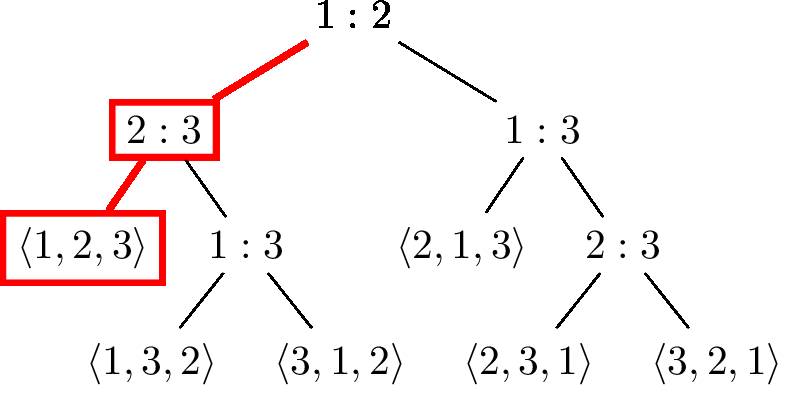
\includegraphics[scale=.35]{res/test.jpg}
	\captionof{figure}{Albero di decisione di un algoritmo che opera su tre elementi.}\label{fig:alberodecisione}
\end{center}

In un albero di decisione, ogni nodo interno è annotato con $i:j$ per qualche $i$ e $j$ nell'intervallo $1 \leq i,j \leq n$, dove $n$ è il numero di elementi nella sequenza di input. Ogni foglia è annotata con una permutazione $\langle \pi(1),\pi(2),...,\pi(n) \rangle$.

L'esecuzione dell'algoritmo di ordinamento corrisponde a tracciare un cammino semplice dalla radice dell'albero di decisione fino a una foglia. Ogni nodo interno rappresenta un confronto $a_{i} \leq a_{j}$. Il sottoalbero sinistro detta i successivi confronti per $a_{i}\leq a_{j}$; il sottoalbero destro detta i successivi confronti per $a_{i}\geq a_{j}$.

Quando raggiunge una foglia, l'algoritmo ha stabilito l'ordinamento $$a_{\pi(1)} \leq a_{\pi(2)} \leq \cdots \leq a_{\pi(n)}$$ Poiché qualsiasi algoritmo di ordinamento corretto deve essere in grado di produrre ogni permutazione del suo input, una \textit{condizione necessaria} affinché un ordinamento per confronti sia corretto è che ciascuna delle $n!$ permutazioni di $n$ elementi appaia come una delle foglie dell'albero di decisione e che ciascuna di queste foglie sia raggiungibile dalla radice attraverso un percorso che corrisponde a una effettiva esecuzione dell'ordinamento per confronti (queste foglie saranno chiamate ``raggiungibili'').

La \textbf{lunghezza del cammino semplice più lungo} dalla radice di un albero di decisione a una delle due foglie raggiungibili rappresenta il \textbf{numero di confronti} che svolge il corrispondente algoritmo di ordinamento nel caso peggiore. Di conseguenza il numero di confronti nel caso peggiore per un dato algoritmo di ordinamento basato sui confronti è \textit{uguale all'altezza del suo albero di decisione.}


\begin{teorbox}
Sia $T$ un albero di decisione che ordina $n$ elementi distinti. $T$ ha un altezza almeno pari a $\Theta(n \log_{2}n)$.
\end{teorbox}


\begin{proof}
	Per quanto detto in precedenza T ha $n!$ foglie, se ne avesse di più sarebbe ridondante, se ne avesse di meno non ha ancora fatto tutti i confronti e quindi sarebbe incompleto. Essendo gli esiti dei confronti solo di due tipi (minore o maggiore) si ha che $T$ è un albero binario (il quale avrà al massimo $2^{h}$ foglie). Da queste informazione possiamo dire dunque che :
	\begin{displaymath}
		n! \leq 2^{h}
	\end{displaymath}
	Per calcolare il tempo medio di un algoritmo basterà quindi dividere la \textbf{lunghezza del percorso esterno} (LPE), ovvero la somma delle lunghezze dei cammini dalla radice alle foglie, per il numero medio di confronti:
	\begin{displaymath}
		T_{M}(n)=\frac{LPE}{n!}
	\end{displaymath}
	Dato un albero saprò calcolare il percorso medio, ma in generale devo trovare un albero che minimizza l'espressione precedente. Poiché non è possibile minimizzare il numero $n$ si può pensare di minimizzare la lunghezza del percorso esterno. Gli alberi completi (vedi \ref{alberi_binari_prop}) rispondono a questa necessità. Infatti questi alberi, fissato un numero di nodi, avranno la minor altezza possibile, minimizzando così la quantità $LPE$.


	In un albero completo valgono le seguenti proprietà:
	\begin{eqnarray}
		N_{h} + N_{h-1} = n!\\
		N_{h} + 2N_{h-1} = 2^{h}
	\end{eqnarray}
	dove $N_{h}$ è il numero di foglie alla profondità $h$ e $N_{h-1}$ è il numero di foglie alla profondità $h$.

	Sottraendo la prima equazione alla seconda si ottiene:
	\begin{equation}
		N_{h-1}= n! - 2^{h}
	\end{equation}
	Abbiamo quindi:
	\begin{eqnarray}
		LPE &=& h \cdot N_{h} + (h-1)N_{h-1} \nonumber \\
		&=& h \cdot N_{h}+ h\cdot N_{h-1} - N_{h-1} \nonumber \\
		&=& h \cdot ( N_{h} + N_{h-1}) - N_{h+1} \nonumber \\
		&=& h \cdot n! - N_{h-1} \nonumber \\
		&=& h \cdot n! - 2^{h} + n!
	\end{eqnarray}

	Il numero medio di confronti sarà allora:
	\begin{eqnarray}
		T_{M}(n)&=&\frac{LPE}{n!} \nonumber \\
		&=& \frac{h \cdot n! - 2^{h} + n!}{n!} \nonumber \\
		&=& h - \frac{2^{h}}{n!}+1 \nonumber
	\end{eqnarray}
	Sapendo che $h= \log n!$ si ha:
	\begin{equation}
		T_{M}(n) = \log n! - \frac{2^{\log n!}}{n!}+1= \log n!
	\end{equation}
	Ma abbiamo già dimostrato che $\log n! = \Theta(n \log n)$ e quindi possiamo concludere dicendo che il tempo di esecuzione di un algoritmo di ordinamento per una sequenza arbitraria di input $n$ non può essere, nel caso medio e nel caso peggiore, migliore di $\Theta(n \log n)$.
\end{proof}


\begin{center}
	\begin{tblr}{hlines,vlines,colspec={lX},row{1}={primary!80!white}}
		\textbf{Algoritmo} & \textbf{Tempo di esecuzione nel caso peggiore} & \textbf{Tempo di esecuzione nel caso medio} \\
		\textbf{\textsc{Insertion Sort}} & $\Theta(n^{2})$ & $\Theta(n^{2})$\\

		\textbf{\textsc{Mergesort}} & $\Theta(n \log n)$& $\Theta(n \log n)$\\

		\textbf{\textsc{Heapsort}} &$O(n \log n)$ & - \\

		\textbf{\textsc{Quicksort}} & $\Theta(n^{2})$ & $\Theta(n \log n)$\\
	\end{tblr}
	\captionof{table}{Confronto dei tempi di esecuzione degli algoritmi di ordinamento}
\end{center}

\chapter{Basi matematiche}
\chapter{Tracce d'esame}\label{chapter_ex}
\subsection{Esame del 17 gennaio 2024}
\begin{enumerate}
\item Si risponda alle seguenti tre domande a risposta multipla, \textbf{motivando brevemente} l'esclusione delle opzioni considerate errate. \textbf{In assenza di una motivazione, le risposte saranno considerate errate.}
\begin{enumerate}
	\item Per ognuno dei seguenti alberi di ricerca, si identifichino le classi di appartenenza tra \textbf{PB} (Perfettamente Bilanciato), \textbf{C} (Completo), \textbf{AVL} e \textbf{RB} (Red Black senza foglie \textsc{NIL}).

	\begin{minipage}{.2\textwidth}
		\centering
		$\tau_{1}$

		\begin{tikzpicture}
			[level distance=6mm,level/.style={sibling distance=20mm/#1}]
			\node{6}
			child{
				node{2}
				child{
					node{1}
					child{
						node{0}
					}
					child[missing]
				}
				child{
					node{4}
					child{
						node{3}
					}
					child{
						node{5}
					}
				}
			}
			child{
				node{7}
			};
		\end{tikzpicture}
	\end{minipage}
	\hfil
		\begin{minipage}{.2\textwidth}
		\centering
		$\tau_{2}$

		\begin{tikzpicture}
			[level distance=6mm,level/.style={sibling distance=20mm/#1}]
			\node{4}
			child{
				node{2}
				child{
					node{1}
					child{
						node{0}
					}
					child[missing]
				}
				child{
					node{3}
				}
			}
			child{
				node{6}
				child{
					node{5}
				}
				child{
					node{8}
					child{
						node{7}
					}
					child[missing]
				}
			};
		\end{tikzpicture}
	\end{minipage}
	\hfil
		\begin{minipage}{.2\textwidth}
			\centering
			$\tau_{3}$

			\begin{tikzpicture}
				[level distance=6mm,level/.style={sibling distance=20mm/#1}]
				\node{4}
				child{
					node{2}
					child{
						node{1}
						child{
							node{0}
						}
						child[missing]
					}
					child{
						node{3}
					}
				}
				child{
					node{5}
					child{
						node{6}
					}
					child[missing]
				};
			\end{tikzpicture}
	\end{minipage}
	\hfil
		\begin{minipage}{.2\textwidth}
			\centering
			$\tau_{4}$

		\begin{tikzpicture}
			[level distance=6mm,level/.style={sibling distance=20mm/#1}]
			\node{5}
			child{
				node{3}
				child{
					node{1}
					child{
						node{0}
					}
					child{
						node{2}
					}
				}
				child{
					node{4}
				}
			}
			child{
				node{7}
				child{
					node{6}
				}
				child[missing]
			};
		\end{tikzpicture}
	\end{minipage}
	\item Si consideri il grafo orientato rappresentato dalle seguenti liste di adiacenza, in cui le liste dei nodi assenti sono vuote (tali vertici non hanno archi uscenti). Si indichi quali delle cinque sequenze di vertici sotto riportate sono ordinamenti topologici e quali no.
	\begin{displaymath}
		\begin{array}{lll}
			a \rightarrow [b] & & a,b,g,i,c,e,d,f,h \\
			b \rightarrow [g,i] & & c,e,a,d,h,b,f,g,i \\
			c \rightarrow [d,e] & & a,b,g,c,e,d,i,h,f \\
			d \rightarrow [g,h] & & a,c,b,e,i,h,f,d,g \\
			e \rightarrow [d,f,h] & & c,a,e,b,d,i,h,g,f
		\end{array}
	\end{displaymath}
	\item Dato l'array di numeri naturali $\mathbf{A} = [\stackrel{0}{7},\stackrel{1}{6},\stackrel{2}{8},\stackrel{3}{5},\stackrel{4}{1},\stackrel{5}{9},\stackrel{6}{8},\stackrel{7}{0},\stackrel{8}{2},\stackrel{9}{4},\stackrel{10}{3},\stackrel{11}{1}]$, si identifichi tra le seguenti configurazioni del vettore $\mathbf{A}$ e degli indici $i$ e $j$ il risultato dell'applicazione della funzione \textsc{Partiziona}$(A,3,8)$ usata nell'algoritmo di \textsc{Quicksort} presentato nel corso.
	\begin{itemize}
		\item $
		\begin{array}{cccccccccccc}
			[\stackrel{0}{7}, &
			\stackrel{1}{6}, &
			\stackrel{2}{8}, &
			\stackrel{3}{2}, &
			\stackrel{4}{1}, &
			\stackrel{5}{0}, &
			\stackrel{6}{8}, &
			\stackrel{7}{9}, &
			\stackrel{8}{5}, &
			\stackrel{9}{4}, &
			\stackrel{10}{3}, &
			\stackrel{11}{1}] \\
			 & %1
			 & %2
			 & %3
			 & %4
			 & %5
			 & %6
			 i j& %7
			 & %8
			 & %9
			 & %10
			 & %11
		\end{array}$
		\item $\begin{array}{cccccccccccc}
			[\stackrel{0}{7},&
			\stackrel{1}{6}, &
			\stackrel{2}{8}, &
			\stackrel{3}{2}, &
			\stackrel{4}{1}, &
			\stackrel{5}{0}, &
			\stackrel{6}{8}, &
			\stackrel{7}{9}, &
			\stackrel{8}{5}, &
			\stackrel{9}{4}, &
			\stackrel{10}{3}, &
			\stackrel{11}{1}] \\
			   %0
			 & %1
			 & %2
			 & %3
			 & %4
			 & %5
			 j& %6
			 i& %7
			 & %8
			 & %9
			 & %10
			 & %11
		\end{array}$
		\item $\begin{array}{cccccccccccc}
			[\stackrel{0}{7}, &
			\stackrel{1}{6}, &
			\stackrel{2}{8}, &
			\stackrel{3}{5}, &
			\stackrel{4}{1}, &
			\stackrel{5}{2}, &
			\stackrel{6}{0}, &
			\stackrel{7}{8}, &
			\stackrel{8}{9}, &
			\stackrel{9}{4}, &
			\stackrel{10}{3}, &
			\stackrel{11}{1}] \\
			  %0
			  & %1
			  & %2
			  & %3
			  & %4
			  & %5
			  & %6
			  j& %7
			  i& %8
			  & %9
			  & %10
			  & %11
		 \end{array}$
		\item $\begin{array}{cccccccccccc}
			[\stackrel{0}{7}, &
			\stackrel{1}{3}, &
			\stackrel{2}{4}, &
			\stackrel{3}{2}, &
			\stackrel{4}{1}, &
			\stackrel{5}{0}, &
			\stackrel{6}{8}, &
			\stackrel{7}{9}, &
			\stackrel{8}{5}, &
			\stackrel{9}{8}, &
			\stackrel{10}{6}, &
			\stackrel{11}{1}] \\
			  %0
			  & %1
			  & %2
			  & %3
			  & %4
			  & %5
			  j& %6
			  i& %7
			  & %8
			  & %9
			  & %10
			  & %11
		 \end{array}$
	\end{itemize}
\end{enumerate}
\item Si risolva la seguente equazione di ricorrenza, calcolandone l'\textbf{andamento asintotico}:
\begin{displaymath}
	T(n) = \begin{cases}
		1 & \text{se $n \leq 1$} \\
		4 \cdot T(\frac{n}{2})+n & \text{altrimenti}
	\end{cases}
\end{displaymath}
\item Si riporti lo pseudo-codice dell'algoritmo di \textbf{visita in profondità su grafo} (con annesso calcolo dei tempi di inizio e fine visita). Inoltre si applichi l'algoritmo al grafo dell'esercizio 1b e si rappresenti graficamente la foresta di visita, dove a ogni nodo è associata la coppia $(d,f)$ dei tempi di inizio ($d$) e fine ($f$) visita.
\item Si scriva un \textbf{algoritmo ricorsivo} che, dati in ingresso un albero binario $T$ contenente numeri interi e due numeri naturali $l_{1} \leq l_{2}$, restituisca la \textbf{somma dei valori} $d$ di tutti quei nodi con $d$ pari e la cui profondità $p$ non sia compresa tra $l_{1}$ ed $l_{2}$. Tale algoritmo dovrà essere efficiente e non far uso né di variabili globali, né di parametri passati per riferimento. Si scriva infine un algoritmo iterativo che simuli precisamente l'algoritmo ricorsivo di cui sopra.
\end{enumerate}


\printindex
\end{document}
